\documentclass{bookest}

\usepackage{hyperref}
\usepackage{amsmath}
\usepackage{amssymb}
\usepackage{amsthm}
\usepackage{graphics}
\usepackage{graphicx}
\usepackage{floatrow}
\usepackage{tikz}
\usepackage{color}
\usepackage{algorithm}
\usepackage{algorithmicx}
\usepackage{algpseudocode}
\usepackage{caption}
\usepackage{subcaption}
\usepackage{exercise}
\usepackage{chngcntr}
\usepackage{array, booktabs}
\usepackage{varwidth}
\usepackage{multicol}
\usepackage{float}
\usepackage{eurosym}



\newcommand{\reals}{\mathbb{R}}
\newcommand{\integers}{\mathbb{Z}}
\newcommand{\symm}{\mathbb{S}}  % symmetric matrices

\newcommand{\rank}{\mathop{\bf rank}}
\newcommand{\tr}{\mathop{\bf tr}}
\newcommand{\diag}{\mathop{\bf diag}}
\renewcommand{\rank}{\mathop{\bf rank}}
\newcommand{\conv}{\mathop{\bf conv}}
\newcommand{\spans}{\mathop{\bf span}}
\newcommand{\nulls}{\mathop{\bf null}}
\newcommand{\clo}{\mathop{\bf clo}}

\renewcommand{\det}{\mathop{\bf det}}
\newcommand{\proj}{\mathop{\bf proj}}
\newcommand{\argmin}{\mathop{\rm argmin}}
\newcommand{\argmax}{\mathop{\rm argmax}}
\newcommand{\epi}{\mathop{\bf epi}} % epigraph
\newcommand{\dom}{\mathop{\bf dom}} % domain
\newcommand{\intr}{\mathop{\bf int}}
\newcommand{\bou}{\mathop{\bf bou}}

\newcommand{\mini}{\mathop{\text{min.~}}}
\newcommand{\maxi}{\mathop{\text{max.~}}}
\newcommand{\minf}{\mathop{\text{minimize~}}}
\newcommand{\maxf}{\mathop{\text{maximize~}}}
\newcommand{\st}{\mathop{\text{s.t.:~}}}
\newcommand{\stf}{\mathop{\text{subject to:~}}}

\newcommand{\braces}[1]{\left\{ #1 \right \}}
\newcommand{\brackets}[1]{\left[ #1 \right]}
\newcommand{\floor}[1]{\lfloor #1 \rfloor}
\newcommand{\ceil}[1]{\lceil #1 \rceil}

\newcommand{\lb}{\linebreak}

\newtheorem{theorem}{Theorem}
\newtheorem*{theorem*}{Theorem}
\newtheorem{proposition}[theorem]{Proposition}
\newtheorem*{remark}{Remark}
\newtheorem{assumption}[theorem]{Assumption}
\newtheorem{definition}[theorem]{Definition}
\newtheorem{lemma}[theorem]{Lemma}
\newtheorem{corollary}[theorem]{Corollary}




\parindent 0cm
\parskip 0.15cm
\topmargin 0.2cm
\oddsidemargin 1cm
\evensidemargin 0.5cm
\textwidth 15cm
\textheight 21cm
\definecolor{blue}{rgb}{0.23,0.58,0.89}


\begin{document}

	%% temporary titles
% command to provide stretchy vertical space in proportion
\newcommand\nbvspace[1][3]{\vspace*{\stretch{#1}}}

% allow some slack to avoid under/overfull boxes
\newcommand\nbstretchyspace{\spaceskip0.5em plus 0.25em minus 0.25em}

% To improve spacing on title pages
\newcommand{\nbtitlestretch}{\spaceskip0.6em}

\thispagestyle{empty}

\begin{center}
	\bfseries
	\nbvspace[1]
	\Huge
	{\nbtitlestretch\huge
	OPTIMISATION NOTES}
	
	\nbvspace[1]
	\normalsize
	
	A COMPILATION OF LECTURE NOTES \\
	FROM GRADUATE-LEVEL \\
	OPTIMISATION COURSES 
	
	\nbvspace[1]
	\small TAUGH BY\\
	\Large FABRICIO OLIVEIRA\\[0.5em]
	\footnotesize ASSOCIATE PROFESSOR OF OPERATIONS RESEARCH\\
	AALTO UNIVERSITY, SCHOOL OF SCIENCE
	
	\nbvspace[2]
	
%	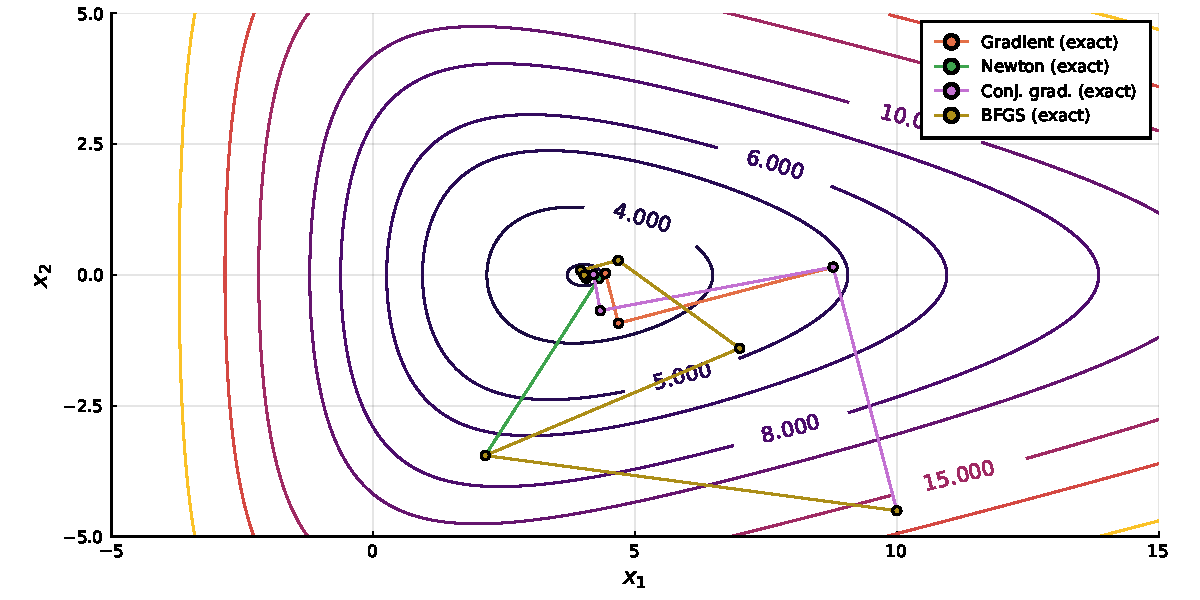
\includegraphics[width=1.5in]{part_2/chapter_5/figures/all_methods_exact}
	
%	\nbvspace[3]
	
	\normalsize
	
	SOURCE CODE AVAILABLE AT\\
	
	\large
	{\color{blue}\href{https://github.com/gamma-opt/optimisation-notes}{github.com/gamma-opt/optimisation-notes}}
	
	\nbvspace[1]
\end{center}





	\tableofcontents
	
	\part{Linear optimisation}
	
	\chapter{Introduction} \label{chapter_1}
	\section{What is optimisation?}

An optimisation is one of these words that has many meanings, depending on the context you take as a reference. In the context of this course, optimisation refers to \emph{mathematical optimisation}, which is a discipline of applied mathematics.

In mathematical optimisation, we build upon concepts and techniques from calculus, analysis, linear algebra, and other domains of mathematics to develop methods that allow us finding values for variables within a given domain that maximise (or minimise) the value of a function. In specific, we are trying to solve the following general problem:
%
\begin{align}
    \mini & f(x) \label{eq:opt_prob} \\
    \text{s.t.}   &x \in X. \nonumber
\end{align}
%
%where $x \in \reals^n$ is a vector of $n$ \emph{variables}, $f:\mathbb{R}^n \mapsto \reals$ is a \emph{function} to be optimised (minimised) and $X \subseteq \reals^n$ is a \emph{domain} containing acceptable values for $x$.

In a general sense, these problems can be solved by employing the following strategy:
%
\begin{enumerate}
    \item Analysing properties of functions under specific domains and deriving the conditions that must be satisfied such that a point $x$ is a candidate optimal point.
    \item Applying numerical methods that iteratively searches for points satisfying these conditions. 
\end{enumerate}
%
This idea is central in several domains of knowledge, and very often are defined under area-specific nomenclature. Fields such as economics, engineering, statistics, machine learning and, perhaps more broadly, operations research, are intensive users and developers of optimisation theory and applications. 

\subsection{Mathematical programming and optimisation}

Operations research and mathematical optimisation are somewhat intertwined, as they both were born around a similar circumstance. %(Include something on the history of OR)

I like to separate \emph{mathematical programming} from (mathematical) \emph{optimisation}. Mathematical programming is a modelling paradigm, in which we rely on (very powerful, I might add) analogies to model \emph{real-world} problems. In that, we look at a given decision problem considering that
%
\begin{itemize}
    \item \emph{variables} represent \emph{decisions}, as in a business decision or a course of action. Examples include setting the parameter of (e.g., prediction) model, production systems layouts, geometries of structures, topologies of networks, and so forth; 
    \item \emph{domain} represents business rules or \emph{constraints}, representing logic relations, design or engineering limitations, requirements, and such; 
    \item function is an \emph{objective function} that provides a measure of solution quality.  
\end{itemize}
%    
With these in mind, we can represent the decision problem as a \emph{mathematical programming model} of the form of \eqref{eq:opt_prob} that can be solved using \emph{optimisation} methods. From now on, we will refer to this specific class of models as mathematical optimisation models, or optimisation models for short. We will also use the term to \emph{solve the problem} to refer to the task of finding optimal solutions to optimisation models.

This course is mostly focused on the optimisation techniques employed to find optimal solutions for these models. As we will see, depending on the nature of the functions $f$ and $g$ that are used to formulate the model, some methods might be more or less appropriate. Further complicating the issue, for models of a given nature, there might be alternative algorithms that can be employed and with no generalised consense whether one method is generally better performing than another.

\subsection{Types of mathematical optimisation models}

In general, the simpler the assumptions on the parts forming the optimisation model, the more efficient are the methods to solve such problems. 

Let us define some additional notation that we will use from now on. Consider a model in the general form
%
\begin{align*}
	\mini & f(x) \\
	\st   & g_i(x) \leq 0, i = 1, \dots, m \\
	      & h_i(x) = 0, i = 1, \dots, l \\
	      & x \in X,  
\end{align*}
%
where $f: \reals^n \mapsto \reals$ is the objective function, $g:\reals^m \mapsto \reals^m$ is a collection of $m$ inequality constraints and $h: \reals^n \mapsto \reals^l$ is a collection of $l$ equality constraints.

{\bf Remark:} in fact, every inequality constraint can be represented by an equality constraint by making $h_i(x) = g_i(x) + x_{n+1}$ and augmenting the decision variable vector $x \in \reals^n$ to include the slack variable $x_{n+1}$. However, since these constraints are of very different nature, we will explicitly represent both whenever necessary.

The most general types of models are the following. We also use this as an opportunity to define some (admittedly confusing) nomenclature from the field of operations research that we will be using in these notes.
%
\begin{enumerate}
    \item \emph{Unconstrained models:} in these, the set $X = \reals^n$ and $m=l=0$. These are prominent in, e.g., machine learning and statistics applications, where $f$ represents a measure of model fitness or prediction error.  
    \item \emph{Linear programming (LP):} presumes linear objective function. $f(x) = c^\top x$ and constraints $g$ and $h$ affine, i.e., of the form $a_i^\top x - b_i$, with $a_i \in \reals^n$ and $b \in \reals$. Normally, $X = \braces{x \in \reals^n \mid x_j \geq 0, j = 1,\dots, n}$ enforce that decision variables are constrained to be the nonnegative orthant.
    \item \emph{Nonlinear programming (NLP):} some or all of the functions $f$, $g$, and $h$ are nonlinear.
    \item \emph{Mixed-integer (linear) programming (MIP):} consists of an LP in which some (or all) of the variables are constrained to be integers. In other words, $X \subseteq \reals^k \times \integers^{n-k}$. Very frequently, the integer variables are binary terms, i.e., $x_i \in \braces {0,1}$, for $i = 1,\dots, n-k$ and are meant to represent true-or-false or yes-or-no conditions.
    \item \emph{Mixed-integer nonlinear programming (MINLP):} are the intersection of MIPs and NLPs.  
\end{enumerate}

{\bf Remark:} notice that we use the vector notation $c^\top x = \sum_{j \in J} c_j x_j$, with $J = \braces{1,\dots,N}$. This is just a convenience for keeping the notation compact. 


\section{Linear programming applications}

We will consider now a few examples of liner programming models with somewhat general structure. Many of these examples have features that can be combined into more general models.


\subsection{Resource allocation}

Most linear programming (LP) problems, can be interpreted as a \emph{resource allocation} problem. In that, we are interested in defining an optimal allocation of resources (i.e., a plan) that maximises return or minimise costs and satisfy allocation rules. 

Specifically, let $I = \braces{1, \dots, i, \dots, M}$ by a set of resources that can be combined to produce products in the set $J = \braces{1, \dots, j, \dots, N}$. Assume that we are given a return per unit of product $c_j$, $\forall j\in J$ and a list of $a_{ij}$, $\forall i \in I, \forall j \in J$ describing which and how much of the resources $i \in I$ are required for making product $j \in J$. Assume that the availability of resource $b_i$, $\forall i\in I$, is known. 

Our objective is to define the amounts $x_j$ representing the production of $j \in J$. We would like to define those in a way that we optimise the resource allocation plan quality (in our case, maximise return from the production quantities $x_j$) while making sure the amount produced do not exceed the availability of resources. For that, we need to define: 

The \emph{objective function}, which measures the \emph{quality} of a production plan. In this case, the total return for a given plan is given by:
%
\begin{equation*}
	\maxi \sum_{j \in J}c_jx_j \Rightarrow c^\top x,
\end{equation*}
%
where $c = [c_1, \dots, c_{N}]^\top$ and $x = [x_1, \dots, x_{N}]^\top$ are $n$-sized vectors.


Next, we need to define \emph{constraints} that state the conditions for a plan to be \emph{valid}. In this context, a valid plan is a plan that does not utilise more than the amount of resources $b_i$, $\forall i \in I$ available. This can be expressed as the collection (one for each $i \in I$) of linear inequalities
%
\begin{equation*}
	\st \sum_{j \in J} a_{ij}x_j \leq b_i, \forall i \in I	\Rightarrow	Ax \leq b,
\end{equation*}
%
where $a_{ij}$ are the components of the $M \times N$ matrix $A$ and $b = [b_1,\dots, b_M]^\top$. Furthermore, we also must require that $x_i \geq 0, \forall i \in I$.                                                                                                         

Combining the above, we obtain the generic formulation that will be used throughout this text to represent linear programming models:
%
\begin{align}
	\maxi & c^\top x  \label{p1c1:eq:LP_objective} \\
	\st   & Ax \leq b \label{p1c1:eq:LP_constraint} \\
		  & x \geq 0. \label{p1c1:eq:LP_domain}
\end{align}
%

\subsubsection{Illustrative example: the paint factory problem}
 
Let us work on a more specific example, that will be useful for illustrating some important concepts related to the geometry of linear programming problems.

A paint factory produces \emph{exterior} and \emph{interior paint} from raw materials \emph{M1} and \emph{M2}. The \emph{maximum demand} for interior paint is 2 tons/day. Moreover, the amount of interior paint produced \emph{cannot exceed} that of exterior paint by more than 1 ton/day. 

Our goal is to determine optimal paint production plan. Table \ref{p1c1:tab:paint_factory_problem_data} summarises the data to be considered. Notice the constraint that must be imposed to represent the daily availability of paint.

\begin{table}[h]
	\begin{tabular}{rccc} \hline
	&\multicolumn{2}{c}{material (ton)/paint (ton)}\\ \hline
	& exterior paint & interior paint & daily availability (ton)\\ \hline
	material M1 & 6 & 4 & 24\\
	material M2 & 1 & 2 & 6\\ \hline
	profit (\$1000 /ton) & 5 & 4\\ \hline
	\end{tabular}
	\caption{Paint factory problem data} \label{p1c1:tab:paint_factory_problem_data}
\end{table}

Notice that the paint factory problem is an example of a resource allocation problem. Perhaps one aspect that is somewhat dissimilar is the constraint representing the production rules regarding the relative amounts of interior and exterior paint. Notice however, that this type of constraint also has the same format as the more straightforward resource allocation constraints.  

Let $x_1$ be amount produced of exterior paints (in tons) and $x_2$ the amount of interior paints. The complete model that optimises the daily production plan of the paint factory is:
%
\begin{flalign}
	\maxi z = \ & 5x_1 + 4x_2 \label{p1c1:eq:constM1}\\
	\st & 6x_1 + 4x_2 \leq 24 \label{p1c1:eq:constM2}\\
	& x_1 + 2x_2 \leq 6 \\
	& x_2 - x_1 \leq  1 \\
	& x_2 \leq 2 \\
	& x_1, x_2 \geq 0
\end{flalign}
%
Notice that paint factory model can also be \emph{compactly represented} as in \eqref{p1c1:eq:LP_objective}--\eqref{p1c1:eq:LP_domain}, where
%
\begin{equation*}
	c = [5, 4]^\top, \ x = [x_1, x_2]^\top, \ A = \begin{bmatrix} 6 & 4 \\ 1 & 2 \\ -1 & 1 \\0 & 1 \end{bmatrix}, \text{ and } b = [24, 6, 1, 2]^\top.	
\end{equation*}
%


\subsection{Transportation problem}

Another important class of linear programming problems are those known as transportation problems. These problems are often model using the abstraction of graphs, since they consider a network of nodes and arcs through which some flow must be optimised. Transportation problems have several important characteristics that can be exploit to design specialised algorithms, the so-called \emph{transportation simplex} method. Although we will not discuss these methods in this text, the simplex method (and its variant dual simplex) will be in the centre of our developments later on. Also, modern solvers have more and more relegate transport simplex methods in their development, as dual simplex has consistently shown to perform similarly in the context of transportation problems, despite being a far more general method. 

The problem can be summarised as follows. We would like to plan production and distribution of a certain product, taking into account that the transportation cost is known (e.g., proportional to distance travelled), the factories (or source nodes) have a capacity limit and the clients (or demand nodes) have known demands. Figure \ref{p1c1:fig1:transport_network} illustrate a small network with two factories, located in San Diego and Seattle, and three demand points, located in New York, Chicago, and Miami. Table \ref{p1c1:tab:transport_problem_data} presents the data related to the problem. 
%
\begin{figure}[h]
	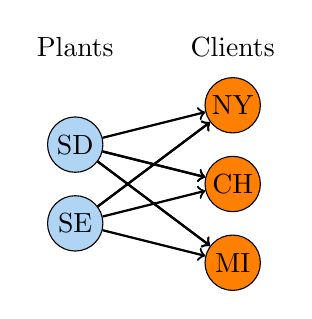
\begin{tikzpicture}[scale=1,
		node/.style={circle, fill=blue!40, draw, minimum size=2em, inner sep=1pt},
		node2/.style={circle, fill=orange, draw, minimum size=2em, inner sep=1pt}] 
    	\node[above] at (0, 3.5) {Plants};                                                                                  
    	\node[above] at (2, 3.5) {Clients};
	    \node[node] (1) at (0, 1.5) {SE};
	    \node[node] (2) at (0, 2.5) {SD};
	    \node[node2] (3) at (2, 3) {NY};
	    \node[node2] (4) at (2, 2) {CH};
	    \node[node2] (5) at (2, 1) {MI};
	    \foreach \x in {1,...,2} {
	       \foreach \y in {3,...,5} {
	          \draw[->, thick] (\x) -- (\y);
	          }}      
	    \draw[->, thick] (1) -- (3);
	    \draw[->, thick] (2) -- (4);
	    \draw[->, thick] (2) -- (5);                            
	\end{tikzpicture}
	\caption{Schematic illustration of a network with two source nodes and three demand nodes} \label{p1c1:fig1:transport_network}    
\end{figure}
%
\begin{table}
	\begin{tabular}{r|ccc|c}
    	& & {\it Clients} &\\\hline
    	{\it Factory} & NY & Chicago & Miami & Capacity \\\hline
    	Seattle & 2.5      & 1.7    & 1.8   & 350 \\
    	San Diego & 3.5 & 1.8 & 1.4 & 600 \\\hline
    	Demands & 325 & 300 & 275 & - \\\hline
	\end{tabular}
	\caption{Problem data: unit transportation costs, demands and capacities} \label{p1c1:tab:transport_problem_data}
\end{table}

To formulate a linear programming model representing the transportation problem, let $i \in I = \{\text{Seattle}, \text{San Diego}\}$ be the index set representing factories. Similarly, let $j \in J = \{\text{New York}, \text{Chicago}, \text{Miami}\}$.

The decisions in this case are represented by $x_{ij}$ be the amount produced in factory $i$ and sent to client $j$. Such a distribution plan can then be assessed by its total transportation cost, which is given by
%
$$ 
\mini z = 2.5x_{11} + 1.7x_{12} + 1.8x_{13} + 3.5x_{21} + 1.9x_{22} + 1.4x_{23}.
$$
%
The total transportation cost can be more generally represented as
%
$$
\mini z = \sum_{i \in I}\sum_{j \in J}c_{ij}x_{ij}
$$
%
where $c_{ij}$ is the unit transportation cost from $i$ to $j$.
%
The problem has two types of constraints that must be observed, relating to the supply capacity and demand requirements. These can be stated as the following linear constraints
%
\begin{align*}
	& x_{11} + x_{12} + x_{13} \leq 350 \text{ (capacity limit in Seattle)}\\
	& x_{21} + x_{22} + x_{23} \leq 600 \text{ (capacity limit in San Diego)}\\
	& x_{11} + x_{21} \geq 325 \text{ (demand in New York)}\\
	& x_{12} + x_{22} \geq 300 \text{ (demand in Chicago)}\\
	& x_{13} + x_{23} \geq 275 \text{ (demand in Miami)}.
\end{align*}
%
These constraints can be expressed in the more compact form
%
\begin{align}
	& \sum_{j \in J} x_{ij} \leq C_i, \forall i  \label{p1c1:eq:transportation_constraint_supply}\\
	& \sum_{i \in I} x_{ij} \geq D_j, \forall j, \label{p1c1:eq:transportation_constraint_demand}
\end{align}

where $C_i$ is the production capacity of factory $i$ and $D_j$ is the demand of client $j$. Notice that the terms on the lefthand side in \eqref{p1c1:eq:transportation_constraint_supply} accounts for the total production in each of the source nodes $i \in I$. Analogously, in constraint \eqref{p1c1:eq:transportation_constraint_demand}, the term on the left accounts for the total of the demand satisfied at the demand nodes $j \in J$. Using an optimality argument stating that any solution for which, for any $j \in J$, $\sum_{i \in I} x_{ij} > D_j$ can be improved by making $\sum_{i \in I} x_{ij} = D_j$. This show that his constraint under these conditions will always be satisfied as an equality constraint instead, and could be replaced like such. 

The complete transportation model for the example above can be stated as 
%
\begin{align*}
	\mini z = \ &2.5x_{11} + 1.7x_{12} + 1.8x_{13} + 3.5x_{21} + 1.9x_{22} + 1.4x_{23} \\
	\st & x_{11} + x_{12} + x_{13} \leq 350, \ 
	x_{21} + x_{22} + x_{23} \leq 600\\
	& x_{11} + x_{21} \geq 325, \ x_{12} + x_{22} \geq 300, \ x_{13} + x_{23} \geq 275\\
	& x_{11}, \dots, x_{23} \geq 0.
\end{align*}
%

Or, more compactly, in the so called \emph{algebraic (or symbolic) form}
%
\begin{align*}
	\mini z = \ &\sum_{i \in I}\sum_{j \in J}c_{ij}x_{ij}\\
	\st & \sum_{j \in J} x_{ij} \leq C_i, \forall i\\
	& \sum_{i \in I} x_{ij} \geq D_j, \forall j\\
	&x_{ij} \geq 0, \forall i \in I, \forall j \in J.
\end{align*}
%
One interesting aspect to notice regarding algebraic forms is that they allow to represent the main structure of the model while being independent of the instance being considered. For example, regardless of whether the instance would have 5 or 50 nodes, the algebraic formulation is the same, allowing for detaching the problem instance (in our case the 5 node network) from the model itself. Moreover, most computational tools for mathematical programming modelling (hereinafter referred to simply as modelling - like JuMP) requires the user to define the optimisation model using this algebraic representation.

Algebraic forms are the main form in which we will specify optimisation models. This abstraction is a peculiar aspect of mathematical programming, and is perhaps one the main features the fact that one must \emph{formulate} models for each specific setting, which can be done in multiple ways and might have consequences for how well computationally an algorithm performs. Further in this text we will discuss this point in more detail.  


\subsection{Production planning (lot-sizing)}


Production planning problems, commonly referred to as lot-sizing problems in contexts related to industrial engineering, consider problems where a planning horizon is taken into consideration. Differently from the previous examples, lot-sizing problems allow for the consideration of a time flow aspect, in which production that is made in the past can be ``shifted'' to a future point in time by means of inventories (i.e., stocks). Inventories are important because they allow for taking advantage of different prices at different time periods, considering production capacity limitations, or to prepare against uncertainties in the future (e.g., uncertain demands).

The planning horizon is represented buy a collection of chronologically ordered elements $t \in \braces{1,\dots, T}$ representing a set of uniformly-sized time periods (e.g., months or days). Then let us define the decision variables $p_t$ as the amount produced in period $t$ and $s_t$ the amount stored in period $t$, which is available for use in periods $t' > t$. These decisions are governed by two costs: $P_t$, $\forall t \in T$ representing the production cost in each time period $t$ and the unit holding cost $H$, that is, how much it costs to hold one unit of product for one time period. 

Our objective is to satisfy the demands $D_t$, $\forall t \in T$ at the minimum possible cost. Figure \ref{p1c1:fig:lot-sizing_diagram}	provides a schematic representation of the process to be modelled. Notice that each node represents a material balance to be considered, that is, that at any period $t$, the total produced plus the amount held in inventory from the previous period ($t-1$) must  be the same as the amount used to satisfy the demand plus the amount held in inventory for the next period ($t+1$). 	
   
\begin{figure}[h]
	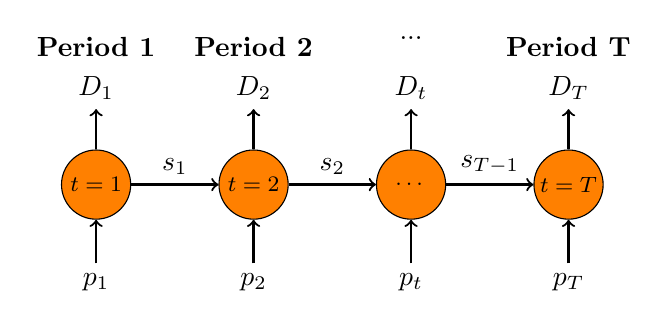
\begin{tikzpicture}[scale=1,
	node/.style={circle, fill=orange, draw, minimum size=2.5em, inner sep=1pt, font = \footnotesize}] 
		\node[below] at (0, 3) {\bf Period 1};                                                                                  
		\node[below] at (2, 3) {\bf Period 2};
		\node[below] at (4, 3) {...};
    	\node[below] at (6, 3) {\bf Period T};
    	\node[below] (11) at (0, 0) {$p_1$};                                                                                  
		\node[below] (21) at (2, 0) {$p_2$};
		\node[below] (31) at (4, 0) {$p_t$};
    	\node[below] (41) at (6, 0) {$p_T$};
    	\node[below] (12) at (0, 2.5) {$D_1$};                                                                                  
		\node[below] (22) at (2, 2.5) {$D_2$};
		\node[below] (32) at (4, 2.5) {$D_t$};
	    \node[below] (42) at (6, 2.5) {$D_T$};	    
		\node[node] (1) at (0, 1) {$t=1$};
		\node[node] (2) at (2, 1) {$t=2$};
		\node[node] (3) at (4, 1) {$\dots$};
		\node[node] (4) at (6, 1) {$t=T$};
		\draw[->, thick] (1) -- node[above] {$s_1$} (2);
		\draw[->, thick] (2) -- node[above] {$s_2$} (3) ;
		\draw[->, thick] (3) -- node[above] {$s_{T-1}$}(4);
		\draw[->, thick] (11) -- (1);
		\draw[->, thick] (21) -- (2);
		\draw[->, thick] (31) -- (3);
		\draw[->, thick] (41) -- (4);   
		\draw[->, thick] (1) -- (12);
		\draw[->, thick] (2) -- (22);
		\draw[->, thick] (3) -- (32);
		\draw[->, thick] (4) -- (42);                                     
	\end{tikzpicture}                    
	\caption{A schematic representation of the lot-sizing problem. Each node represents the material balance at each time period $t$.} \label{p1c1:fig:lot-sizing_diagram}		
\end{figure}

The production planning problem can be formulated as
%
\begin{flalign*}
	\mini & \sum_{t \in T} \left[C_t p_t + H s_t\right] \\
	\st 	  & p_t + s_{t-1} = D_t + s_t, \ \forall t \in T \\
	      & p_t, h_t \geq 0, \ \forall t \in T .	
\end{flalign*}
%

A few points must be considered carefully when dealing with lot-sizing problems. First, one must carefully consider boundary condition, that is what the model is deciding in time periods $t = T$ and what is the initial initial inventory (carried from $t=0$). While the former will be seen by the model as the ``end of the world'' and thus will realise that optimal inventory levels must be zero, the latter might considerable influence how much production is needed during the planning horizon $T$. These must be observed and handled accordingly. 
 


\section{The geometry of LPs - graphical method} 

Let us now focus our attention to the geometry of linear programming (LP) models. As it will become evident later one, LP models have a very peculiar geometry that is exploited by one of the most widespread methods to solve them. 

\subsection{The graphical method}

In order to create a geometric intuition, we will utilise a graphical representation of the resource allocation example (the paint factory problem). But first, recall the general LP formulation \eqref{p1c1:eq:LP_objective}--\eqref{p1c1:eq:LP_domain}, where $A$ is an $m \times n$ matrix, and $b$, $c$, and $x$ have suitable dimensions. Let $a_i$ be one of the $m$ rows of $A$. Notice each constraint $a_i^\top x \leq b_i$ defines a closed half-space, with boundary defined by a hyperplane $a_i^\top x= b_i$, $\forall i \in I = \braces{1,\dots,m} \equiv [m]$. By plotting all of these closed half-spaces we can see that their intersection will form the \emph{feasible region} of the problem, that is, the (polyhedral) set of point that satisfy all constraints $Ax \le b$. 


Figure \ref{p1c1:fig:feasible_region_plot} provides a graphical representation of the feasible region of the paint factory problem. 
%
\begin{figure}[h]
	\begin{subfigure}{0.45\textwidth}
		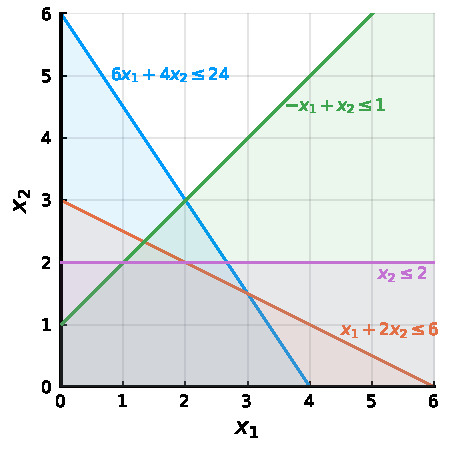
\includegraphics[scale=0.99]{./part_1/chapter_1/figures/ex2_c4.pdf}	
		\caption{}
	\end{subfigure}
	\begin{subfigure}{0.45\textwidth}
		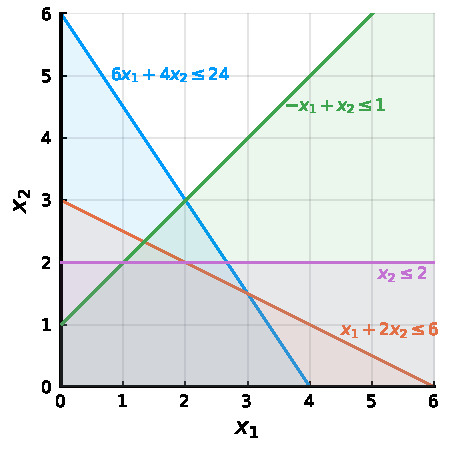
\includegraphics[scale=0.99]{./part_1/chapter_1/figures/ex2_c4.pdf}
		\caption{}		
	\end{subfigure}
	\caption{The feasible region of the paint factory problem, represented as the intersection of the four closed-half spaces formed by each of the constraints. Notice how the feasible region is a polyhedral set in $\reals^2$, as there are two decision variables ($x_1$ and $x_2$).} \label{p1c1:fig:feasible_region_plot}	
\end{figure}
%

We can use this visual representation to find the optimal solution for the problem, that is, the point $(x_1,x_2)$ within the feasible set such that the objective function value is minimal. For that, we must consider how the objective function $z = c^\top x$ can be represented in the $(x_1, x_2)$-plane. Notice that the objective function forms a hyperplane in $(x_1, x_2, z) \subset \reals^3$, of which we can plot level curves (i.e., projections) onto the $(x_1, x_2)$-plane. Figure \ref{p1c1:fig:level_curves_a} shows the plotting of three level curves, for $z= 5, 10$, and $15$. 
%
\begin{figure}
	\begin{subfigure}{0.45\textwidth}
		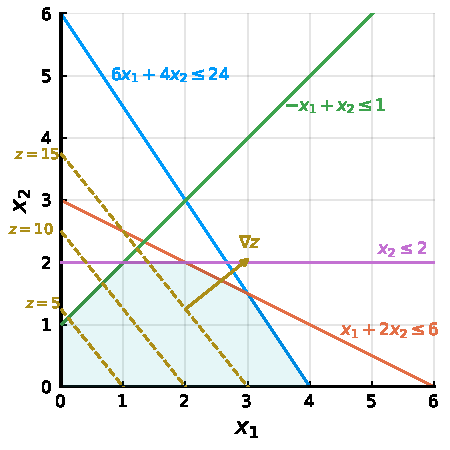
\includegraphics[scale=0.99]{part_1/chapter_1/figures/ex2_c5.pdf}  
		\caption{} \label{p1c1:fig:level_curves_a}	
	\end{subfigure}
	\begin{subfigure}{0.45\textwidth}
		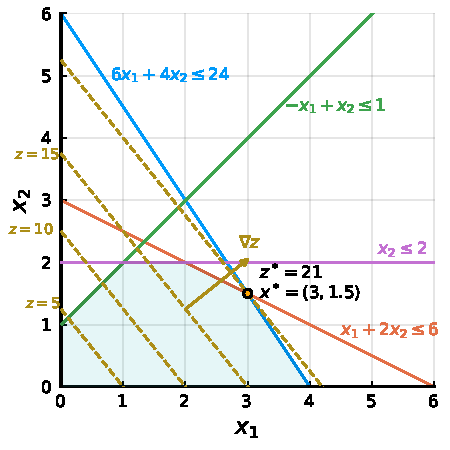
\includegraphics[scale=0.99]{part_1/chapter_1/figures/ex2_complete.pdf}
		\caption{} \label{p1c1:fig:level_curves_b}	 
	\end{subfigure}
	\caption{Graphical representation of some of the level curves of the objective function $z = 5x_1 + 4x_2$. Notice that the constant gradient vector $\nabla z = (5,4)^\top$ points to the direction in which the level curves increase in value. The optimal point is represented by $x^*=(3, 1.5)^\top$ with the furthermost level curve being that associated with the value $z^* = 21$}	
\end{figure}
%
This observation provides us with a simple graphical method to find the optimal solution of linear problems. One must simply sweep the feasible region in the direction of the gradient $\nabla z=[\frac{\partial z}{\partial x_1},\frac{\partial z}{\partial x_2}]^\top=[5,4]^\top$ (or opposite to it, if minimising) until one last point (or edge) or contact remains, meaning that the whole of the feasible region is behind that furthermost level curve. Figure \ref{p1c1:fig:level_curves_b} illustrates the processing of finding the optimal solution for the paint factory problem.

The graphical method is important because it allows to observe several key features that are going to be used later on when we define a method that can search for optimal solutions for LP problems. The first is related to the notion of active or inactive constraints. We say that a constraint is \emph{active} if, at the optimum, the constraint is satisfied as an equality. For example, the constraints $6x_1 + 4x_2 \leq 24$ and $x_1 + 2x_2 \leq 6$ are active at the optimum $x^* = (3, 1.5)$, since $6(3) + 4(1.5) = 24$ and $3 + 2(1.5) = 6$. An active constraint indicates that the resource (or requirement) represented by that constraint is being fully depleted (or minimally satisfied). 

Analogously, \emph{inactive constraint} are constraints that are satisfied as strict inequalities at the optimum. For example, the constraint $-x_1 + x_2 \leq 1$ is inactive at the optimum, as $-(3) + 1.5 < 1$. In this case, an inactive constraint represents a resource (or requirement) that is not fully depleted (or is over satisfied).


\subsection{Geometrical properties of LPs}

One striking feature concerning the geometry of LPs that becomes evident when we analyse the graphical method is that the number of candidate solutions is not infinite, but yet, only \emph{a finite set} of points are potential candidates for optimal solution. This is because the process of sweeping in the direction of the gradient will, in general, lead to a unique solution that must lie on a vertex of the polyhedral feasible set. The only exceptions are either when the gradient $\nabla z$ happens to be perpendicular to a facet of the polyhedral set (and in the direction of the sweeping) or in case the sweeping direction is not bounded by some of the facets of the polyhedral set. These exceptional cases will be discussed in more detail later on, but the observation still holds.

In the graphical example (i.e., in $\reals^2$), notice how making $n = 2$ constraints active out of $m = 4$ constraints \emph{forms a vertex}. However, not all vertices are feasible. This allows us to devise a mechanism to describe vertices (by activating $n$ of the $m$ constraints) which we could exhaustively test and select the best. The issue however, is that the number of candidates increases \emph{exponentially} with the number of constraints and variables	 of the problem, which would quickly become computationally infeasible. As we will see, it turns out that this search idea can be made considerably efficient and the underlying framework of the \emph{simplex method}, however there are worst-case settings where the method does need to consider every single vertex.

The simplex method exploits the above idea to \emph{heuristically} search for solutions by selecting $n$ constraints to be active from the $m$ constraints available. Starting from an initial selection of constraints to be active, it selects one inactive constraint to activate and one to deactivate in a way that improvement in the objective function can observed while feasibility is maintained. This process repeats until no improvement can be observed. When such is the case, the \emph{geometry} of the problem guarantees \emph{(global) optimality}. In the following chapters we will concentrate on defining algebraic objects that we will use to develop the simplex method.



	
	\chapter{Basics of Linear Algebra} \label{chapter_2}
	\section{Basics of linear problems}

As we have seen in the previous chapter, the feasible region of a linear programming problem can be represented as
%
\begin{equation} \label{p1c2:eq:feasible_region_inequality}
	Ax \leq b,	
\end{equation}
%
where $A$ is a $m \times n$ matrix, $x$ is a $n$-dimensional column vector (or more compactly, $x \in \reals^n$), and $b$ is an $m$-dimensional column vector ($b \in \reals^m$). Notice that $\leq$ is considered component-wise.

Before introducing the simplex method, let us first revisit a few key elements and operations that we will use in the process. The first of them is presented in Definition \ref{p1c2:def:matrix_inversion}.
%
\begin{definition}[Matrix inversion] \label{p1c2:def:matrix_inversion}
	Let $A$ be a square $n \times n$ matrix. $A^{-1}$ is the \emph{inverse matrix} of $A$ if it exists and $AA^{-1} = I$, where $I$ is the identity matrix.
\end{definition}
%
Matrix inversion is the ``kingpin'' of linear (and nonlinear) optimisation. As we will see later on, being able to perform efficient matrix inversion operations (in reality, operations that are equivalent to matrix inversion but that can exploit the matrix structure to be made faster) is of utmost importance for developing a linear optimisation solver. 

Another important concept is the notion of \emph{linear independence}. We formally state when a collection of vectors is said to be linearly independent (or dependent) in Definition \ref{p1c2:def:linear_independence}. 

%
\begin{definition}[Linearly Independent vectors] \label{p1c2:def:linear_independence}
	The vectors $\braces{x_i}_{i=1}^k \in \reals^n$  are \emph{linearly dependent} if there exist real numbers $\braces{a_i}_{i=1}^k$ with $a_i \neq 0$ for at least one $i \in \braces{1,\dots, k}$ such that
	$$
		\sum_{i=1}^k a_i x_i= 0;
	$$
	otherwise, $\braces{x_i}_{i=1}^k$ are linearly independent.
\end{definition}

In essence, for a collection of vectors to be linearly independent it must be so that none of the vectors in the collection can be expressed as a combination (that is multiplying the vectors by nonzero scalars and adding them) of the others. This is simpler to see in $\reals^2$. Two vectors are linearly independent if one cannot obtain one by multiplying the other by a constant, which, effectively, means that they are not parallel. If the two vectors are not parallel, then one of them must have a component in a direction that the other cannot achieve. The same holds for any $n$-dimensional space. Also, that is why one can only have up to $n$ independent vectors in $\reals^n$. Figure \ref{p1c2:fig:linear_independence} illustrates this effect. 

\begin{figure}[h]
	\centering
    \begin{tikzpicture}
%	        		\draw[help lines] (-2,-2) grid (2,3);
		\node (pic) at (0,0) {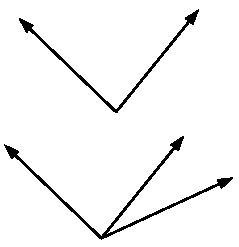
\includegraphics{part_1/chapter_2/figures/Figure1}};
		\node (x1) at (-1.7, 2.1) {$x_1$};
		\node (x2) at (1.2, 2.2) {$x_2$};
		\node (x11) at (-1.9, -0.2) {$x_1$};
		\node (x12) at (1, 0) {$x_2$};
		\node (x3) at (2.1, -0.8) {$x_3$};
    \end{tikzpicture}
	\caption{Linearly independent (top) and dependent (bottom) vectors in $\reals^2$}\label{p1c2:fig:linear_independence}
\end{figure}

Theorem \ref{p1c2:thm:fundamental_linear_algebra} summarises results that we will utilise in the upcoming developments. These are classical results from linear algebra and are thus provided without a proof.
%
\begin{theorem}[Inverses, linear independence, and solving $Ax = b$] \label{p1c2:thm:fundamental_linear_algebra}
	Let $A$ be a $m \times m$ matrix. Then, the following statements are equivalent:
	\begin{enumerate}
		\item $A$ is invertible
		\item $A^\top$ is invertible
		\item The determinant of $A$ is nonzero
		\item The rows of $A$ are linearly independent
		\item The columns of $A$ are linearly independent
		\item For every $b \in \reals^m$, the linear system $Ax = b$ has a unique solution
		\item There exists some $b \in \reals^m$ such that $Ax = b$ has a unique solution.	
	\end{enumerate}	
\end{theorem}
%
Notice that Theorem \ref{p1c2:thm:fundamental_linear_algebra} establishes important relationships between the geometry of the matrix $A$ (its rows and columns) and consequences it has to our ability to calculate its inverse $A^{-1}$ and, consequently, solve the system $Ax = b$, to which the solution is obtained as $x = A^{-1}b$. This will turn out to be most important operation in the simplex method.


\subsection{Subspaces and bases}

Let us define some objects that we will frequently refer to. The first of them is the notion of a \emph{subspace}. A subspace of $\reals^n$ is a set comprising all linear combinations of its own elements. Specifically, if $S$ is a subspace, then
%
\begin{equation*}
	S = \braces{ax + by : x,y \in S; a,b \in \reals}.
\end{equation*}
%
A related concept is the notion of a \emph{span}. A span of a collection of vectors $\braces{x_i}_{i=1}^k \in \reals^n$ is the subspace of $\reals^n$ formed by all linear combinations of such vectors, i.e., 
%
\begin{equation*}
	\spans(x_1,\dots, x_k) = \braces{y = \sum_{i=1}^k a_ix_i : a_i \in \reals, i \in \braces{1,\dots, k}}. 
\end{equation*}
%
Notice how the two concepts are related: subspaces can be characterised by a collection of vectors to which the span gives the said subspace. In other words, the span of a set of vectors is the subspace formed by all points we can represent by some linear combination of these vectors. 

The missing part in this is the notion of a \emph{basis}. A \emph{basis} of the subspace $S \subseteq \reals^n$ is a collection of vectors $\braces{x_i}_{i=1}^k \in \reals^n$ that are linearly independent such that $\spans(x_1,\dots, x_k) = S$. 

Notice that a basis is a ``minimal'' set of vectors that form a subspace. You can think of it in light of the definition of linearly independent vectors; if a vector is linearly dependent to the others, it is not needed for characterising the subspace the vectors span, since it can be represented by a linear combination of the other vectors (and thus is in the subspace formed by the span of the other vectors).

The above leads us to some important realisations:

\begin{enumerate}
	\item All bases of a given subspace $S$ have the same dimension. Any extra vector would be linearly dependent to those vectors that span $S$. In that case, we say that the subspace has size (or dimension) $k$, the number of linearly independent vectors forming the basis of the subspace.
	\item If the subspace $S \subset \reals^n$ is formed by a basis of size $m < n$, we say that $S$ is a proper subspace, because it is not the whole $\reals^n$ itself, but a space contained within $\reals^n$. For example, two linearly independent vectors form (i.e., span) a hyperplane in $\reals^3$; this hyperplane is a proper subspace since $m=2 <3=n$.
	\item If a proper subspace has dimension $m < n$, then it means that there are $n-m$ directions in $\reals^n$ that are perpendicular to the subspace and to each other. That is, there are nonzero vectors $a_i$ that are orthogonal to each other and to $S$. Or, equivalently, $a_i^\top x = 0$ for $i = n-m + 1, ..., n$. Referring to the $\reals^3$, if $m=2$, then there is a third direction that is perpendicular to (or not in) $S$. Figure \ref{p1c2:fig:proper_subpaces} illustrates this.
\end{enumerate}

\begin{figure}
	\centering
	\begin{tikzpicture}
%			\draw[help lines] (-4,-2) grid (4,2);
		\node (pic) at (0,0) {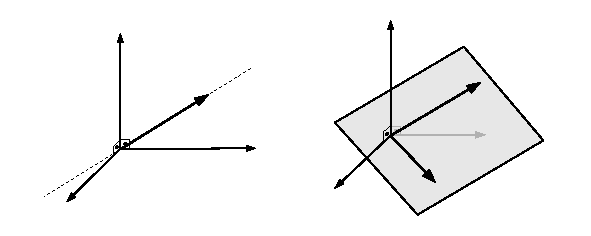
\includegraphics{part_1/chapter_2/figures/Figure2}};
		\node (x1l) at (-1.6, 0.6) {$x_1$};
		\node (Sl) at (-1.1, 0.9) {$S$};	
		\node (x1r) at (2.8, 0.8) {$x_1$};
		\node (x2r) at (2.6, -0.9) {$x_2$};
		\node (Sr) at (3.7, -0.3) {$S$};
	\end{tikzpicture}
	\vspace{-12pt}
	\caption{One- (left) and two-dimensional subspaces (right) in $\reals^3$} \label{p1c2:fig:proper_subpaces}
\end{figure}

Theorem \ref{p1c2:thm:LI_and_bases} builds upon the previous points to guarantee the existence of bases and propose a procedure to form them.

\begin{theorem}[Forming bases from linearly independent vectors]\label{p1c2:thm:LI_and_bases}
	Suppose that $S = \spans(x_1,\dots, x_k)$ has dimension $m \leq k$. Then
	\begin{enumerate}
		\item There exists a basis of $S$ consisting of $m$ of the vectors $x_1,\dots, x_k$.
		\item If $k' \leq m$ and $x_1,\dots, x_{k'} \in S$ are linearly independent, we can form a basis for $S$ by starting with $x_1,\dots, x_{k'}$ and choosing $m-{k'}$ additional vectors from $x_1,\dots, x_k$.
	\end{enumerate}	
\end{theorem}

%TODO: Include proof.

Our interest in subspaces and bases spans from (pun intended!) their usefulness in explaining how the simplex method works under a purely algebraic (as opposed to geometric) perspective. For now, we can use the opportunity to define some ``famous'' subspaces which will often appear in our derivations. 

Let $A$ be a $m \times n$ matrix as before. The \emph{column space} of $A$ consists of the subspace spanned by the $n$ columns of $A$ and has dimension $m$ (recall that each column has as many components as the number of rows and is thus a $m$-dimensional vector). Likewise, the \emph{row space} of $A$ is the subspace in $\reals^n$ spanned by the rows of $A$. Finally, the \emph{null space} of $A$, often denoted as $\nulls(A) = \braces{x \in \reals^n : Ax = 0}$, consist of the vectors that are perpendicular to the row space of $A$. 

One important notion related to those subspaces is that of their size. Both the row and the column space have the same size, and that size is the \emph{rank} of $A$. If $A$ is \emph{full rank}, than it means that 
%
\begin{equation*}
	\rank(A) = \min \braces{m,n}. 		
\end{equation*}
%
Finally, the size of the null space of $A$ is given $n - \rank(A)$, which is in line with Theorem \ref{p1c2:thm:LI_and_bases}.


\subsection{Affine subspaces}

A related concept is that of an \emph{affine subspace}. Differently from linear subspaces (to which we have been referring to simply as subspaces), affine subspaces encode some form of translation, such as  
%
\begin{equation*}
	S = S_0 + x_0 = \braces{x + x_0 : x \in S_0}.
\end{equation*}
%
Affine subspaces are not subspaces, because they do not contain the origin (recall that the definition of subspaces allows for $a$ and $b$ to be zero). Nevertheless, $S$ has the \emph{same dimension} as $S_0$.

Affine subspaces give a framework for representing linear programming problems algebraically. Specifically, let $A$ be a $m \times n$ matrix with $m < n$ (which will always be the case in linear programming models in this form as we will see) and $b$ a $m$-dimensional vector. Then, let 
%
\begin{equation} \label{p1c2:eq:equality_constraint_feasible_set}
	S = \braces{x \in \reals^n : Ax = b}.		
\end{equation}
%
As we will see, the feasible set of any linear programming problem can be represented as an equality-constrained equivalent of the form of \eqref{p1c2:eq:equality_constraint_feasible_set} by means of adding slack variables to the inequality constraints. Now, assume that $x_0 \in \reals^n$ is such that $Ax_0 = b$.  Then, we have that 
%
\begin{equation*}
	Ax = Ax_0 = b \Rightarrow A(x - x_0) = 0.	
\end{equation*}
%
Thus, $x \in S$ if and only if the vector $(x - x_0)$ belongs to $\nulls(A)$, the nullspace of $A$. Notice that the feasible region $S$ can be also defined as 
%
\begin{equation*}
	S = \braces{x + x_0 : x \in \nulls(A)},	
\end{equation*}
%
being thus an affine subspace with dimension $n-m$, if $A$ has $m$ linearly independent rows (i.e., $\rank(A)=m$). This will have important implications in the way we can define multiple basis from the $n$ vectors in the column space by choosing $m$ to be removed and form a basis to $\nulls(A)$, and what this process means geometrically.

Figure \ref{p1c2:fig:nill_space_a} illustrates this concept for a single-row matrix $a$. For multiple rows, one would see $S$ as being represented by the intersection of multiple hyperplanes.

\begin{figure}
	\begin{tikzpicture}
	    \node (pic) at (0,0) {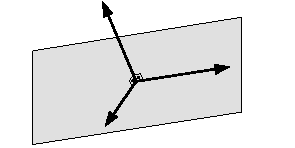
\includegraphics{part_1/chapter_2/figures/Figure3}};
	    \node (x0) at (0,-0.4) {$x_0$};
	    \node (x1) at (1.4,0.4) {$x_1$};
	    \node (x2) at (-1,-0.9) {$x_2$};
	    \node (a) at (-0.5,1.4) {$a$};
	    \node (S) at (-1.7,0.2) {$S$}; 
	\end{tikzpicture}
	\caption{The affine subspace $S$ generated by $x_0$ and $\nulls(a)$} \label{p1c2:fig:nill_space_a}		
\end{figure}


\section{Convex polyhedral set}

The feasible region of any linear programming problem is a convex polyhedral set, which we will simply refer to as a polyhedral set. That is because we are interested in polyhedral sets that are formed by an intersection of a finite number of half-spaces, and can thus only be convex (as we will see in a moment), creating redundancy in our context, but maybe some confusion overall. 

\subsection{Hyperplanes, half-spaces and polyhedral sets}

Definition \ref{p1c2:def:polyhedral_sets} formally states the structure we refer to as polyhedral sets.
%
\begin{definition}[Polyhedral set] \label{p1c2:def:polyhedral_sets}
	A polyhedral set is a set that can be described as
	$$
	S = \braces{x \in \reals^n : Ax \geq b},	
	$$
	where $A$ is an $m \times n$ matrix and $b$ is a $m$-vector.
\end{definition}
%
One important thing to notice is that polyhedral sets, as defined in Definition \ref{p1c2:def:polyhedral_sets}, as formed by the intersection multiple half-spaces. Specifically, let $\braces{a_i}_{i=1}^m$ be the rows of $A$. Then, the set $S$ can be described as 
%
\begin{equation}
	S = \braces{x \in \reals^n : a_i^\top x \geq b_i, i = 1,\dots, m}, 	
\end{equation}
%
which represents exactly the intersection of the half-spaces $a_i^\top x \geq b_i$. Furthermore, notice that the hyperplanes $a_i^\top x = b_i$, $\forall i \in \braces{1,\dots, m}$, are the boundaries of each hyperplane, and thus describe one of the faces of the polyhedral set, which is generally given by $\braces{x \in S : a_i^\top x \geq b_i}$ for a given face $i \in \braces{1,\dots, m}$. Figure \ref{p1c2:fig:hyperplanes_and_polyhedral_set} illustrates a hyperplane forming two half-spaces (also polyhedral sets) and how the intersection of five half-spaces form a (bounded) polyhedral set.

\begin{figure}[h]
			\begin{tikzpicture}
		    \node (pic) at (0,0) {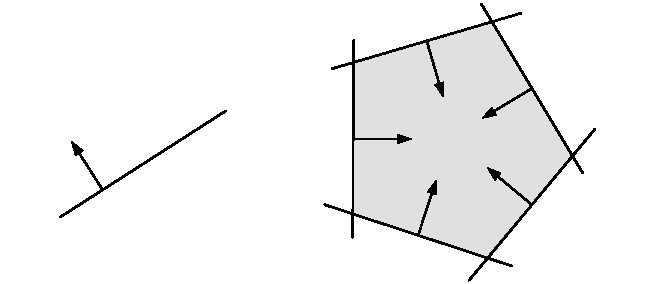
\includegraphics{part_1/chapter_2/figures/Figure4}};
		    \node (a) at (-4.5,0.2) {$a$};
			\node (ax=b) at (-3.6,-1.3) {$a^\top x =b$};
			\node (ax<b) at (-2.5, 0.8) {$a^\top x > b$};
			\node (ax>b) at (-2.3,-0.7) {$a^\top x < b$};
			\node (a1) at (1.5, -0.2) {$a_1$};
			\node (a2) at (2.8, 0.2) {$a_2$};
			\node (a3) at (1.8, 0.7) {$a_3$};
			\node (a4) at (2.9, -0.3) {$a_4$};
			\node (a5) at (2.2, -0.8) {$a_5$};
			\node[rotate = 90] (a1x=b1) at (0.1,0.2) {$a_1^\top x =b_1$};
			\node (a3x=b3) at (1.5,2.2) {$a_3^\top x =b_3$};
			\node (a2x=b2) at (4.5, 1) {$a_2^\top x =b_2$};
			\node (a4x=b4) at (4.4,-1.2) {$a_4^\top x =b_4$};
			\node (a5x=b5) at (1.3,-2) {$a_5^\top x =b_5$};
			\end{tikzpicture}
			\vspace{1pt}
		\caption{A hyperplane and its respective halfspaces (left) and the polyhedral set $\braces{x\in \reals^{2} : a_i^x \leq b_i, i =1,\dots, 5}$ (right).} \label{p1c2:fig:hyperplanes_and_polyhedral_set}		
	\end{figure}

You might finds authors referring to bounded polyhedral sets as polytopes, though this is not used consistently across references, sometimes with switched meanings (for example, using polytope to refer to a set defined as in Definition \ref{p1c2:def:polyhedral_sets} and using polyhedron to refer to a bounded version of $S$). In this text, we will only use the term polyhedral set to refer to sets defined as in Definition \ref{p1c2:def:polyhedral_sets} and use the term bounded whenever applicable.

% TODO: include a more rigorous presentation of face and facets. 


\subsection{Convexity of polyhedral sets}

As will see in more details in Part 2 of this text, convexity plays a crucial role in optimisation, being the ``watershed'' between easy and hard optimisation problems. One of the main reasons why we can solve challenging linear programming problems is due to the inherent convexity of polyhedral sets.

Let us first define the notion of convexity for sets, which is stated in Definition \ref{p1c2:def:convex_set} 

\begin{definition}[Convex set]\label{p1c2:def:convex_set} 
	A set $S \subseteq \reals^n$ is convex if, for any $x_1,x_2 \in S$ and any $\lambda \in [0,1]$, we have that $\overline{x} = \lambda x_1 + (1-\lambda) x_2 \in S$.
\end{definition}

Definition \ref{p1c2:def:convex_set} leads to a simple geometrical intuition: for a set to be convex, the line segment connecting any two points within the set must lie within the set. This is illustrated in Figure \ref{p1c2:fig:convex_sets}.

\begin{figure}
	\begin{tikzpicture}
		\node (pic) at (0,0) {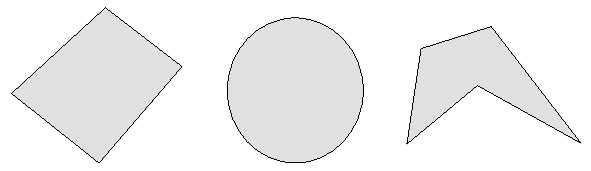
\includegraphics{part_1/chapter_2/figures/Figure5}};
		% Left pic line
		\node[circle, fill, minimum size=3pt, inner sep = 0pt] (x1) at (-4,-0.5) {};
		\node[above left] at (-4,-0.5) {$x_1$};
		\node[circle, fill, minimum size=3pt, inner sep = 0pt] (x2) at (-2.8,0.5) {};
		\node[above left] at (-2.8,0.5) {$x_2$};
		\draw[thick] (x1) -- (x2);
		% Center pic line
		\node[circle, fill, minimum size=3pt, inner sep = 0pt] (x1) at (-0.5,-0.5) {};
		\node[above left] at (-0.5,-0.5) {$x_1$};
		\node[circle, fill, minimum size=3pt, inner sep = 0pt] (x2) at (0.5,0.5) {};
		\node[above left] at (0.5,0.5) {$x_2$};
		\draw[thick] (x1) -- (x2);
		\node[circle, fill, minimum size=3pt, inner sep = 0pt] (x1) at (2.3, -0.3) {};
		\node[above] at (2.3, -0.3) {$x_1$};
		\node[circle, fill, minimum size=3pt, inner sep = 0pt] (x2) at (4,-0.3) {};
		\node[above left] at (4,-0.3) {$x_2$};
		\draw[thick] (x1) -- (x2);
	\end{tikzpicture}
	\caption{Two convex sets (left and middle) and one nonconvex set (right)} \label{p1c2:fig:convex_sets}
\end{figure}

Associated with the notion of convex sets are two important elements we will refer to later, when we discuss linear problems that embed \emph{integrality requirements}. The first is the notion of a convex combination, which is already contained in Definition \ref{p1c2:def:convex_set}, but can be generalised for an arbitrary number of points. The second consists of \emph{convex hulls}, which are sets formed by combining the convex combinations of all elements within a given set. As one might suspect, convex hulls are always convex sets, regardless whether the original set from which the points are drawn from is convex or not. These are formalised in Definition \ref{p1c2:def:convex_combination_hull} and illustrated in Figure \ref{p1c2:fig:convex_hulls}.

\begin{definition}[Convex combinations and convex hulls] \label{p1c2:def:convex_combination_hull}
	Let $x_1, \dots, x_k \in \reals^n$ and $\lambda_1,\dots, \lambda_k \in \reals$ such that $\lambda_i \geq 0$ for $i = 1, \dots, k$ and $\sum_{i=1}^k \lambda_i = 1$. Then
	\begin{enumerate}
		\item $x = \sum_{i=1}^k \lambda_i x_i$ is a \emph{convex combination} of $\braces{x_i}_{i=1}^k \in \reals^n$.
		\item The \emph{convex hull} of $\braces{x_i}_{i=1}^k \in \reals^n$, denoted $\conv(x_1, \dots, x_k)$, is the set of all convex combinations of $\braces{x_i}_{i=1}^k \in \reals^n$.
	\end{enumerate}		
\end{definition}

\begin{figure}
	\begin{tikzpicture}
		\node (pic) at (0,0) {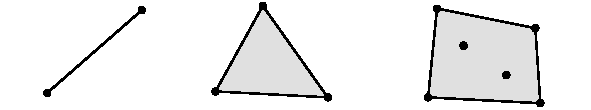
\includegraphics{part_1/chapter_2/figures/Figure6}};
		\node (x1l) at (-4.5,-0.7) {$x_1$};
		\node (x2l) at (-2.3, 0.7) {$x_2$};
		\node (x1c) at (-0.5, 1.1) {$x_1$};
		\node (x2c) at (0.8, -1) {$x_2$};
		\node (x3c) at (-1.5, -0.9) {$x_3$};
		\node (x1r) at (2.1, 1) {$x_1$};
		\node (x2r) at (4.4, 0.6) {$x_2$};
		\node (x3r) at (4.5, -0.9) {$x_3$};
		\node (x4r) at (1.9, -0.9) {$x_4$};
		\node (x5r) at (2.7, 0.4) {$x_5$};
		\node (x6r) at (3.8, -0.15) {$x_6$};
	\end{tikzpicture}
	\vspace{-6pt}
	\caption{The convex hull of two points is the line segment connecting them (left); The convex hull of three (centre) and six (right) points in $\reals^2$} \label{p1c2:fig:convex_hulls}
\end{figure}	

We are now ready to state the result that guarantees the convexity of polyhedral sets of the form
$$
	S = \braces{x \in \reals^n : Ax \le b}.
$$


\begin{theorem}[Convexity of polyhedral sets] \label{p1c2:thm:convexity}
	The following statements are true:
	\begin{enumerate}
		\item The intersection of convex sets is convex
		\item Every polyhedral set is a convex set
		\item A convex combination of a finite number of elements of a convex set also belongs to that set
		\item The convex hull of a finite number of elements is a convex set.			
	\end{enumerate}
\end{theorem}

\begin{proof}
	We provide proofs to each of the statements individually. 
	\begin{enumerate}
	 \item Let 	$S_i$, for $i \in I$, be convex sets and suppose that $x, y \in \bigcap_{i \in I} S_i$. Let $\lambda \in [0,1]$. Since $S_i$ are convex and $x,y \in S_i$ for all $i \in I$, $\lambda x + (1-\lambda) y \in S_i$ for all $i \in I$ and, thus, $\lambda x + (1-\lambda) y \in \bigcap_{i \in I} S_i$.
	
	\item Let $a \in \reals^n$ and $b \in \reals$. Let $x,y \in \reals^n$, such that $a^\top x \geq b$ and $a^\top y \geq b$. Let $\lambda \in [0,1]$. Then $a^\top (\lambda x + (1-\lambda)y) \geq \lambda b + (1-\lambda)b = b$, showing that half-spaces are convex. The result follows from combining this with (1).    
	
	\item By induction. Let $S$ be a convex set and assume that the convex combination of $x_1, \dots, x_k \in S$ also belongs to $S$. Consider $k+1$ elements $x_1, \dots, x_{k+1} \in S$ and $\lambda_1, \dots, \lambda_{k+1}$ with $\lambda_i \in [0,1]$ for $i = 1,\dots, k+1$ and $\sum_{i=1}^{k+1}\lambda_i = 1$ and $\lambda_{k+1} \neq 1$ (without loss of generality). Then

	\begin{equation}
		\sum_{i=1}^{k+1}\lambda_i x_i = \lambda_{k+1}x_{k+1} + (1 - \lambda_{k+1}) \sum_{i=1}^k \frac{\lambda_i}{1 - \lambda_{k+1}}x_i. \label{p1c2:eq:induction}
	\end{equation}								

		Notice that $\sum_{i=1}^{k}\frac{\lambda_i}{1 - \lambda_{k+1}} = 1$. Thus, using the induction hypothesis, $\sum_{i=1}^{k}\frac{\lambda_i}{1 - \lambda_{k+1}}x_i \in S$. Considering that $S$ is convex and using \eqref{p1c2:eq:induction}, we conclude that $\sum_{i=1}^{k+1}\lambda_{k+1}x_{k+1} \in S$, completing the induction.
		
	\item Let $S = \conv(x_1, \dots, x_k)$. Let $y = \sum_{i=1}^k \alpha_i x_i$ and $z = \sum_{i=1}^k \beta_ix_i$ be such that $y,z \in S$, $\alpha_i,\beta_i \geq 0$, and $\sum_{i=1}^k \alpha_i = \sum_{i=1}^k \beta_i = 1$. Let $\lambda \in [0,1]$. Then
		%
		\begin{equation}
			\lambda y + (1- \lambda)z = \lambda\sum_{i=1}^k \alpha_i + (1-\lambda)\sum_{i=1}^k \beta_i = \sum_{i=1}^k (\lambda \alpha_i + (1-\lambda) \beta_i)x_i. 	
		\end{equation}
		%
		Since $\sum_{i=1}^k \lambda \alpha_i + (1-\lambda) \beta_i = 1$ and $\lambda \alpha_i + (1-\lambda) \beta_i \geq 0$ for $i=1,\dots,k$, $\lambda y + (1- \lambda)z$ is a convex combination of $x_1, \dots, x_k$ and, thus, $\lambda y + (1- \lambda)z \in S$, showing the convexity of $S$. \qedhere	
	\end{enumerate}	
\end{proof}

Figure \ref{p1c2:fig:convexity_theorem_examples} illustrates some of the statements represented in the proof. For example, the intersection of the convex sets is always a convex set. One should notice however that the same does not apply to the union of convex sets. Notice that statement 2 proves that polyhedral sets as defined according to Definition \ref{p1c2:def:polyhedral_sets} are convex. Finally the third figure on the right illustrates the convex hull of four points as a convex polyhedral set containing the lines connecting any two points within the set. 
 
\begin{figure}
	\begin{tikzpicture}
%			\draw[help lines] (-5,-1) grid (5,1);
		\node (pic) at (0,0) {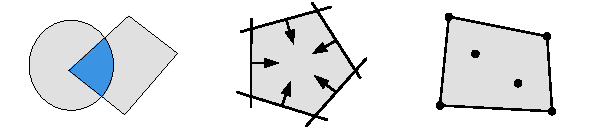
\includegraphics{part_1/chapter_2/figures/Figure7}};
	\end{tikzpicture}
    \vspace{-6pt}
	\caption{Illustration of statement 1 (left), 2 (centre), and 3 and 4 (right)} \label{p1c2:fig:convexity_theorem_examples}
\end{figure}	

We will halt our discussion about convexity for now and return to it in deeper details in Part 2. As it will become clearer then, the presence of convexity (which is a given in the context of linear programming, as we have just seen) is what allows us to conclude that the solutions returned by our optimisation algorithms are indeed optimal for the problem at hand. 


\section{Extreme points, vertices, and basic feasible solutions}

Now we focus on the algebraic representation of the most relevant geometric elements in the optimisation of linear programming problems. As we have seen in the graphical example in the previous chapter, the optimum of linear programming problems is generally located at the vertices of the feasible set. Furthermore, such vertices are formed by the intersection of $n$ constraints (in $n$-dimensional space, which comprises constraints that are active (or satisfied at the boundary of the half-space of said constraints).

First, let us formally define the notions of vertex and extreme point. Though in general these can refer to different objects, we will see that in the case of linear programming problems, if a point is a vertex, then it is an extreme point as well, being the converse also true.

\begin{definition}[Vertex] \label{p1c2:def:vertex}
	Let $P$ be a convex polyhedral set. The vector $x \in P$ is a vertex of $P$ if there exists some $c$ such that $c^\top x < c^\top y$ for all $y \in P$ with $y \neq x$.
\end{definition}

\begin{definition}[Extreme points]\label{p1c2:def:extreme_point}
	Let $P$ be a convex polyhedral set. The vector $x \in P$ is an extreme point of $P$ if there are no two vectors $y,z \in P$ (different than $x$) such that $x = \lambda y + (1 - \lambda)z$, for any $\lambda \in [0,1]$.
\end{definition}

Figure \ref{p1c2:fig:vertex_and_extreme_point} provides an illustration of the Definitions \ref{p1c2:def:vertex} and \ref{p1c2:def:extreme_point}. Notice that, while the definition of a vertex involves an additional hyperplane that, once placed on a vertex point, strictly contains the whole polyhedral set in one of the half-spaces it defines, with the exception of the vertex itself. On the other hand, the definition of an extreme point only relies on convex combinations of elements in the set itself. 

\begin{figure}
	\begin{tikzpicture}
		\node (pic) at (0,0) {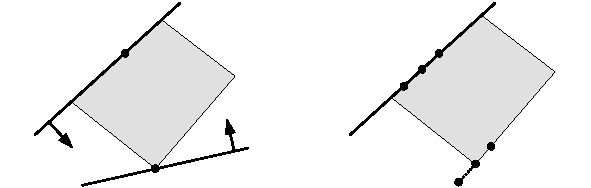
\includegraphics{part_1/chapter_2/figures/Figure8}};
		\node (Pl) at (-2.5, 0) {$P$};
		\node (Pr) at (3, 0) {$P$};
		\node (wl) at (-3, 0.9) {$w$};
		\node (xl) at (-2.3, -1.5) {$x$};
		\node (c1) at (-4, -1) {$c$};
		\node (c2) at (-0.9, -0.5) {$c$};
		\node[left] (cw) at (-2.3, 1.5) {$\braces{y : c^\top y = c^\top w}$};
		\node[right] (cx) at (-1.7, -1.4) {$\braces{y : c^\top y = c^\top x}$};
		\node (wr) at (2.1, 0.7) {$w$};
		\node (vr) at (2.4, 0.9) {$v$};
		\node (ur) at (1.8, 0.4) {$u$};
		\node (xr) at (3.1, -1.5) {$x$};
		\node (yr) at (3.4, -1.2) {$y$};
		\node (zr) at (2.8, -1.8) {$z$};
	\end{tikzpicture}
	\caption{Representation of a vertex (left) and a extreme point (right)} \label{p1c2:fig:vertex_and_extreme_point}
\end{figure}	

Now we focus on the description of active constraints under an algebraic standpoint. For that, let us first generalise our setting by considering all possible types of linear constraints. That is, let us consider the convex polyhedral set $P \subset \reals^n$, formed by the set of inequalities and equalities:
%
\begin{align*}
	& a_i^\top x \geq b, i \in M_1, \\ 
	& a_i^\top x \leq b, i \in M_2, \\
	& a_i^\top x = b, i \in M_3.
\end{align*}

Definition \ref{p1c2:fig:active_constraint} formalises the notion of active constraints. This is illustrated in Figure \ref{p1c2:fig:active_constraints}, where the polyhedral set $P = \braces{x \in \reals^3 : x_1 + x_2 + x_3 = 1, x_i \geq 0, i =1,2,3}$ is represented. Notice that, while points $A$, $B$, $C$ and $D$ have 3 active constraints, $E$ only has 2 active constraints ($x_2 = 0$ and $x_1 + x_2 + x_3 = 1$).

\begin{definition}[Active (or binding) constraints] \label{p1c2:fig:active_constraint}
	If a vector $\overline{x}$ satisfies $a_i^\top \overline{x} = b_i$ for some $i \in M_1, M_2$, or $M_3$, we say that the corresponding constraints are active (or binding).
\end{definition}

\begin{figure}[h]
	\begin{tikzpicture}
		\node (pic) at (0,0) {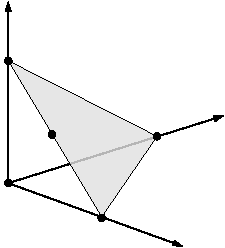
\includegraphics{part_1/chapter_2/figures/Figure9}};
		\node (x1) at (1.5, -2) {$x_1$};
		\node (x2) at (1.7, 0.4) {$x_2$};
		\node (x3) at (-2.1, 2) {$x_3$};
		\node (P) at (0, -0.5) {$P$};
		\node[left] (A) at (-1.1, 1.3) {$A$};
		\node[left] (B) at (-1.8, -1) {$B$};
		\node[right] (C) at (-0.5, -1.9) {$C$};
		\node[above] (D) at (0.9, -0.1) {$D$};
		\node[right] (E) at (-1.6, -0.2) {$E$};
	\end{tikzpicture}
	\caption{Representation of $P$ in $\reals^3$.} \label{p1c2:fig:active_constraints}
\end{figure}	


Theorem \ref{p1c2:thm:active_const} sows a thread between having a collection of active constraints forming a vertex and being able to describe it as a basis of a subspace that is formed by the vectors $a_i$ that form these constraints. This link is what will allow us to characterise vertices by their forming active constraints.

\begin{theorem}[Properties of active constraints]\label{p1c2:thm:active_const}
	Let $\overline{x} \in \reals^n$ and $I = \braces{ i \in M_1 \cup M_2 \cup M_3 \mid a_i^\top \overline{x} = b_i}$. Then, the following are equivalent:
	\begin{enumerate}
		\item There exists $n$ vectors in $\braces{a_i}_{i \in I}$ that are linearly independent.  
		\item The $\spans(\braces{a_i}_{i \in I})$ spans $\reals^n$. That is, every $x \in \reals^n$ can be expressed as a linear combination of $\braces{a_i}_{i \in I}$.
		\item The system of equations $\braces{a_i ^\top x = b_i}_{i \in I}$ has a unique solution.
	\end{enumerate}
\end{theorem}

\begin{proof}
	Suppose that $\braces{a_i}_{i \in I}$ spans $\reals^n$, implying that the $\spans(\braces{a_i}_{i \in I})$ has dimension $n$. By Theorem \ref{p1c2:thm:LI_and_bases} (part 1), $n$ of these vectors form a basis for $\reals^n$ and are, thus, linearly independent. Moreover, they must span $\reals^n$ and therefore every $x \in \reals^n$ can be expressed as a combination of $\braces{a_i}_{i \in I}$. This connects (1) and (2).
	
	Assume that the system of equations $\braces{a_i ^\top x = b_i}_{i \in I}$ has multiple solutions, say $x_1$ and $x_2$. Then, the nonzero vector $d = x_1 - x_2$ satisfies $a_i^\top d = 0$ for all $i \in I$. As $d$ is orthogonal to every $a_i$, $i \in I$, $d$ cannot be expressed as a combination of $\braces{a_i}_{i \in I}$ and, thus, $\braces{a_i}_{i \in I}$ do not span $\reals^n$.
	
	Conversely, if $\braces{a_i}_{i \in I}$ do not span $\reals^n$, choose $d \in \reals^n$ that is orthogonal to $\spans(\braces{a_i}_{i \in I})$. If $x$ satisfies $\braces{a_i ^\top x = b_i}_{i \in I}$, so does $\braces{a_i ^\top (x + d) = b_i}_{i \in I}$, thus yielding multiple solutions. This connects (2) and (3). \qedhere
\end{proof}

Notice that Theorem \ref{p1c2:thm:active_const} implies that there are (at least) \emph{$n$ active constraints ($a_i$)} that are \emph{linearly independent} at $\overline{x}$. This is the reason why we will refer to $\overline{x}$ and any vertex forming solution a \emph{basic solution}, of which we will be interested in those that are feasible, i.e., that satisfy all constraints $i \in M_1 \cup M_2 \cup M_3$. Definition \ref{p1c2:def:basic_feasible_solution} provides a formal definition of these concepts.

\begin{definition}[Basic feasible solution (BFS)] \label{p1c2:def:basic_feasible_solution}
	Consider a convex polyhedral set $P \subset \reals^n$ defined by linear equality and inequality constraints, and let $\overline{x} \in \reals^n$.
	\begin{enumerate}
		\item $\overline{x}$ is a \emph{basic solution} if 
		\begin{enumerate}
			\item All equality constraints are active and,
			\item Out of the constraints active at $\overline{x}$, $n$ of them are linearly independent.
		\end{enumerate}
		\item if $\overline{x}$  is a basic solution satisfying all constraints, we say $\overline{x}$ is a basic feasible solution. 
	\end{enumerate}
\end{definition}

Figure \ref{p1c2:fig:BFS} provides an illustration of the notion of basic solutions, and show how only a subset of the basic solutions are feasible. As one might infer, these will be the points of interest in out future developments, as these are the candidates for optimal solution.

\begin{figure}[h]
	\begin{tikzpicture}
		\node (pic) at (0,0) {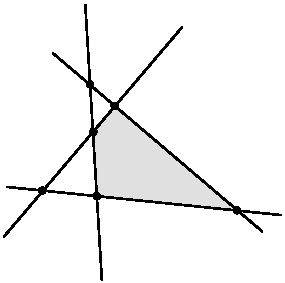
\includegraphics{part_1/chapter_2/figures/Figure10}};
		\node[above] (A) at (-0.7, 1) {$A$};
		\node[left] (B) at (-0.9, 0.2) {$B$};
		\node[right] (C) at (-0.4, 0.7) {$C$};
		\node[below] (D) at (1.6, -1.2) {$D$};
		\node[below] (E) at (-0.5, -1) {$E$};
		\node[above] (F) at (-1.8, -0.8) {$F$};
		\node (P) at (-0.3, -0.3) {$P$};
	\end{tikzpicture}
	\caption{Points $A$ to $F$ are basic solutions; $B$,$C$,$D$, and $E$ are BFS.} \label{p1c2:fig:BFS}
\end{figure}		

We finalise stating the main result of this chapter, which formally confirms the intuition we developed so far. That is, for convex polyhedral sets, the notion of vertices and extreme points coincide and these points can be represented as basic feasible solutions. This is precisely the link that allows to treat the feasible region of linear programming problems under a purely algebraic characterisation of the candidates for optimal solutions, those described uniquely by a subset of constraints of the problem.

\begin{theorem}[BFS, extreme points and vertices]\label{p1c2:thm:BFS_vertex_extreme_point}
	Let $P \subset \reals^n$ be a convex polyhedral set and let $\overline{x} \in P$. Then, the following are equivalent
	$$	\overline{x} \text{ is a vertex} \iff \overline{x} \text{ is an extreme point} \iff \overline{x} \text{ is a BFS}.	
	$$
\end{theorem}


\begin{proof}
	Let $P =\{ x \in \reals^n \mid a_i^\top x \geq b_i, i \in M_1, a_i^\top x = b_i, i \in M_2\}$, and $I = \braces{i \in M_1 \cup M_2 \mid a_i^\top x = b_i}$.
	
	\begin{enumerate}
		\item (Vertex $\Rightarrow$ Extreme point) Suppose $\overline{x}$ is a vertex. Then, there exists some $c \in \reals^n$ such that $c^\top\overline{x} < c^\top x$, for every $x \in P$ with $x \neq \overline{x}$ (cf. Definition \ref{p1c2:def:vertex}). Take $y,z \in P$ with $y,z \neq \overline{x}$. Thus $c^\top\overline{x} < c^\top y$ and $c^\top\overline{x} < c^\top z$. For $\lambda \in [0,1]$, $c^\top \overline{x} < c^\top(\lambda y + (1-\lambda)z)$ implying that $\overline{x} \neq \lambda y + (1-\lambda)z$, and is thus an extreme point (cf. Definition \ref{p1c2:def:extreme_point}).
		
		\item (Extreme point $\Rightarrow$ BFS) suppose $\overline{x} \in P$ is not a BFS. Then, there are no $n$ linearly independent vectors within $\braces{a_i}_{i \in I}$. Thus $\braces{a_i}_{i \in I}$ lie in a proper subspace of $\reals^n$. Let the nonzero vector $d \in \reals^n$ be such that $a_i^\top d = 0$, for all $i \in I$.
			
			Let $\epsilon > 0$, $y = \overline{x} + \epsilon d$, and $z = \overline{x} - \epsilon d$. Notice that $a_i^\top y = a_i^\top z = b_i$, for all $i \in I$. Moreover, for $i \neq I$, $a_i^\top x > b$ and, provided that $\epsilon$ is sufficiently small (such that $\epsilon|a_i^\top d| < a_i ^\top \overline{x} - b_i $), we have that $a_i ^\top x \geq b_i$. Thus $y \in P$, and by a similar argument, $z \in P$. Now, by noticing that $\overline{x} = \frac{1}{2}y + \frac{1}{2}z$, we see that $\overline{x}$ is not an extreme point. 			 
		\item (BFS $\Rightarrow$ Vertex) Let $\overline{x}$ be a BFS. Define $c = \sum_{i \in I} a_i$. Then
			\begin{equation*}
				c^\top \overline{x} = \linebreak \sum_{i \in I} a_i^\top \overline{x} = \sum_{i \in I} b_i.	 			 	
	 		\end{equation*}
			Also, for any $x \in P$, we have that 
			\begin{equation*}
				c^\top x = \sum_{i \in I} a_i^\top x \geq \sum_{i \in I} b_i, 	 	
	 		\end{equation*}
	 		since $a_i^\top x \geq b_i$ for $i \in M_1 \cup M_2$. Thus, for any $x \in P$, $c^\top \overline{x} \leq c^\top x$, making $\overline{x}$ a vertex (cf. Definition \ref{p1c2:def:vertex}). \qedhere
	\end{enumerate} 	
\end{proof}

Some interesting insights emerge from the proof of Theorem \ref{p1c2:thm:BFS_vertex_extreme_point}, upon which we will build our next developments. First, notice how the definition of vertex encodes a concept of optimality, since it implies that $\overline{x}$ is a unique minimiser (i.e., all other feasible points $y$ are such that $c^\top\overline{x} < c^\top y$). Also, once the relationship between being a vertex/ extreme point and a BFS is made, it means that $\overline{x}$ can be recovered as the unique solution of a system of linear equations, these equations being the active constraints at that vertex. This means that the list of all candidate points for optimal solution can be obtained by simply looking at all possible combinations of $n$ active constraints, discarding those that are infeasible. This means that the number of candidates for optimal solution is \emph{finite} and can be bounded by $\binom{m}{n}$, where $m=| M_1 \cup M_2 |$. 


\section{Exercises}

\subsection*{Exercise 2.1: Polyhedral sets}
Which of the following sets are polyhedral?
\begin{itemize}
\item[(a)] $\{(x,y)\in\mathbb{R}^2~|~ x \cos \theta + y\sin\theta \leq 1,\theta\in[0,\pi/2],x\geq0,y\geq0\}$
\item[(b)] $\{x\in\mathbb{R}~|~ x^2-8x+15\leq 0\}$
\item[(c)] The empty set ($\emptyset$).
\end{itemize}

\subsection*{Exercise 2.2: Convexity of polyhedral sets}
Prove the following theorem.

\begin{theorem*}[Convexity of polyhedral sets] 
	%	\vspace{-3pt}
	\emph{The following convexity properties about convex sets can be said:}
	\begin{enumerate}
		\item The intersection of convex sets is convex
		\item Every polyhedral set is a convex set
		\item A convex combination of a finite number of elements of a convex set is also belongs to that set
		\item The convex hull of a finite number of elements is a convex set.			
	\end{enumerate}
\end{theorem*}

Note: the theorem is proved in the notes. Use this as an opportunity to revisit the proof carefully, and try to take as many steps without consulting the text as you can. This is a great exercise to help you internalise the proof and its importance in the context of the material. I strongly advise against blindly memorising it, as I suspect you will never (in my courses, at least) be requested to recite the proof literally.


\subsection*{Exercise 2.3: Properties of active constraints}
Let us consider the convex polyhedral set $P \subset \reals^n$, formed by the set of equalities and inequalities:
%
\begin{align*}
	a_i^\top x \geq b, i \in M_1, \\
	a_i^\top x \leq b, i \in M_2, \\
	a_i^\top x = b, i \in M_3.
\end{align*}
%

Prove the following result.

\begin{theorem*}[Properties of active constraints]
	Let $\overline{x} \in \reals^n$ and $I = \braces{ i \in M_1 \cup M_2 \cup M_3 \mid a_i^\top \overline{x} = b_i}$. Then, the following are equivalent:
	\begin{enumerate}
		\item There exists $n$ vectors in $\braces{a_i}_{i \in I}$ that are linearly independent.  
		\item The $\spans(\braces{a_i}_{i \in I})$ spans $\reals^n$. That is, every $x \in \reals^n$ can be expressed as a combination of $\braces{a_i}_{i \in I}$.
		\item The system of equations $\braces{a_i ^\top x = b_i}_{i \in I}$ has a unique solution.
	\end{enumerate}
\end{theorem*}

Note: see Exercise 2.2.

\subsection*{Exercise 2.4: Vertex, extreme points, and BFSs}
Prove the following result.

\begin{theorem*}[BFS, extreme points and vertices]
	Let $P \subset \reals^n$ be a convex polyhedral set and let $\overline{x} \in P$. Then, the following are equivalent
	\begin{enumerate}
		\item $\overline{x}$ is a vertex;
		\item $\overline{x}$ is a extreme point;
		\item $\overline{x}$ is a BFS;	
	\end{enumerate}
\end{theorem*}

Note: see Exercise 2.2.

\subsection*{Exercise 2.5: Binding constraints applications} 
Given the linear program defined by the system of inequalities below,

\begin{center}
	\begin{enumerate}
		\begin{tabular}{*4c}
			$\max$ & $2x_1 + x_2$ & \\
			s.t. \\
			& $2x_1 + 2x_2$ & $\leq$ & $9$  \\
			& $2x_1 -  x_2$ & $\leq$ & $3$  \\
			& $ x_1 -  x_2$ & $\leq$ & $1$  \\
			& $x_1$         & $\leq$ & $2.5$\\
			& $x_2$         & $\leq$ & $4$  \\
			\\
			\multicolumn{4}{c}{$x_1, x_2 \geq 0$}\\
		\end{tabular}
	\end{enumerate}
\end{center}

\noindent assess the following points relative to the polyhedron defined in $\reals^2$ by this system and classify them as in $(i)$ belonging to which active constraint(s), $(ii)$ being a non-feasible/basic/basic feasible solution, and $(iii)$ being an extreme point, vertex, or outside the polyhedron. Use Theorem \ref{p1c2:thm:active_const} and Theorem \ref{p1c2:thm:BFS_vertex_extreme_point} to check if your classification is correct.

\begin{itemize}
	\item[(a)] $(1.5,0)$
	\item[(b)] $(1,0)$
	\item[(c)] $(2,1)$
	\item[(d)] $(1.5,3)$
\end{itemize}

 


	
	\chapter{Basis, Extreme Points and Optimality in Linear Programming}
	\section{Polyhedral sets in standard form}

In the context of linear programming problems, we will often consider problems written in the so-called \emph{standard form}. The standard form can be understood as posing the linear programming problem as an under determined system of equations (that is, with less equations than variables). Then, we will work selecting subset of the variables to be set the zero, on a way that the number of remaining variables is the same as that of equations, making the system solvable. 

A key point in this chapter will be devising how we relate this process of selecting variables with that of selecting a subset of active constraints (forming a vertex, as we seen in the previous chapter) that might lead to an optimal solution. 


\subsection{The standard form of linear programming problems}

First, let us formally define the notion of a standard form polyhedral set. Let $A$ is a $m \times n$ matrix and $b \in \reals^m$. The \emph{standard form} polyhedral set $P$ is given by 
%
\begin{equation*}
	P = \braces{x \in \reals^n : Ax = b, x \geq 0}.		
\end{equation*}
%
We assume that the $m$ equality constraints are linearly independent, i.e., $A$ is full (row) rank ($m \leq n$). we know that a basic solution can be obtained from a collection of $n$ active constraints, since the problem is defined in $\reals^n$. 

One important point, to which we will return later is that \emph{any} linear programming problem can be represented in the standard form. This is achieved by means of including nonnegative \emph{slack variables}. Thus, a feasibility set that is, say, originally represented as
%
\begin{equation*}
	P = \braces{x \in \reals^n : A_1 x \le b_1, A_2x \ge b_2, x \ge 0}
\end{equation*}
%
can be equivalently represented as a standard-form polyhedral set. For that, it must be modified to consider slack variables $s_1 \ge 0$ and $s_2 \geq 0$ such that
%
\begin{equation*}
	P = \braces{(x, s_1, s_2) \in \reals^{(n + |b_1| + ||b_2)} : A_1 x + s_1 = b_1, A_2x - s_2 = b_2, (x, s_1, s_2) \ge 0},
\end{equation*}
%
where $|\cdot|$ represents the cardinality of $\cdot$. This transformation, as we will see, will be a requirement for employing the simplex method to solve linear programming problems with inequality constraints and, inevitably, will always render standard form linear programming problems with $m < n$.

The standard-form polyhedral set $P$ always has by definition $m$ active constraints, because they are its forming equality constraints. To reach the total of $n$ active constraints, $n-m$ of the remaining constraints $x_i \ge 0$, $i =1,\dots, n$ must be activated, and this is achieved by selecting $n-m$ of those to be set as $x_i = 0$. These $n$ active constraints (the original $m$ plus the $n-m$ variables set to zero) for a basic solution, as we seen in the last chapter. If it happens that the $m$ equalities can still be satisfied while the constraints $x_i \ge 0$, $i =1,\dots, n$ are satisfied, then we have a basic feasible solution.

Theorem \ref{p1c3:thm:LI_and_bases} summarises this process, guaranteeing that the setting of $n-m$ variables to zero will render a basic solution.

\begin{theorem}[Linear independence and basic solutions] \label{p1c3:thm:LI_and_bases}
	Consider the constraints $Ax = b$ and $x \geq 0$, and assume that $A$ has $m$ LI rows $M = \braces{1,\dots,m}$. A vector $\overline{x} \in \reals^n$ is a basic solution if and only if we have that $A \overline{x} = b$ and there exists indices $B(1), \dots, B(m)$ such that
	\begin{enumerate}
		\item The columns $A_{B(1)}, \dots, A_{B(m)}$ of $A$ are LI
		\item If $j \neq B(1), \dots, B(m)$, then $\overline{x}_j = 0$.
	\end{enumerate} 
\end{theorem}

\begin{proof}
	Assume that (1) and (2) are satisfied. Then the active constraints $\overline{x}_j = 0$ for $j \notin \braces{B(1), \dots, B(m)}$ and $Ax = b$ imply that
%	
	\begin{equation*}
		\sum_{i=1}^m A_{B(i)}\overline{x}_{B(i)} = \sum_{j=1}^n A_j\overline{x}_j = A\overline{x} = b.
	\end{equation*}
%
	Since the columns $\braces{A_{B(i)}}_{i \in M}$ are LI, $\braces{\overline{x}_{B(i)}}_{i \in M}$ are uniquely determined and thus $A\overline{x} = b$ has a unique solution, implying that $\overline{x}$ is a basic solution (cf. Theorem \ref{p1c2:thm:BFS_vertex_extreme_point}).
	
	Conversely, assume that $\overline{x}$ is a basic solution. Let $\overline{x}_{B(1)}, \dots, \overline{x}_{B(k)}$ be the nonzero components of $\overline{x}$. Thus, the system 
%	
		\begin{equation*}
			\sum_{i=1}^n A_i\overline{x}_i = b \text{ and } \braces{\overline{x}_i = 0}_{i \notin \braces{B(1), \dots, B(k)}}
		\end{equation*}
%
	has a unique solution, and so does $\sum_{i=1}^k A_{B(i)}\overline{x}_{B(i)} = b$, implying that the columns $A_{B(1)}, \dots, A_{B(k)}$ are linearly independent (LI). Otherwise, there would be scalars $\lambda_1,\dots, \lambda_k$, not all zeros, for which $\sum_{i=1}^k A_{B(i)}\lambda_i = 0$; this would imply that $\sum_{i=1}^k A_{B(i)}(\overline{x}_{B(i)} + \lambda_i) =b$, contradicting the uniqueness of $\overline{x}$.
	Since $A_{B(1)}, \dots, A_{B(k)}$ are LI, $k \leq m$. Also, since $A$ has $m$ LI rows, it must have $m$ LI columns spanning $\reals^m$. Using Theorem \ref{p1c2:thm:LI_and_bases}, we can obtain $m-k$ additional columns $A_{B(k+1)}, \dots, A_{B(m)}$ so that $A_{B(1)}, \dots, A_{B(m)}$ are LI. 
	
	Finally, since $k \leq m $, $\braces{\overline{x}_j = 0}_{i \notin \braces{B(1), \dots, B(m)}} \subset  \braces{\overline{x}_j = 0}_{i \notin \braces{B(1), \dots, B(k)}}$, satisfying (1) and (2). \qedhere 		
\end{proof}	

This proof highlights an important aspect in the process of generating basic solutions. Notice that, once we set $n-m$ variables to be zero, the system of equations forming $P$ becomes uniquely determined, i.e., 
%
\begin{equation*}
	\sum_{i=1}^m A_{B(i)}\overline{x}_{B(i)} = \sum_{j=1}^n A_j\overline{x}_j = A\overline{x} = b.
\end{equation*}	
%


\subsection{Forming basis for standard-form linear programming problems}

Theorem \ref{p1c3:thm:LI_and_bases} allows to develop a simple procedure to generate all basic solutions of a linear programming problem in standard form.

\begin{enumerate}
	\item Choose $m$ LI columns $A_{B(1)}, \dots, A_{B(m)}$;
	\item Let $x_j = 0$ for all $j \notin \braces{B(1), \dots, B(m)}$;
	\item Solve the system $Ax = b$ to obtain $x_{B(1)}, \dots, x_{B(m)}$.
\end{enumerate}

Perhaps it is worth pointing out something that often causes confusion at this point. You might have notice that in the proof of Theorem \ref{p1c3:thm:LI_and_bases}, the focus shifted to the columns of $A$ rather than its rows. The reason for that is because, when we think of solving the system $Ax = b$, what we are truly doing is finding a vector $x$ representing the linear combination of the columns of $A$ that yield the vector $b$. This creates an association between the columns of $A$ and the components of $x$ (i.e., the variables). 

You will notice that from here onwards we will implicitly refer to the columns of $A$ as variables. Then, when we say that we are setting some ($n-m$) of the variables to be zero, it means that we are ignoring the respective columns (the mapping between variables and columns being their indices: $x_1$ referring to the first column, $x_2$ to the second, and so forth), while using the remainder to form a (unique) combination that yields the vector $b$, being the weights of this combination precisely the solution $x$, which in turn represent the coordinates in $\reals^n$ of the vertex formed by the $n$ ($m$ equality constrains plus $n-m$ variables set to zero) active constraints.   

As we will see, this procedure will be at the core of the simplex method. Since we will be often referring to elements associated with this procedure, it will be useful to define some nomenclature.

We say that $\braces{A_{B(i)}}_{i \in I_B}$ is a \emph{basis} (or, perhaps more precisely, a basic matrix) with basic indices $I_B = \braces{B(1), \dots, B(m)}$. Consequently, we say that the variables $x_j$, for $x_j$, for $j \in I_B$, are \emph{basic variables}. Somewhat analogously, we say that the variables chosen to be set to zero are the \emph{nonbasic variables} $x_j$, for $j \in I_N$, where $I_N = J \setminus I_B$, with $J = \braces{1, \dots, n}$ being the indices of all variables (and all columns of $A$).

{\bf Remark:} The basic matrix $B$ is invertible, since its columns are LI (c.f. Theorem \ref{p1c2:thm:LI_and_bases}). For $x_B = (x_{B(1)}, \dots, x_{B(m)})$, the \emph{unique solution} for $Bx_B = b$ is 
%
\begin{equation*}
	x_B = B^{-1}b, \text{ where } 
	B = \begin{bmatrix} \vline & \vline & \vline \\
					  A_{B(1)} & \dots & A_{B(m)} \\
	    	    		\vline & \vline & \vline	
		\end{bmatrix} \text{ and } 
	x_B =  \begin{bmatrix}   x_{B(1)} \\
		 			     		 \vdots   \\
		 			     		 x_{B(m)}	
		   \end{bmatrix}.
\end{equation*}
%

Let us consider the following numerical example. If we consider the following set $P$
%
\begin{equation}
	P = \left\{x \in \reals^7 :  
		\begin{aligned}
			& x_1 + x_2 + 2x_3 + 1x_4 = 8 \\
			& x_2 + 6 x_3 + x_5 = 12 \\
			& x_1 + x_6 = 4 \\
			& x_2 + x_7 =6 \\
			& x_1, \dots, x_7 \ge 0.
		\end{aligned}
		\right\} 	
\end{equation} \label{p1c3:eq:example_P}
%
In that case, the the system $Ax=b$ can be represented as 
%  
\begin{equation*}
	\begin{bmatrix}
		1 & 1 & 2 & 1 & 0 & 0 & 0 \\
		0 & 1 & 6 & 0 & 1 & 0 & 0 \\
		1 & 0 & 0 & 0 & 0 & 1 & 0 \\
		0 & 1 & 0 & 0 & 0 & 0 & 1
	\end{bmatrix} x =
	\begin{bmatrix}
		8  \\
		12 \\
		4  \\
		6   	
	\end{bmatrix}
\end{equation*}
%
We can make an arbitrary selections of variables to be set to zero (i.e., to be nonbasic) so we can calculate the value of the remaining (basic) variables. For example:
\begin{itemize}
	\item Let $I_B = \braces{4, 5, 6, 7}$; in that case $x_B = (8,12,4,6)$ and $x = (0,0,0,8,12,4,6)$, which is a BFS, as $x \geq 0$.

	\item For $I_B = \braces{3,5,6,7}$, $x_B = (4,-12,4,6)$, which is basic but not feasible.	
\end{itemize}


\subsection{Adjacent basic solutions}

Now that we know how a solution can be recovered, the next important concept that we need to define is how we, from one basic solution, move to an \emph{adjacent} solution. This will be the mechanism that the simplex will utilise to move from one solution to the next in the search for the optimal solution.

Let us start formally defining the notion of a adjacent basic solution.
%
\begin{definition}[Adjacent basic solutions]
	Two basic solutions are adjacent if they share $n-1$ LI active constraints. Alternatively, two basis $B_1$ and $B_2$ are adjacent if all but one of their columns are the same.
\end{definition}
%
For example, consider the set polyhedral set $P$ defined in \eqref{p1c3:eq:example_P}. Our first BFS was defined by making $x_1 = x_2 = x_3 = 0$ (nonbasic index set $I_N = \braces{1,2,3}$). Thus, our basis was $I_B = \braces{4,5,6,7}$. An adjacent basis was then formed, for example, one in which we replace the basic variable $x_4$ with the nonbasic variable $x_3$, rendering the new (not feasible) basis $I_B = \braces{3,5,6,7}$.

Notice that the process of moving between adjacent basis has a simple geometrical interpretation. Since adjacent bases share all but one basic element, this means that the two must be connected by a (projected) line segment (in the case of the example, it would be the segment between $(0,8)$ and $(4,0)$, projected onto $(x_3,x_4) \in \reals^2$ (recall that the basic point where $(0,0,0,8,12,4,6)$ and $(0,0,4,0,-12,4,6)$, respectively). This will become clearer when we analyse the simplex method in further detail. 



\subsection{Redundancy and degeneracy}

An important underlying assumption in Theorem \ref{p1c3:thm:LI_and_bases} is that the matrix $A$ in the definition of the polyhedral set $P$ is full (row) rank, that is, there are $m$ linearly independent rows. Theorem \ref{p1c3:thm:red_const} shows that this assumption can actually be made without loss of generality. 
 
\begin{theorem}[Redundant constraints]\label{p1c3:thm:red_const}
	Let $P = \braces{x \in \reals^n \mid Ax = b, x \geq 0}$, where $A$ is $m \times n$ matrix with rows $\braces{a_i}_{i \in M}$ and $M = \braces{1,\dots,m}$. Suppose that $\rank(A) = k < m$ and that the rows $a_{i_1}, \dots, a_{i_k}$ are LI. Then $P$ is the same set as $Q = \braces{ x \in \reals^n : a^\top_{i_1}x = b_{i_1}, \dots, a^\top_{i_k}x = b_{i_k}, x \geq 0}$.
\end{theorem}

\begin{proof}
	Assume, without loss of generality, that $i_1 = 1$ and $i_k = k$. Clearly, $P \subset Q$, since a solution satisfying the constraints forming $P$ also satisfy those forming $Q$.
	
	As $\rank(A) = k$, the rows $a_{i_1}, \dots, a_{i_k}$ form a basis in the row space of $A$ and any row $a_i$, $i \in M$, can be expressed as $a^\top_i = \sum_{j=1}^k \lambda_{ij}a_j^\top$ for $\lambda_{ij} \in \reals$.
	
	For $y \in Q$ and $i \in M$, we have $a_i^\top y = \sum_{j=1}^k \lambda_{ij}a_j^\top y = \sum_{j=1}^k \lambda_{ij}b_{j} = b_i$, which implies that $y \in P$ and that $Q \subset P$. Consequently, $P = Q$. \qedhere			
\end{proof}

Theorem \ref{p1c3:thm:red_const} implies that any linear programming problem in standard form can be reduced to an equivalent problem with linearly independent constraints. It turns out that, in practice, most professional-grade solvers (i.e., software that implements solution methods and can be used to find optimal solutions to mathematical programming models) have \emph{preprocessing} routines to remove redundant constraints. This means that the problem is automatically treated to become smaller by not incorporating unnecessary constraints. 

Degeneracy is somewhat related to the notion of redundant constraints. We say that a given vertex is a degenerate basic solution if it is formed by the intersection of more than $n$ active constraints (in $\reals^n$). Effectively, this means that more than $n-m$ variables are set to zero, which is way to identify it. Figure \ref{p1c3:fig:figure1} illustrates a case in which degeneracy is illustrated.

\begin{figure}
	\begin{tikzpicture}
		\node (picture) at (0,0) {\includegraphics{part_1/chapter_3/figures/figure1.pdf}};
		\node (A) at (-4.35,-0.6) {$A$};
		\node (B) at (-1.3,-0.9) {$B$};
		\node (C) at (2.2, 1.7) {$C$};
		\node (D) at (0.2, -0.5) {$D$};		
	\end{tikzpicture}
	\caption{$A$ is a degenerate basic solution, $B$ and $C$ are degenerate BFS, and $D$ is a BFS.} \label{p1c3:fig:figure1}
\end{figure} 

Notice that, while in the figure on the left, the constraint causing degeneracy is redundant, that is not the case on the figure on the righthand side. That is, redundant constraints may cause degeneracy, but not all constraints causing degeneracy are redundant.

In practice, degeneracy might cause issues related to the way we identify vertices. Because more than $n$ active constraints form the vertex, and yet, we identify vertices by groups of $n$ constraints to be active, it means that we might be have a collection of adjacent bases that, in fact, are representing the same vertex in space, meaning that the method might be ``stuck'' for a while in the same position. The numerical example below illustrates this phenomenon. 

Let us consider again the same example as before. 
%
\begin{equation*}
	\begin{bmatrix}
		1 & 1 & 2 & 1 & 0 & 0 & 0 \\
		0 & 1 & 6 & 0 & 1 & 0 & 0 \\
		1 & 0 & 0 & 0 & 0 & 1 & 0 \\
		0 & 1 & 0 & 0 & 0 & 0 & 1
	\end{bmatrix} 
	x =
	\begin{bmatrix}
		8  \\
		12 \\
		4  \\
		6   	
	\end{bmatrix}
\end{equation*}
%
Observe the following, 
%
\begin{itemize}
	\item let $I_B = \braces{1,2,3,7}$; $x = (4,0,2,0,0,0,6)$. There are 4 zeros (instead of $n-m=3$) in $x$, which indicates degeneracy. 
	\item Now, let = $I_B = \braces{1,3,4,7}$. Again, $x = (4,0,2,0,0,0,6)$. The two bases are adjacent, yet represent the same point in $\reals^7$.	
\end{itemize}
%
As we will see, there are mechanisms that prevent the simplex method from being stuck on such vertices forever, an issue that is referred to as \emph{cycling}. One final point to observe about degeneracy is that it can be caused by the chosen representation of the problem. For example, consider the two equivalent sets:
%
\begin{equation*}
	P_1 = \braces{(x_1, x_2,x_3) : x_1 - x_2 = 0, x_1 + x_2 + 2x_3 = 2, x_1, x_3 \geq 0} \text { and } P_2 = P_1 \cap \braces{x_2 \geq 0}. 
\end{equation*}	
%
The polyhedral set $P_2$ is equivalent to $P_1$ since $x_2 \ge 0$ is a redundant constraint. In that case, one can see that, while the point $(0,0,1)$ is not degenerate in $P_1$, it is in $P_2$, which illustrates the (weak but existent) relationship between redundancy and degeneracy. This is illustrated in Figure \ref{p1c3:fig:redundancy_and_degeneration}.

\begin{figure}
	\begin{tikzpicture}
		\node (pic) at (0,0) {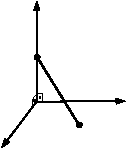
\includegraphics{part_1/chapter_3/figures/Figure2.pdf}};
		\node[right] (1) at (-0.4, 0.4) {$(0,0,1)$};
		\node[right] (2) at (0.4, -0.8) {$(1,1,0)$};	
	\end{tikzpicture}
    \caption{$(0,0,1)$ is degenerate if you add the constraint $x_2 \ge 0$} \label{p1c3:fig:redundancy_and_degeneration}
\end{figure}


\section{Optimality of extreme points}

Now that we have discussed how to algebraic represent extreme points and have seen a simple mechanism to iterate among their adjacent neighbours, the final element missing for us to be able to devise an optimisation method is to set the optimality conditions we wish to satisfy.


\subsection{The existence of extreme points}

First, let us define the condition that guarantee the existence of extreme points is a polyhedral set, otherwise, there is no hope hoping of finding an optimal solution.

\begin{definition}[Existence of extreme point]\label{p1c3:def:line_containing}
	A polyhedral set $P \subset \reals^n$ contains a line if $P \neq \emptyset$ and there exists a nonzero vector $d \in \reals^n$ such that $x + \lambda d \in P$ for all $\lambda \in \reals$.
\end{definition}

Figure \ref{p1c3:fig:line_containing} illustrates the notion of containing a line a the existence of extreme points. Notice that if a set would have any sort of ``kink'', then that would imply that a line is contained between the edges that form that kink, and that kink would be an extreme point.

\begin{figure}
	\begin{tikzpicture}
		\node at (0,0) {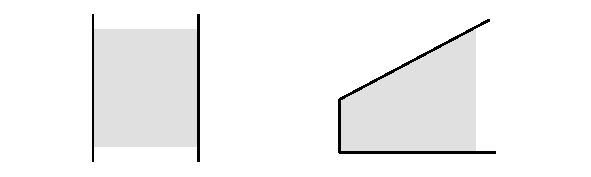
\includegraphics{part_1/chapter_3/figures/Figure3.pdf}};
		\node at (-2.5,0) {$P$};
		\node at (2,-0.3) {$Q$};		
	\end{tikzpicture}
	\caption{$P$ contains a line (left) and $Q$ does not contain a line (right)} \label{p1c3:fig:line_containing}	
\end{figure}

We are now ready to pose the result that utilises Definition \ref{p1c3:def:line_containing} to provide the conditions for the existence of extreme points.

\begin{theorem}[Existence of extreme points]\label{p1c3:thm:exist_extreme_point}
	Let $P = \braces{x \in \reals^n \mid a_i^\top x \geq b_i, i = 1, \dots, m} \neq \emptyset$ be a polyhedral set. Then the following are equivalent:
	\begin{enumerate}
		\item $P$ has at least one extreme point;
		\item $P$ does not contain a line;
		\item There exists $n$ LI vectors within $\braces{a_i}_{i=1}^m$.	
	\end{enumerate}	
\end{theorem}	 

% TODO: add a proof.

It tuns out that linear programming problems in the standard form do not contain a line, meaning that they will always provide at least one extreme point (or a basic feasible solution). More generally, bounded polyhedral sets do not contain a line, neither the positive orthant contain a line.

We are now to state the result that proves the intuition we had when analysing the plots in Chapter \ref{chapter_1}, which states that if a polyhedral set has at least one extreme point and at least one optimal solution, then there must be an optimal solution that is an extreme point.

\begin{theorem}[Optimality of extreme points]\label{p1c3:thm:opt_extreme}
		Let $P = \braces{x \in \reals^n \mid Ax \geq b}$ be a polyhedral set and $c \in \reals^n$. Consider the problem 
			\begin{equation*}
		    		z = \mini\braces{c^\top x : x \in P}.					
			\end{equation*}
		Suppose that $P$ has at least one extreme point and that there exists an optimal solution. Then, there exists an optimal solution that is an extreme point of $P$.
\end{theorem}

\begin{proof}
	Let $Q = \braces{x \in \reals^n \mid Ax \geq b, c^\top x = z}$ be the (nonempty) polyhedral set of all optimal solutions. Since $Q \subset P$ and $P$ contains no line (cf. Theorem \ref{p1c3:thm:exist_extreme_point}), $Q$ contains no line either, and thus has an extreme point.

	Let $\overline{x}$ be an extreme point of $Q$. By contradiction, assume that $\overline{x}$ is not an extreme point of $P$. Then, there exist $y \neq \overline{x}$, $z \neq \overline{x}$, and $\lambda \in [0,1]$ such that $\overline{x} = \lambda y + (1-\lambda)z$. Then, $c^\top \overline{x} = \lambda c^\top y + (1-\lambda)c^\top z$. As $z$ is optimal, we have that $z \leq c^\top y$ and $z \leq c^\top z$,  and thus $z = c^\top y = c^\top z$. 
	
	Thus, $z \in Q$ and $y \in Q$, contradicting that $\overline{x}$ is an extreme point. Thus, $\overline{x}$ must be an extreme point and, since we established that $\overline{x} \in Q$, it is also optimal. 
\end{proof}

Theorem \ref{p1c3:thm:opt_extreme} is posed in a somewhat general way, which by be a source for confusion. First, recall that in the example in Chapter \ref{chapter_1}, we considered the possibility of the objective function level curve associated with the optimal value to be parallel to one of the edges of the feasible region, meaning that instead of a single optimal solution (a vertex), we would observe a line segment containing an infinite number of optimal solutions, of which exactly two would be extreme points. 

In a more general case (with $n > 2$) it might be so that a whole facet of optimal solution is obtained. That is precisely the polyhedral set of all optimal solutions $Q$ in the proof. Clearly, this polyhedral set will not contain a line and, therefore (cf. Theorem \ref{p1c3:thm:exist_extreme_point}), have at least one extreme point. 

This is important because we intend to design an algorithm that only inspect extreme points. This discussion guarantees that, even for the cases in which a whole set of optimal solution exists, some elements in that set will be extreme points anyway, and thus identifiable by our method.


\subsection{Finding optimal solutions}

We now focus on the issue of being able to find and recognise extreme points as optimal solutions. In generally, optimisation methods iterate the following steps:
%
\begin{enumerate}
	\item Start from an initial (often feasible) solution;
	\item Find a nearby solution with better value;
	\item If none are available, return the best known solution.	
\end{enumerate}
%
This very simple procedure happens to be the core idea of the majority of the optimisation methods known. We will concentrate how to identify directions of improvement and, as consequence of their absence, how to identify optimality.

Starting from a point $x \in P$, we would like to move in a direction $d$ that yields improvement. Definition \ref{p1c3:def:feasible_direction} provides a formalisation of this idea.

\begin{definition}[Feasible directions] \label{p1c3:def:feasible_direction}
	Let $x \in P$, where $P \subset \reals^n$ is a polyhedral set. A vector $d \in \reals^n$ is a feasible direction at $x$ if there exists $\theta > 0$ for which $x + \theta d \in P$.
\end{definition}

Figure \ref{p1c3:fig:feasible_directions} provides an illustration of the concept. Notice that at extreme points, the relevant feasible directions are those along the edges of the polyhedral set, since those are the directions that can lead other other extreme points.
  
\begin{figure}
	\begin{tikzpicture}
		\node (0,0) {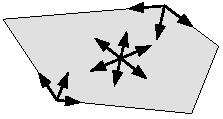
\includegraphics{part_1/chapter_3/figures/Figure4.pdf}};
		\node (P) at (-0.9,0.25) {$P$};
	\end{tikzpicture}
	\caption{Feasible directions at different points of $P$} \label{p1c3:fig:feasible_directions}
\end{figure}

Let us now devise a way of identifying feasible directions algebraically. for that, let $A$ be a $m \times n$ matrix, $I = \braces{1,\dots,m}$ and $J = \braces{1,\dots,n}$. Consider the problem 
%
\begin{equation*}
	\mini \braces{c^\top x : Ax = b, x \geq 0}.	
\end{equation*}
%
Let $x$ be a basic feasible solution (BFS) with basis basis $B = [A_{B(1)}, \dots, A_{B(m)}]$. Recall that the basic variables $x_B$ are given by
%
\begin{equation*}
	x_B = (x_{B(i)})_{i \in I_B} = B^{-1}b, \text{ with } I_B = \braces{B(1), \dots, B(m)} \subset J,	
\end{equation*}
%
and that the remaining variables, the nonbasic variables $x_N$ are such that $x_N = (x_j)_{j \in I_N} = 0$, with $I_N = J \setminus I_B$.

Moving to a neighbouring solution can be achieved by simply moving between adjacent basis, which can be accomplished  with very little computational burden. This entail first selecting a nonbasic variable $x_j$, $j \in I_N$, and increase it to a positive value $\theta$. 

Equivalently, we can define a \emph{feasible direction} $d = [d_N, d_B]$, $d_N$ represent the components associated with nonbasic variables and $d_B$ those associated with basic variables. The components associated with the nonbasic variables are thus simply defined as 
%
\begin{equation*}
d = \begin{cases} d_j = 1 \\ 
				  d_{j'} = 0, \text{for all } j' \neq j, 
	\end{cases}	
\end{equation*}
%
with $j, j' \in I_N$ and move from the point $x$ to the point $x + \theta d$. Notice that, geometrically, we are moving along a line in the dimension represented by the nonbasic variable $x_j$.

Now, feasibility might become an issue, if we are not careful to retain feasibility conditions. To retain feasibility, we must observe that $A(x + \theta d) = b$, implying that $Ad = 0$. This allows us to define the components of the direction vector $d$ that is associated with the basic variables $x_j$, $j \in I_B$, since
%
\begin{equation*}
	0 = Ad = \sum_{j = 1}^n	A_j d_j = \sum_{i = 1}^m A_{B(i)}d_{B(i)} + A_j = Bd_B + A_j
\end{equation*}
%
and thus $d_B = -B^{-1} A_j$ is the \emph{basic direction} implied by the choice of the nonbasic variable $x_j$, $j \in I_N$ to become basic. The vector $d_B$ can be though as the adjustments that must be made in the value of the other basic variables to accommodate the new variable becoming basic in order to retain feasibility. 

% TODO: this is a complicated concept using a complicated figure.  Rethink this showing a simple example (x_1 + x_2 + x_3 = 1, x_j >= 0) with the "normal feasible region" and the schematic 2d representation. by its side, showing that making 2 out of 3 variables nonbasic yields each of the corners of the triangle. 

Figure \ref{p1c3:fig:adjacent_vertices} provides a schematic representation of this process, showing how the change between adjacent basis can be seen as a movement between adjacent extreme points. Notice that it conveys a schematic representation of a $n=5$ dimensional problem, in which we ignore all the $m$ dimensions and concentrate on the $n-m$ dimensional projection of the feasibility set. This implies that the only constraints left are those associated with the nonnegativity of the variables $x \ge 0$, each associated with an edge of this alternative representation. Thus, when we set $n-m$ (nonbasic variables) to be zero, we identify an associated extreme point. As $n-m = 2$, we can plot this alternative representation.

\begin{figure}
	\begin{tikzpicture}
		\node (0,0) {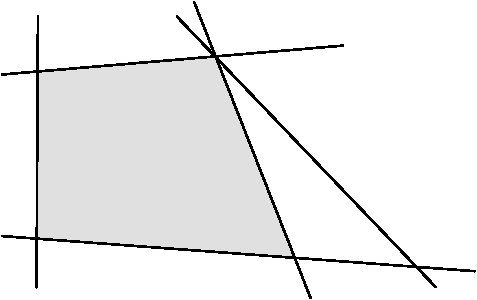
\includegraphics{part_1/chapter_3/figures/Figure5.pdf}};
		\node (A) at (-3.2, 1.65) {$A$};
		\node (B) at (-0.2, 1.9) {$B$};
		\node (C) at (3.1, -1.7) {$C$};
		\node[rotate = 90] (x1) at (-3.65, 0) {$x_1 = 0$};
		\node (x2) at (-1.2, -2) {$x_2 = 0$};
		\node (x3) at (-1.9, 1.75) {$x_3 = 0$};
		\node[left] (x4) at (0.25, 0) {$x_4 = 0$};
		\node[right] (x4) at (1.25, 0) {$x_5 = 0$};
	\end{tikzpicture}
	\caption{Example: $n = 5$ and $n-m = 2$. At $A$, $x_1 = x_3 = 0$ and $x_2, x_4, x_5 \geq 0$. Increasing $x_1$ while keeping $x_3$ zero leads to $B$. At $B$, suppose $I_N = \braces{3,5}$; by increasing $x_3$ while keeping $x_5$ zero would leads to $C$.} \label{p1c3:fig:adjacent_vertices}
\end{figure}

Clearly, overall feasibility, i.e., ensuring that $x \ge 0$ can only be retained if $theta > 0$ is chosen appropriately small. This can be achieve if the following is observed:
%
\begin{enumerate}
	\item All the other nonbasic variables remain valued at zero, that is, $x_{j'} = 0$ for $j' \in I_N \setminus \braces{j}$.	
	\item if $x$ is a \emph{nondegenerate} extreme point, then all $x_B > 0$ and thus $x_B + \theta d_B \geq 0$ for appropriately small $\theta > 0$. 
	\item if $x$ is a \emph{degenerate} extreme point: $d_{B(i)}$ might not be feasible since, for some $B(i)$, if $d_{B(i)} < 0$ and $x_{B(i)} = 0$, any $\theta > 0$ will make $x_{B(i)} < 0$.
\end{enumerate}
%
We will see later that we can devise a simply rule to define a value for $\theta$ that guarantees the above will be always observed. For now, we will put this discussion on hold, and focus on the issue on how to guide the choice of which nonbasic variable index $j \in I_N$ to select to become basic.


\subsection{Moving towards improved solutions}

A simple yet efficient way of deciding which nonbasic component $j \in I_N$ to make basic is to consider the immediate potential benefit that it would have for the objective function value. 

Specifically, if we move along the feasible direction $d$ as previously define, we have that the objective function value changes by 
%
\begin{equation*}
	c^\top d = c_B^\top d_B + c_j = c_j - c_BB^{-1}A_j,
\end{equation*}
%
where $c_B = (c_{B(1)}, \dots, c_{B(m)})$. The quantity $c_j - c_BB^{-1}A_j$ can be used, for example, in a greedy fashion, meaning that we choose the nonbasic variable index $j \in I_N$ with greatest \emph{potential of improvement}.

First, let us formaly define this quantity, which is know as the \emph{reduced cost}. 

\begin{definition}[Reduced cost]
	Let $x$ be a basic solution associated with the basis $B$ and objective value vector $c_B$. For each nonbasic variable $x_j$, with $j \in I_N$, we define the reduced cost $\overline{c}_j$ as
	%
	\begin{equation*}
		\overline{c}_j = c_j - c_B^\top B^{-1}A_j.
	\end{equation*}
\end{definition}

The name reduced cost is motivated by the fact that it quantifies a cost change onto the reduced space of the basic variables. In fact, the reduced cost is calculating the change in the objective function caused by the increase in one unit of the nonbasic variable $x_j$ elected to become basic (represented by the $c_j$ component) and the associated change caused by the accommodation in the basic variable values to retain feasibility, as discussed in the previous section. Therefore, the reduced cost can be understood as a \emph{marginal value} of change in the objective function value associated with each nonbasic variable.

Let us demonstrate the this with a numerical example. Consider the following linear programming problem
%
\begin{align*}
	\mini & c_1x_1 + c_2x_2 + c_3x_3 + c_4x_4 \\	
	\st & x_1 + x_2 + x_3 + x_4 = 2 \\
	& 2x_1 + 3x_3 + 4x_4 = 2 \\
	& x_1, x_2 ,x_3, x_4 \geq 0.  
\end{align*}  
%
Let $I_B = \braces{1,2}$, yielding
% 
\begin{equation*}
	B = \begin{bmatrix}
    		1 & 1 \\
    		2 & 0
    	\end{bmatrix}.
\end{equation*} 
%
Thus, $x_3= x_4 =0$ and $x = (1,1,0,0)$. The basic direction $d_B$ for $x_3$ is given by
%
\begin{equation*}
    d_B = -B^{-1}A_3 = -\begin{bmatrix}
    	0 & 1/2 \\
    	1 & -1/2
    \end{bmatrix} \begin{bmatrix}
    	1 \\ 3
    \end{bmatrix} = \begin{bmatrix}
    	-3/2 \\ 1/2
    \end{bmatrix}.
\end{equation*}
%
The ``cost'' of moving along this direction is 
%
\begin{equation*}
	c^\top d = -3c_1/2 + c_2/2 +c_3 = c_3 - (c_1, c_2)^\top d_B.
\end{equation*}

Clearly, the willingness for choosing $x_3$ as the variable to become basic will depend on whether the scalar $c_3 - (c_1, c_2)^\top d_B$ is negative (recall that we want to minimise the problem, so the smaller the total cost, the better). Another point is how large in module the reduced cost is. Recall that the reduced is in fact a measure of the marginal value associated with the increase in value of the nonbasic variable, and thus the higher (in module) it his, the quicker the objective function value will decrease per unit of increase of the nonbasic variable value.

One interesting thing to notice is what is the reduced cost associated with basic variables. Recall that $B = [A_{B(1)}, \dots, A_{B(m)}]$ and thus $B^{-1}[A_{B(1)}, \dots, A_{B(m)}] = I$. Therefore $B^{-1}A_{B(i)}$ is the $i^\text{th}$ column of $I$, denoted $e_i$, implying that
%
\begin{equation*}
	\overline{c}_{B(i)} = c_{B(i)} - c^\top_B B^{-1} A_{B(i)} = c_{B(i)} - c_B^\top e_i = c_{B(i)} - c_{B(i)} = 0.	
\end{equation*}


\subsection{Optimality conditions}

Now that we have seen how to identify promising directions for improvement, we have incidentally developed a framework to identifying optimality of a given basic feasible solution (BFS). That is, a BFS that from which no direction of improvement can be observed must be locally optimal. And, since local optimality implies global optimality in the presence of convexity (the convexity of linear programming problems was attested in Chapter \ref{chapter_2}; the global optimality in the presence of convexity is a results discussed in detail in \ref{part_2}), we can declare this BFS as an optimal solution. 

Theorem \ref{p1c3:thm:opt_conditions} establishes the optimality of a BFS from which no improving feasible direction can be found without relying on the notion of convexity.

\begin{theorem}[Optimality conditions]\label{p1c3:thm:opt_conditions}
	Consider the problem $P : \mini\braces{c^\top x : Ax = b, x \geq 0}$. Let $x$ be the BFS associated with a basis $B$ and let $\overline{c}$ be the corresponding vector of reduced costs.
	\begin{enumerate}
		\item if $\overline{c} \geq 0$, then $x$ is optimal.
		\item if $x$ is optimal and nondegenerate, then $\overline{c} \geq 0$.	
	\end{enumerate}
\end{theorem}

\begin{proof}
To prove (1), assume that $\overline{c}_j \geq 0$, let $y$ be a feasible solution to $P$, and $d = y - x$. We have that $Ax = Ay = b$ and thus $Ad = 0$. Equivalently:
%
\begin{align}
	&B d_B + \sum_{j \in I_N}A_j d_j = 0 \Rightarrow d_B = - \sum_{j \in I_N}B^{-1}A_jd_j, \text{ implying that } \nonumber \\
	&c^\top d = c_B^\top d_B + \sum_{j \in I_N}c_jd_j= \sum_{j \in I_N} (c_j - c_B^\top B^{-1}A_j)d_j = \sum_{j \in I_N}\overline{c}_jd_j \label{p1c3:eq:red_cost_opt_cond}
\end{align}
%
We have that $x_j = 0$ and $y_j \geq 0$	for $j \in I_N$. Thus, $d_j \geq 0$ and $\overline{c}_jd_j \geq 0$ for $j \in I_N$, which implies that $c^\top d \geq 0$ (cf. \eqref{p1c3:eq:red_cost_opt_cond}). Consequently,
%
\begin{equation*}
	c^\top d \geq 0 \Rightarrow	c^\top (y - x) \geq 0 \Rightarrow c^\top y \geq c^\top x, \text{ i.e., $x$ is optimal.}
\end{equation*}
%
To prove (2) by contradiction, assume that $x$ is optimal with $\overline{c}_j < 0$ for some $j \in I_N$. Thus, we could improve on $x$ moving along this $j^\text{th}$ direction $d$, contradicting the optimality of $x$.
\end{proof}

A couple of remarks are worth making at this point. First, notice that, in the presence of degeneracy, it might be that $x$ is optimal with $\overline{c}_j < 0$ for some $j \in I_N$. Luckily, the simplex method manages to get around this issue in an effective manner, as we will see in the next chapter. Another point to notice is that, if $\overline{c}_j > 0$, $\forall j \in I_N$ then $x$ is a \emph{unique optimal}. Analogously, if $\overline{c} \geq 0$ with $c_j =0$ for some $j \in I_N$, then it means that moving in that direction will cause no change in the objective function value, implying that both BFS are ``equally optimal'' and that the problem has multiple optimal solutions. 





	 
		
	
	\part{Nonlinear optimisation} \label{part_2}
		
	\chapter{Introduction}
	\section{What is optimisation?}

An optimisation is one of these words that has many meanings, depending on the context you take as a reference. In the context of this course, optimisation refers to \emph{mathematical optimisation}, which is a discipline of applied mathematics.

In mathematical optimisation, we build upon concepts and techniques from calculus, analysis, linear algebra, and other domains of mathematics to develop methods that allow us finding values for variables within a given domain that maximise (or minimise) the value of a function. In specific, we are trying to solve the following general problem:
%
\begin{align}
    \min &f(x) \label{eq:opt_prob} \\
    \text{s.t.}   &x \in X. \nonumber
\end{align}
%
%where $x \in \reals^n$ is a vector of $n$ \emph{variables}, $f:\mathbb{R}^n \mapsto \reals$ is a \emph{function} to be optimised (minimised) and $X \subseteq \reals^n$ is a \emph{domain} containing acceptable values for $x$.

In a general sense, these problems can be solved by employing the following strategy:
%
\begin{enumerate}
    \item Analysing properties of functions under specific domains and deriving the conditions that must be satisfied such that a point $x$ is a candidate optimal point.
    \item Applying numerical methods that iteratively searches for points satisfying these conditions. 
\end{enumerate}
%
This idea is central in several domains of knowledge, and very often are defined under area-specific nomenclature. Fields such as economics, engineering, statistics, machine learning and, perhaps more broadly, operations research, are intensive users and developers of optimisation theory and applications. 

\subsection{Mathematical programming and optimisation}

Operations research and mathematical optimisation are somewhat intertwined, as they both were born around a similar circumstance. %(Include something on the history of OR)

I like to separate \emph{mathematical programming} from (mathematical) \emph{optimisation}. Mathematical programming is a modelling paradigm, in which we rely on (very powerful, I might add) analogies to model \emph{real-world} problems. In that, we look at a given decision problem considering that
%
\begin{itemize}
    \item \emph{variables} represent \emph{decisions}, as in a business decision or a course of action. Examples include setting the parameter of (e.g., prediction) model, production systems layouts, geometries of structures, topologies of networks, and so forth; 
    \item \emph{domain} represents business rules or \emph{constraints}, representing logic relations, design or engineering limitations, requirements, and such; 
    \item function is an \emph{objective function} that provides a measure of solution quality.  
\end{itemize}
%    
With these in mind, we can represent the decision problem as a \emph{mathematical programming model} of the form of \eqref{eq:opt_prob} that can be solved using \emph{optimisation} methods. From now on, we will refer to this specific class of models as mathematical optimisation models, or optimisation models for short. We will also use the term to \emph{solve the problem} to refer to the task of finding optimal solutions to optimisation models.

This course is mostly focused on the optimisation techniques employed to find optimal solutions for these models. As we will see, depending on the nature of the functions $f$ and $g$ that are used to formulate the model, some methods might be more or less appropriate. Further complicating the issue, for models of a given nature, there might be alternative algorithms that can be employed and with no generalised consense whether one method is generally better performing than another.

\subsection{Types of mathematical optimisation models}

In general, the simpler the assumptions on the parts forming the optimisation model, the more efficient are the methods to solve such problems. 

Let us define some additional notation that we will use from now on. Consider a model in the general form
%
\begin{align*}
	\mini & f(x) \\
	\st   & g_i(x) \leq 0, i = 1, \dots, m \\
	      & h_i(x) = 0, i = 1, \dots, l \\
	      & x \in X,  
\end{align*}
%
where $f: \reals^n \mapsto \reals$ is the objective function, $g:\reals^m \mapsto \reals^m$ is a collection of $m$ inequality constraints and $h: \reals^n \mapsto \reals^l$ is a collection of $l$ equality constraints.

{\bf Remark:} in fact, every inequality constraint can be represented by an equality constraint by making $h_i(x) = g_i(x) + x_{n+1}$ and augmenting the decision variable vector $x \in \reals^n$ to include the slack variable $x_{n+1}$. However, since these constraints are of very different nature, we will explicitly represent both whenever necessary.

The most general types of models are the following. We also use this as an opportunity to define some (admittedly confusing) nomenclature from the field of operations research that we will be using in these notes.
%
\begin{enumerate}
    \item \emph{Unconstrained models:} in these, the set $X = \reals^n$ and $m=l=0$. These are prominent in, e.g., machine learning and statistics applications, where $f$ represents a measure of model fitness or prediction error.  
    \item \emph{Linear programming (LP):} presumes linear objective function. $f(x) = c^\top x$ and constraints $g$ and $h$ affine, i.e., of the form $a_i^\top x - b_i$, with $a_i \in \reals^n$ and $b \in \reals$. Normally, $X = \braces{x \in \reals^n \mid x_j \geq 0, j = 1,\dots, n}$ enforce that decision variables are constrained to be the nonnegative orthant.
    \item \emph{Nonlinear programming (NLP):} some or all of the functions $f$, $g$, and $h$ are nonlinear.
    \item \emph{Mixed-integer (linear) programming (MIP):} consists of an LP in which some (or all) of the variables are constrained to be integers. In other words, $X \subseteq \reals^k \times \integers^{n-k}$. Very frequently, the integer variables are binary terms, i.e., $x_i \in \braces {0,1}$, for $i = 1,\dots, n-k$ and are meant to represent true-or-false or yes-or-no conditions.
    \item \emph{Mixed-integer nonlinear programming (MINLP):} are the intersection of MIPs and NLPs.  
\end{enumerate}

{\bf Remark:} notice that we use the vector notation $c^\top x = \sum_{j \in J} c_j x_j$, with $J = \braces{1,\dots,N}$. This is just a convenience for keeping the notation compact. 


\section{Examples of applications}


We now discuss a few examples to illustrate the nature of the problems to which we will develop solution methods and their applicability to real-world contexts. 

\subsection{Resource allocation and portfolio optimisation} \label{sec:resource_allocation}

In a general sense, any mathematical optimisation model is an instantiation of the \emph{resource allocation problem}. A resource allocation problem consists of how to design an optimal allocation of resources to tasks, such that a given outcome is optimised. 

Classical examples typically include production planning settings, in which raw materials or labour resources are inputted into a system and a collection of products, a production plan, results from this allocation. The objective is to find the best production plan, that is, a plan with the maximum profit or minimum cost. Resource allocation problems can also appear in a less obvious setting, where the resources can be the capacity of transmission lines in an energy generation planning setting, for example.

Let $i \in I = \braces{1,\dots, M}$ be a collection of resources and $j \in J = \braces{1,\dots,N}$ be a collection of products. Suppose that, to produce one unit of product $j$, a quantity $a_{ij}$ of resource $i$ is required. Assume that the total availability of resource $i$ is $b_i$ and that the return per unit of product $j$ is $c_j$.

Let $x_j$ be the decision variable representing total of product $j$ produced. The resource allocation problem can be modelled as
%
\begin{align}
	\maxi \ & \sum_{j \in J} c_j x_j \label{ex1:obj} \\
	\st & \sum_{j \in J}a_{ij} x_j \leq b_i, \ \forall i \in I \label{ex1:const1} \\
	& x_j \geq 0, \ \forall j \in J. \label{ex1:const2}
\end{align} 
%
Equation \eqref{ex1:obj} represents the objective function, in which we maximise the total return obtained from a given production plan. Equation \eqref{ex1:const1} quantify the resource requirements for a given production plan and enforce that such a requirement does not exceed the resource availability. Finally, constraint \eqref{ex1:const2} defines the domain of the decision variables.

Notice that, as posed, the resource allocation problem is linear. This is perhaps the most basic, and also most diffused setting for optimisation models for which very reliable and mature technology is available. In this course, we will concentrate on methods that can solve variants of this model in which the objective function and/or the constraints are required to include nonlinear terms. 

One classic variant of resource allocation that include nonlinear terms is the \emph{portfolio optimisation problem}. In this, we assume that a collection of assets $j \in J = \braces{1,\dots, N}$ are available for investment. In this case, capital is the single (actual) resource to be considered. Each asset has random return $R_j$, with an expected value $\mathbb{E}[R_j] = \mu_j$. Also, the covariance between two assets $i,j \in J$ is given by $\sigma_{ij} = \mathbb{E}[(R_i - \mu_i)(R_j - \mu_j)]$, which can be denoted as the covariance matrix 
%
\begin{align*}
	\Sigma = \begin{bmatrix}
		\sigma_{11} & \dots & \sigma_{1N} \\ 
		\vdots      & \ddots & \vdots \\
		\sigma_{N1}  & \dots & \sigma_{NN}
	\end{bmatrix}
\end{align*}
%
Markowitz (1952) proposed using $x^\top\Sigma x$ as a risk measure that captures the variability in the return of the assets. Given the above, the optimisation model that provides the investment portfolio with the least risk, given a minimum requirement $\epsilon$ in terms of expected returns is given by
%
\begin{align}
	\mini \ &  x^\top\Sigma x \label{ex2:obj} \\
	\st & \mu^\top x  \geq \epsilon \label{ex2:const1}\\
	& 0 \leq x_j \leq 1, \ \forall j \in J. \label{ex2:const2}
\end{align} 
%
Objective function \eqref{ex2:obj} represents the portfolio risk to be minimised, while constraint \eqref{ex2:const1} enforces that the expected return must be at least $\epsilon$. Notice that $\epsilon$ can be seen as a resource that has to be (at least) completely depleted, if one wants to do a parallel with the resource allocation structure discussed early. Constraint \eqref{ex2:const2} defined the domain of the decision variables. Notice how the problem is posed in a scaled form, where $x_j \in [0,1]$ represents a percentage of a hypothetical available capital for investment.

In this example, the problem is nonlinear due to the quadratic nature of the objective function $x^\top\Sigma x = \sum_{i,j \in J} \sigma_{ij}x_ix_j$. As we will see later on, there are efficient methods that can be employed to solve quadratic problems like this.


\subsection{The pooling problem: refinery operations planning}

The \emph{pooling problem} is another example of a resource allocation problem that naturally presents nonlinear constraints. In this case, the production depends on \emph{mixing operations}, known as pooling, to obtain certain product specification for a given property.

As an illustration, suppose that products $j \in J = \braces{1,\dots,N}$ are produced by mixing byproducts $i \in I_j \subseteq I = \braces{1,\dots,M}$. Assume that the qualities of byproducts $q_i$ are known and that there is no reaction between byproducts. Each product is required to have a property value $q_j$ within an acceptable range $[\underline{q}_j, \overline{q}_j]$ to be classified as product $j$. In this case, mass and property balances are calculated as
%
\begin{align}
	& x_j  = \sum_{i \in I_j}{x_i}, \ \forall j \in J \\
	& q_j = \frac{\sum_{i \in I_j}q_ix_i}{x_j}, \ \forall j \in J \label{ex3:const2}.
\end{align}
%
These can then incorporated into the resource allocation problem accordingly. One key aspect associated with pooling problem formulations is that the property balances represented by \eqref{ex3:const2} define \emph{nonconvex} feasibility regions. As we will see later, convexity is a powerful property that allows for developing efficient solution methods and its absence typically compromises computational performance and tractability in general.

  
\subsection{Robust optimisation}

Robust optimisation is a subarea of mathematical programming concerned with models that support decision-making under \emph{uncertainty}. In specific, the idea is to devise a formulation mechanism that can guarantee feasibility of the optimal solution in face of variability, ultimately taking a risk-averse standpoint. 

Consider the resource allocation problem from Section \ref{sec:resource_allocation}. Now, suppose that the parameters $\tilde{a}_i \in \reals^N $ associated with a given constraint $i \in I = \braces{1,\dots,M}$ are uncertain with a unknown probability distribution. The resource allocation problem can then be formulated as
%
\begin{align*}
	\maxi \ &  c^\top x  \\
	\st & \tilde{a}_{i}^\top x \leq b_i, \ \forall i \in I  \\
	& x_j \geq 0, \ \forall j \in J. 
\end{align*} 
%
Let us assume that the only information available are observations $\hat{a}_i$, from which we can estimate a nominal value $\overline{a}_i$. This is illustrated in Figure \ref{fig:random_observations}, in which 100 random observations are generated for $\tilde{a_i} = [\tilde{a}_{i1}, \tilde{a}_{i2}]$ with $\tilde{a}_{i1} \sim \text{Normal}(10,2)$ and $\tilde{a}_{i2} \sim \text{Normal}(5,3)$ for a single constraint $i \in I$. The nominal values are assumed to have coordinates given by the average values used in the Normal distributions. 
%
\begin{figure}[h]
	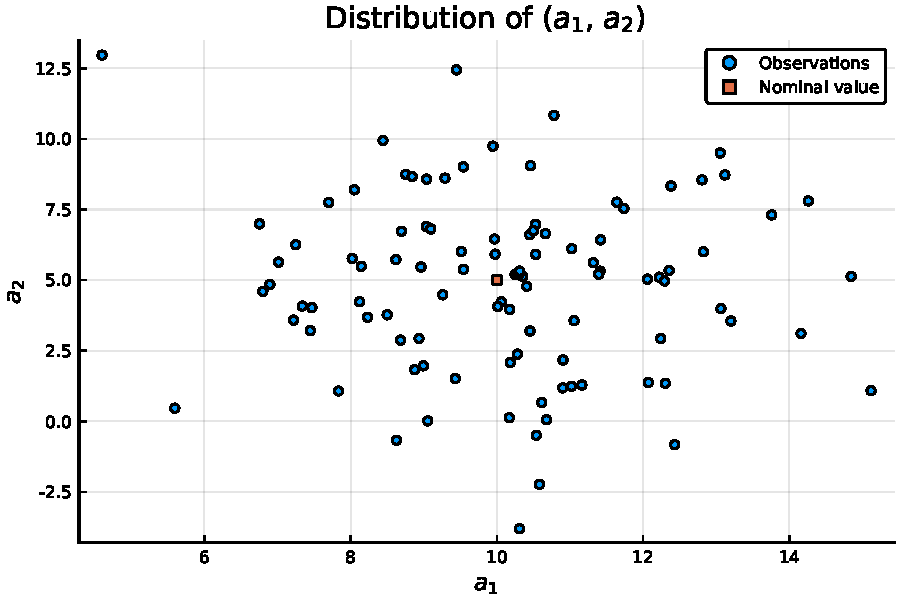
\includegraphics[width=0.8\textwidth]{part_2/chapter_1/figures/data_no_ellipsoid.pdf}
	\caption{One hundred random realisations for $\tilde{a}_i$.} \label{fig:random_observations}
\end{figure}
%
Our objective is to develop a model that incorporates a given level of protection in terms of feasibility guarantees. That is, we would like to develop a model that provides solutions that are guaranteed to remain feasible if the realisation of $\tilde{a}_i$ falls within an \emph{uncertainty set} $\epsilon_i$ of size controlled by the parameter $\Gamma_i$. The idea is that the bigger the uncertainty set $\epsilon_i$, the more robust is the solution, which typically comes at the expense of accepting solutions with expected worse performance.

The tractability of robust optimisation models depends on the geometry of the uncertainty set employed. Let us assume in what follows that 
%
\begin{align}
	\epsilon_i = \braces{\overline{a}_i + P_iu \mid ||u||_2 \leq \Gamma_i} \label{eq:ellipsoid}
\end{align}
%
is an ellipsoid with the characteristic matrix $P_i$ (i.e., its eigenvalues show how the ellipsoid extends in every direction from $\overline{a}_i$) and $\Gamma_i$ employs a scaling of the ellipsoid size.

{\bf Remark:} an alternative (perhaps more frequent) characterisation of an ellipsoid $\epsilon \subset \reals^n$ centred at $\overline{x}$ is given by $\epsilon = \braces{x \in \reals^n \mid (x - \overline{x})^\top A(x - \overline{x}) = 1}$. By making $A = P^{-2}$, we recover the representation in \eqref{eq:ellipsoid}.

We can now formulate the \emph{robust counterpart}, which consists of a risk-averse version of the original resource allocation problem. In that, we try to anticipate the worst possible outcome and make decisions that are both optimal and guarantee feasibility in this worst-case sense. This standpoint translates into the following optimisation model.
%
\begin{align}
	\maxi \ &  c^\top x \nonumber \\
	\st & \maxi_{a_{i} \in \epsilon_i}\braces{a_i^\top x} \leq b_i, \ \forall i \in I \label{ex3:robust_const}\\
	& x_j \geq 0, \forall j \in J. \nonumber
\end{align}
%
Notice how the constraint \eqref{ex3:robust_const} has an embedded optimisation problem, turning into a \emph{bi-level optimisation} problem. This highlights the issue associated with tractability, since solving the whole problem strongly depends on deriving tractable equivalent reformulations.

Assuming that the uncertainty set $\epsilon_i$ is an ellipsoid, the following result holds.
%
\begin{align}
	\max_{a_{i} \in \epsilon_i}\braces{a_i^\top x}  & = \overline{a}_i^\top x + \max_u\braces{u^\top P_i x : ||u||_2 \leq \Gamma_i} \label{eq:robust_set1}\\
	& = \overline{a}_i^\top x + \Gamma_i||P_i x||_2. \label{eq:robust_set2}
\end{align}
%
In \eqref{eq:robust_set1}, we recast the inner problem in terms of the ellipsoidal uncertainty set, ultimately meaning that we recast the inner maximisation problem in terms of variable $u$. Since the only constraint is $||u||_2 \leq \Gamma_i$, in \eqref{eq:robust_set2} we can derive a closed form for the inner optimisation problem.

With the closed form derived in \eqref{eq:robust_set2}, we can reformulate the original bi-level problem as a tractable single-level problem of the following form
%
\begin{align}
	\maxi \ &  c^\top x \nonumber \\
	\st & \overline{a}_i^\top x + \Gamma_i||P_i x||_2 \leq b_i, \ \forall i \in I \label{eq:robust_counter1}\\
	& x_j \geq 0, \ \forall j \in J. \nonumber
\end{align} 
%
Notice how the term $\Gamma_i||P_i^\top x||_2$ creates a buffer for constraint \eqref{eq:robust_counter1}, ultimately preventing the complete depletion of the resource. Clearly, this will lead to a suboptimal solution when compared to the original deterministic at the expense of providing protection against deviations in coefficients $a_i$. This difference is often referred to as the \emph{price of robustness}.

In Figure \ref{fig:ellipsoids}, we show the ellipsoidal sets for two levels of $\Gamma_i$ for a single constraint $i$. We define 
%
\begin{align}
	\epsilon_i = \braces{\begin{bmatrix} 10 \\ 5 \end{bmatrix} + \begin{bmatrix} 2 & 0 \\ 0 & 3 \end{bmatrix} \begin{bmatrix} u_1 \\ u_2 \end{bmatrix}}
\end{align}
%
using the average and standard deviation of the original distributions that generated the observations. We plot the ellipsoids for $\Gamma_1 = 1$ and $\Gamma_2 = 1.5$, illustrating how the protection level increases as $\Gamma$ increases. This can be inferred since the uncertainty set covers more of the observations and the formulation is such that feasibility is guaranteed for any observation within the uncertainty set. 
%
\begin{figure}
	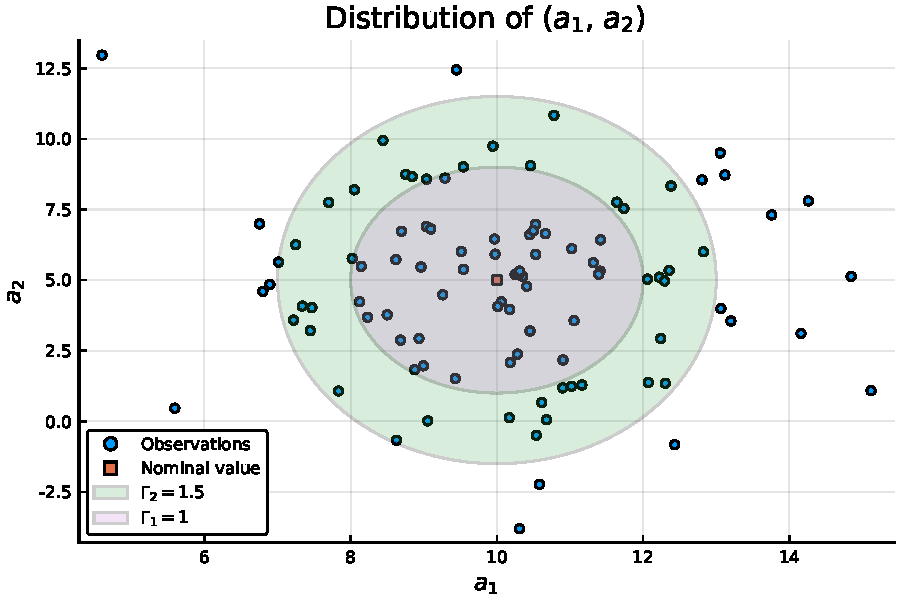
\includegraphics[width=0.8\textwidth]{part_2/chapter_1/figures/data_with_ellipsoid.pdf}
	\caption{One hundred random realisations for $\tilde{a}_i$.} \label{fig:ellipsoids}
\end{figure}
%


\subsection{Classification: support-vector machines}

This is an example in which the resource allocation structure within the optimisation model is not as obvious. Suppose we are given a data set $D \in \reals^{n}$ with $|D| = N + M$ that can be divided into two disjunct sets $I^- = \braces{x_1, \dots, x_N}$ and $I^+ = \braces{x_1,\dots, x_M}$. 

Each element in $D$ is an observation of a given set of $n$ features with values represented by a $x \in \reals^n$ that has been classified as belonging to set $I^-$ and $I^+$. Because of the availability of labelled data, classification is said to be ane xample of supervised learning in the field of machine learning. 

Figure \ref{fig:classified_observations} illustrates this situation for $n = 2$, in which the orange dots represent points classified as belonging to $I^-$ (negative observations) and the blue dots represent points classified as belonging to $I^+$ (positive observations).

\begin{figure}
    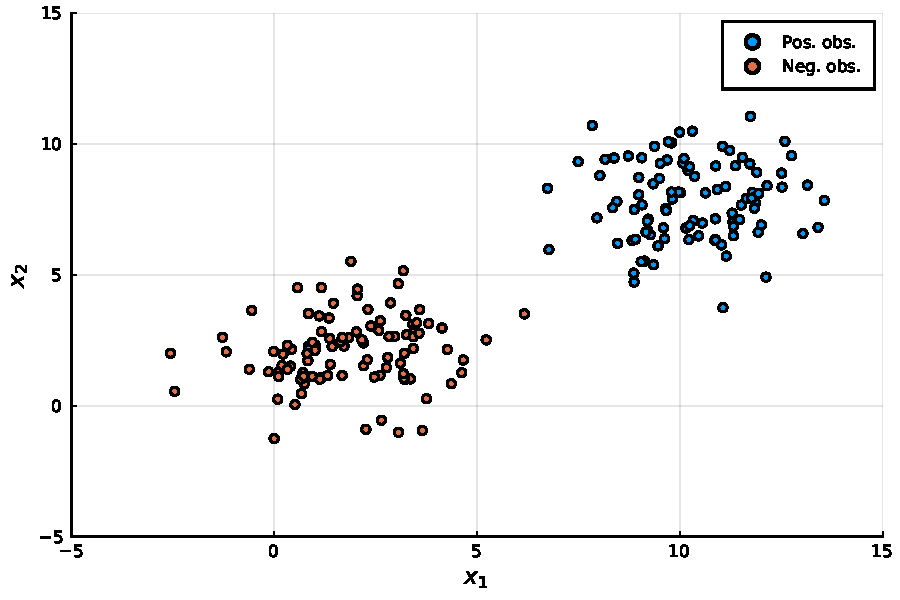
\includegraphics[width=0.8\textwidth]{part_2/chapter_1/figures/classes_no_classifier.pdf}
    \caption{Two hundred observations for $x_i$ classified to belong to $I^-$ (orange) or $I^+$ (blue).}        
    \label{fig:classified_observations}
\end{figure}

Our task is to obtain a function $f:\reals^n \mapsto \reals$ from a given family of functions that is capable to, given an observed set of features $\hat{x}$, classify whether it belongs to $I^-$ or $I^+$. In other words, we want to calibrate $f$ such that
%
\begin{align}
	f(x_i) < 0, \ \forall x_i \in I^-, \text{ and } f(x_i) > 0, \ \forall x_i \in I^+.  
\end{align}
%
This function would then act as a classifier that could be employed to any new observation $\hat{x}$ made. If $f$ is presumed to be an affine function of the form $f(x) = a^\top x - b$, then we obtain a \emph{linear classifier}. 

Our objective is to obtain $a \in \reals^n$ and $b \in \reals$ such that misclassification error is minimised. Let us define the error measure as
%
\begin{align*}
& e^-(x_i \in I^-; a, b) := 
    \begin{cases} 0, \text{ if } a^\top x_i - b \leq 0, \\
        a^\top x_i - b, \text{ if } a^\top x_i - b > 0.
    \end{cases} \\
& e^+(x_i \in I^+; a, b) := 
    \begin{cases} 0, \text{ if } a^\top x_i - b \geq 0, \\
        b -  a^\top x_i, \text{ if } a^\top x_i - b < 0.
    \end{cases}                   
\end{align*}
%
Using this error measure, we can define constraints that capture deviation on each measure by means of nonnegative slack variables. Let $u_i \geq 0$ for $i = 1, \dots, N$ and $v_i \geq 0$ for $i = 1,\dots, M$ be slack variables that measure the \emph{misclassification error} for $x_i \in I^-$ and $x_i \in I^+$, respectively.

The optimisation problem that finds optimal parameters $a$ and $b$ can be stated as
%
\begin{align}
	\mini \ & \sum_{i=1}^M u_i + \sum_{i=1}^N v_i \label{ex4:obj}\\
	\st & a^\top x_i - b - u_i \leq 0, i = 1, \dots, M \label{ex4:const1} \\
    & a^\top x_i - b + v_i \geq 0, i = 1,\dots,N \label{ex4:const2} \\
    & ||a||_2 = 1 \label{ex4:const3} \\
    & u_i \geq 0, i = 1, \dots, N \\
    & v_i \geq 0, i = 1, \dots, M \\
    & a \in \reals^n, b \in \reals. \label{ex4:end}   
\end{align} 
%
The objective function \eqref{ex4:obj} accumulates the total misclassification error. Constraint \eqref{ex4:const1} allows for capturing the misclassification error for each $x_i \in I^-$. Notice that $u_i = \max\braces{0, a^\top x_i -b} = e^-(x_i \in I^-; a, b)$. Likewise, constraint \eqref{ex4:const2} guarantees that $v_i = e^+(x_i \in I^+; a, b)$.
To avoid trivial solutions in which $(a,b) = (0, 0)$, the normalisation constraint $|| a ||_2 = 1$ is imposed in constraint \eqref{ex4:const3}, which turns the model nonlinear.

Solving the model \eqref{ex4:obj}--\eqref{ex4:end} provides optimal $(a,b)$ which translates into the classifier represented as the green line in Figure \ref{fig:observations_with_classifier}.

\begin{figure}[h]
    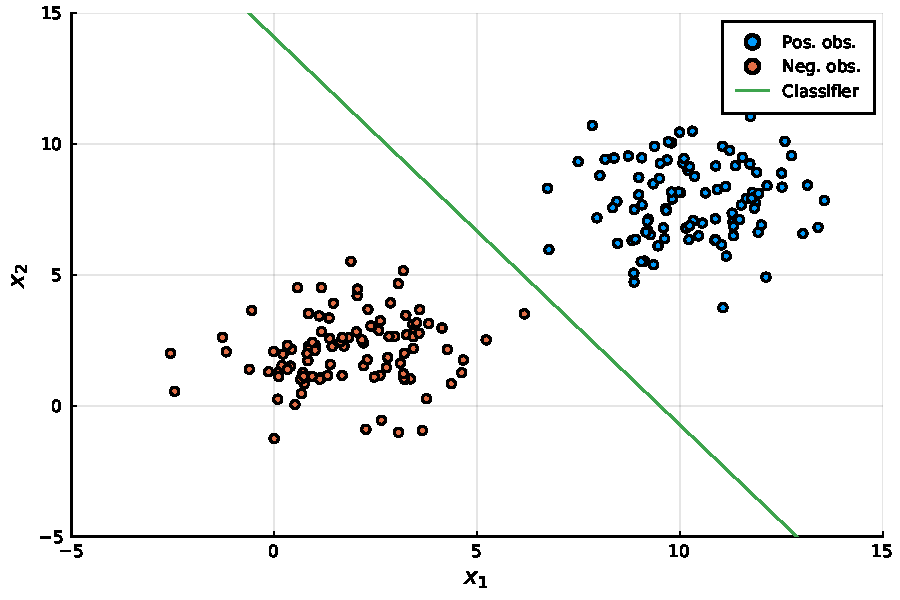
\includegraphics[width=0.8\textwidth]{part_2/chapter_1/figures/classes_with_classifier.pdf}
    \caption{Two hundred observations for $x_i$ classified to belong to $I^-$ (orange) or $I^+$ (blue) with a classifier (green).}        
    \label{fig:observations_with_classifier}
\end{figure}
 
A variant referred to as \emph{robust classifier} penalises not only the the misclassification error, but also the observations within a given slab $S = \braces{x \in \reals^n \mid -1 \leq a^\top x - b \leq 1}$. Notice that, being the two lines defined by $f^-(x) : a^\top x - b = -1$ and $f^+(x) : a^\top x - b = +1$, the distance between the two hyperplanes is given by $\frac{2}{||a||_2}$. 

Accordingly, we redefine our error measures as follows. 
%
\begin{align*}
	& e^-(x_i \in I^-; a, b) := 
	    \begin{cases} 0, \text{ if } a^\top x_i - b \leq -1, \\
	        |a^\top x_i - b|, \text{ if } a^\top x_i - b > -1.
	    \end{cases} \\
	& e^+(x_i \in I^+; a, b) := 
	    \begin{cases} 0, \text{ if } a^\top x_i - b \geq 1, \\
	        |b -  a^\top x_i|, \text{ if } a^\top x_i - b < 1.
	    \end{cases}                   
\end{align*}
%
By doing so, a penalty is applied not only to those points that were misclassified but also to those points correctly classified that happen to be inside the slab $S$. To define an optimal robust classifier, one must trade off the size of the slab, which is inversely proportional to $||a||$, and the total of observations that fall in the slab $S$. The formulation for the robust classifier then becomes
%
\begin{align}
	\mini \ & \sum_{i=1}^M u_i + \sum_{i=1}^N v_i + \gamma||a||_2^2 \label{ex5:obj}\\
	\st & a^\top x_i - b - u_i \leq -1, \ i = 1,\dots,M \label{ex5:const1} \\
	    & a^\top x_i - b + v_i \geq 1, \ i = 1,\dots,N \label{ex5:const2} \\
	    & u_i \geq 0, i = 1, \dots, N \\
	    & v_i \geq 0, i = 1, \dots, M \\
	    & a \in \reals^n, b \in \reals.
\end{align} 
%  
In objective function \eqref{ex5:obj}, the errors accumulated in variables $u_i$, $i=1,\dots,N$ and $v_i$, $i = 1,\dots,M$ and the squared norm $||a||_2^2$ are considered simultaneously. The term $\gamma$ is a scalar used to impose an emphasis on minimising the norm $||a||_2$ and incentivising a larger slab $S$ (recall that the slab is large for smaller $||a||_2$). The squared norm  $||a||_2^2$ is considered instead as a means to recover differentiability, as the norm  $||a||_2$ is not differentiable. Later on, we will see how beneficial it is for optimisation methods to be able to assume differentiability. Moreover, note how in constraints \eqref{ex5:const1} and \eqref{ex5:const2} $u$ and $v$ also accumulate penalties for correctly classified $x_i$ that happen to be between the slab $S$, that is, that have term $a^\top x - b$ larger/ smaller than -1/ +1. Figure \ref{fig:observations_with_rob_classifier} shows a robust classifier an arbitrary value of $\gamma$.

\begin{figure}[H]
    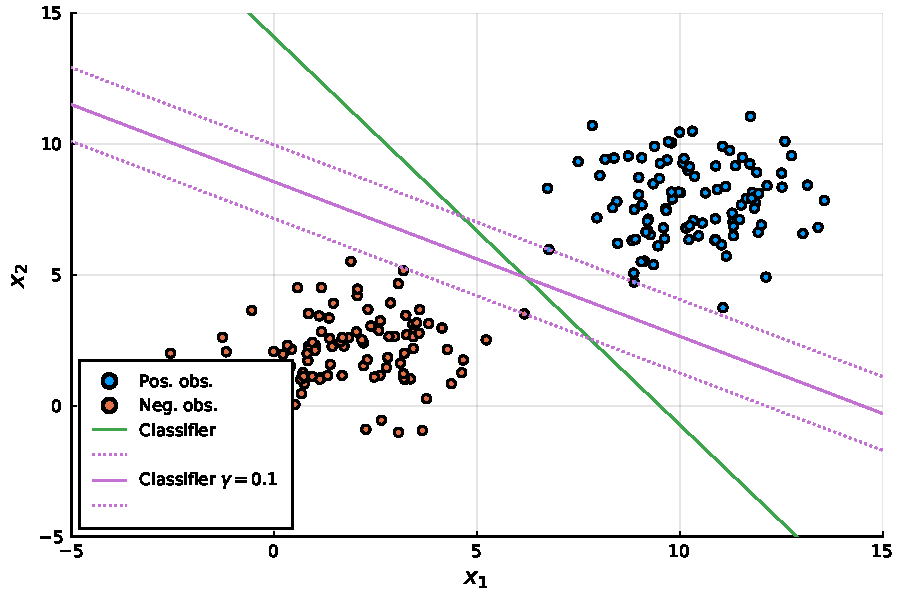
\includegraphics[width=0.8\textwidth]{part_2/chapter_1/figures/classes_with_robust_classifier.pdf}
    \caption{Two hundred observations for $x_i$ classified to belong to $I^-$ (orange) or $I^+$ (blue).}        
    \label{fig:observations_with_rob_classifier}
\end{figure}


{\bf Remark:} robust classifiers are known in the machine learning literature as \emph{support vector machines}, where the support vectors are the observations that support the slab. 

	
	\chapter{Convex sets}
	

\section{Convexity and optimisation}

\emph{Convexity} is perhaps the most important property that the elements forming an optimisation problem can present. Paraphrasing Tyrrell Rockafellar:

\begin{quote}
... in fact, the great watershed in optimization isn't between linearity and nonlinearity, but convexity and nonconvexity.
\end{quote}

The importance of convexity will become clear later in the course. In a nutshell, the existence of convexity allows us to infer global properties of a solution (i.e., that holds for all of its domain) by considering exclusively local information (such as gradients, for example). This is critical in the context of optimisation, since most of the methods we know to perform well in practice are designed to find solutions that satisfy local optimality conditions. Once convexity is attested, one can then guarantee that these local solutions are in fact globally optimal without exhaustively exploring the solution space. 

For a problem of the form
% 
\begin{align*}
    (P) :~ \mini & f(x) \\
    \st & x \in X
\end{align*}
%
to be convex, we need to verify whether $f$ is a \emph{convex function} and $X$ is a \emph{convex set}. If both statements hold true, we can conclude that $P$ is a \emph{convex problem}. We start looking into how to identify convex sets, since we can use the convexity of sets to infer the convexity of functions.


\section{Identifying convexity of sets}
 
Before we formally define convex sets, let us first look at the idea of \emph{combinations}. For that, let $S \subseteq \reals^n$ be a set and $x_j \in S$ for $j=1,\dots,k$ be a collection of vectors (i.e., $n$-dimensional ``points'') belonging to $S$. Then, we have that:
%
\begin{itemize} 
	\item A \emph{linear combination} of $x_j$ for $j=1,\dots, k$ is the set 
%
	\begin{align}
		\braces{x \in \reals^n : \sum_{j=1}^k \lambda_jx_j, \ \lambda_j \in \reals \text{ for } j=1,\dots, k}.
	\end{align}
%
	\item An \emph{affine combination} is a linear combination, with the additional constraint that $\sum_{j=1}^k \lambda_j = 1$. That is,
%
	\begin{align}
		\braces{x \in \reals^n : \sum_{j=1}^k \lambda_jx_j, \ \sum_{j=1}^k \lambda_j = 1, \ \lambda_j \in \reals \text{ for } j=1, \dots, k}.
	\end{align}
%
	\item A \emph{conic combination} is a linear combination with the additional condition that $\lambda_j \geq 0$ for $j = 1,\dots,k$.
%
	\begin{align}
		\braces{x \in \reals^n : \sum_{j=1}^k \lambda_jx_j, \ \lambda_j \geq 0 \text{ for } j=1,\dots,k}.
	\end{align}
%
	\item And finally, a \emph{convex combination} is the intersection between an affine and a conic combinations, implying that $\lambda_j \in [0,1]$.  
%
	\begin{align}
		\braces{x \in \reals^n : \sum_{j=1}^k \lambda_jx_j, \ \sum_{j=1}^k \lambda_j = 1, \ \lambda_j \geq 0 \text{ for } j=1,\dots,k}.
	\end{align}
% 
\end{itemize}

We say that a set is convex if it contains all points formed by the convex combination of any pair of points in this set. This is equivalent to saying that the set contains the line segment between any two points belonging to the set. 

\begin{definition}[Convex sets] \label{def:convex_sets}
	A set $S \subseteq \reals^n$ is said to be convex if $\overline{x} = \sum_{j=1}^k \lambda_jx_j$ belongs to $S$, where $\sum_{j=1}^k \lambda_j = 1$, $\lambda_j \geq 0$ and $x_j \in S$ for $j=1,\dots, k$.
\end{definition}

Definition \ref{def:convex_sets} is useful as it allows for showing that some set operations preserve convexity. 

\subsection{Convexity-preserving set operations}

\begin{lemma}[Convexity-preserving operations] \label{lem:convex_operations}
	Let $S_1$ and $S_2$ be convex sets in $\reals^n$. Then, the sets resulting from the following operations are also convex.
	\begin{enumerate}
		\item {Intersection:} $S = S_1 \cap S_2$;
		\item {Minkowski addition:} $S = S_1 + S_2 = \braces{x_1 + x_2 : x_1 \in S_1, x_2 \in S_2}$;
		\item {Minkowski\hspace{-1pt} difference:}\hspace{-2pt} $S = S_1 - S_2 = \braces{x_1 - x_2 : x_1 \in S_1, x_2 \in S_2}$;
		\item {Affine transformation:} $S = \braces{Ax + b : x \in S_1}$.
	\end{enumerate}
\end{lemma}

Figures \ref{fig:mink_sum} and \ref{fig:intersection} illustrate the concept behind some of these set operations. Showing that the sets resulting from the operations in Lemma \ref{lem:convex_operations} are convex typically entails showing that convex combinations of elements in the resulting set $S$ also belong to $S_1$ and $S_2$.

\begin{figure}
	\centering
    	\begin{tikzpicture}
%    		\draw[help lines] (-6,-3) grid (6,3);
    		\node (picture) at (0,0) {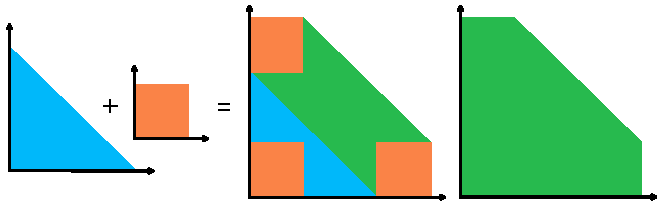
\includegraphics{part_2/chapter_2/figures/mink_sum}};
    		\node (A) at (-5, -0.5) {$S_1$};
    		\node (B) at (-2.9, -0.1) {$S_2$};
    		\node (C) at (-1, 1) {$S_2$};		
    		\node (D) at (-1, -1.1) {$S_2$};
    		\node (E) at (1.2, -1.1) {$S_2$};
    		\node (F) at (3, -0.5) {$S$};
    		\node (G) at (-1.1, -0.15) {$S_1$};
    	\end{tikzpicture}
		\caption{Minkowski sum of two convex sets.}\label{fig:mink_sum}
\end{figure}

%
\begin{figure}
	\centering
    \begin{tikzpicture}
%    		\draw[help lines] (-2,-2) grid (2,2);
    		\node (picture) at (0,0) {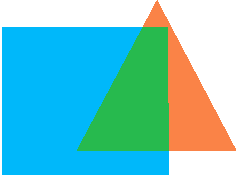
\includegraphics{part_2/chapter_2/figures/intersection.pdf}};
    		\node (A) at (-1, -0.15) {$S_1$};
    		\node (B) at (1.2, -0.5) {$S_2$};
    		\node (C) at (0.2, -0.8) {$S_1 \cap S_2$};
    \end{tikzpicture}
    
    \caption{Intersection of two convex sets.} \label{fig:intersection}
\end{figure}
%

\subsection{Examples of convex sets}

There are several familiar sets that are known to be convex. Having the knowledge that these sets are convex is useful as a building block for determining the convexity of more complicated sets.

Some important examples of convex sets include:
\begin{itemize}
	\item Them empty set $\emptyset$, any singleton $\{\overline{x}\}$ and the whole space $\reals^n$; 
	\item halfspaces: $S = \braces{x : p^\top x \leq \alpha} \subset \reals^n$;
	\item hyperplanes: $H = \braces{x : p^\top x = \alpha} \subset \reals^n$, where $p \neq 0^n$ is a normal vector and $\alpha\in \reals$ is a scalar. Notice that $H$ can be equivalently represented as $H = \braces{x \in \reals^n: p^\top(x - \overline{x}) = 0}$ for $\overline{x} \in H$;
	\item polyhedral sets: $P = \braces{x : Ax \leq b} \subset \reals^n$, where $A\in \reals^{m\times n}$ and $b \in \reals^n$;
	\item norm-induced sets (balls): $B = \braces{x : ||x - \overline{x}|| \leq \alpha} \subseteq \reals^n$, where $|| \cdot ||$ is any norm and $\alpha$ a scalar;
	\item norm cones: $C =\braces{(x,\alpha) \in \reals^{n+1}: ||x|| \leq \alpha} $;
\end{itemize} 

For example, let us consider the polyhedral set $P = \braces{x \in \reals^n : Ax \leq b} \subset \reals^n$ with $A$ being a $m \times n$ matrix. Notice that $S$ is the intersection of a collection of half-spaces $H_i = \braces{x \in \reals^n : a_i^\top x \leq b_i}$, where $a_i$ are vectors from the rows of the matrix $A$ and $b_i$ are the components of the column vector $b$. We know that $H_i$ are convex sets, thus $P = \cap_{i=1}^m H_i$ is also convex, as the intersection of sets is a convexity-preserving set operation.


\subsubsection{Hyperplanes and halfspaces}

Hyperplanes and halfspaces will play a central role in the developments we will see in our course. Therefore, let us take a moment and discuss some important aspects related these convex sets. First, notice that, geometrically, a hyperplane $H \subset \reals^n$ can be interpreted as the set of points with a \emph{constant} inner product to a given vector $p \in \reals^n$, while $\overline{x}$ determines the offset of the hyperplane from the origin. That is,
	\begin{equation*}
		H = \braces{x : p^\top(x - \overline{x}) = 0} \equiv \overline{x} + p^{\perp},
	\end{equation*}
	where $p^\perp$ is the orthogonal complement of $p$, i.e., the set of vectors orthogonal to $p$, which is given by $\braces{x \in \reals^n : p^\top x = 0}$.
	
	\begin{figure}[H]
	    \begin{tikzpicture}
%    		\draw[help lines] (-2,-2) grid (2,2);
    		\node (picture) at (0,0) {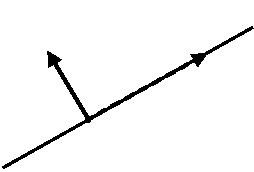
\includegraphics{part_2/chapter_2/figures/hyperplane.pdf}};
    		\node (p) at (-1.3, 0.8) {$p$};
    		\node (xbar) at (-0.6, -0.8) {$\overline{x}$};
    		\node (H) at (2, 0.5) {$H$};
		\end{tikzpicture}
		\caption{A hyperplane $H = \braces{x \in \reals^n: p^\top(x - \overline{x}) = 0}$ with normal vector $p$ displaced to $\overline{x}$.}
	\end{figure}
	
	Analogously, a halfspaces can be represented as $S = \braces{x \in \reals^n : p^\top(x - \overline{x}) \le 0}$ where $p^\top \overline{x} = \alpha$ is the hyperplane that forms the boundary of the halfspace. This definition suggests a simple geometrical interpretation: the halfspace $S$ consists of $\overline{x}$ plus any vector with an obtuse or right angle (i.e., greater of equal to 90$^\circ$) with the outward normal vector $p$.
 
 	\begin{figure}[H]
	    \begin{tikzpicture}
%    		\draw[help lines] (-2,-2) grid (2,2);
    		\node (picture) at (0,0) {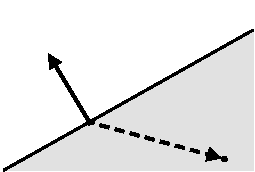
\includegraphics{part_2/chapter_2/figures/halfspace.pdf}};
    		\node (p) at (-1.3, 0.75) {$p$};
    		\node (xbar) at (-0.6, -0.9) {$\overline{x}$};
    		\node (x) at (1.9, -1.3) {$x$};
    		\node (H) at (1.7, 0.3) {$S$};
		\end{tikzpicture}
		\caption{A halfspace $S = \braces{x \in \reals^n : p^\top(x - \overline{x}) \le 0}$ defined by the same hyperplane $H$. Notice how the vectors $p$ (or $p - \overline{x}$, which is fundamentally the same vector but translated to $\overline{x}$) and $x - \overline{x}$ form angles greater or equal than $90^\circ$.}
	\end{figure}
	
	\begin{figure}[H]
    \begin{tikzpicture}
%    		\draw[help lines] (-2,-2) grid (2,2);
    		\node (picture) at (0,0) {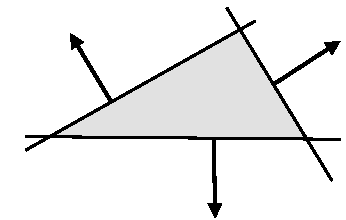
\includegraphics{part_2/chapter_2/figures/polyhedral_set.pdf}};
    		\node (P) at (0.75, 0.25) {$P$};
    		\node (a1) at (-1.6, 1.4) {$a_1$};
    		\node (a2) at (1, -1.8) {$a_2$};    		
    		\node (a2) at (2.8, 1.3) {$a_3$};
    \end{tikzpicture}
    \caption{A polyhedron $P$ formed by the intersection of three halfspace. Each hyperplane $H_i = \braces{x \in \reals^n : a_i^\top x \leq b_i}$, for $i = 1,2,3$, has a normal vector $a_i$, and has an offset from the origin $b_i$ (which cannot be seen once project on a 2-dimensional plane as in the picture).} \label{fig:polyhedral_set}
\end{figure}

\subsubsection{Norm balls and norm cones}

An Euclidean ball (or simply ball) of radius $\epsilon$ in $\reals^n$ has the form
%
\begin{equation*}
	B(\overline{x}, r) = \braces{x \in \reals^n : || x - \overline{x}||_2 \le \epsilon} \equiv \braces{x \in \reals^n : (x - \overline{x})^\top (x - \overline{x}) \le \epsilon^2}
\end{equation*}
%
As one might suspect, balls are convex, which can be proved by noting that
%
\begin{align*}
	||\lambda x_1 + (1 - \lambda) x_2 - \overline{x}||_2  & = ||\lambda (x_1 - \overline{x}) + (1 - \lambda) (x_2 - \overline{x})||_2 \\
	& \le \lambda ||x_1 - \overline{x}||_2 + + (1 - \lambda) ||x_2 - \overline{x}||_2 \le \epsilon.
\end{align*}
%
Notice that between the first and the second line, we use the triangle inequality, which states that $||x + y|| \le ||x|| + ||y||$ for any two vectors $x$ and $y$ and any norm (including the Euclidean norm). 

Euclidean balls are a special case of norm balls, which are defined as $B(\overline{x}, r) = \braces{x \in \reals^n : || x - \overline{x}|| \le \epsilon}$ where $||\ \cdot \ ||$ is any norm on $\reals^n$. 

A related set is the norm cone, defined as $C(x, \alpha) = \braces{(x,\alpha) \in \reals^{n+1} : ||x|| \le \alpha}$, where $\alpha$ is a scalar. For example, the second-order cone (also known as the ice cream cone or Lorentz cone) is the norm cone for the Euclidean norm.

\begin{remark} 
	Norm induced sets (balls or cones) are convex for any norm $||x||_p = \left(\sum_{i=1}^n x_i^p\right)^{\frac{1}{p}}$ for $x \in \reals^n$ and $p \geq 1$.
\end{remark}


\section{Convex hulls} 

A \emph{convex hull} of a set $S$, denoted $\conv(S)$ is the set formed by all convex combinations of all points in $S$. As the name suggests, $\conv(S)$ is a convex set, regardless of $S$ being or not convex. 

Another interpretation for $\conv(S)$ is to think of it as the tightest enveloping (convex) set that contains $S$. Notice that, if $S$ is convex, then $S = \conv(S)$.  Formally, convex hulls are defined as follows.

\begin{definition}[Convex hull of a set]\label{def: convex_hull}
	Let $S \subseteq \reals^n$ be an arbitrary set. The convex hull of $S$, denoted by $\conv(S)$, is the collection of all convex combinations of $S$. That is, for $x_j \in S$, with $j = 1,\dots, k$, $x \in \conv(S)$ if and only if 
	%
	\begin{equation*}
		x = \sum_{j=1}^k \lambda_jx_j : \sum_{j=1}^k \lambda_j = 1, \ \lambda_j \geq 0, \text{ for } j = 1,\dots,k.
	\end{equation*}                       
	%
\end{definition}
%

From Definition \ref{def: convex_hull}, one can show that the convex hull $\conv(S)$ can also be defined as the intersection of all convex sets containing $S$. Perhaps the easiest way to visualise this is to think of the infinitely many half-space containing $S$ and their intersection, which can only be $S$. Figure \ref{fig:convex_hull} illustrates the convex hull $\conv(S)$ of an nonconvex set $S$.
%
\begin{figure}[H]
%
\includegraphics[width=0.3\textwidth]{Figures/convex_hull.pdf}
	\begin{tikzpicture}
%    		\draw[help lines] (-3,-2) grid (3,2);
    		\node (picture) at (0,0) {
\includegraphics{part_2/chapter_2/figures/convex_hull.pdf}};
    		\node (A) at (-1.5, 0) {$S$};
    		\node (B) at (0.3, 0.5) {$\conv(S)$};
    \end{tikzpicture}
\caption{Example of an arbitrary set $S$ (in solid blue) and its convex hull $\conv(S)$ (combined blue and grey areas).} \label{fig:convex_hull}
\end{figure}
%
The notion of convex hulls is a powerful tool in optimisation. One important application is using $\conv(S)$ to obtain approximations for a nonconvex $S$ that can be exploited to solve an optimisation problem with constraint set defined by $S$. This is the underpinning technique in many important optimisation methods for such as branch-and-bound-based methods for nonconvex problems and decomposition methods (i.e., methods that solve large problems by breaking it into smaller parts that are presumably easier to solve).  

In specific, let us consider the convex hull of a finite collection of discrete points. Some of these sets are so important in optimisation that they have their own names. 
%
\begin{definition}
Let $S = \braces{x_1, \dots, x_{n+1}} \subset \reals^n$. Then $\conv(S)$ is called a \emph{polytope}. If $x_1,\dots,x_{n+1}$ are affinely independent (i.e., $x_2 - x_1, \dots ,x_{n+1} - x_1$ are linearly independent) then $\conv(S)$ is called a \emph{simplex} with vertices $x_1,\dots,x_{n+1}$.
\end{definition}
%


%\subsection{The Carath\'eodory theorem*}
%
%
%The \emph{Carath\'eodory theorem} is an important result associated with simplexes. It states that if $x \in \conv(S) \subset \reals^n$, then there exists a simplex composed by $x_j \in S$ for $j = 1, \dots, n+1$ that contains $x$. Formally, the theorem is posed as follows.
%%
%\begin{theorem}[Carath\'eodory theorem]
%Let $S \subseteq \reals^n$. If $x \in \conv(S)$, then $x \in \conv(x_1, \dots, x_{n+1})$ for some $x_j \in S$ where $j = 1,\dots, n+1$.        
%\end{theorem}   
%
%%% Consider including a proof for the Caratheodory theorem, for the sake of completeness.
%
%
%More specifically, any point $x \in \conv(S)$ can be expressed as
%%
%\begin{equation*}
%	x = \sum_{j=1}^{n+1} \lambda_jx_j : \sum_{j=1}^{n+1} \lambda_j = 1, \ \lambda_j \geq 0, \text{ for } j = 1,\dots,{n+1},
%\end{equation*}
%%
%for a given collection of points $x_j$, with $j = 1, \dots, n+1$ forming a simplex. Figure \ref{fig:caratheodory} illustrates this result.
%%
%\begin{figure}[h]
%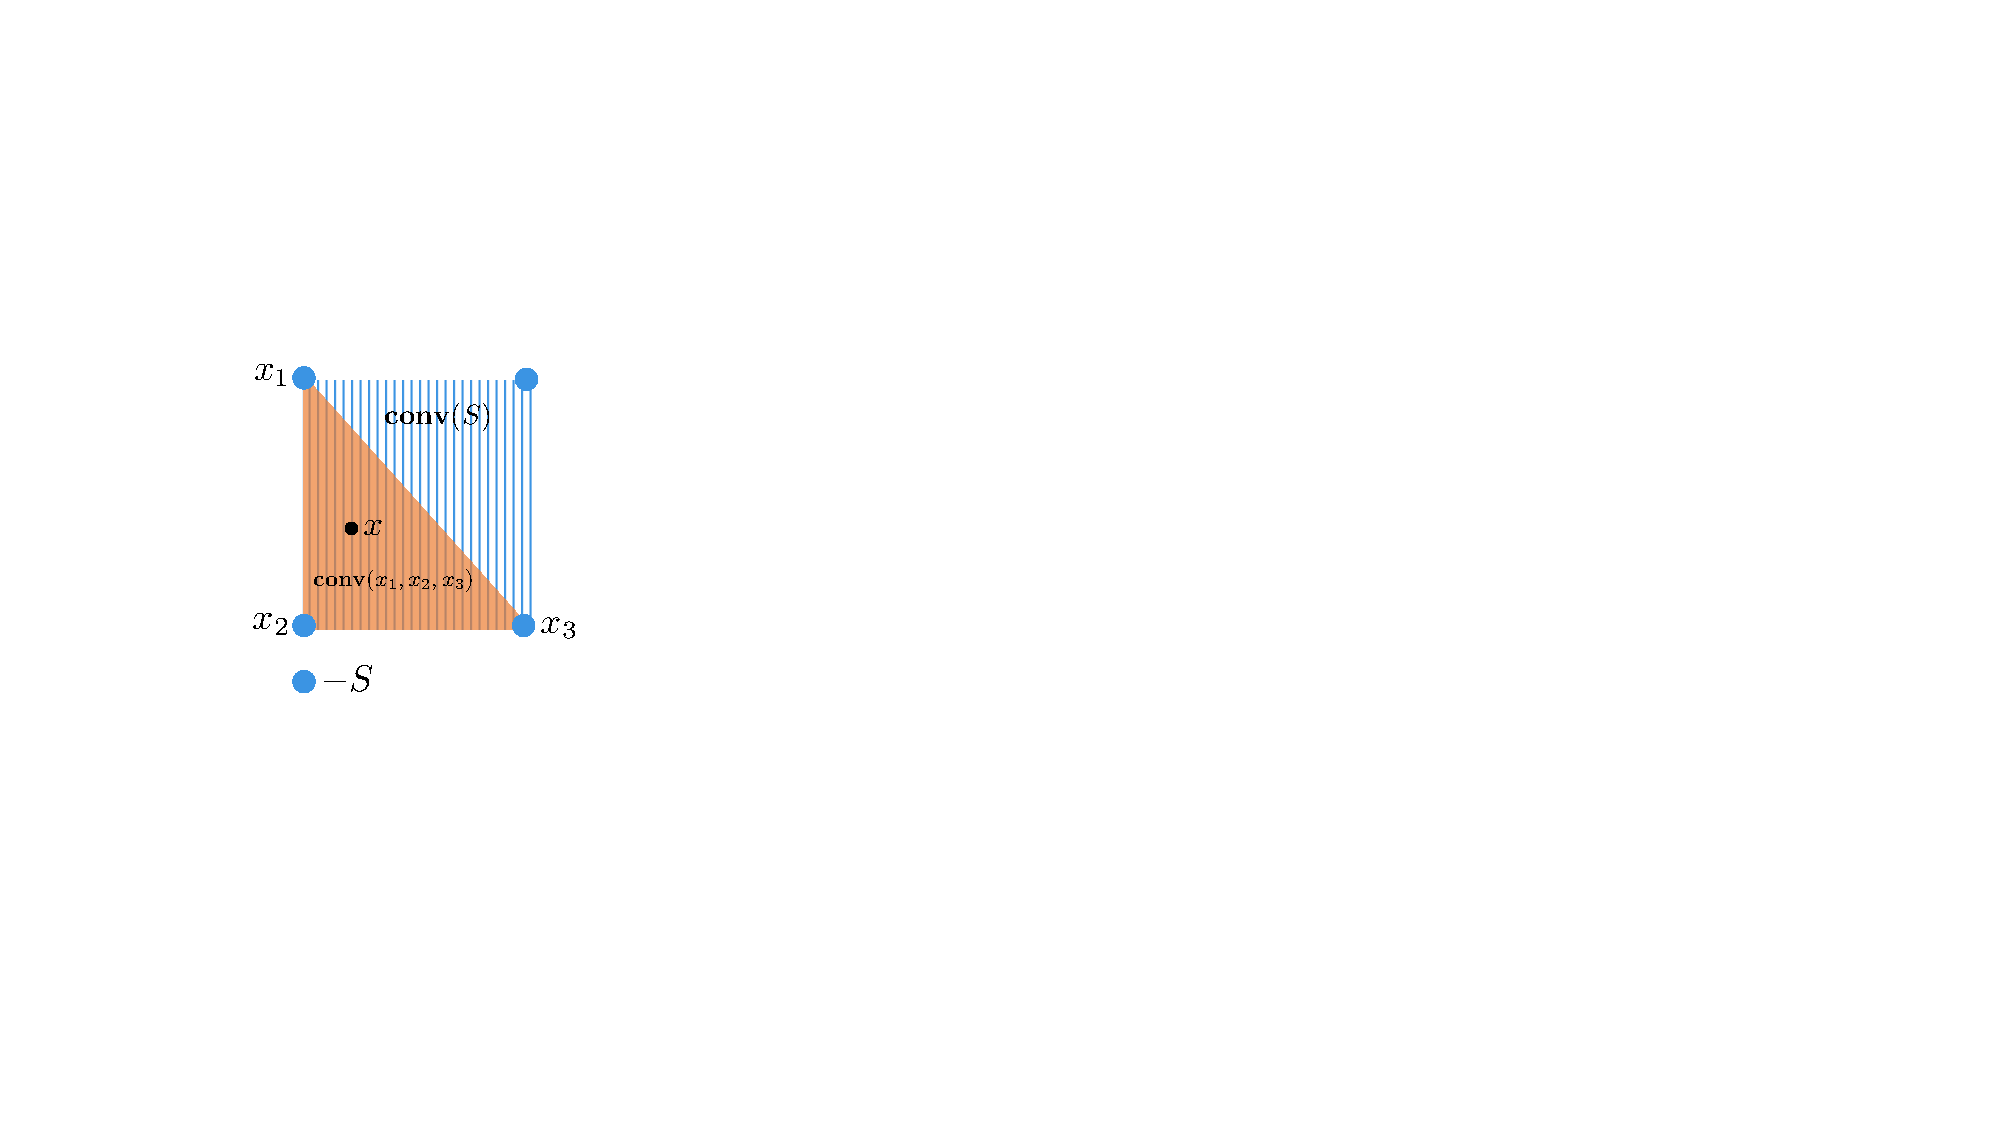
\includegraphics[width=0.3\textwidth]{Figures/caratheodory.pdf}
%\caption{Example of an arbitrary set $S$ (blue dots) and its convex hull $\conv(S)$ (light blue). Notice that $x$ can be represented as the convex combination of $x_j$ for $j=1,2,3$ for $n=2$.} \label{fig:caratheodory}
%\end{figure} 


\section{Closure and interior of sets}

Many of the set-related results we will see in this course depends on the characteristics of the set itself. Often, assuming properties such as closedness or compactness considerably ease technical derivations. 


\subsection{Closure, interior and boundary of a set}


Let us define some properties that will be useful in this course. For that, we will use an $\epsilon$-neighbourhood of $x \in \reals^n$ (which is a norm ball of radius $\epsilon$ centred in $x$) defined as
%
\begin{align*}
    N_\epsilon(x) = \braces{y : ||y - x|| < \epsilon}.
\end{align*}
%
Let $S \subseteq \reals^n$ be an arbitrary set. We can use $N_\epsilon$ to define the following elements related to $S$.  
\begin{enumerate}
\item \emph{Closure of $S$}: the set defined by the closure of $S$, denoted $\clo(S)$, is defined as 
%
\begin{align*}
\clo(S) = \braces{x \in \reals^n : S \cap N_\epsilon(x) \neq \emptyset \text{ for every } \epsilon > 0}. 
\end{align*}
%
Notice that the closure might contain points that do not belong to $S$. We say that a set is \emph{closed} if $S = \clo(S)$, that is, the set itself is its own closure. 
%
\item \emph{Interior of $S$}: the interior of $S$, denoted $\intr(S)$, is the set
\begin{align*}
\intr{S} = \braces{x \in S : N_\epsilon(x) \subset S \text{ for some } \epsilon > 0}.
\end{align*}
%
If $S$ is the same as its own interior, then we say that $S$ is \emph{open}. Some authors say that $S$ is solid if it has a nonempty interior (that is, $\intr(S) \neq \emptyset$. Notice that the interior of $S$ is a subset of $S$, that is $\intr(S) \subseteq S$.
%
\item \emph{Boundary of $S$}: the boundary of $S$, denoted $\bou(S)$ is the collection of points defined by
%
\begin{align*}
\bou(S) = \braces{x \in \reals^n : N_\epsilon(x) \text{ contains some } x_i \in S \text{ and some } x_j \notin S \text{ for every } \epsilon > 0}.
\end{align*}
%
We say that $S$ is bounded if exists $N_\epsilon(x)$, $x \in \reals^n$, for some $\epsilon > 0$ such that $S \subset N_\epsilon(x)$. 
\end{enumerate}

We say that a set is \emph{compact} if it is both \emph{closed} and \emph{bounded}. Compact sets appear very frequently in real-world applications of optimisation, since typically one can assume the existence of bounds for decision variables (such as nonnegativity or maximum physical bounds or, at an extreme case, smallest/ largest computational constants). Another frequent example of bounded set is the convex hull of a collection of discrete points, which is called by some authors \emph{polytopes} (effectively bounded polyhedral sets).  

Let us consider the following example. Let $S = \braces{(x_1,x_2) \in \reals^n : x_1^2 + x_2^2 \leq 1}$. Then, we have that:
\begin{enumerate}
	\item $\clo(S) = \braces{(x_1,x_2) \in \reals^n : x_1^2 + x_2^2 \leq 1}$. Since $S = \clo(S)$, $S$ is closed.
	\item $\intr(S) = \braces{(x_1,x_2) \in \reals^n : x_1^2 + x_2^2 < 1}$. 
	\item $\bou(S) = \braces{(x_1,x_2) \in \reals^n : x_1^2 + x_2^2 = 1}$. Notice that it makes $S$ bounded.
	\item $S$ is compact, since it is closed and bounded. 
\end{enumerate}

Notice that, if $S$ is closed, then $\bou(S) \subset S$. That is, its boundary is part of the set itself. Moreover, it can be shown that $\clo(S) = \bou(S) \cup S$ is the smallest closed set containing $S$. 

In case $S$ is convex, one can infer the convexity of the interior $\intr(S)$ and its closure $\clo(S)$. The following theorem summarises this result.
%
\begin{theorem}\label{thm:top_convex_comb}
Let $S \subseteq \reals^n$ be a convex set with $\intr(S) \neq \emptyset$. Let $x_1 \in \clo(S)$ and $x_2 \in \intr(S)$. Then $x = \lambda x_1 + (1 - \lambda) x_2 \in \intr(S)$ for all $\lambda \in (0,1)$.
\end{theorem}
%

% Consider including the proof for this theorem (on page 46)

Theorem \ref{thm:top_convex_comb} is useful for inferring the convexity of the elements related to $S$. We summarise the key results in the following corollary.
%
\begin{corollary} Let $S$ be a convex set with $\intr(S) \neq \emptyset$. Then
	\begin{enumerate}
		\item $\intr(S)$ is convex;
		\item $\clo(S)$ is convex;
		\item $\clo(\intr(S)) = \clo(S)$;
		\item $\intr(\clo(S)) = \intr(S)$.
	\end{enumerate}
\end{corollary}
%

% Consider including the proof for this corollary (on page 46)


\subsection{The Weierstrass theorem}


The Weierstrass theorem is a result that guarantees the existence of optimal solutions for optimisation problems. To make it more precise, let
%
\begin{align*}
	(P) :~ z = \mini\braces{f(x) : x \in S}  
\end{align*}
%
be our optimisation problem. If an optimal solution $x^*$ exists, then $f(x^*) \leq f(x)$ for all $x \in S$ and $z = f(x^*) = \min \braces{f(x) : x \in S}$. 

Notice the difference between $\mini$ (an abbreviation for minimise) and the operator $\min$. The first is meant to represent the problem of minimising the function $f$ in the domain $S$, while $\min$ is shorthand for minimum, in this case $z$, assuming that it is attainable.

It might be that an optimal solution is not attainable, but a bound can be obtained for the optimal solution value. The greatest lower bound for $z$ is its \emph{infimum} (or \emph{supremum} for maximisation problems), denoted by $\inf$. That is, if $z = \inf\braces{f(x) : x \in S}$ , then $z \leq f(x)$ for all $x \in S$ and there is no $\overline{z} > z$ such that $\overline{z} \leq f(x)$ for all $x \in S$. We might sometimes use the notation 
%
\begin{align*}
(P) :~ z = \inf\braces{f(x) : x \in S}
\end{align*}
%
to represent optimisation problems for which one cannot be sure whether an optimal solution is attainable. The Weierstrass theorem describes the situations in which those minimums (or maximums) are guaranteed to be attained, which is the case whenever $S$ is compact.
%
\begin{theorem}[Weierstrass theorem]\label{thm:weierstrass}
Let $S \neq \emptyset$ be a compact set, and let $f:S \rightarrow \reals$ be continuous on $S$. Then there exists a solution $\overline{x} \in S$ to $\mini\braces{f(x) : x \in S}$. 
\end{theorem}
%
Figure \ref{fig:Weierstrass} illustrates three examples. In the first (on the left) the domain $[a,b]$ is compact, and thus the minimum of $f$ is attained at $b$. In the other two, $[a,b)$ is open and therefore, Weierstrass theorem does not hold. In the middle example, one can obtain $\inf f$, which is not the case for the last example on the right.
%
\begin{figure}[h]
%\includegraphics[width=0.8\textwidth]{Figures/Weierstrass.pdf}
	\begin{tikzpicture}
%    		\draw[help lines] (-6,-1) grid (6,1);
    		\node (picture) at (0,0) {\includegraphics{part_2/chapter_2/figures/Weierstrass.pdf}};
    		\node (fa1) at (-5.8, 0.75) {$f(a)$};
    		\node (fb1) at (-5.8, -0.8) {$f(b)$};
 	    		\node (fa2) at (-1.8, 0.75) {$f(a)$};
    		\node (fb2) at (-1.8, -0.8) {$\inf f$};
 	    		\node (fa3) at (2.2, 0.75) {$f(a)$};
 	    		\node (a1) at (-5, -1.55) {$a$};
    		\node (b1) at (-3, -1.55) {$b$};
    		\node (a2) at (-1, -1.55) {$a$};
    		\node (b2) at (1, -1.55) {$b$};
 	    		\node (a3) at (3, -1.55) {$a$};
    \end{tikzpicture}
	\caption{Examples of attainable minimum (left) and infimum (centre) and an example where neither are attainable (right).} \label{fig:Weierstrass}
\end{figure}


\section{Separation and support of sets}
 

The concepts of \emph{separation} and \emph{support} of sets are key for establishing optimality conditions later in this course. We are interested in mechanisms that allow one to infer whether there exists hyperplanes separating points from sets (or sets from sets). We will also be interested in means to, given a point $x \notin S$, find the closest to point not belonging to $S$.

\subsection{Hyperplanes and closest points}

We start with how to identify closest points to sets. 
%
\begin{theorem}[Closest-point theorem]\label{thm:closest_point}
Let $S \neq \emptyset$ be a closed convex set in $\reals^n$ and $y \notin S$. Then, there exists a unique point $\overline{x} \in S$ with minimum distance from $y$. In addition, $\overline{x}$ is the minimising point if and only if $$(y-\overline{x})^\top(x - \overline{x}) \leq 0, \text{ for all } x\in S$$
\end{theorem}
%
Simply put, if $S$ is a closed convex set, then $\overline{x} \in S$ will be the closest point to $y \notin S$ if the vector $y - \overline{x}$ is such that if it forms an angle that is greater or equal than 90$^\circ$ with all other vectors $x - \overline{x}$ for $x \in S$. Figure \ref{fig:closest_point} illustrates this logic. 

\begin{figure}[h]
	\begin{tikzpicture}
%    	\draw[help lines] (-3,-2) grid (3,2);
		\node (picture) at (0,0) {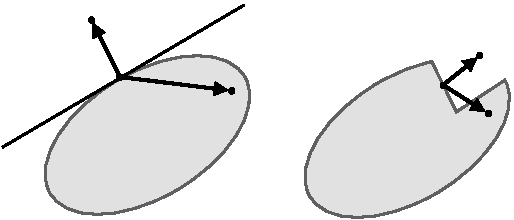
\includegraphics{part_2/chapter_2/figures/closest_point.pdf}};
		\node (y1) at (-2.8, 2) {$y$};
		\node (y2) at (4, 0.8) {$y$};
		\node (xbar1) at (-2.6, 0.4) {$\overline{x}$};
		\node (xbar2) at (2.9, 0.3) {$\overline{x}$};
		\node (x1) at (-0.4, -0.1) {$x$};    		
		\node (x2) at (3.9, -0.5) {$x$};
		\node (S) at (-2, -1) {$S$};
		\node (S) at (2, -1) {$S$};    		
    \end{tikzpicture}
	\caption{Closest-point theorem for a closed convex set (on the left). On the right, an illustration on how the absence of convexity invalidates the result.} \label{fig:closest_point}
\end{figure}

Notice that $S$ lies in the half-space $(y-\overline{x})^\top(x - \overline{x}) \leq 0$ defined by the hyperplane $p^\top(x - \overline{x}) =0$ with normal vector $p = (y - \overline{x})$. We will next revise the concepts of half-spaces and hyperplanes, since they will play a central role in the derivations in this course.  

\subsection{Halfspaces and separation}

We can use halfspaces to build the concept of separation. Let us start recalling that a hyperplane $H = \braces{x : p^\top x = \alpha}$ with normal vector $p \in \reals^n$ and $\alpha \in \reals$ defines two half-spaces $H^+ = \braces{x : p^\top x \geq \alpha}$ and $H^- = \braces{x : p^\top x \leq \alpha}$. Figure \ref{fig:hyperplane} illustrates the concept. Notice how the vector $p$ lies in the half-space $H^+$.
%
\begin{figure}
%	\includegraphics[scale=0.6]{Figures/hyperplanes.pdf}
	\begin{tikzpicture}
%    	\draw[help lines] (-2,-2) grid (2,2);
		\node (picture) at (0,0) {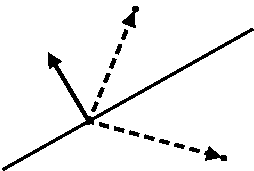
\includegraphics{part_2/chapter_2/figures/halfspaces.pdf}};
		\node (p) at (-1.4, 0.8) {$p$};
		\node (xbar) at (-0.7, -0.9) {$\overline{x}$};
		\node (H+) at (2, 1.2) {$H^{+}$};
		\node (H-) at (2, 0.5) {$H^{-}$};
	\end{tikzpicture}	
	\caption{Normal vectors, hyperplane and halfspaces} \label{fig:hyperplane}
\end{figure}
 
Any hyperplane $H$ can be defined in reference to a point $\overline{x} \in H$ by noticing that 
%
\begin{align*}
	p^\top(x - \overline{x}) = p^\top x - p^\top \overline{x} = \alpha - \alpha = 0.  
\end{align*}
%
From that, the half-spaces defined by $H$ can be equivalently stated as $H^+ = \braces{x : p^\top (x - \overline{x}) \geq 0}$ and $H^- = \braces{x : p^\top (x - \overline{x}) \leq 0}$.

We can now define the separation of convex sets. 
%
\begin{definition} \label{def:separation}
	Let $S_1$ and $S_2$ be nonempty sets in $\reals^n$. The hyperplane $H = \braces{x: p^\top x = \alpha}$ is said to \emph{separate} $S_1$ and $S_2$ if $ p^\top x \geq \alpha$ for each $x \in S_1$ and $p^\top x \leq \alpha$ for each $x \in S_2$. In addition, the following apply: 
	\begin{enumerate}
		\item {\bf Proper separation:} $S_1 \cup S_2 \not\subset H$;
		\item {\bf Strict separation:} $ p^\top x < \alpha$ for each $x \in S_1$ and $p^\top x > \alpha$ for each $x \in S_2$;
		\item {\bf Strong separation:} $ p^\top x \geq \alpha + \epsilon$ for some $\epsilon >0$ and $x \in S_1$, and $p^\top x \leq \alpha$ for each $x \in S_2$.
	\end{enumerate}
\end{definition}
%
Figure \ref{fig:separation} illustrates the three types of separation in Definition \ref{def:separation}. On the left, proper separation is illustrated, which is obtained by any hyperplane that does not contain both $S_1$ and $S_2$, but that might contain points from either or both. In the middle, sets $S_1$ and $S_2$ belong to two distinct half-spaces in a strict sense. On the right, strict separation holds with an additional margin $\epsilon > 0$, which is defined as strong separation. 
%
\begin{figure}[H]
%	\includegraphics[scale=0.8]{Figures/separations.pdf}
	\begin{tikzpicture}
%    	\draw[help lines] (-4,-2) grid (4,2);
		\node (picture) at (0,0) {\includegraphics{part_2/chapter_2/figures/separations.pdf}};
		\node (S11) at (-3.6, 0.5) {$S_1$};
		\node (S21) at (-3.15, -0.45) {$S_2$};
		\node (S12) at (-0.2, 0.5) {$S_1$};
		\node (S22) at (0.25, -0.45) {$S_2$};
		\node (S13) at (3, 0.5) {$S_1$};
		\node (S23) at (3.65, -0.45) {$S_2$};
		\node (H1) at (-2, 1.1) {$H$};		
		\node (H2) at (1.3, 1.1) {$H$};
		\node (H3) at (4.7, 1.1) {$H$};
	\end{tikzpicture}	
	\caption{Three types of separation between $S_1$ and $S_2$.} \label{fig:separation}
\end{figure}
%
A powerful yet simple result that we will use later is that, for a closed convex set $S$, there always exists a hyperplane separating $S$ and a point $y$ that does not belong to $S$.
%4
\begin{theorem}[Separation theorem]\label{thm:separation}
Let $S \neq \emptyset$ be a closed convex set in $\reals^n$ and $y \notin S$. Then, there exists a nonzero vector $p \in \reals^n$ and $\alpha \in \reals$ such that $p^\top x \leq \alpha$ for each $x \in S$ and $p^\top y > \alpha$.
\end{theorem}
%
\begin{proof}
	Theorem \ref{thm:closest_point} guarantees the existence of a unique minimising $\overline{x} \in S$ such that $(y-\overline{x})^\top(x - \overline{x}) \leq 0$ for each $x \in S$. Let $p = (y - \overline{x}) \neq 0$ and $\alpha = \overline{x}^\top(y - \overline{x}) = p^\top\overline{x}$. Then we get $p^\top x \leq \alpha$ for each $x \in S$, while $p^\top y - \alpha = (y - \overline{x})^\top(y - \overline{x}) = ||y - \overline{x}||^2 > 0$.
\end{proof}

This is the first proof we look at in these notes, and the reason for that is its importance in many of the results we will discuss further. The proof first looks at the problem of finding a minimum distance point as an optimisation problem and uses the Weierstrass theorem (our Theorem \ref{thm:closest_point} is a consequence of the Weierstrass theorem stated in Theorem \ref{thm:weierstrass}) to guarantee that such a $\overline{x}$ exists. Being a minimum distance point, we know from Theorem \ref{thm:closest_point} that $(y-\overline{x})^\top(x - \overline{x}) \leq 0$ holds. Now by defining $p$ and $\alpha$ as in the proof, one might notice that
%
\begin{align*}
	& (y-\overline{x})^\top(x - \overline{x}) \leq 0 \ \Leftrightarrow \ 
	(y-\overline{x})^\top x \leq (y - \overline{x})^\top\overline{x} \ \Leftrightarrow \ 
	p^\top x \leq p^\top\overline{x} = \alpha. 
\end{align*}
%
The inequality $p^\top y > \alpha$ is demonstrated to hold in the final part by noticing that 
%
\begin{align*}
	p^\top y - \alpha &= 
	(y - \overline{x})^\top y - \overline{x}^\top(y - \overline{x}) \\ &= 
	y^\top(y - \overline{x}) - \overline{x}^\top(y - \overline{x}) \\ & = (y - \overline{x})^\top (y - \overline{x}) = || y - \overline{x} ||^2 > 0.
\end{align*}

Theorem \ref{thm:separation} has interesting consequences. For example, one can apply it to every point in the boundary $\bou(S)$ to show that $S$ is formed by the intersection of all half-spaces containing $S$. 

Another interesting result is the existence of strong separation. If $y \notin \clo(\conv(S))$, then one can show that strong separation between $y$ and $S$ exists since there will surely be a distance $\epsilon>0$ between $y$ and $S$. 


\subsection{Farkas' theorem}

Farkas' theorem plays a central role in deriving optimality conditions. It can assume several alternative forms, which are typically referred to as Farkas' lemmas. In essence, the Farkas' theorem is used to demonstrate that a given system of linear equations has a solution if and only if a related system can be shown to have no solutions and vice-versa. 

\begin{theorem}
	Let $A$ be an $m \times n$ matrix and $c$ be an $n$-vector. Then exactly one of the following two systems has a solution:
	%
	\begin{align*}
		(1) :~ &Ax \leq 0, \ c^\top x > 0, \ x \in \reals^n\\
		(2) :~ &A^\top y = c, \ y \geq 0, \ y \in \reals^m.  
	\end{align*}
	%
\end{theorem}

\begin{proof}
	Suppose $(2)$ has a solution. Let $x$ be such that $Ax \leq 0$. Then $c^\top x = (A^\top y)^\top x = y^\top Ax \leq 0$. Hence, $(1)$ has no solution. 
	
	Next, suppose $(2)$ has no solution. Let $S = \braces{x \in \reals^n : x = A^\top y, \ y \geq 0}$. \hspace{-3pt}Notice that $S$ is closed and convex and that $c \notin S$. By Theorem \ref{thm:separation}, there exists $p \in \reals^n$ and $\alpha \in \reals$ such that $p^\top c > \alpha$ and $p^\top x \leq \alpha$ for $x \in S$. 
	
	As $0 \in S$, $\alpha \geq 0$ and $p^\top c > 0$. Also, $\alpha \geq p^\top A^\top y = y^\top Ap$ for $y \geq 0$. This implies that $Ap \leq 0$, and thus $p$ satisfies $(1)$. 
\end{proof}

The first part of the proof shows that, if we assume that system (2) has a solution, than $c^\top x > 0$ cannot hold for $y \geq 0$. The second part uses the separation theorem (Theorem \ref{thm:separation}) to show that $c$ can be seen as a point not belonging to the closed convex set $S$ for which there is a separation hyperplane and that the existence of such plane implies that system (1) must hold. The set $S$ is closed and convex since it is a conic combination of rows $a_i$, for $i=1, \dots, m$. Using the $0 \in S$, one can show that $\alpha \geq 0$. The last part uses the identity $p^\top A^\top  = (Ap)^\top$ and the fact that $(Ap)^\top y = y^\top Ap$. Notice that, since $y$ can be arbitrarily large and $\alpha$ is a constant, $y^\top Ap \leq \alpha$ can only hold if $y^\top Ap \leq 0$, requiring that $p \leq 0$ since $y \geq 0$ from the definition of $S$.

Farkas' theorem has an interesting geometrical interpretation arising from this proof, as illustrated in Figure \ref{fig:farkas}. Consider the cone $C$ formed by the rows of $A$
%
\begin{align*} 
	C = \braces{c \in \reals^n : c_j = \sum_{i=1}^m a_{ij} y_i, \ j= 1,\dots,n, \  y_i \geq 0, \ i =1,\dots, m}
\end{align*}
%
The \emph{polar cone} of $C$, denoted $C^0$, is formed by the all vectors having angles of 90$^\circ$ or more with vectors in $C$. That is, 
%
\begin{align*}
	C^0 = \braces{x : Ax \leq 0}.
\end{align*}
%
Notice that $(1)$ has a solution if the intersection between the polar cone $C^0$ and the positive ($H^+$ as defined earlier) half-space $H^+ = \braces{x \in \reals^n: c^\top x > 0}$ is not empty. If $(2)$ has a solution, as in the beginning of the proof, then $c \in C$ and the intersection $C^0 \cap H^+ = \emptyset$. Now, if $(2)$ does not have a solution, that is, $c \notin C$, then one can see that $C^0 \cap H^+$ cannot be empty, meaning that $(1)$ has a solution.  

\begin{figure}[h]
%	\includegraphics[width = 0.7\textwidth]{Figures/farkas.pdf}
	\begin{tikzpicture}
%    	\draw[help lines] (-5,-2) grid (5,2);
		\node (picture) at (0,0) {\includegraphics{part_2/chapter_2/figures/farkas.pdf}};
		\node (C01) at (-4,-0.5) {$C_0$};
		\node (C01) at (1.5,-0.7) {$C_0$};
		\node (C1) at (-1.5,-0.5) {$C$};
		\node (C2) at (4,-0.5) {$C$};
		\node (c1) at (-1.4,0) {$c$};
		\node (c2) at (2,1.7) {$c$};			
		\node (a11) at (-1.7,2) {$a_1$};
		\node (a12) at (3.8,2) {$a_1$};
		\node (a21) at (-0.8,1) {$a_2$};
		\node (a12) at (4.7,1) {$a_2$};
		\node (a31) at (-0.4,-1.3) {$a_3$};
		\node (a31) at (5.1,-1.3) {$a_3$};
	\end{tikzpicture}
	\caption{Geometrical illustration of the Farkas' theorem. On the left, system $(2)$ has a solution, while on the right, system $(1)$ has a solution} \label{fig:farkas}
\end{figure}


\subsection{Supporting hyperplanes}

There is an important connection between the existence of hyperplanes that support a whole set and optimality conditions of points. Let us first define supporting hyperplanes. 

\begin{definition}[Supporting hyperplane]
	Let $S \neq \emptyset$ be a set in $\reals^n$, and let $\overline{x} \in \bou(S)$. $H = \braces{x \in \reals^n : p^\top (x-\overline{x}) =0}$ is a supporting hyperplane of $S$ at $\overline{x}$ if either $S \subseteq H^+$ (i.e., $p^\top (x-\overline{x}) \geq 0$ for $x \in S$) or $S \subseteq H^-$.  
\end{definition}

Figure \ref{fig:support_hyperplane} illustrates the concept of supporting hyperplanes. Notice that supporting hyperplanes might not be unique, with the geometry of the set $S$ playing an important role in that matter. 

Let us define the function $f(x) = p^\top x$ with $x \in S$. One can see that the optimal solution $\overline{x}$ given by 
%
\begin{align*}
	\overline{x} = \argmax_{x \in S} f(x)
\end{align*}
%
is a point $x \in S$ for which $p$ is a supporting hyperplane. A simple geometric analogy is to think that the $f$ increases value as one moves in the direction of $p$. The constraint $x \in S$ will eventually prevent the movement further from $S$ and this last contact point is precisely $\overline{x}$. This is a useful concept for optimising problem using gradients of functions, as we will discuss later in the course.

\begin{figure}[h]
	%\includegraphics[width=0.9\textwidth]{Figures/support_hyperplane.pdf}
	\begin{tikzpicture}
%    	\draw[help lines] (-6,-2) grid (6,2);
		\node (picture) at (0,0) {\includegraphics{part_2/chapter_2/figures/support_hyperplane.pdf}};
		\node (S1) at (-4.3,-0.5) {$S$};
		\node (S2) at (-1,-0.5) {$S$};
		\node (S3) at (2.5,-0.5) {$S$};
		\node (xbar1) at (-3.6,-0.5) {$\overline{x}$};
		\node (xbar2) at (0.55,0.35) {$\overline{x}$};
		\node (p11) at (-3, -1.5) {$p$};		
		\node (p21) at (1.4, 0.75) {$p_1$};		
		\node (p22) at (1.6, 0.3) {$p_2$};
		\node (p31) at (4.3, 1.4) {$p$};
		\node (p32) at (5.05, 0.6) {$p$};
		\node (xbar31) at (3.52, 0.57) {$\overline{x}_1$};				
		\node (xbar32) at (4.25, -0.2) {$\overline{x}_2$};						
	\end{tikzpicture}
	\caption{Supporting hyperplanes for an arbitrary set. Notice how a single point might have multiple supporting planes (middle) or different points might have the same supporting hyperplane (right)} \label{fig:support_hyperplane} 
\end{figure}

One characteristic that convex sets present that will be of great importance when establishing optimality conditions is the existence of supporting hyperplanes at every boundary point.

\begin{theorem}[Support of convex sets]
	Let $S \neq \emptyset$ be a convex set in $\reals^n$, and let $\overline{x} \in \bou(S)$. Then there exists $p \neq 0$ such that $p^\top(x - \overline{x}) \leq 0$ for each $x \in \clo(S)$.
\end{theorem}

The proof follows immediately from Theorem \ref{thm:separation}, without explicitly considering a point $y \notin S$ and by noticing that $\bou(S) \subset \clo(S)$. Figure \ref{fig:support_convex} provides an illustration of the theorem. 

\begin{figure}[H]
%	\includegraphics[width=0.3\textwidth]{Figures/support_convex.pdf}
	\begin{tikzpicture}
%    	\draw[help lines] (-2,-2) grid (2,2);
		\node (picture) at (0,0) {\includegraphics{part_2/chapter_2/figures/support_convex.pdf}};
		\node (S) at (0.25,-0.5) {$S$};
		\node (S) at (-1,1.6) {$p$};
		\node (S) at (1.6, -0.1) {$\overline{x}$};
	\end{tikzpicture}
	\caption{Supporting hyperplanes for convex sets. Notice how every boundary point has at least one supporting hyperplane} \label{fig:support_convex}
\end{figure}


	
	\chapter{Convex functions}
	\section{Convexity in functions}

Now we turn our attention to identifying the convexity of functions. Consider the general problem
%
\begin{align*}
	(P) :~ \mini & f(x) \\
	\st          & g(x) \leq 0 \\
    	         & x \in X  
\end{align*}
% 
with $f:\reals^n \mapsto \reals$, $g: \reals^n \mapsto \reals^m$ and $X \subseteq \reals^n$. Assuming $X$ is a convex set, the next step towards attesting that $(P)$ is a convex problem is to check whether $f$ and $g$ are convex. It is important to emphasise (perhaps redundantly at this point) how crucial is for us to be able to attest the convexity $(P)$, since it allows us to generalise local optimality results to the whole domain of the problem.

The convexity of functions has a different definition than that used to define convex sets.
%
\begin{definition}[Convexity of a function I]\label{def:convex_function}
	Let $f:S \mapsto \reals$ where $S \subseteq \reals^n$ is a nonempty convex set. The function $f$ is said to be \emph{convex} on $S$ if
	$$ f(\lambda x_1 + (1-\lambda)x_2) \leq \lambda f(x_1) + (1-\lambda)f(x_2)
	$$
	for each $x_1, x_2 \in S$ and for each $\lambda \in [0,1]$.
\end{definition}
%
Very often, we use the term convex to loosely refer to  concave functions, which must be done with caution. In fact, if $f$ is convex, than $-f$ is concave and we say that $(P)$ is a convex problem even if $f$ is concave and we seek to maximise $f$ instead. Also, linear functions are both convex and concave. 

We say that a convex function is \emph{strictly convex} if the inequality holds strictly in Definition \ref{def:convex_function} for each $\lambda \in (0,1)$ (notice the open interval instead). In practice, it means that the function is guaranteed to not present flatness around its minimum (or maximum, for concave functions).

\subsection{Example of convex functions}

Some examples of convex function are:
%
\begin{enumerate}
	\item $f(x) = a^\top x + b$;
	\item $f(x) = e^x$;
	\item $f(x) = x^p$ on $\reals_+$ for $ p \leq 0$ or $p \geq 1$; concave for $0 \leq p \leq 1$.
	\item $f(x) = ||x||_p$ ($p$-norm);
	\item $f(x) = -\log x $ and negative entropy $f(x) = -x\log x $ are concave;
	\item $f(x) = \max\braces{x_1, \dots, x_n}$.
\end{enumerate}
%
Knowing that these common functions are convex is helpful for identifying convexity in more complex functions formed by \emph{composition}. By knowing that an operation between functions preserves convexity, we can infer the convexity of more complicated functions. The following are convexity preserving operations.
%
\begin{enumerate}
	\item Let $f_1, \dots, f_k : \reals^n \mapsto \reals$ be convex. Then these are convex:
	\begin{itemize}
		\item $f(x) = \sum_{j=1}^k\alpha_j f_j(x)$ where $\alpha_j >0$ for $j=1,\dots,k$;
		\item $f(x) = \max\braces{f_1(x), \dots, f_k(x)}$;
	\end{itemize}
		\item $f(x) = \frac{1}{g(x)}$ on $S$, where $g:\reals^n \mapsto \reals$ is concave and $S = \braces{x : g(x) > 0}$; 
		\item $f(x) = g(h(x))$, where $g: \reals \mapsto \reals$ is a nondecreasing convex function and $h:\reals^n \mapsto \reals$ is convex.
	\item $f(x) = g(h(x))$,\hspace{-1pt} where $g: \reals^m\hspace{-1pt} \mapsto\hspace{-1pt} \reals$ is convex and\hspace{-1pt} $h:\reals^n \mapsto \reals^m$ is affine: $h(x) = Ax + b$ with $A\in \reals^{m\times n}$ and $b\in \reals^m$.
\end{enumerate}


\subsection{Convex functions and their level sets}

There is a strong connection between convexity of sets and the convexity of functions. Let us first consider \emph{level sets}, which is one type of set spawned by functions. 

\begin{definition}[Lower level set]
	Let $S \subseteq \reals^n$\hspace{-1pt} be a nonempty set. The lower level set of $f: \reals^n \mapsto \reals$ for $\alpha \in \reals$ is given by
	%
	\begin{align*}
		S_\alpha = \braces{x \in S : f(x) \leq \alpha}.
	\end{align*}
	%
\end{definition}

Figure \ref{fig:sublevels} illustrates the lower level sets of two functions. The lower level set $S_\alpha$ can be seem as the projection of the function image onto the domain for a given level $\alpha$. 

\begin{figure}[H]
	\begin{tikzpicture}
%		\draw[help lines] (-6,-2) grid (6,2);
		\node (pic) at (0,0) {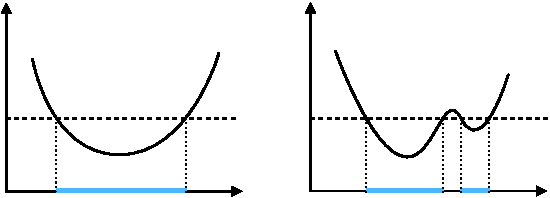
\includegraphics{part_2/chapter_3/figures/sublevels.pdf}};
		\node (fx1) at (-4,1.5) {$f(x)$};
		\node (fx2) at (1.2,1.5) {$f(x)$};
		\node (x1) at (-0.4,-1.7) {$x$};
		\node (x2) at (4.75,-1.7) {$x$};
		\node (alpha1) at (-4.8, -0.3) {$\alpha$};
		\node (alpha1) at (0.4, -0.3) {$\alpha$};
	\end{tikzpicture}
	\caption{The lower level sets $S_\alpha$ (in blue) of two functions, given a value of $\alpha$. Notice the nonconvexity of the level set of the nonconvex function (on the right)} \label{fig:sublevels}
\end{figure}

Notice that, for convex functions, no discontinuity can be observed, making $S_\alpha$ convex. Lemma \ref{lem:level_sets} states this property.

\begin{lemma}\label{lem:level_sets}
	Let $S \subseteq \reals^n$ be a nonempty convex set and $f:S \mapsto \reals$ a convex function. Then, any level set $S_\alpha$ with $\alpha \in \reals$ is convex. 
\end{lemma} 
%
\begin{proof}
	Let $x_1, x_2 \in S_\alpha$. Thus, $x_1, x_2 \in S$ with $f(x_1) \leq \alpha$ and $f(x_2) \leq \alpha$. Let $\lambda \in (0,1)$ and $x = \lambda x_1 + (1-\lambda)x_2$. Since $S$ is convex, we have that $x \in S$. Now, by the convexity of $f$, we have 
	$$ f(x) \leq \lambda f(x_1) + (1 - \lambda)f(x_2) \leq \lambda\alpha + (1 - \lambda)\alpha = \alpha
	$$
	and thus $x \in S_\alpha$.
\end{proof}

{\bf Remark:} notice that a convex lower level set does not necessarily mean that the function is convex. In fact, as we will see later, there are nonconvex functions that have convex level sets (the so-called quasiconvex functions).  

\subsection{Convex functions and their epigraphs}

\emph{Epigraphs}, on the other hand, can be used to show the convexity of functions. Let us first formally define epigraphs.
%
\begin{definition}[Ephigraph]
	Let $S \subseteq \reals^n$\hspace{-1pt} be a nonempty set and $f:S \mapsto \reals$.\hspace{-1pt} The epigraph of $f$ is $$ \epi(f) = \braces{(x, y) : x \in S, y \in \reals, y \geq f(x)} \subseteq \reals^{n+1}
$$
\end{definition}
%
Figure \ref{fig:epigraphs} illustrates the epigraphs of two functions. Notice that the second function (on the right) is not convex, and nor is its epigraph. In fact, we can use the convexity of epigraphs (and the technical results associated with the convexity of sets) to show the convexity of functions.
% 
\begin{figure}
	\begin{tikzpicture}
%		\draw[help lines] (-6,-2) grid (6,2);
		\node (pic) at (0,0) {	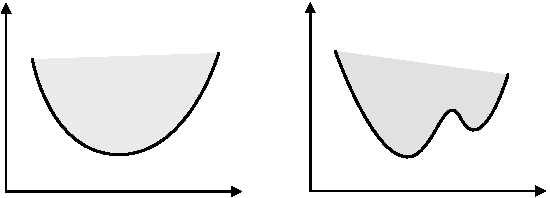
\includegraphics{part_2/chapter_3/figures/epigraphs.pdf}}; 		
		\node (fx1) at (-4,1.5) {$f(x)$};
		\node (fx2) at (1.2,1.5) {$f(x)$};
		\node (x1) at (-0.4,-1.7) {$x$};
		\node (x2) at (4.75,-1.7) {$x$};
		\node (epi1) at (-2.5, 0) {$\epi(f)$};				
		\node (epi2) at (2.5, 0.2) {$\epi(f)$};
	\end{tikzpicture}
	\caption{The epigraph $\epi()f$ of a convex function is a convex set (in grey on the left).}\label{fig:epigraphs}
\end{figure}
%
\begin{theorem}[Convex epigraphs]\label{thm:convex_epi}
	Let $S \subseteq \reals^n$ be a nonempty convex set and $f:S \mapsto \reals$. Then $f$ is convex if and only if $\epi(f)$ is a convex set.
\end{theorem}
%
\begin{proof}
	First, suppose $f$ is convex and let $(x_1, y_1), (x_2, y_2)$ $\in \epi(f)$ for $\lambda \in (0,1)$. Then
\begin{equation*}
	\lambda y_1 + (1-\lambda)y_2 \geq \lambda f(x_1) + (1-\lambda)f(x_2) \geq f(\lambda x_1 + (1- \lambda)x_2).
\end{equation*}
As $\lambda x_1 + (1-\lambda)x_2 \in S$, $(\lambda x_1 + (1-\lambda)x_2,\lambda y_1 + (1-\lambda)y_2) \in \epi(f)$.

Conversely, suppose $\epi(f)$ is convex. Therefore $x_1, x_2 \in S$: $(x_1,f(x_1))\in \epi(f)$, $(x_2,f(x_2)) \in \epi(f)$ and $(\lambda x_1 + (1-\lambda)x_2, \lambda f(x_1) + (1-\lambda)f(x_2)) \in \epi(f)$ for $\lambda \in (0,1)$, implying that $\lambda f(x_1) + (1-\lambda)f(x_2) \geq f(\lambda x_1 + (1-\lambda)x_2)$.
\end{proof}

The proof starts with the implication ``if $f$ is convex, then $\epi(f)$ is convex''. For that, it assumes that $f$ is convex and use the convexity of $f$ to show that any convex combination of $x_1$,$x_2$ in $S$ will also be in the $\epi(f)$, which is the definition of a convex set.

To prove the implication ``if $\epi(f)$ is convex, then $f$ is convex'', we define a convex combination of points in $\epi(f)$ and use the definition of $\epi(f)$ to show that $f$ is convex by setting $y = \lambda f(x_1) + (1 - \lambda)f(x_2)$ and $x = \lambda x_1 + (1-\lambda)x_2$.


\section{Differentiability of functions}


\subsection{Subgradients and supporting hyperplanes}


Subgradients can be understood as supporting hyperplanes at the boundary of function epigraphs. They can be seem as first-order local approximations of the function, which is often helpful information for optimisation methods when searching for directions of improvement.
%
\begin{definition}[Subgradients]
	Let $S \subseteq \reals^n$ be a nonempty convex set and $f:S \mapsto \reals$ a convex function. Then $\xi\in \reals^n$ is a \emph{subgradient} of $f$ at $\overline{x} \in S$ if
	\begin{align} 
	f(x) \geq f(\overline{x}) + \xi^\top(x - \overline{x}). \label{eq:subgradient_inequality}
	\end{align}
\end{definition}
%
Inequality \eqref{eq:subgradient_inequality} is called the \emph{subgradient inequality} and is going to be useful in several contexts later int his course. The set of subgradients $\xi$ of $f$ at $\overline{x}$ is the \emph{subdifferential} 
	$$
	\partial_f(\overline{x}) = \braces{\xi \in \reals^n : f(x) \geq f(\overline{x}) + \xi^\top(x - \overline{x})}.
	$$ 

Every convex function $f : S \mapsto \reals$ has at least one subgradient at any point $\overline{x}$ in the interior of the convex set $S$. Requiring that $\overline{x} \in \intr(S)$ allows us to disregard boundary points of $f$ where $\partial(\overline{x})$ might be empty. Theorem \ref{thm:exist_subgrad} presents this result.
%
\begin{theorem}\label{thm:exist_subgrad}
	Let $S \subseteq \reals^n$ be a nonempty convex set and $f:S \mapsto \reals$ a convex function. Then for all $\overline{x} \in \intr(S)$, there exists $\xi\in \reals^n$ such that
	$$ H = \braces{(x,y) : y = f(\overline{x}) + \xi^\top(x - \overline{x})}$$ supports $\epi(f)$ at $(\overline{x}, f(\overline{x}))$. In particular,
	$$f(x) \geq f(\overline{x}) + \xi^\top(x - \overline{x}), \forall x \in S.$$
\end{theorem}
%
The proof consists of directly applying Theorem \ref {thm:convex_epi} and then using the support of convex sets theorem (Theorem 14 in Lecture 2) to show that the subgradient inequality holds.

% Add the actual proof for this.

\subsection{Differentiability and gradients for convex functions} 


Let us first define differentiability of a function.
%
\begin{definition}
	Let $S \subseteq \reals^n$ be a nonempty set. The function $f:S \mapsto \reals$ is differentiable at $\overline{x} \in \intr(S)$ if there exists a vector $\nabla f(\overline{x})$, called a gradient vector, and a function $\alpha: \reals^n \mapsto \reals$ such that 
	$$
	f(x) = f(\overline{x}) + \nabla f(\overline{x})^\top(x - \overline{x}) + ||x-\overline{x}||\alpha(\overline{x};x-\overline{x})
	$$ 
	where $\lim_{x \mapsto \overline{x}}\alpha(\overline{x}; x - \overline{x})=0$. If this is the case for all $\overline{x} \in \intr(S)$, we say that the function is differentiable in $S$.
\end{definition}
%
Notice that this definition is based on the existence of first-order (Taylor series) expansion, with an error term $\alpha$. This definition is useful as it highlights the requirement that $\nabla f(\overline{x})$ exists and is unique at $\overline{x}$ since the gradient is given by $\nabla f(x) = \left[ \frac{\partial f(x)}{\partial x_i} \right]_i=1,\dots,n$. 

If $f$ is differentiable in $S$, then its subdifferential $\partial(x)$ is a singleton (a set with a single element) for all $x \in S$. This is shown in Lemma \ref{lem:singleton_subgradient}
%
\begin{lemma}\label{lem:singleton_subgradient}
	Let $S \subseteq \reals^n$ be a nonempty convex set and $f:S \mapsto \reals$ a convex function. Suppose that $f$ is differentiable at $\overline{x} \in \intr(S)$. Then $\partial_f(\overline{x}) = \braces{\nabla f(\overline{x})}$, i.e., the subdifferential $\partial_f(\overline{x})$ is a singleton with $\nabla f(\overline{x})$ as its unique element.
\end{lemma}
%
\begin{proof}
	From Theorem \ref{thm:exist_subgrad}, $\partial f(\overline{x}) \neq \emptyset$. Moreover, combining the existence of a subgradient $\xi$ and differentiability of $f$ at $\overline{x}$, we obtain:
	\begin{align}
	&f(\overline{x} + \lambda d) \geq f(\overline{x}) + \lambda \xi^\top d \label{1}\\
	&f(\overline{x} + \lambda d) = f(\overline{x}) + \lambda \nabla f(\overline{x})^\top d + \lambda ||d||\alpha(\overline{x}; \lambda d) \label{2}
	\end{align}
	Subtracting \eqref{2} from \eqref{1}, we get 
	$
	0 \geq \lambda(\xi - \nabla f(\overline{x}))^\top d -\lambda ||d||\alpha(\overline{x}; \lambda d).
	$
	Dividing by $\lambda > 0$ and letting $\lambda \mapsto 0^+$, we obtain $(\xi - \nabla f(\overline{x}))^\top d \leq 0$. Now, by setting $d = \xi - \nabla f(\overline{x})$, it becomes clear that $\xi = \nabla f(\overline{x})$.
\end{proof}

Notice that in the proof we use $\overline{x} + \lambda d$ to indicate that $x$ is in direction $d$, scaled by $\lambda > 0$. The fact that $\partial_f(x)$ is a singleton comes from the uniqueness of the solution for $(\xi - \nabla f(\overline{x}))^\top(\xi - \nabla f(\overline{x})) = 0$.

Figure \ref{fig:subgradients} illustrates subdifferential sets for three distinct points of a piecewise linear function. The picture schematically represents a multidimensional space $x$ as a one-dimensional projection (you can imagine this picture as being a section in one of the $x$ dimensions). For the points in which the function is not differentiable, the subdifferential set contains an infinite number of subgradients. At points in which the function is differentiable (any mid-segment point) the subgradient is unique (a gradient) and the subdifferential is a singleton.

	\begin{figure}
		\begin{tikzpicture}
%			\draw[help lines] (-3.5,-3) grid (4,3); 
			\node (pic) at (0,0) {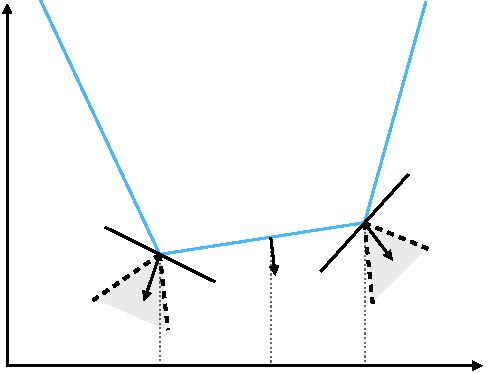
\includegraphics{part_2/chapter_3/figures/subgradients.pdf}};
			\node (fx) at (-4.5,3) {$f(x)$};
			\node (x) at (4.1,-3.2) {$x$};
			\node (xi1) at (-1.8,-2) {\footnotesize$\xi$};
			\node (xi2) at (2.55,-1.4) {\footnotesize$\xi$};
			\node (nablaf1) at (-2,-2.5) {$\partial f(x_1)$};
			\node (nablaf2) at (3,-1.9) {$\partial f(x_3)$};
			\node (nablaf3) at (0,-0.5) {\small$\partial f(x_2) = \nabla f(x_2)$};
			\node (x1) at (-1.4,-3.3) {$x_1$};
			\node (x2) at (0.5,-3.3) {$x_2$};
			\node (x3) at (2.1,-3.3) {$x_3$};	
		\end{tikzpicture}
		
		\caption{A representation of the subdifferential (in grey) for nondifferentiable ($x_1$ and $x_3$) and differentiable ($x_2$) points}\label{fig:subgradients}
	\end{figure}




If $f:S \mapsto \reals$ is a convex differentiable function, then Theorem \ref{thm:exist_subgrad} can be combined with Lemma \ref{lem:singleton_subgradient} to express the one of the most powerful results relating $f$ and its affine (first-order) approximation at $\overline{x}$.
%
\begin{theorem}[Convexity of a function II]\label{thm:convex_affine_bound}
	Let $S \subseteq \reals^n$ be a nonempty convex open set, and let $f:S \mapsto \reals$ be differentiable on $S$. The function $f$ is convex if and only if for any $\overline{x} \in S$, we have
	%
	\begin{align*}
		f(x) \geq f(\overline{x}) + \nabla f(\overline{x})^\top(x - \overline{x}), ~\forall x \in S.
	\end{align*}
\end{theorem}
%
The proof for this theorem follows from the proof for Theorem \ref{thm:exist_subgrad} to obtain the subgradient inequality and then use Lemma \ref{lem:singleton_subgradient} to replace the subgradient with the gradient. To see how the opposite direction (subgradient inequality holing implying the convexity of $f$), one should proceed as follows. 
\begin{enumerate}
	\item Take $x_1$ and $x_2$ from $S$. The convexity of $S$ implies that $\lambda x_1 + (1-\lambda)x_2$ is also in $S$.
	\item Assume that the subgradient exists, and therefore the two relations hold:
	%
	\begin{align}
		& f(x_1) \ge f(\lambda x_1 + (1-\lambda )x_2) + (1-\lambda )\xi^\top (x_1- x_2) \label{eq:conv1} \\
		& f(x_2) \ge f(\lambda x_1 + (1-\lambda )x_2) + \lambda \xi^\top (x_2- x_1) \label{eq:conv2}
	 \end{align}
	 \item Multiply \eqref{eq:conv1} by $\lambda$, \eqref{eq:conv2} by $(1-\lambda)$, and add them together. One will then obtain
	$$\lambda f(x_1) + (1-\lambda)f(x_2) \ge f(\lambda x_1 + (1-\lambda )x_2),$$ which is implies convexity.	 
\end{enumerate}



\subsection{Second-order differentiability}

 
We say that a function is \emph{twice-differentiable} if it has a second-order Taylor expansion. Having second-order expansions can be useful in that it allows for encoding curvature information in the approximation, which is characterised by the \emph{Hessian}, and to verify convexity (or strict convexity) by testing for semi-definiteness (positive definiteness).

Let $f_{ij}(\overline{x}) = \frac{\partial^2f(\overline{x})}{\partial x_i\partial x_j }$. Recall that the Hessian matrix  $H(\overline{x})$ at $\overline{x}$ is given by
%
\begin{align*}H(\overline{x}) = 
	\begin{bmatrix}
	f_{11}(\overline{x}) & \dots & f_{1n}(\overline{x})\\
	\vdots & \ddots & \vdots\\
	f_{n1}(\overline{x}) & \dots & f_{nn}(\overline{x})
	\end{bmatrix}
\end{align*}
%
Second-order differentiability can be defined as follows.
%
\begin{definition}[Second-order differentiability]
	Let $S \subseteq \reals^n$ be a nonempty set, and let $f:S \mapsto \reals$. Then $f$ is twice differentiable at $\overline{x} \in \intr(S)$ if there exists a vector $\nabla f(\overline{x})\in \reals^n$, an $n \times n$ symmetric matrix $H(\overline{x})$ (the Hessian), and a function $\alpha: \reals^n \mapsto \reals$ such that 
	\begin{align*}
	f(x) = f(\overline{x}) + \nabla f(\overline{x})^\top(x - \overline{x}) + 
	\frac{1}{2}(x - \overline{x})^\top H(\overline{x})(x - \overline{x}) + 
	||x-\overline{x}||^2\alpha(\overline{x};x-\overline{x})
	\end{align*}
	%
	where $\lim_{x \mapsto \overline{x}}\alpha(\overline{x}; x - \overline{x})=0$. If this is the case for all $\overline{x} \in S$, we say that the function is twice differentiable in $S$.
\end{definition}
%
We say that $H(\overline{x})$ is \emph{positive semi-definite} if $x^\top H(\overline{x})x \geq 0$ for $x \in \reals^n$. Having a positive semi-definite Hessian for all $x \in S$ implies that the function is convex in $S$. 
%
\begin{theorem}
	Let $S \subseteq \reals^n$ be a nonempty convex open set, and let $f:S \mapsto \reals$ be twice differentiable on $S$.\hspace{-4pt} Then\hspace{-1pt} $f$\hspace{-1pt} is convex if and only if the Hessian matrix is positive semidefinite (PSD) at each point in $S$.
\end{theorem}
%
\begin{proof}
Suppose $f$ is convex and let $\overline{x} \in S$. Since $S$ is open, $\overline{x} + \lambda x \in S$ for a small enough $|\lambda| \neq 0$. From Theorem \ref{thm:convex_affine_bound} and twice differentiability of $f$, we have 
%
\begin{align}
	&f(\overline{x} + \lambda x) \geq f(\overline{x}) + \lambda\nabla f(\overline{x})^\top x \label{3}\\ 
	&f(\overline{x} + \lambda x) =  f(\overline{x}) + \lambda \nabla f(\overline{x})^\top x + \frac{1}{2}\lambda^2 x^\top H(\overline{x})x + \lambda^2||x||^2\alpha(\overline{x};\lambda x) \label{4}
\end{align}
%
Subtracting \eqref{3} from \eqref{4}, we get 
$\frac{1}{2}\lambda^2x^\top H(\overline{x})x + \lambda^2||x||^2\alpha(\overline{x}; \lambda x) \geq 0$. Diving by $\lambda^2 > 0$ and letting $\lambda \rightarrow 0$, it follows that $x^\top H(\overline{x})x \geq 0$.

Conversely, assume that $H(\overline{x})$ is PSD for all $\overline{x} \in S$. Using the mean value theorem and second-order expansion, one can show that
%
\begin{align*}
	f(x) = f(\overline{x}) + \nabla f(\overline{x})^\top(x - \overline{x}) + \frac{1}{2}(x-\overline{x})^\top H(\hat{x})(x - \overline{x})
\end{align*}
%
where $\hat{x} = \lambda \overline{x} + (1-\lambda) x$ for $\lambda \in (0,1)$. Note that $\hat{x} \in S$ and $H(\hat{x})$ is positive semidefinite by assumption. Thus \hspace{-2pt}$(x-\overline{x})^\top H(\hat{x})(x - \overline{x}) \geq 0$, implying $f(x) = f(\overline{x}) + \nabla f(\overline{x})^\top(x - \overline{x}) \geq 0$.
\end{proof}
%
The proof uses a trick we have seen before. First, we assume convexity and use the definition of convexity provided by Theorem \ref{thm:convex_affine_bound} combined with an alternative definition for $(x - \overline{x})$ to show that $x^\top H(\overline{x})x \geq 0$. That is, instead of using the reference points $x$ and $\overline{x}$, we incorporate a step size $\lambda$ from $\overline{x}$ in the direction of $x$. 

To show the other direction of implication, that is, that $x^\top H(\overline{x})x \geq 0$ implies convexity, we use the \emph{mean value theorem}. The mean value theorem states that there must exist a point $\hat{x}$ between $x$ and $\overline{x}$ for which the second order approximation is exact. From these, we can derive the definition of convexity, as in Theorem \ref{thm:convex_affine_bound}.

Checking for positive semi-definiteness can be done efficiently using appropriate computational algebra method, though it can be computationally expensive. It involves calculating the eigenvalues of $H(\overline{x})$ and testing whether they are all nonnegative (positive), which implies the positive semi-definiteness (definiteness) of $H(\overline{x})$. Some nonlinear solvers are capable of returning warning messages (or errors even) pointing out lack of convexity by testing (under a certain threshold) for positive semi-definiteness.


\section{Quasiconvexity}

Quasiconvexity can be seem as the generalisation of convexity to functions that are not convex, but share similar properties that allow for defining global optimality conditions. One class of these functions are named \emph{quasiconvex}. Let us first technically define quasiconvex functions.
%
\begin{definition}[quasiconvex functions]
	Let $S \subseteq \reals^n$ be a nonempty convex set and $f:S \mapsto \reals$. Function $f$ is quasiconvex if, for each $x_1 ,x_2 \in S$ and $\lambda \in (0,1)$, we have
	\begin{align}
		f(\lambda x_1 + (1 - \lambda)x_2 ) \leq \max\braces{f(x_1), f(x_2)}. \label{eq:quasiconvexity}
	\end{align}
\end{definition}

We say that, if $f$ is quasiconvex, then $-f$ is quasiconcave. Also, functions that are both quasiconvex and quasiconcave are called \emph{quasilinear}. Quasiconvex functions are also called \emph{unimodal}.

Figure \ref{fig:quasiconvex} illustrates a quasiconvex function. Notice that, for any pair of points $x_1$ and $x_2$ in the domain of $f$, the graph of the function is always below the maximum between $f(x_1)$ and $f(x_2)$. This is precisely what renders convex the lower level sets of quasiconvex functions. Notice that, on the other hand, the epigraph $epi(f)$ is not a convex set. 

\begin{figure}[H]
		\begin{tikzpicture}
	%		\draw[help lines] (-6,-2) grid (6,2);
			\node (pic) at (0,0) {	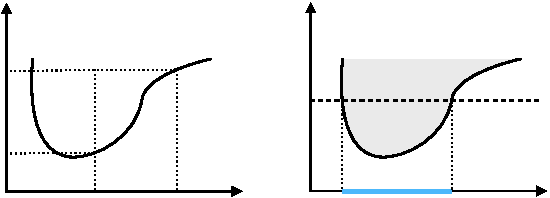
\includegraphics{part_2/chapter_3/figures/quasiconvex}}; 		
			\node (fx1) at (-4,1.5) {$f(x)$};
			\node (fx2) at (1.2,1.5) {$f(x)$};
			\node (x1) at (-0.4,-1.7) {$x$};
			\node (x2) at (4.75,-1.7) {$x$};
			\node (x11) at (-3, -1.8) {$x_1$};				
			\node (x21) at (-1.6, -1.8) {$x_2$};
	 		\node (fx11) at (-5.1, -0.9) {$f(x_1)$};
	  		\node (fx21) at (-5.1, 0.5) {$f(x_2)$};
	  		\node (fx21) at (0.3, 0) {$\alpha$};
	  		\node (fx21) at (2,-1.8) {$S_\alpha$};			
		\end{tikzpicture}
		\caption{A quasiconvex function with its epigraph (in grey) and lower level set (in blue).} \label{fig:quasiconvex}
	\end{figure}



Examples of quasiconvex functions include:
%
\begin{enumerate}
	\item $f(x) = \sqrt{|x|}$ in $\reals$
	\item $f(x) = \log x$ is quasilinear for $x > 0 $ 
	\item $f(x) = \inf\braces{z \in \integers : z \geq x}$ is quasilinear
	\item $f(x_1,x_2) = x_1x_2$ is quasiconcave on $S = \braces{(x_1, x_2) \in \reals^2 : x_1,x_2 > 0}$
\end{enumerate}
%
An important property of quasiconvex functions is that their level sets are convex. 
%
\begin{theorem}
	Let $S \subseteq \reals^n$ be a nonempty convex set and $f:S \mapsto \reals$. Function $f$ is quasiconvex if and only if $S_\alpha = \braces{x \in S: f(x) \leq \alpha}$ is convex for all $\alpha \in \reals$.
\end{theorem}
%
\begin{proof}
	Suppose $f$ is quasiconvex and let $x_1, x_2 \in S_\alpha$. Thus, $x_1, x_2 \in S$ and $\max\braces{f(x_1), f(x_2)} \leq \alpha$. Let $x = \lambda x_1 + (1-\lambda)x_2$ for $\lambda \in (0,1)$. As $S$ is convex, $x \in S$. By quasiconvexity of $f$, $f(x) \leq \max\braces{f(x_1), f(x_2)} \leq \alpha$. Hence, $x \in S_\alpha$ and $S_\alpha$ is convex.  

	Conversely, assume that $S_\alpha$ is convex for $\alpha \in \reals$. Let $x_1, x_2 \in S$, and let $x = \lambda x_1 + (1-\lambda)x_2$ for $\lambda \in (0,1)$. Note that, for $\alpha = \max\braces{f(x_1), f(x_2)}$, we have $x_1, x_2 \in S_\alpha$. The convexity of $S_\alpha$ implies that $x \in S_\alpha$, and thus $f(x) \leq \alpha = \max\braces{f(x_1), f(x_2)}$, which implies that $f$ is quasiconvex.
\end{proof}
 
The proof relies on the convexity of the domain $S$ to show that a convex combination from point in the level set $S_\alpha$ also belongs to $S_\alpha$. To show the other way around, we simply need to define $\alpha = \max\braces{f(x_1), f(x_2)}$ to see that a convex level set $S_\alpha$ implies that $f$ is quasiconvex. 

Quasiconvex functions have an interesting first-order condition that arises from the convexity of its level sets.

\begin{theorem}\label{thm:first-order_quasiconvex}
Let $S \subseteq \reals^n$ be a nonempty open convex set, and let $f:S \mapsto \reals$\lb be differentiable on $S$. Then $f$ is quasiconvex if and only if, for $x_1, x_2 \in S$ and $f(x_1) \leq f(x_2)$, $\nabla f(x_2)^\top(x_1 - x_2) \leq 0$.
\end{theorem}
%
\begin{figure}[h]
	\begin{subfigure}[b]{0.45\textwidth}
		\includegraphics[width=\textwidth]{part_2/chapter_3/figures/quasiconvex_surface.pdf}\caption{surface plot}\label{fig:quasiconvex_surface}
	\end{subfigure}
	\begin{subfigure}[b]{0.45\textwidth}
		\includegraphics[width=\textwidth]{part_2/chapter_3/figures/quasiconvex_contours.pdf}
	\caption{level curves}\label{fig:quasiconvex_contours}
	\end{subfigure}
	\caption{Surface plot and level curves for $f(x) = \sqrt{||x||_1}$} 
\end{figure}

The condition in Theorem \ref{thm:first-order_quasiconvex} is in fact sufficient for global optimality if one can show that $f$ is in fact \emph{strictly quasiconvex}, that is when \eqref{eq:quasiconvexity} holds strictly. Figure \ref{fig:quasiconvex_surface} and \ref{fig:quasiconvex_contours} show an example of a strict quasiconvex function and its level curves, illustrating that, despite the lack of convexity, the level sets are convex.

Strictly quasiconvex functions is a subset of a more general class of functions named \emph{pseudoconvex}, for which the conditions in Theorem \ref{thm:first-order_quasiconvex} are sufficient for global optimality. 
	
	\chapter{Unconstrained optimality conditions}
	\section{Recognising optimality}

We now turn our focus to recognising whether a given point satisfy necessary and/or sufficient conditions for optimality. Even though these conditions can be used to test if a candidate point is optimal for a problem, its most important use is serving as a framework for directing solution methods in their search for optimal solutions. 

Before we proceed, let us define the terminology we will use to refer to solutions. Let $f:\reals^n \mapsto \reals$. Consider the problem
$(P) :~ \mini\braces{f(x) : x \in S}$.
% 
\begin{enumerate}
\item a \emph{feasible solution} is any solution  $\overline{x} \in S$;
\item a \emph{local optimal solution} is a feasible solution $\overline{x}\in S$ that has a neighbourhood $N_\epsilon(\overline{x}) = \braces{x : ||x - \overline{x}|| \leq \epsilon}$ for some $\epsilon >0$ such that $f(\overline{x}) \leq f(x)$ for each $x \in S \cap N_\epsilon(\overline{x})$.
\item a \emph{global optimal solution} is a feasible solution $\overline{x} \in S$ with $f(\overline{x}) \leq f(x)$ for all $x \in S$. Or alternatively, is a local optimal solution for which $S \subseteq N_\epsilon(\overline{x})$.
\end{enumerate}
%
Figure \ref{fig:example_optima} illustrates the concepts above. Solution $x_1$ is an unconstrained global minimum, but is not a feasible solution considering the feasibility set $S$. Solution $x_2$ is a local optima, for any neighbourhood $N_\epsilon(x_2)$ only encompassing the points within the same plateau. Solution $x_3$ is a local optimum, while $x_4$ is neither a local or a global optimum in the unconstrained case, but is a global maximum in the constrained case. Finally, $x_5$ is the global minimum in the constrained case.

\begin{figure}
	\begin{subfigure}{\textwidth}
	\centering
		\begin{tikzpicture}
	%			\draw[help lines] (-5,-3) grid (5,3);
			\node (pic) at (0,0) {\includegraphics{part_2/chapter_4/figures/unconstrained.pdf}};
			\node (f) at (-4.3, 3.1) {$f(x)$};
			\node (x) at (5.1, -3) {$x$};
			\node (x1) at (-2.65,-3.2) {$x_1$};
			\node (x2) at (0.2,-3.2) {$x_2$};
			\node (x3) at (2.45,-3.2) {$x_3$}; 
			\node (x4) at (3.6,-3.2) {$x_4$}; 
		\end{tikzpicture}
		\caption{Unconstrained optimisation problem}\label{fig:unconstrained}	
	\end{subfigure}
	\begin{subfigure}{\textwidth}
	\centering
		\begin{tikzpicture}
%			\draw[help lines] (-5,-3) grid (5,3);
			\node (pic) at (0,0) {\includegraphics{part_2/chapter_4/figures/constrained.pdf}};
			\node (f) at (-4.3, 3.1) {$f(x)$};
			\node (x) at (5.1, -3) {$x$};
			\node (x1) at (-2.65,-3.2) {$x_1$};
			\node (x2) at (0.2,-3.2) {$x_2$};
			\node (x3) at (2.45,-3.2) {$x_3$}; 
			\node (x4) at (3.6,-3.2) {$x_4$};
			\node (x5) at (-2.1,-3.2) {$x_5$};
			\node (S) at (1.1,-2.5) {$S$}; 
		\end{tikzpicture}
		\caption{Constrained optimisation problem}\label{fig:constrained}		
	\end{subfigure}
	\caption{Points of interest in optimisation. Points $x_1$, $x_2$ and $x_3$ are local optima in the unconstrained problem. Once a constraint set $S$ is imposed, $x_4$ and $x_5$ become points of interest and $x_1$ becomes infeasible.} \label{fig:example_optima}		
\end{figure}


\section{The role of convexity in optimality conditions}


We can now state what is possibly the most important result in optimisation. In a nutshell, this results allows one promote local optimality to global optimality in the presence of convexity. 

\begin{theorem}[global optimality of convex problems]\label{thm:convex_global}
Let $S \subseteq \reals^n$ be a nonempty convex set and $f:S \mapsto \reals$ convex on $S$. Consider the problem $(P):~\mini \braces{f(x) : x \in S}$. Suppose $\overline{x}$ is a local optimal solution to $P$. Then $\overline{x}$ is a global optimal solution.
\end{theorem}

\begin{proof}
Since $\overline{x}$ is a local optimal solution, there exists $N_\epsilon(\overline{x})$ such that, for each $x \in S \cap N_\epsilon(\overline{x})$, $f(\overline{x}) \leq f(x)$. By contradiction, suppose $\overline{x}$ is not a global optimal solution. Then, there exists a solution $\hat{x} \in\hspace{-1pt} S$ so that $f(\hat{x}) < f(\overline{x})$. Now, for any $\lambda \in [0,1]$, the convexity of $f$ implies:  
%
\begin{align*}
f(\lambda\hat{x} + (1-\lambda)\overline{x}) \leq \lambda f(\hat{x}) + (1-\lambda)f(\overline{x}) < \lambda f(\overline{x}) + (1-\lambda)f(\overline{x}) = f(\overline{x})
\end{align*}
%
However, for $\lambda > 0$ sufficiently small, $\lambda\hat{x} + (1-\lambda)\overline{x} \in S\cap N_\epsilon(\overline{x})$ due to the convexity of $S$, which contradicts the local optimality of $\overline{x}$. Thus, $\overline{x}$ is a global optimum. 
\end{proof}

The proof is built using contradiction. That is, we show that for a solution to be a local optimum in a convex problem, not being a global solution contradicts its local optimality, originally true by assumption. This is achieved using the convexity of $f$ and showing that the convex combination between hypothetical better solution $\hat{x}$ and $\overline{x}$ would have to be both in $N_\epsilon(\overline{x})$ and better than $\overline{x}$, contradicting the local optimality of $\overline{x}$.


\section{Optimality condition of convex problems}


We first look at optimality conditions in a general sense to then translate the concept to unconstrained and constrained problems specifically. Taking this more general standpoint is also helpful to understand how these can be specialised in the absence of a closed domain or in the presence of differentiability. We assume convexity for now, and later we will discuss further the consequences of the absence of convexity. Note that unconstrained problems have convex feasibility set (i.e., the whole $\reals^n$), and thus what follows can be generalised to unconstrained optimisation problems.
%
\begin{theorem}[optimality condition for convex problems] \label{thm:opt_conditions}
Let $S \subseteq \reals^n$ be a nonempty convex set and $f:\reals^n \mapsto \reals$ convex on $S$. Consider the problem $(P) \,:\, \mini\braces{f(x) : x \in S}$.\hspace{-2pt} Then, $\overline{x}\in S$ is an optimal solution to $(P)$ if and only if $f$ has a subgradient $\xi$ at $\overline{x}$ such that $\xi^\top(x - \overline{x}) \geq 0$ for all $x \in S$. 
\end{theorem}  

\begin{proof}
Suppose that $\xi^\top(x-\overline{x}) \geq 0$ for all $x \in S$, where $\xi$ is a subgradient of $f$ at $\overline{x}$. By convexity of $f$, we have, for all $x \in S$
%
\begin{align*}
f(x) \geq f(\overline{x}) + \xi^\top(x - \overline{x}) \geq f(\overline{x})
\end{align*}
%
and hence $\overline{x}$ is optimal.

Conversely, suppose that $\overline{x}$ is a global optimal for $P$. Construct the sets:
%
\begin{align*}
&\Lambda_1 = \braces{(x - \overline{x},y) : x \in \reals^n, \ y > f(x) - f(\overline{x})} \\
&\Lambda_2 = \braces{(x - \overline{x},y) : x \in S, \ y \leq 0}
\end{align*}
%
Note that $\Lambda_1$ and $\Lambda_2$ are convex. By optimality of $\overline{x}$, $\Lambda_1 \cap \Lambda_2 = \emptyset$. Using the \emph{separation theorem}, there exists a hyperplane defined by $(\xi_0, \mu) \neq 0$ and $\alpha$ that separates $\Lambda_1$ and $\Lambda_2$:
%
\begin{align}
&\xi_0^\top(x - \overline{x}) + \mu y \leq \alpha, \ \forall x \in \reals^n, \ y > f(x) - f(\overline{x}) \label{h1}\\  
&\xi_0^\top(x - \overline{x}) + \mu y \geq \alpha, \ \forall x \in S, \ y \leq 0. \label{h2}
\end{align}
%
Letting $x = \overline{x}$ and $y=0$ in \eqref{h2}, we get $\alpha \leq 0$. Next, letting $x = \overline{x}$ and $y=\epsilon > 0$ in \eqref{h1}, we obtain $\alpha \geq \mu\epsilon$. As this holds for any $\epsilon > 0$, we must have $\mu \leq 0$ and $\alpha \geq 0$, the latter implying $\alpha = 0$.

If $\mu = 0$, we get from \eqref{h1} that $\xi_0^\top(x - \overline{x}) \leq 0$ for all $x\in \reals^n$. Now, by letting $x = \overline{x} + \xi_0$, it follows that $\xi_0^\top(x - \overline{x})  = ||\xi_0||^2 \leq 0$, and thus $\xi_0=0$. Since $(\xi_0, \mu) \neq 0$, we must have $\mu < 0$. 

Dividing \eqref{h1} and \eqref{h2} by $-\mu$ and denoting $\xi = \frac{-\xi_0}{\mu}$, we obtain:
%
\begin{align}
&\xi^\top(x - \overline{x}) \leq y, \ \forall x \in \reals^n, \ y > f(x) - f(\overline{x}) \label{h3}\\  
&\xi^\top(x - \overline{x}) \geq y, \ \forall x \in S, \ y \leq 0 \label{h4}
\end{align}
%
Letting $y=0$ in \eqref{h4}, we get $\xi^\top(x - \overline{x}) \geq 0$ for all $x \in S$. From \eqref{h3}, we can see that $y > f(x) - f(\overline{x})$ and $y \geq \xi^\top(x - \overline{x})$.\hspace{-2pt} Thus, $f(x) - f(\overline{x}) \geq \xi^\top(x - \overline{x})$, which is the \emph{subgradient inequality}. Thus, $\xi$ is a subgradient at $\overline{x}$ with $\xi^\top(x - \overline{x}) \geq 0$ for all $x \in S$.
\end{proof}
%
In the first part of the proof, we use the definition of convexity based on the subgradient inequality to show that $\xi^\top(x - \overline{x}) \geq 0$ implies that $f(\overline{x}) \leq f(x)$ for all $x \in S$. The second part of the proof uses the separation theorem in a creative way to show that the subgradient inequality must hold if $\overline{x}$ is optimal. This is achieved by using the two sets $\Lambda_1$ and $\Lambda_2$. Notice that, $\overline{x}$ being optimal implies that $y > f(x) - f(\overline{x}) \geq 0$, which leads to the conclusion that $\Lambda_1 \cap \Lambda_2 = \emptyset$, demonstrating the existence of a separating hyperplane between them, as shown in \eqref{h1} and \eqref{h2}. We can show that $\alpha$ in those has to be $0$ by noticing that $\mu\epsilon \leq 0$ must hold for $\epsilon > 0$ to be a bounded constant.

The second part is dedicated to show that $\mu < 0$, so we can divide \eqref{h1} and \eqref{h2} by $\mu$ to obtain the subgradient inequality as we have seen. We show that by contradiction, since $\mu =0$ would imply $\xi_0 = 0$, which disagrees with existence of a $(\xi, \mu) \neq 0$ in the separation theorem. Finally, as $y > f(x) - f(\overline{x})$ and $y \geq \xi^\top(x - \overline{x})$, for any given $y$, we have that $f(x) - f(\overline{x}) \geq \xi^\top(x - \overline{x})$ \footnote{Notice that, on the line of nonnegative reals, for a same $y$, $f(x) - f(\overline{x})$ is always on the 'right side' of $\xi^\top(x - \overline{x})$ because it is an open interval.}, which leads to the subgradient inequality. 

Notice that this result provides necessary and sufficient conditions for optimality for convex problems. These conditions can be extended to the unconstrained case as well, which is presented in Corollary \ref{cor:opt_conditions_open}.
%
\begin{corollary}[optimality in open sets] \label{cor:opt_conditions_open}
Under the conditions of Theorem \ref{thm:opt_conditions}, if $S$ is open, $\overline{x}$ is an optimal solution to $P$ if and only if $0 \in \partial f (\overline{x})$. 
\end{corollary}
%
\begin{proof}
From Theorem \ref{thm:opt_conditions}, $\overline{x}$ is optimal if and only if $\xi$ is a subgradient at $\overline{x}$ with $\xi^\top(x - \overline{x}) \geq 0$ for all $x \in S$. Since $S$ is open, $x = \overline{x} - \lambda\xi \in S$ for some $\lambda > 0$, and thus $-\lambda||\xi||^2 \geq 0$, implying $\xi = 0$.
\end{proof}
%
Notice that, if $S$ is open, then the only way to attain the condition $\xi^\top(x - \overline{x}) \geq 0$ is if $\xi = 0$ itself. This is particularly relevant in the context of nondifferentiable functions, as we will see later. Another important corollary is the classic optimality condition $\nabla f(\overline{x}) = 0$,  which we state below for completeness. 
%
\begin{corollary}[optimality for differentiable functions] \label{cor:opt_conditions_diff}
Suppose that $S \subseteq \reals^n$ is a nonempty convex set and $f:S \rightarrow \reals$ a differentiable convex function on $S$. Then $\overline{x} \in S$ is optimal if and only if $\nabla f(\overline{x})^\top (x - \overline{x}) \geq 0$ for all $x \in S$. Moreover, if $S$ is open, then $\overline{x}$ is optimal if and only if $\nabla f(\overline{x}) = 0$. 
\end{corollary}
%
The proof for Corollary \ref{cor:opt_conditions_diff} is the same as Theorem \ref{thm:opt_conditions} under a setting where $\partial (x) = \braces{\nabla f(x)}$ due to the differentiability of $f$.

Let us consider two examples. First, consider the problem

\begin{align*}
	\mini &\left(x_1 - \frac{3}{2}\right)^2 + (x_2 - 5)^2\\
	\st &-x_1 + x_2 \leq 2\\
	&2x_1 + 3x_2 \leq 11\\
	&x_1 \geq 0\\
	&x_2 \geq 0   
\end{align*}

Figure \ref{fig:ex_1} presents a plot of the feasible region $S$, which is form by the intersection of the two halfspaces, and the level curves of the objective function, with some of the values indicated in the curves. Notice that that this is a convex problem. 

\begin{figure}[H]
	\includegraphics{part_2/chapter_4/figures/ex1.pdf}
	\caption{Example 1}	\label{fig:ex_1}
\end{figure}

The arrow shows the gradient $\nabla f(\overline{x})$ at $\overline{x} = (1,3)$. Notice that this point is special since at that point, no vector $x - \overline{x}$ can be found forming an angle greater than 90$^\circ$ with $\nabla f(\overline{x})$, that is $\nabla f(\overline{x})^\top(x - \overline{x}) \geq 0$ for any $x \in S$, which means that $\overline{x}$ is optimal. Since the problem is convex, that is in fact the global optimum for this problem.

Figure \ref{fig:ex_2} shows a similar situation, but now with one of the constraints being nonlinear. Notice that of the two points highlighted ((1,2) in orange and (2,1) in purple), the optimality condition only holds for (2,1). For example, for $x = (2,1)$ and $\overline{x} = (1,2)$ the vector $x - \overline{x}$ forms a angle greater than 90$^\circ$ with the gradient of $f$ at $\overline{x}$, $\nabla f(\overline{x})$, and thus the condition $\nabla f(\overline{x})^(x - \overline{x}) \geq 0$ does not hold for all $S$. The condition does hold for $\overline{x} = (2,1)$, as can be seen in Figure \ref{fig:ex_2}.  

\begin{figure}[H]
	\includegraphics{part_2/chapter_4/figures/ex2.pdf}
	\caption{Example 2}	\label{fig:ex_2}
\end{figure}

A geometrical interpretation of the optimality condition $\xi^\top(x - \overline{x}) \geq 0$ is as follows. If there exists a subgradient $\xi$ (or a gradient $\nabla f(\overline{x})$ if $f$ is differentiable) that serves as a separating hyperplane between the level curve of $f$ at $\overline{x}$ and the feasible region $S$, then there can be no feasible point further into the lower level set defined by that level curve. Ultimately, this means that there is no feasible point with smaller objective function value to be found. This is why the separation theorem from Lecture 2 plays an important role here, since it can be used to state that the feasible options have been exhausted in terms of potential directions of decrease of objective function value.  

\subsection{Optimality conditions for unconstrained problems}

We have developed most of the concepts required to state optimality conditions for unconstrained optimisation problems, as presented in Corollaries \ref{cor:opt_conditions_open} and \ref{cor:opt_conditions_diff}. We now take an alternative route in which we do not take into account the feasibility set, but only the differentiability of $f$. This will be useful as it will allow us to momentarily depart from the assumption of convexity, which was used to state Theorem \ref{thm:opt_conditions}. 

\subsubsection{First-order optimality conditions}

Let us start defining what it means to be a \emph{descent direction}.

\begin{theorem}[descent direction]\label{thm:descent_dir}
Suppose $f: \reals^n \mapsto \reals$ is differentiable at $\overline{x}$. If there is $d$ such that $\nabla f(\overline{x})^\top d < 0$, there exists $\delta > 0$ such that $f(\overline{x} + \lambda d) < f(\overline{x})$ for each $\lambda \in (0, \delta)$, so that $d$ is a descent direction of $f$ at $\overline{x}$.
\end{theorem}
%
\begin{proof}
By differentiability of $f$ at $\overline{x}$, we have that 
\begin{align*}
\frac{f(\overline{x} + \lambda d)-f(\overline{x})}{\lambda} = \nabla f(\overline{x})^\top d + ||d||\alpha(\overline{x};\lambda d).
\end{align*}
Since $\nabla f(\overline{x})^\top d < 0$ and $\alpha(\overline{x};\lambda d) \rightarrow 0$ when $\lambda \rightarrow 0$ for some $\lambda \in (0, \delta)$, we must have $f(\overline{x} + \lambda d)-f(\overline{x}) < 0$.
\end{proof}

The proof uses the first-order expansion around $\overline{x}$ to show that, $f$ being differentiable, the condition $\nabla f(\overline{x})^\top d < 0$ implies that $ f(\overline{x} + \lambda d) < f(\overline{x})$, or put in words, that a step in the direction $d$ decreases the objective function value.

We can derive the first-order optimality condition in Corollary \ref{cor:opt_conditions_diff} as a consequence from Theorem \ref{thm:descent_dir}. Notice, however, that since convexity is not assumed, all we can say is that this condition is necessary (but not sufficient) for local optimality.

\begin{corollary}[first-order necessary condition]\label{thm:suff_first_order_cond}
Suppose $f: \reals^n \rightarrow \reals$ is differentiable at $\overline{x}$. If $\overline{x}$ is a local minimum, then $\nabla f(\overline{x}) = 0$.
\end{corollary}
%
\begin{proof}
By contradiction, suppose that $\nabla f(\overline{x}) \neq 0$. Letting $d = -\nabla f(\overline{x})$, we have that  $\nabla f(\overline{x})^\top d = -||\nabla f(\overline{x})||^2 < 0$. By Theorem \ref{thm:descent_dir}, there exists a $\delta > 0$ such that $f(\overline{x} + \lambda d) < f(\overline{x})$ for all $\lambda \in (0, \delta)$, thus contradicting the local optimality of $\overline{x}$. 
\end{proof}

Notice that Corollary \ref{thm:suff_first_order_cond} only holds in one direction. The proof uses contradiction once again, where we assume local optimality of $\overline{x}$ and show that having $\nabla f(\overline{x}) \neq 0$ contradicts the local optimality of $\overline{x}$, our initial assumption. To do that, we simply show that having any descent direction $d$ (we use $-\nabla f(\overline{x})$ since in this setting it is guaranteed to exist as $\nabla f(\overline{x}) \neq 0$) would mean that small step $\lambda$ can reduce the objective function value, contradicting the local optimality of $\overline{x}$. 


\subsubsection{Second-order optimality conditions}

We now derive necessary conditions for local optimality of $\overline{x}$ based on second-order differentiability. As we will see, it requires that the Hessian $H(\overline{x})$ of $f(x)$ at $\overline{x}$ is positive semidefinite.
%
\begin{theorem}[second-order necessary condition]\label{thm:second_order}
Suppose $f: \reals^n \rightarrow \reals$ is twice differentiable at $\overline{x}$. If $\overline{x}$ is a local minimum, then $H(\overline{x})$ is positive semidefinite.
\end{theorem}
%
\begin{proof}
Take an arbitrary direction $d$. As $f$ is twice differentiable, we have:
%
\begin{align*}
f(\overline{x} + \lambda d) = f(\overline{x}) + \lambda \nabla f(\overline{x})^\top d + \frac{1}{2}\lambda^ 2d^\top H(\overline{x}) d + \lambda^2||d||^2\alpha(\overline{x}; \lambda d)
\end{align*}
%
since $\overline{x}$ is a local minimum, Corollary \ref{thm:suff_first_order_cond} implies that $\nabla f(\overline{x})=0$ and $f(\overline{x} + \lambda d) \geq f(\overline{x})$. 

Rearranging terms and dividing by $\lambda^2 > 0$ we obtain
$$\frac{f(\overline{x} + \lambda d)-f(\overline{x})}{\lambda^2} =  \frac{1}{2}d^\top H(\overline{x}) d+ ||d||^2\alpha(\overline{x};\lambda d).
$$
Since $\alpha(\overline{x};\lambda d) \rightarrow 0$ as $\lambda \rightarrow 0$, we have that $d^\top H(\overline{x}) d \geq 0$.
\end{proof}

The second-order conditions can be used to attest local optimality of $\overline{x}$. In the case where $H(\overline{x})$ is positive definite, then this second order condition becomes \emph{sufficient} for local optimality, since it implies that the function is 'locally convex' for a small enough neighbourhood $N_\epsilon(\overline{x})$.

In case $f$ is convex, then the first-order condition $\nabla f(x) = 0$ becomes also sufficient for attesting the global optimality of $\overline{x}$. Recall that $f$ is convex if and only if $H(x)$ is positive semidefinite for all $x \in \reals^n$, meaning that in this case the second-order necessary conditions are also satisfied at $\overline{x}$.
%
\begin{theorem}
Let $f: \reals^n \mapsto \reals$ be convex. Then $\overline{x}$ is a global minimum if and only if $\nabla f(\overline{x}) = 0$.
\end{theorem}
%
\begin{proof}
From Corollary \ref{thm:suff_first_order_cond}, if $\overline{x}$ is a global minimum, then $\nabla f(\overline{x}) = 0$. Now, since $f$ is convex, we have that
%
\begin{align*}
f(x) \geq f(\overline{x}) + \nabla f(\overline{x})^\top (x - \overline{x})
\end{align*}
%
Notice that $\nabla f(\overline{x}) = 0$ implies that $\nabla f(\overline{x})^\top (x - \overline{x}) = 0$ for each $x \in \reals^n$, thus implying that $f(\overline{x}) \leq f(x)$ for all $x \in \reals^n$.
\end{proof}

	
	\chapter{Unconstrained optimisation methods: part 1}
	
\section{A prototype of an optimisation method}

Most, if not all, optimisation methods are based on the conceptual notion of successively obtaining \emph{directions} of potential improvement and suitable \emph{step sizes} in this direction, until a convergence or termination criterion (collectively called stopping criteria) is satisfied.

Considering what we have seen so far, we have now the concepts required for describing several unconstrained optimisation methods. We start by posing a conceptual optimisation algorithm in a pseudocode structure. This will be helpful in identifying the elements that differentiate the methods we will discuss.

%\captionsetup[algorithm]{font=footnotesize} 
\begin{algorithm}[H]
\caption{Conceptual optimisation algorithm} \label{Alg1}
\begin{algorithmic}[1] %line numbering frequency.
\State {\bf initialise.} iteration count $k = 0$, starting point $x_0$ 
\While {stopping criteria are not met} 
\State compute direction $d_k$ 
\State compute step size $\lambda_k $ %> 0$ 
\State $x_{k+1} = x_k + \lambda_k d_k$
\State $k = k+1$
\EndWhile
\State {\bf return} $x_k$.
\end{algorithmic}
\end{algorithm}

Algorithm \ref{Alg1} has two main elements, namely the computation of the direction $d_k$ and the step size $\lambda_k$ at each iteration $k$. In what follows, we present some univariate optimisation methods that can be employed to calculate step sizes $\lambda_k$. These methods are commonly referred to as \emph{line search methods}.

\section{Line search methods}

Finding an optimal step size $\lambda_k$ is in itself an optimisation problem. The name line search refers to the fact that it consists of a unidimensional search as $\lambda_k \in \reals$. 

Suppose that $f: \reals^n \mapsto \reals$ is differentiable. We define the unidimensional function $\theta: \reals \mapsto \reals$ as
%
\begin{align*}
\theta(\lambda) = f(x + \lambda d).
\end{align*}
%
Assuming differentiability, we can use the first-order necessary condition $\theta'(\lambda) = 0$ to obtain optimal values for the step size $\lambda$. This means solving the system
%
\begin{align*}
\theta'(\lambda) = d^\top\nabla f(x + \lambda d) = 0
\end{align*}
%
which might pose challenges. First, $d^\top\nabla f(x + \lambda d)$ is often nonlinear in $\lambda$, with optimal solutions not trivially resting at boundary points for an explicit domain of $\lambda$. Moreover, recall that $\theta'(\lambda) = 0$ is not a sufficient condition for optimality in general, unless  properties such as convexity can be inferred. 

In what follows, we assume that strict quasiconvexity holds and therefore $\theta'(\lambda) = 0$ becomes necessary and sufficient for optimality. In some contexts, unidimensional strictly quasiconvex functions are called \emph{unimodal}.

Theorem \ref{thm:line_search_red} establishes the mechanism underpinning line search methods. In that, we use the assumption that the function has a unique minimum (a consequence of being strictly quasiconvex) to successively reduce the search space until the optimal is contained in a sufficiently small interval $l$ within an acceptable tolerance.
%
\begin{theorem}[Line search reduction]\label{thm:line_search_red}
Let $\theta:\reals \rightarrow \reals$ be strictly quasiconvex over the interval $[a,b]$, and let $\lambda, \mu \in [a,b]$ such that $\lambda < \mu$. If $\theta(\lambda) > \theta(\mu)$, then $\theta(z) \geq \theta(\mu)$ for all $z \in [a,\lambda]$. If $\theta(\lambda) \leq \theta(\mu)$, then $\theta(z) \geq \theta(\lambda)$ for all $z \in [\mu, b]$.
\end{theorem}

\begin{figure}[H]
	\begin{tikzpicture}
%		\draw[help lines] (-5,-2) grid (5,2);
		\node (pic) at (0,0) {\includegraphics{part_2/chapter_5/figures/line_search.pdf}};
		\node (theta1) at (-1.15, 1.5) {$\theta$};
		\node (theta2) at (3.9, 1.5) {$\theta$};
		\node (theta_lambda1) at (-5.3, 0) {$\theta(\lambda)$};
		\node (theta_mu1) at (-5.3, -0.5) {$\theta(\mu)$};
		\node (a1) at (-4.15, -1) {$a$};
		\node (b1) at (-1.15, -1) {$b$};
		\node (lambda1) at (-3.75, -0.95) {$\lambda$};
		\node (mu1) at (-3.4, -1) {$\mu$};
		\node (a2) at (-3.75, -2.2) {$a$};
		\node (b2) at (-1.15, -2.2) {$b$};
		\node (theta_lambda2) at (-0.3, -0.5) {$\theta(\lambda)$};
		\node (theta_mu2) at (-0.3, 0) {$\theta(\mu)$};
		\node (lambda2) at (3.05, -0.95) {$\lambda$};
		\node (mu2) at (3.45, -1) {$\mu$};
		\node (a3) at (0.85, -1) {$a$};
		\node (b3) at (3.9, -1) {$b$};								
		\node (a4) at (0.85, -2.2) {$a$};
		\node (b4) at (3.5, -2.2) {$b$};					
	\end{tikzpicture}
	\caption{Applying Theorem \ref{thm:line_search_red} allows to iteratively reduce the search space.}\label{fig:line_search_reduction}
\end{figure}

Figure \ref{fig:line_search_reduction} provides an illustration of Theorem \ref{thm:line_search_red}. The line below the x-axis illustrates how the search space can be reduced between two successive iterations. In fact, most line search methods will iteratively reduce the search interval (represented by $[a,b]$) until the interval is sufficiently small to be considered ``a point'' (i.e., is smaller than a set threshold $l$).

Line searches are \emph{exact} when optimal step sizes $\lambda_k^*$ are calculated at each iteration $k$, and inexact when arbitrarily good approximations for $\lambda_k^*$ are used instead. As we will see, there is a trade-off between the number iterations required for convergence and the time taken per iteration that must be taken into account when choosing between exact and inexact line searches.

\subsection{Exact line searches}

Exact methods are designed to return the optimal step value $\lambda^*$ within a pre-specified tolerance $l$. In practice, it means that these methods return an interval $[a_k, b_k]$ such that $b_k - a_k \leq l$. 

\subsubsection{Uniform search}

The uniform search consists of breaking the search domain $[a,b]$ into N slices of uniform size $\delta = \frac{\lvert b-a \rvert}{N}$. This leads to a one-dimensional grid with grid points $a_n = a_0 + n\delta, n = 0 \dots N$ where $a_0 = a$ and $a_N = b$. We can then set $\hat{\lambda}$ to be
\begin{align*}
\hat{\lambda} = \arg\min_{i=0,\dots,n} f(a_i) 
\end{align*}

From Theorem \ref{thm:line_search_red}, we know that the optimal step size $\lambda^* \in [\hat{\lambda} -\delta, \hat{\lambda} + \delta]$. The process can then be repeated, by making $a = \hat{\lambda} -\delta$ and $b = \hat{\lambda} + \delta$ (see Figure \ref{fig:uniform_search}). until $|a - b|$ is less than a prespecified tolerance $l$. Without enough repetition of the search, the uniform search becomes an inexact search. 

This type of search is particularly useful when setting values for hyperparameters in algorithms (that is, user defined parameters that influence the behaviour of the algorithm) of performing any sort of search in a grid structure. One concept related to this type of search is what is known as the \emph{coarse-to-fine approach}. Coarse-to-fine approaches use sequences of increasingly fine approximations (i.e., gradually increasing $n$) to obtain computational savings in terms of function evaluations. In fact, the number of function evaluations a line search method executes is one of the indicators of its efficiency.
%
\begin{figure}[H]
	\centering
	\begin{tikzpicture}
%		\draw[help lines] (-3,-2) grid (3,2);
		\node (pic) at (0,0) {\includegraphics{part_2/chapter_5/figures/uniform.pdf}};
		\node (theta) at (1,1) {$\theta$};
		\node (a0) at (-1.95, -1.05) {$a=a_0$};
		\node (a1) at (-0.75, -1.05) {$a_1$};
		\node (a2) at (0.1, -1.05) {$a_2$};
		\node (a3) at (0.75, -1) {$\dots$};
		\node (b1) at (2, -0.95) {$a_n=b$};
		\node (lambdadelta1) at (-0.95, -2.25) {$\hat{\lambda} - \delta$};
		\node (lambdadelta2) at (0.75, -2.25) {$\hat{\lambda} + \delta$};
		\node (lambda) at (-0.1, -2.25) {$\hat{\lambda}$};
		\node (thetaa2) at (-3.1, -0.7) {$\theta(a_2)$};					
	\end{tikzpicture}
	\caption{Grid search with 5 points; Note that $\theta(a_2) = \min_{i=0,\dots,n} \theta(a_i)$.}	\label{fig:uniform_search}
\end{figure}
 
\subsubsection{Dichotomous search}

The \emph{dichotomous search} is an example of a sequential line search method, in which evaluations of the function $\theta$ at a current iteration $k$ are reused in the next iteration $k+1$ to minimise the number of function evaluations and thus improve performance. 

The word dichotomous refer to the mutually exclusive parts that the search interval $[a,b]$ is divided at each iteration. We start by defining a distance margin $\epsilon$ and defining two reference points $\lambda = \frac{a+b}{2} - \epsilon$ and $\mu = \frac{a+b}{2} + \epsilon$. Using the function values $\theta(\lambda)$ and $\theta(\mu)$, we proceed as follows.
%
\begin{enumerate}
\item If $\theta(\lambda) < \theta(\mu)$, then \emph{move to the left} by making $a_{k+1} = a_{k}$ and $b_{k+1} = \mu_k$;
\item Otherwise, if $\theta(\lambda) > \theta(\mu)$, then \emph{move to the right} by making $a_{k+1} = \lambda_{k}$ and $b_{k+1} = b_k$.
\end{enumerate}
%
Notice that, the assumption of strict quasiconvexity implies that $\theta(\lambda) = \theta(\mu)$ cannot occur, but in a more general setting one must make sure a criterion for resolving the tie. Once the new search interval $[a_{k+1}, b_{k+1}]$ is updated, new reference points $\lambda_{k+1}$ and $\mu_{k+1}$ are calculated and the process is repeated until $|a-b| \leq l$. The method is summarised in Algorithm \ref{Alg2}. Notice that, at any given iteration $k$, one can calculate what will be the size $|a_{k+1}-b_{k+1}|$, given by
%
\begin{align*}
b_{k+1} - a_{k+1} = \frac{1}{2^k}(b_0 - a_0) + 2\epsilon \left(1 - \frac{1}{2^k}\right ).
\end{align*}
%
This is useful in that it allows predicting the number of iterations Algorithm \ref{Alg2} will require before convergence. Figure \ref{fig:dichotomou_search} illustrates the process for two distinct functions. Notice that the employment of the central point $\frac{a+b}{2}$ as the reference to define the points $\lambda$ and $\mu$ turns the method robust in terms of interval reduction at each iteration.
%
\begin{algorithm}[H]
\caption{Dichotomous search} \label{Alg2}
\begin{algorithmic}[1] %line numbering frequency.
\State {\bf initialise.} distance margin $\epsilon > 0,$ tolerance $l > 0,$ $[a_0,b_0] = [a,b],$ $k = 0$ 
\While {$b_k - a_k > l$} 
\State $\lambda_k = \frac{a_k + b_k}{2} - \epsilon,$ $\mu_k = \frac{a_k + b_k}{2} + \epsilon$
\If {$\theta(\lambda_k) < \theta(\mu_k)$} \State $a_{k+1} = a_k,$ $b_{k+1} = \mu_{k}$
\Else \State $a_{k+1} = \lambda_k,$ $b_{k+1} = b_k$
\EndIf 
\State $k = k+1$
\EndWhile
\State {\bf return} $\overline{\lambda} = \frac{a_k + b_k}{2}$
\end{algorithmic}
\end{algorithm}
%
\begin{figure}[H]
	\begin{tikzpicture}
%		\draw[help lines] (-5,-2) grid (5,2);
		\node (pic) at (0,0) {\includegraphics{part_2/chapter_5/figures/dichotomous.pdf}};
		\node (theta11) at (-1.3, 1.5) {$\theta_1$};
		\node (theta21) at (-1.15, -0.3) {$\theta_2$};
		\node (theta_mu1) at (-5.5, -0.1) {\small$\theta_1(\mu)$};
		\node (theta_lambda1) at (-5.5, -0.55) {\small$\theta_1(\lambda)$};
		\node (theta_mu2) at (-5.5, 0.4) {\small$\theta_2(\mu)$};
		\node (theta_lambda2) at (-5.5, 0.75) {\small$\theta_2(\lambda)$};
		\node (lambda_1) at (-3.9 ,-0.8) {$\lambda$};
		\node (mu_1) at (-3.5 ,-0.85) {$\mu$};
		\node (a1) at (-4.3, -0.8) {$a$};
		\node (a11) at (-4.3, -1.9) {$a$};
		\node (a21) at (-3.9, -2.4) {$a$};
		\node (b1) at (-1.1, -0.8) {$b$};
		\node (b11) at (-3.5, -1.9) {$b$};
		\node (b21) at (-1.1, -2.4) {$b$};
		%
		\node (theta21) at (4.15, -0.3) {$\theta_2$};
		\node (theta12) at (3.9, 1.5) {$\theta_1$};
		\node (theta_mu1) at (-0.25, 0.55) {\small$\theta_1(\mu)$};
		\node (theta_lambda1) at (-0.25, -0.2) {\small$\theta_1(\lambda)$};
		\node (theta_mu2) at (-0.25, -0.5) {\small$\theta_2(\mu)$};
		\node (theta_lambda2) at (-0.25, 0.2) {\small$\theta_2(\lambda)$};
		\node (lambda_2) at (2, -0.8) {$\lambda$};
		\node (mu_2) at (3 , -0.85) {$\mu$};
		\node (ab2) at (2.5 , -0.75) {\footnotesize$\frac{(a+b)}{2}$};
		\node (a1) at (0.9, -0.8) {$a$};
		\node (a11) at (0.9, -1.9) {$a$};
		\node (a21) at (2, -2.4) {$a$};
		\node (b1) at (4.1, -0.8) {$b$};
		\node (b11) at (3, -1.9) {$b$};
		\node (b21) at (4.1, -2.4) {$b$};													
	\end{tikzpicture}
	\caption{Using the midpoint $(a+b)/2$ and Theorem \ref{thm:line_search_red} to reduce the search space.} \label{fig:dichotomou_search}
\end{figure}

\subsubsection{Golden section search*}

The \emph{golden section search} is named after the \emph{golden ratio} $\varphi =  \frac{1 + \sqrt{5}}{2}$, of which the inverse is used as the ratio of reduction for the search interval $[a,b]$ at each iteration. 

Consider that, once again, we rely on two reference points $\lambda_k$ and $\mu_k$. The method is a consequence of imposing two requirements for the line search:
%
\begin{enumerate}
\item the reduction in the search interval should not depend on whether $\theta(\lambda_k) > \theta(\mu_k)$ or vice-versa.
\item at each iteration, we perform a single function evaluation, thus making $\lambda_{k+1} = \mu_{k}$ if $\theta(\lambda_k) > \theta(\mu_k)$ or vice-versa.
\end{enumerate}
% 
From requirement 1, we can infer that $b_{k+1} - a_{k+1} = b_k - \lambda_k = \mu_k - a_k$ is required. To find the interval reduction rate $\alpha \in (0,1)$ that would allow so, we define $\mu_k = a_k + \alpha(b_k - a_k)$ and, consequently, $\lambda_k = a_k + (1-\alpha)(b_k - a_k)$. Notice that this makes $b_{k+1} - a_{k+1} = \alpha(b_k - a_k)$.

Notice the following. Suppose that $\theta(\lambda_k) > \theta(\mu_k)$ at iteration $k$. We then make $a_{k+1} = \lambda_k$ and $b_{k+1} = b_k$, a "movement to the right". From requirement 2, we also make $\lambda_{k+1} = \mu_{k}$ so that $\theta(\lambda_{k+1}) = \theta(\mu_{k})$, avoiding a function evaluation. 

From the above, we can calculate the ratio $\alpha$ that would allow the method to work. Notice that
\begin{align*}
&\lambda_{k+1} = \mu_k \\
&a_{k+1} + (1-\alpha)(b_{k+1} - a_{k+1})  = \mu_k \\
&(1-\alpha)[\alpha(b_k - a_k)]  = \mu_k - \lambda_k \\
&(\alpha - \alpha^2)(b_k - a_k) = a_k+\alpha(b_k - a_k) - [a_k + (1-\alpha)(b_k - \alpha_k)] \\
&\alpha^2 + \alpha - 1 = 0
\end{align*}
to which $\alpha = \frac{2}{1 + \sqrt{5}} = 0.618... = \frac{1}{\varphi}$ is the positive solution. Clearly, the same result is obtained if one consider $\theta(\lambda_k) < \theta(\mu_k)$. Algorithm \ref{Alg3} summarises the golden section search. Notice that at each iteration, only a single additional function evaluation is required. 
%
\begin{algorithm}[H]
\caption{Golden section search} \label{Alg3}
\begin{algorithmic}[1] %line numbering frequency. 
\State {\bf initialise.} tolerance $l > 0,$ $[a_0,b_0] = [a,b],$ $\alpha = 0.618,$ $k = 0$ 
\State $\lambda_k = a_k + (1-\alpha)(b_k - a_k),$ $\mu_k = a_k + \alpha(b_k - a_k)$
\While {$b_k - a_k > l$} 
\If {$\theta(\lambda_k) > \theta(\mu_k)$} 
    \State $a_{k+1} = \lambda_k,$ $b_{k+1} = b_k,$ $\lambda_{k+1} = \mu_k,$ and
    \State $\mu_{k+1} = a_{k+1} + \alpha (b_{k+1} - a_{k+1})$. Calculate $\theta(\mu_{k+1})$
\Else 
    \State $a_{k+1} = a_k,$ $b_{k+1} = \mu_k,$ $\mu_{k+1} = \lambda_k,$ and
    \State $\lambda_{k+1} = a_{k+1} + (1-\alpha)(b_{k+1} - a_{k+1})$. Calculate $\theta(\lambda_{k+1})$
\EndIf 
\State $k \gets k+1$
\EndWhile
\State {\bf return} $\overline{\lambda} = \frac{a_k + b_k}{2}$
\end{algorithmic}
\end{algorithm}

Comparing the above method for a given accuracy $l$, the required number of function evaluations is:
$$\min \left\{ n : \begin{array}{l} \text{uniform: } n \geq \frac{b_1 - a_1}{l/2} - 1   \\
                               \text{dichotomous: } (1/2)^{n/2} \leq \frac{l}{b_1-a_1}  \\
                               \text{golden section: }(0.618)^{n-1} \leq \frac{l}{b_1-a_1} \\
                               %\text{Fibonacci section: }F_n \geq \frac{(b_1-a_1)}{l}                 
                               \end{array} \right\}
$$
For example: suppose we set $[a,b] = [-10,10]$ and $l = 10^{-6}$. Then the number of iterations required for convergence is 
%
\begin{itemize}
\item uniform: $n=4\times 10^6$; 
\item dichotomous: $n = 49$;  
\item golden section: $n=36$.
\end{itemize}
%
A variant of the golden section method uses Fibonacci numbers to define the ratio of interval reduction. Despite being marginally more efficient in terms of function evaluations, the overhead of calculating Fibonacci numbers has to be taken into account. 
 

\subsubsection{Bisection search}

Differently form the previous methods, the bisection search relies on derivative information to infer whether how the search interval should be reduced. For that, we assume that $\theta(\lambda)$ is differentiable and convex. 

We proceed as follows. If $\theta'(\lambda_k) = 0$, then $\lambda_k$ is a minimiser. Otherwise 
\begin{enumerate}
\item if $\theta'(\lambda_k) > 0$, then, for $\lambda > \lambda_k$, we have $\theta'(\lambda_k)(\lambda - \lambda_k) > 0$, which implies $\theta(\lambda) \geq \theta(\lambda_k)$ since $\theta$ is convex. Therefore, the new search interval becomes $[a_{k+1}, b_{k+1}] = [a_k,\lambda_k]$.
\item if $\theta'(\lambda_k) < 0$, we have $\theta'(\lambda_k)(\lambda - \lambda_k) > 0$ (and thus $\theta(\lambda) \geq \theta(\lambda_k)$) for $\lambda < \lambda_k$. Thus, the new search interval becomes $[a_{k+1}, b_{k+1}] = [\lambda_k, b_k]$.
\end{enumerate}
 
As in the dichotomous search, we set $\lambda_k = \frac{1}{2}(b_k + a_k)$, which provides robust guarantees of search interval reduction. Notice that the dichotomous search can be seen as a bisection search in which the derivative information is estimated using the difference of function evaluation at two distinct points. Algorithm \ref{Alg4} summarises the bisection method.

\begin{algorithm}[h]
\caption{Bisection method} \label{Alg4}
\begin{algorithmic}[1] %line numbering frequency.
\State {\bf initialise.} tolerance $l > 0,$ $[a_0,b_0] = [a,b],$ $k = 0$ 
\While {$b_k - a_k > l$} 
    \State $\lambda_k = \frac{(b_k + a_k)}{2}$ and evaluate $\theta'(\lambda_k)$
    \If {$\theta'(\lambda_k) = 0$} return $\lambda_k$
    \ElsIf {$\theta'(\lambda_k) > 0$} 
        \State $a_{k+1} = a_k,$ $b_{k+1} = \lambda_k$
    \Else
        \State $a_{k+1} = \lambda_k,$ $b_{k+1} = b_k$   
    \EndIf 
\State $k \gets k+1$
\EndWhile
\State {\bf return} $\overline{\lambda} = \frac{a_k + b_k}{2}$
\end{algorithmic}
\end{algorithm}


\subsection{Inexact line search}

Often, it is worth sacrificing optimality of the step size $\lambda^k$ for the overall efficiency of the solution method in terms of solution time. 

There are several heuristics that can be employed to define step sizes and their performance are related to how the directions $d_k$ are defined in Algorithm \ref{Alg1}. Next, we present the \emph{Armijo rule}, arguably the most used technique to obtain step sizes in efficient implementations of optimisation methods. 

\subsubsection{Armijo rule}

The Armijo rule is a condition that is tested to decide whether a current step size $\overline{\lambda}$ is acceptable or not. The step size $\overline{\lambda}$ is considered acceptable if
%
\begin{align*}
f(x + d\overline{\lambda}) - f(x) \leq \alpha \overline{\lambda}\nabla f(x)^\top d.
\end{align*}
%
One way of understanding the Armijo rule is to look at what it means in terms of the function $\theta(\lambda) = f(x +\lambda d)$. Notice that, at $\lambda = 0$, the Armijo rule becomes
\begin{align}
& \theta(\overline{\lambda}) - \theta(0) \leq \alpha \overline{\lambda} \theta'(0) \nonumber \\ 
& \theta(\overline{\lambda}) \leq \theta(0) + \alpha \overline{\lambda}\theta'(0) \label{eq:armijo_test}.
\end{align}
That is, $\theta(\overline{\lambda})$ has to be less than the deflected linear extrapolation of $\theta$ at $\lambda = 0$. The deflection is given by the pre-specified parameter $\alpha$. In case $\overline{\lambda}$ does not satisfy the test in \eqref{eq:armijo_test}, $\overline{\lambda}$ is reduced by a factor $\beta \in (0,1)$ until the test in \eqref{eq:armijo_test} is satisfied. 
%
\begin{figure}[H]
	\begin{tikzpicture}
%		\draw[help lines] (-5,-2) grid (5,2);
		\node (pic) at (0,0) {\includegraphics{part_2/chapter_5/figures/armijo.pdf}};
		\node (lambda) at (-0.9, -1.55) {$\overline{\lambda}$};
		\node (beta_lambda) at (3.2, -1.55) {$\beta\overline{\lambda}$};
		\node (acceptable1) at (-3, -2.1) {\footnotesize acceptable $\lambda_k$};
		\node (acceptable1) at (2, -2.1) {\footnotesize acceptable $\lambda_k$};
		\node (image_lin1) at (-5.35, -0.55) {\scriptsize$\theta_{\text{app}}(\overline{\lambda})$};
		\node (theta_lambda1) at (-5.2, 0.2) {\scriptsize$\theta(\overline{\lambda})$};
		\node (image_lin2) at (-0.35, -0.1) {\scriptsize$\theta_{\text{app}}(\overline{\beta\lambda})$};
		\node (theta_lambda2) at (-0.2, -0.7) {\scriptsize$\theta(\beta\overline{\lambda})$};
		\node (approx1)[right] at (-4.6, 1.5) {\footnotesize$\theta_{\text{app}}(\overline{\lambda})=\theta(0)+\alpha\overline{\lambda}(\theta'(0))$};
		\node (approx2)[right] at (0.5, 1.5) {\footnotesize$\theta_{\text{app}}(\overline{\lambda})=\theta(0)+\alpha\overline{\lambda}(\theta'(0))$};
		\node (lin1)[right] at (-4.5, -1.35) {\scriptsize$\theta(0)+\overline{\lambda}(\theta'(0))$};
		\node (lin2)[right] at (0.5, -1.35) {\scriptsize$\theta(0)+\overline{\lambda}(\theta'(0))$};
	\end{tikzpicture}
	\caption{At first $\lambda_0 = \overline{\lambda}$ is not acceptable; after reducing the step size to $\lambda_1 = \beta \overline{\lambda}$, it enters the acceptable range where $\theta(\lambda_k) \le \theta_{\text{app}}(\lambda_k)=\theta(0)+\alpha\lambda_k(\theta'(0))$.} \label{fig:armijo_rule}
\end{figure}

%
In Figure \ref{fig:armijo_rule}, we can see the acceptable region for the Armijo test. At first, $\overline{\lambda}$ does not satisfy the condition \eqref{eq:armijo_test}, being then reduced to $\beta\overline{\lambda}$, which, in turn, satisfies \eqref{eq:armijo_test}. In this case, $\lambda_k$ would have been set $\beta\overline{\lambda}$. Suitable values for $\alpha$ are within $(0,0.5]$ and for $\beta$ are within $(0,1)$, trading of precision (higher values) and number of tests before acceptance (lower values).

The Armijo rule is called \emph{backtracking} in some contexts, due to the successive reduction of the step size caused by the factor $\beta \in (0,1)$. Some variants might also include rules that prevent the step size from becoming too small, such as $\theta(\delta\overline{\lambda}) \geq \theta(0) + \alpha \delta\overline{\lambda}\theta'(0)$, with $\delta > 1$.
    
\section{Unconstrained optimisation methods}

We now focus on developing methods that can be employed to optimise $f: \reals^n \mapsto \reals$. We start with coordinate descent method, which is derivative free, to then discuss the gradient method and Newton's method. In essence, the main difference between the three methods is how the directions $d_k$ in Algorithm \ref{Alg1} are determined. Also, all of these methods rely on line searches to define optimal step sizes, which can be any of the methods seen before or any other unidimensional optimisation method.

\subsection{Coordinate descent}

The \emph{cordinate descent method} relies on a simple yet powerful idea. By focusing on one coordinate at the time, the method trivially derives directions $d$ having $d_i = 1$ for coordinate $i$ and $d_{j \neq i} = 0$ otherwise. As one would suspect, the order in which the coordinates are selected influences the performance of the algorithm. Some known variants include:
%
\begin{enumerate}
\item {\bf Cyclic:} coordinates are considered in order $1,\dots,n$;
\item {\bf Double-sweep:} swap the coordinate order at each iteration;
\item {\bf Gauss-Southwell:} choose components with largest $\frac{\partial f(x)}{\partial x_i}$;
\item {\bf Stochastic:} coordinates are selected at random.
\end{enumerate}
  

Algorithm \ref{Alg5} summarises the general structure of the coordinate descent method. Notice that the for-loop starting in Line \ref{alg5:line3} uses the cyclic variant of the coordinate descent method. 

%% Juho: Nicer caption + spacing
\begin{algorithm}[H]
\caption{Coordinate descent method (cyclic)} \label{Alg5}
\begin{algorithmic}[1] %line numbering frequency. 
\State {\bf initialise.} tolerance $\epsilon > 0,$ initial point $x^0,$ iteration count $k = 0$ 
\While {$||x^{k+1} - x^{k}|| > \epsilon$} 
    \For {$j = 1,\dots n$} \label{alg5:line3}
        \State $d =\braces{d_i = 1, \text{ if } i=j; d_i = 0, \text{ if } i \neq j}$
        \State $\overline{\lambda}_j = \argmin_{\lambda \in \reals}\braces{f(x_j^k + \lambda d_j)}$
        \State $x^{k+1}_j = x^k_j + \overline{\lambda}_j  d_j$
    \EndFor
    \State $k = k+1$
\EndWhile
\State {\bf return} $x^k$
\end{algorithmic}
\end{algorithm}

Figure \ref{fig:coordinate_descent} shows the progress of the algorithm when applied to solve 
$$f(x)=e^{(-(x_1-3)/2)} + e^{((4x_2 + x_1)/10)} + e^{((-4x_2 + x_1)/10)}$$ using the golden section method as line search. 

\begin{figure}[H]
\includegraphics[width=0.8\textwidth]{part_2/chapter_5/figures/coordinate_decent_exact.pdf}	
\caption{Coordinate descent method applied to $f$. Convergence is observed in 4 steps for a tolerance $\epsilon = 10^{-5}$} \label{fig:coordinate_descent}
\end{figure}

The coordinate descent method is the strategy employed in several other methods, such as the \emph{Gauss-Seidel} method for solving linear system of equations, which is why some references refer to each of these iterations as Gauss-Seidel steps. Also, when a collection of coordinates is used to derive a direction, the term \emph{block coordinate descent} is used, though a method for deriving directions for each block is still necessary, for example the gradient method presented next.  


\subsection{Gradient (descent) method}

The \emph{gradient descent} uses the function gradients as the search direction $d$. Before we present the method, let us present a result that justifies the use of gradients to derive search directions. 

\begin{lemma}
Suppose that $f :\reals^n\hspace{-2pt} \rightarrow \reals$ is differentiable at $x\hspace{-1pt}\in\hspace{-1pt} \reals^n$ and $\nabla f(x) \neq 0$. Then $\overline{d} = -\frac{\nabla f(x)}{||\nabla f(x)||}$ is the direction of steepest descent of $f$ at $x$.
\end{lemma}
%
\begin{proof} From differentiability of $f$, we have
\begin{align*}
f'(x; d)& = \lim_{\lambda \rightarrow 0^+} \frac{f(x + \lambda d) - f(x)}{\lambda} = \nabla f(x)^\top d.	
\end{align*}
Thus, $\overline{d} = \argmin_{||d|| \leq 1}\braces{\nabla f(x)^\top d} = -\frac{\nabla f(x)}{||\nabla f(x)||}$
\end{proof}

In the proof, we use the differentiability to define a directional derivative for $f$ at direction $d$, that is, the change in the value of $f$ by a move of size $\lambda >0$ in the direction $d$, which is given by $\nabla f(x)^\top d$. If we minimise this term in $d$ for $||d||_2 \leq 1$, we observe that $d$ is a vector of length one that has the opposite direction of $\nabla f(x)$, thus $d = - \frac{\nabla f(\overline{x})}{||\nabla f(\overline{x})||}$. 

That provides us with the insight that we can use $\nabla f(\overline{x})$ to derive (potentially good) directions for optimising $f$. Notice that the direction employed is the opposite direction of the gradient for minimisation problems, being the opposite in case of maximisation. That is the reason why the gradient method is called the \emph{steepest descent} method in some references, though gradient and steepest descent might refer to different methods in specific contexts.

Using the gradient $\nabla f(\overline{x})$ is also a convenience as it allows for the definition of a straightforward convergence condition. Notice that, if $\nabla f(\overline{x}) = 0$, then the algorithm stalls, as $x_{k+1} = x_k + \lambda_k d_k = x_k$. In other words, the algorithm converges to points $x \in \reals^n$ that satisfy the first-order necessary conditions $\nabla f(\overline{x}) = 0$. 

The gradient method has many known variants that try to mitigate issues associated with the poor convergence caused by the natural 'zigzagging' behaviour of the algorithm (see, for example the gradient method \emph{with momentum} and the \emph{Nesterov} method). 

There are also variants that only consider the partial derivatives of some (and not all) of the dimensions $i = 1, \dots, n$ forming \emph{blocks} of coordinates at each iteration. If these blocks are randomly formed, these methods are known as \emph{stochastic gradient} methods. 

In Algorithm \ref{Alg6} we provide a pseudocode for the gradient method. In Line \ref{alg6:l2}, the stopping condition for the while-loop is equivalent of testing $\nabla f(\overline{x}) = 0$ for a tolerance $\epsilon$. 

\begin{algorithm}[H]
\caption{Gradient method} \label{Alg6}
\begin{algorithmic}[1] %line numbering frequency. 
\State {\bf initialise.} tolerance $\epsilon > 0,$ initial point $x_0,$ iteration count $k = 0$. 
\While {$||\nabla f(x_k)|| > \epsilon$} \label{alg6:l2}
        \State $d = -\frac{\nabla f(x_k)}{||\nabla f(\overline{x})||}$
        \State $\overline{\lambda} = \argmin_{\lambda \in \reals}\braces{f(x_k + \lambda d)}$
        \State $x_{k+1} = x_k + \overline{\lambda}  d_j$
    \State $k = k+1$    
\EndWhile
\State {\bf return} $x_k$.
\end{algorithmic}
\end{algorithm}

Figure \ref{fig:gradient} presents the progress of the gradient method using exact (bisection) and inexact (Armijo rule with $\alpha =0.1$ and $\beta=0.7$) line searches. As can be expected, when an inexact line search is employed, the method overshoots slightly some of the steps, taking a few more iterations to converge.  

\begin{figure}[h]
\includegraphics[width=0.9\textwidth]{part_2/chapter_5/figures/gradient.pdf}
\caption{Gradient method applied to $f$. Convergence is observed in 10 steps using exact line search and 19 using Armijo's rule (for $\epsilon = 10^{-5}$)} \label{fig:gradient}
\end{figure}


\subsection{Newton's method}

One can think of gradient methods as using first-order information to derive directions of improvement, while \emph{Newton's method} consists of a step forward also incorporating second-order information. This can be shown to produce better convergence properties, but at the expense of the extra computational burden incurred by calculating and manipulating Hessian matrices.

The idea of the Newton's method is the following. Consider the second-order approximation of $f$ at $x_k$, which is given by
%
\begin{align*}
q(x) = f(x_k) + \nabla f(x_k)^\top (x - x_k) + \frac{1}{2}(x - x_k)^\top H(x_k)(x - x_k)
\end{align*}
%

The method uses as direction $d$ that of the extremum of the quadratic approximation at $x_k$, which can be obtained from the first-order condition $\nabla q(x) = 0$. This renders
%
\begin{align}
\nabla q(x) = \nabla f(x_k) + H(x_k)(x - x_k) = 0. \label{eq:newton_cond}
\end{align}
%
Assuming that $H^{-1}(x_k)$ exists, we can use \eqref{eq:newton_cond} to obtain the following update rule, which is known as the \emph{Newton step}
%
\begin{align}
x_{k+1} = x_k - H^{-1}(x_k)\nabla f(x_k)	 \label{eq:newton_method}
\end{align}
%

Notice that the ``pure'' Newton's method has embedded in the direction of the step, its length (i.e., the step size) as well. In practice, the method uses $d = - H^{-1}(x_k)\nabla f(x_k)$ as a direction combined with a line search to obtain optimal step sizes and prevent divergence (that is, converge to $-\infty$) in cases where the second-order approximation might lead to divergence. Fixing $\lambda = 1$ renders the natural Newton's method, as derived in \eqref{eq:newton_method}. The Newton's method can also be seen as employing Newton-Raphson method to solve the system of equations that describe the first order conditions of the quadratic approximation at $x_k$. 

Figure \ref{fig:newton_method_exp} shows the calculation of direction $d = - H^{-1}(x_k)\nabla f(x_k)$ for the first iteration of the Newton's method. Notice that the direction is the same as the that of the minimum of the quadratic approximation $q(x)$ at $x_k$. The employment of a line search allows for overshooting the exact minimum, making the search more efficient.
%
\begin{figure}[H]
    \includegraphics[width=0.49\textwidth]{part_2/chapter_5/figures/newton_path1.pdf}	
	\includegraphics[width=0.49\textwidth]{part_2/chapter_5/figures/newton_path2.pdf}
	\includegraphics[width=0.49\textwidth]{part_2/chapter_5/figures/newton_path3.pdf}
	\includegraphics[width=0.49\textwidth]{part_2/chapter_5/figures/newton_path4.pdf}
	\caption{The calculation of the direction $d = x^* - x_0$ in the first two iterations of the Newton's method with step size $\lambda$ fixed to 1 (the pure Newton's method, in left to right, top to bottom order). Notice in blue the level curves of the quadratic approximation of the function at the current point $x_k$ and how it improves from one iteration to the next.} \label{fig:newton_method_exp}
\end{figure}
%

The Newton's method might diverge if the initial point is too far from the optimal and fixed step sizes (such as $\lambda$ = 1) are used, since the quadratic approximation minimum and the actual function minimum can become drastically and increasingly disparate. Levenberg-Marquardt method and other trust-region-based variants address convergence issues of the Newton's method. As a general rule, combining the method with an exact line search of a criteria for step-size acceptance that require improvement (such as employing the Armijo rule for defining the step sizes) if often sufficient for guaranteed convergence. Figure \ref{fig:newton_method_comp} compares the convergence of the pure Newton's method and the method employing an exact line search.

\begin{figure}[H]
	\includegraphics[width=\textwidth]{part_2/chapter_5/figures/newton_path6.pdf}
	\caption{A comparison of the trajectory of both Newton's method variants. Notice that in the method using the exact line search, wile the direction $d = x^* - x_0$ is utilised, the step size is larger in the first iteration.} \label{fig:newton_method_comp}
\end{figure}
%


Algorithm \ref{Alg7} presents a pseudocode for the Newton's method. Notice that in Line \ref{alg7:line3}, an inversion operation is required. One might be cautious about this operation, since as $\nabla f(x_k)$ tends to zero, the Hessian $H(x_k)$ tends to become singular, potentially causing numerical instabilities.

\begin{algorithm}[H]
\caption{Newton's method} \label{Alg7}
\begin{algorithmic}[1] %line numbering frequency. 
\State {\bf initialise.} tolerance $\epsilon > 0,$ initial point $x_0,$ iteration count $k = 0$. 
\While {$||\nabla f(x_k)|| > \epsilon$} 
        \State $d = -H^{-1}(x_k) \nabla f(x_k)$ \label{alg7:line3}
        \State $\overline{\lambda} = \argmin_{\lambda \in \reals}\braces{f(x_k + \lambda d)}$
        \State $x_{k+1} = x_k + \overline{\lambda}  d$
    \State $k = k+1$    
\EndWhile
\State {\bf return} $x_k$
\end{algorithmic}
\end{algorithm}
 
Figure \ref{fig:newton} shows the progression of the Newton's method for $f$ with exact and inexact line searches.

\begin{figure}[H]
\includegraphics[width=\textwidth]{part_2/chapter_5/figures/newton.pdf}	
\caption{Newton's method applied to $f$. Convergence is observed in 4 steps using exact line search and 27 using Armijo's rule ($\epsilon = 10^{-5}$)} \label{fig:newton}
\end{figure}


	
	\chapter{Unconstrained optimisation methods: part 2}
	
\section{Unconstrained optimisation methods}

We will now discuss to variants of the gradient and Newton methods that try to exploit the computational simplicity of gradient methods while encoding of curvature information as the Newton's method, but without explicitly relying on second-order derivatives (i.e., Hessian matrices).

\subsection{Conjugate gradient method}

The conjugate gradient method use the notion of \emph{conjugacy} to guide the search for optimal solutions. The original motivation for the method comes from quadratic problems, in which one can use conjugacy to separate the search for the optimum of $f:\reals^n \mapsto \reals$ into $n$ exact steps. 

\subsubsection{The concept of conjugacy}

Let us first define the concept of conjugacy.
%
\begin{definition}
Let $H$ be an $n \times n$ symmetric matrix. The vectors $d_1, \dots, d_n$ are called ($H$-)conjugate if they are linearly independent and $d_i^\top Hd_j = 0$, for all $i,j = 1,\dots,n$ such that $i \neq j$. 
\end{definition}

Notice that $H$-conjugacy (or simply conjugacy) is a generalisation of orthogonality under the linear transformation imposed by the matrix $H$. Notice that orthogonal vectors are $H$-conjugate for $H = I$. Figure \ref{fig:conjugates} illustrate the notion of conjugacy between two vectors $d_1$ and $d_2$ that are $H$-conjugate, being $H$ the Hessian of the underlying quadratic function. Notice how it allows one to generate, from direction $d_1$, a direction $d_2$ that, if used in combination with an exact line search, would take us to the centre of the curve.

\begin{figure}[H]
	\includegraphics{part_2/chapter_6/figures/orthogonal.pdf}
	\includegraphics{part_2/chapter_6/figures/H-orthogonal.pdf}
	\caption{$d_1$ and $d_2$ are $H$-conjugates; on the left, $H = I$.} \label{fig:conjugates}
\end{figure}


One can use $H$-conjugate directions to find optimal solutions for the quadratic function $f(x) = c^\top x + \frac{1}{2}x^\top Hx$, where $H$ is a symmetric matrix. Suppose we know directions $d_1, \dots, d_n$ that are $H$-conjugate. Then, given an initial point $x_0$, any point $x$ can be described as $x = x_0 + \sum_{j=1}^n \lambda_jd_j$.

We can then reformulate $f(x)$ as a function of the step size $\lambda$, i.e.,
% 
\begin{flalign*}
f(x) &= F(\lambda) = c^\top (x_0 + \sum_{j=1}^n\lambda_jd_j) + \frac{1}{2}(x_0 + \sum_{j=1}^n\lambda_jd_j) ^\top H (x_0 + \sum_{j=1}^n\lambda_jd_j) \\
&= \sum_{j=1}^n\big{[} c^\top (x_0 + \lambda_j d_j) + \frac{1}{2}(x_0 + \lambda_j d_j) ^\top H (x_0 + \lambda_jd_j)\big{]}.
\end{flalign*}
% 
This reformulation exposes an important properties that having conjugate directions $d_1,\dots, d_n$ allows us to explore: separability. Notice that $F(\lambda) = \sum_{j=1}^n F_j(\lambda_j)$, where $F_j(\lambda_j)$ is given by
%
\begin{align*}
	F_j(\lambda_j) = c^\top (x_0 + \lambda_j d_j) + \frac{1}{2}(x_0 + \lambda_j d_j) ^\top H (x_0 + \lambda_jd_j),
\end{align*}
%
and is, ultimately, a consequence of the linear independence of the conjugate directions. Assuming that $H$ is positive definite, and thus that first-order conditions are necessary and sufficient for optimality, we can then calculate optimal $\overline{\lambda}_j$ for $j=1,\dots, n$ as
\begin{align*}
	F'_j(\lambda_j) & = 0 \\
	c^\top d_j + x_0^\top Hd_j + \lambda_jd_j^\top Hd_j & = 0 \\
	\overline{\lambda}_j & = - \frac{c^\top d_j + x_0^\top Hd_j}{d_j^\top Hd_j}, \text{ for all } j = 1,\dots,n.
\end{align*}
%
This result can be used to devise an iterative method that can obtain optimal solution for quadratic functions in exactly $n$ iterations. From an initial point $x_0$ and a collection of $H$-conjugate directions $d_1, \dots, d_n$, the method consists of the successively executing the following step
%
\begin{align*}
	x_k = x_{k-1} + \lambda_k d_k, \text{ where } \ \lambda_k = - \frac{c^\top d_k + x_{k-1}^\top Hd_k}{d_k^\top Hd_k} 	
\end{align*}
%
Notice the resemblance this method hold with the coordinate descent method. In case $H = I$, then the coordinate directions given by $d_i = 1$ and $d_{j\neq i} = 0$ are $H$-conjugate and thus, the coordinate descent method converges in two iterations. Figure \ref{fig:coord_conjugate} illustrates this behaviour. Notice that, on the left, the conjugate method converges in exactly two iterations, while coordinate descent takes several steps before finding the minimum. On the right, both methods become equivalent, since, when $H = I$, the coordinate directions become also conjugate to each other.
 
\begin{figure}
	\includegraphics[width=0.48\textwidth]{part_2/chapter_6/figures/coord_conj_H.pdf}
	\hfill
	\includegraphics[width=0.48\textwidth]{part_2/chapter_6/figures/coord_conj_I.pdf}
	\caption{Optimising $f$ with the conjugate method and coordinate descent (left). For $H=I$, both methods coincide (right)} \label{fig:coord_conjugate}
\end{figure}


  
\subsubsection{Generating conjugate directions}

The missing part at this point is how one can generate $H$-conjugate directions. This can be done efficiently using an adaptation of the \emph{Gram-Schmidt} procedure, typically employed to generate orthonormal bases. 

We intend to build a collection of conjugate directions $d_0, \dots, d_{n-1}$, which can be achieved provided that we have a collection of linearly independent vectors $\xi_0,\dots,\xi_{n-1}$.

The method proceed as follows. 

\begin{enumerate}
	\item First, set $d_0 = \xi_0$ as a starting step.
	\item At a given iteration $k+1$, we need to set the coefficients $\alpha_{k+1}^i$ such that $d_{k+1}$ is $H$-conjugate to $d_0,\dots,d_k$ and formed by adding $\xi_{k+1}$ to a linear combination of $d_0, \dots, d_{k}$, that is
	$$d_{k+1} = \xi_{k+1} + \sum_{l=0}^k \alpha_{k+1}^l d_l.$$
	\item To obtain $H$-conjugacy one must observe that, for each $i = 0, \dots, k$, 
	\begin{align*}
		{d_{k+1}}^\top H d_i = {\xi_{k+1}}^\top Hd_i + \left(\sum_{l=0}^k \alpha_{k+1}^l d_l \right)^\top Hd_i=0.  
	\end{align*}
	Due to the $H$-conjugacy, $d_l^\top Hd_k = 0$ for all $l \neq k$. Thus the value of $\alpha_{k+1}$ is
	\begin{align}	
		\alpha_{k+1}^i = \frac{-\xi_{k+1}^\top H d_i}{d_i^\top Hd_i}, \text{ for } i = 0,\dots, k. \label{eq:GS_weight}		
	\end{align}

\end{enumerate}

\subsubsection{Gradients and conjugate directions}

The next piece required for developing a method that could exploit conjugacy is the definition of what collection of linearly independent vectors $\xi_0,\dots,\xi_{n-1}$ could be used to generate conjugate directions. In the setting of developing an unconstrained optimisation method, the gradients $\nabla f(x_k)$ can play this part, which is the key result in Theorem \ref{thm:conj_prop}.

\begin{theorem} \label{thm:conj_prop}
Let $f(x) = c^\top x + \frac{1}{2} x^\top Hx$, where H is an  $n\times n$ symmetric matrix. Let $d_1, \dots, d_n$ be H-conjugate, and let $x_0$ be an arbitrary starting point. Let $\lambda_j$ be the optimal solution to $F_j(\lambda_j) = f(x_0 + \lambda_jd_j)$ for all $j = 1,\dots,n$. Then, for $k=1,\dots,n$ we must have:
\begin{enumerate}
\item $x_{k+1}$ is optimal to $\mini\braces{f(x) : x-x_0 \in L(d_1,\dots,d_k)}$ where \lb $L(d_1,\dots,d_k)=\braces{\sum_{j=1}^k \mu_jd_j : \mu_j \in \reals, j = 1,\dots,k}$;
\item $\nabla f(x_{k+1})^\top d_j = 0$, for all $j=1,\dots,k$;
%\item $\nabla f(x_0)^\top d_k = \nabla f(x_k)^\top d_k$.
\end{enumerate}
\end{theorem}

The proof of this theorem is based on the idea that, for a given collection of conjugate directions $d_0,\dots, d_k$, $x_k$ will be optimal in the space spanned by the conjugate directions $d_0, \dots, d_k$, meaning that the partial derivatives of $F(\lambda)$ for these directions is zero. This phenomena is sometimes called \emph{the expanding manifold property}, since at each iteration $L(d_0,\dots,d_k)$ expands in one independent (conjugate) direction at the time. To verify the second point, notice that the optimality condition for $\lambda_j \in \arg\min \braces{F_j(\lambda_j)} $ is $d_j^\top\nabla f(x_0 + \lambda d_j) = 0$.

\subsubsection{Conjugate gradient method}

We have now all parts required for describing the \emph{conjugate gradient method}. The method uses the gradients $\nabla f(x_k)$ as linearly independent vectors to generate conjugate directions, which are then used as search directions $d_k$.

In specific, the method operates generating a sequence of iterates
%
\begin{align*}
	x_{k+1} = x_k + \lambda_k d_k,	
\end{align*}
%
where $d_0 = -\nabla f(x_0)$. Given a current iterate $x_{k+1}$ with $-\nabla f (x_{k+1}) \neq 0$, we use Gram-Schmidth procedure, in particular \eqref{eq:GS_weight}, to generate a conjugate direction $d_{k+1}$ by making the linearly independent vector $\xi_{k+1} = \nabla f(x_{k+1})$. Thus, we obtain
%
\begin{align}
d_{k+1} = -\nabla f(x_{k+1}) + \alpha_kd_k, \text{ with } \alpha_k = \frac{\nabla f(x_{k+1})^\top H d_k}{d_k^\top Hd_k}. \label{eq:conj_grad}
\end{align}
%
Notice that, since $\nabla f(x_{k+1}) - \nabla f(x_k) = H(x_{k+1} - x_k) = \lambda_k H d_k$ and  $d_k= - \nabla f(x_k) + \alpha_{k-1}d_{k-1}$, $\alpha_k$ can be simplified to be
%
\begin{align*}
	\alpha_k &= \frac{\nabla f(x_{k+1})^\top H d_k}{d_k^\top Hd_k} \\
	&= \frac{\nabla f(x_{k+1})^\top (\nabla f(x_{k+1}) - \nabla f(x_k))}{(- \nabla f(x_k) + \alpha_{k-1}d_{k-1})^\top (\nabla f(x_{k+1}) - \nabla f(x_k))} \\
	&= \frac{||\nabla f(x_{k+1})||^2}{||\nabla f(x_k)||^2},
\end{align*}
where the last relation follows from Theorem \ref{thm:conj_prop}. Algorithm \ref{Alg2} summarises the conjugate gradient method. % TODO: Figure out how to explain that \nabla f(x_{k+1})\dot \nabla f(x_k) = 0.

\begin{algorithm}[H]
\caption{Conjugate gradient method} \label{Alg2}
\begin{algorithmic}[1] %line numbering frequency. 
\State {\bf initialise.} tolerance $\epsilon > 0,$ initial point $x_0,$ direction $d_0 = - \nabla f(x_0),$ $k = 1$ 
\While {$||\nabla f(x_k)|| > \epsilon$} 
	\State $y_0 = x_{k-1}$
	\State $d_0 = -\nabla f(y_0)$
    \For {$j = 1,\dots, n$} \label{alg:conj_restart}      
        \State $\overline{\lambda}_j = \argmin_{\lambda \geq 0}\braces{f(y_{j-1} + \lambda d_{j-1})}$
        \State $y_{j} = y_{j-1} + \overline{\lambda}_j d_{j-1}$
        \State $d_{j} = -\nabla f(y_{j}) + \alpha_jd_{j-1}$, where $\alpha_j = \frac{||\nabla f(y_{j})||^2}{||\nabla f(y_{j-1})||^2}$.
    \EndFor
    \State $x_k = y_n$, $k = k+1$
\EndWhile
\State {\bf return} $x_k$.
\end{algorithmic}
\end{algorithm}

The conjugate gradient method using $\alpha_k = \frac{||\nabla f(x_{k+1})||^2}{||\nabla f(x_k)||^2}$ is due to Fletcher and Reeves. %TODO: citation
	An alternative version of the method uses
	%
	\begin{align*}
		\alpha_k = \frac{\nabla f(x_{k+1})^\top (\nabla f(x_{k+1}) - \nabla f(x_k))}{||\nabla f(x_k)||},
	\end{align*}
	%
	which is known for having better numerical properties for solving  problems that are not quadratic.
	
Figure \ref{fig:conjugate_gradient} illustrates the behaviour of the conjugate gradient method when applied to solve $f(x)=e^{(-(x_1-3)/2)} + e^{((4x_2 + x_1)/10)} + e^{((-4x_2 + x_1)/10)}$ using both exact and inexact line searches. 
%
\begin{figure}
	\includegraphics[width=\textwidth]{part_2/chapter_6/figures/conjugate_gradient.pdf}
	\caption{Conjugate gradient method applied to $f$. Convergence is observed in 24 steps using exact line search and 28 using Armijo's rule ($\epsilon = 10^{-6}$)} \label{fig:conjugate_gradient}	
\end{figure}

If $f: \reals^n \mapsto \reals$ is a quadratic function, then the method is guaranteed to converge in exactly $n$ iterations. However, the method can be applied to any differentiable function $f$, in which setting the method behaves as successively solving quadratic approximations of $f$, in a similar fashion to that of Newton's method, but without requiring second-order (Hessian) information, which is the most demanding aspect associated with Newton's method. When employed to non-quadratic functions, the process of obtaining conjugate directions is restarted at the current point $x_k$ after $n$ steps (represented in the loop staring in Line \ref{alg:conj_restart} in Algorithm \ref{Alg2}).

Equation \eqref{eq:conj_grad} exposes an important property of the conjugate gradient method. In general, the employment of second-order terms is helpful for the optimisation method because it encodes \emph{curvature information} on the definition of the search direction. The conjugate gradient method is also capable of encoding curvature information, not by using Hessians, but by weighting the current direction (given by the gradient) $-\nabla f(x_{k+1})$ and the previous direction $\alpha_kd_k$, which naturally compensates for the curvature encoded in the original matrix $H$ (which is the Hessian of the quadratic approximation).


\subsection{Quasi Newton: BFGS method}


\emph{Quasi-Newton methods} is a term referring to methods that use approximations for the inverse of the Hessian of $f$ at $\overline{x}$, $H^{-1}(\overline{x})$, that do not explicitly require second-order information (i.e., Hessians) neither expensive inversion operations. 

In quasi-Newton methods, we consider the search direction $d_k = -D_k \nabla f(x_k)$, where $D_k$ acts as the approximation for the inverse Hessian $H^{-1}(\overline{x})$. To compute $D_k$, we use local curvature information, in the attempt to approximate second-order derivatives. For that, let us define the terms
%
\begin{align*}
&p_k = \lambda_k d_k = x_{k+1} - x_k\\
&q_k = \nabla f(x_{k+1}) - \nabla f(x_k) = H(x_{k+1} - x_k) = Hp_k.
\end{align*}
%
Starting from an initial guess $D_0$, quasi-Newton methods progress by successively updating $D_{k+1} = D_k + C_k$, with $C_k$ being such that it only uses the information in $p_k$ and $q_k$ and that, after $n$ updates, $D_n$ converges to $H^{-1}$.

For that to be the case, we require that $p_j$, $j = 1, \dots, k$ are eigenvectors of $D_{k+1}H$ with unit eigenvalue, that is
%
\begin{align}
		& D_{k+1}Hp_j = p_j, \text{ for } j=1, \dots, k. \label{eq:BFGS_cond1}
\end{align}
%
This condition guarantees that, at the last iteration, $D_n = H^{-1}$. To see that, first, notice the following from \eqref{eq:BFGS_cond1}.
%
\begin{align*}
	& D_{k+1}Hp_j = p_j, \ j = 1,\dots,k \\
	& D_{k+1}q_j = p_j,\ j = 1,\dots,k \\
	& D_kq_j + C_kq_j = p_j \ j = 1,\dots,k \\
	& p_j = D_kHp_j + C_kq_j = p_j + C_kq_j,\ j = 1,\dots,k-1,
\end{align*}
%
which implies that $C_kq_j = 0$ for $j=1,\dots,k-1$. 

Now, for $j = k$, we require that 
%
\begin{align*}
	& D_{k+1} q_k  = p_k \\
	& D_k q_k + C_k q_k  = p_k \\
	& (D_k + C_k) q_k = p_k 
\end{align*}
%
This last condition allows, after $n$ iterations, to recover 
\begin{align}
	D_n = [p_0, \dots, p_{n-1}][q_0, \dots, q_{n-1}]^{-1} = H(x_n) 	\label{eq:BFGS_cond2}
\end{align}

Condition \eqref{eq:BFGS_cond2} is called the \emph{secant condition} as a reference to the approximation to the second-order derivative. Another way of understanding the role this condition has is by noticing the following.
\begin{align}
	D_{k+1} q_k  = p_k \nonumber \\
	D_{k+1}(\nabla f(x_{k+1}) - \nabla f(x_k)) = x_{k+1} - x_k \nonumber \\
	\nabla f(x_{k+1}) = \nabla f(x_k) + D_{k+1}^{-1}(x_{k+1} - x_k) \label{eq:bfgs_cond_explain}, 
\end{align}
%
where $D_{k+1}^{-1}$ can be seen as an approximation to the Hessian $H$, just as $D_{k+1}$ is an approximation to $H^{-1}$. Now, consider the second-order approximation of $f$ at $x_k$
\begin{align*}
	q(x) = f(x_k) + \nabla f(x_k)^\top(x -x_k) + \frac{1}{2}(x - x_k)^\top H(x_k)(x - x_k). 	
\end{align*}
We can now notice the resemblance the condition \eqref{eq:bfgs_cond_explain} holds with
%
\begin{align*}
	\nabla q(x) = \nabla f(x_k) + H(x_k)^\top(x - x_k) = 0.	
\end{align*}
% 
In other words, at each iteration, the updates are made such that the optimality conditions in terms of the quadratic expansion remains valid. 

The \emph{Davidon-Fletcher-Powell} (DFP) is one classical quasi-Newton method available. It employs updates of the form
%
\begin{align*}
D_{k+1} = D_k + C^{DFP} = D_{k} + \frac{p_kp_k^\top}{p_k^\top q_k} - \frac{D_kq_kq_k^\top D_k}{q_k^\top D_kq_k} 	
\end{align*}
%
We can verify that $C^{DFP}$ satisfies conditions \eqref{eq:BFGS_cond1} and \eqref{eq:BFGS_cond2}. For that, notice that
\begin{enumerate}
	\item[(1)] $C^{DFP}q_j = C^{DFP}Hp_j$
\item[]\hspace{38pt}$=\frac{p_kp_k^\top Hp_j}{p_k^\top q_k} - \frac{D_kq_kp_k^\top H D_kHp_j}{q_k^\top D_kq_k} = 0, \ \text{ for }j=1,\dots,k-1$;
\item[(2)] $C^{DFP}q_k \hspace{-1.5pt}= \frac{p_kp_k^\top q_k}{p_k^\top q_k} - \frac{D_kq_kq_k^\top D_kq_k}{q_k^\top D_kq_k} = p_k - D_kq_k$.
\end{enumerate} 
%
The main difference between available quasi-Newton methods is the nature of the matrix $C$ employed in the updates. Over the years, several ideas emerged in terms of generating updates that satisfied the above properties. The most widely used quasi-Newton method is the \emph{Broyden-Fletcher-Goldfarb-Shanno} (BFGS), which has been widely shown to have remarkable practical performance. BFGS is part of the Broyden family of updates, given by
%
\begin{align*}
C^B = C^{DFP} + \phi \frac{\tau_j v_kv_k^\top}{p_k^\top q_k},  	
\end{align*}
%
where $v_k = p_k - \left(\frac{1}{\tau_k}\right)D_kq_k$, $\tau_k = \frac{q_j^\top D_kq_k}{p_k^\top q_k}$, and $\phi \in (0,1)$. The extra term in the Broyden family of updates is designed to help with mitigating numerical difficulties from near-singular approximations.

It can be shown that all updates from the Broyden family also satisfy the quasi-Newton conditions \eqref{eq:BFGS_cond1} and \eqref{eq:BFGS_cond2}. The BFGS update is obtained for $\phi = 1$, which renders
\begin{align*}
	C^{BFGS}_k = \frac{p_kp_k^\top}{p_k^\top q_k}\left(1 + \frac{q_k^\top D_kq_k}{p_k^\top q_k}\right) - \frac{D_kq_kp_k^\top + p_kq_k^\top D_k}{p_k^\top q_k}.
\end{align*}

The BFGS method is often presented explicitly approximating the Hessian $H$ instead of its inverse, which is useful when using specialised linear algebra packages that rely on the ``backslash'' operator to solve linear systems of equations. Let $B_k$ be the current approximation of $H$. Then $D_{k+1} = B^{-1}_{k+1} = (B_k + \overline{C}_k^{BFGS})^{-1}$, with
%
\begin{align*}
\overline{C}_k^{BFGS} = \frac{q_kq_k^\top}{q^\top_kp_k} - \frac{B_kp_kp_k^\top B_k}{p_k^\top B_kp_k}.
\end{align*}
% 
The update for the inverse Hessian $H^{-1}$ can then be obtained using the \emph{Sherman-Morrison formula}.

Figure \ref{fig:BFGS} illustrates the behaviour of the BFGS method when applied to solve 
$$
f(x)=e^{(-(x_1-3)/2)} + e^{((4x_2 + x_1)/10)} + e^{((-4x_2 + x_1)/10)}
$$ 
using both exact and inexact line searches. Notice how the combination of imprecisions both in the calculation of $H^{-1}$ and in the line search turns the search noisy. This combination (BFGS combined with Armijo rule) is, however, widely used in efficient implementations of several nonlinear optimisation methods.

\begin{figure}
\includegraphics[width=\textwidth]{part_2/chapter_6/figures/bfgs.pdf}
\caption{BFGS method applied to $f$. Convergence is observed in 11 steps	using exact line search and 36 using Armijo's rule ($\epsilon = 10^{-6}$)} \label{fig:BFGS}	
\end{figure}



A variant of BFGS, called the \emph{limited memory} BFGS (l-BFGS) utilises  efficient implementations that do not require storing the whole approximation for the Hessian, but only a few most recent $p_k$ and $q_k$ vectors.


\section{Complexity, convergence and conditioning}

Several aspects must be considered when analysing the performance of algorithms under a given setting and, in each, a multitude of theoretical results that can be used to understand, even if to some extent, the performance of a given optimisation method.

We focus on three key properties that one should be aware when employing the methods we have seen to solve optimisation problems. The first two, \emph{complexity} and \emph{convergence} refer to the algorithm itself, but often involve considerations related to the function being optimised. \emph{Conditioning}, on the other hand, is a characteristic exclusively related to the problem at hand. Knowing how the ``three C's'' can influence the performance of an optimisation problem is central in making good choices in terms of which optimisation method to employ. 


\subsection{Complexity}

\emph{Algorithm complexity analysis} is a discipline from computer science that focus on deriving worst-case guarantees in terms of the number of computational steps required for an algorithm to converge, given an input of known size. For that, we use the following definition to identify efficient, generally referred to as \emph{polynomial}, algorithms.

\begin{definition}[Polynomial algorithms]
    Given a problem $P$, a problem instance $X \in P$ with length $L(X)$ in binary representation, and an algorithm $A$ that solves $X$, let $f_A(X)$ be the number of \emph{elementary calculations} required to run $A$ on $X$. Then, the running time of $A$ on $X$ is proportional to $$f^*_A(n) = \sup_X\braces{f_A(X) : L(X) = n}.$$ Algorithm $A$ is \emph{polynomial} for a problem $P$ if $f^*_A(n) = O(n^p)$ for some integer $p$.
\end{definition}

Notice that this sort of analysis only render bounds on the worst-case performance. Though it can be informative under a general setting, there are several well known examples in that experimental practice does not correlate with the complexity analysis. One famous example is the simplex method for linear optimisation problems, which despite not being a polynomial algorithm, presents widely-demonstrated reliable (polynomial-like) performance. 

\subsection{Convergence}

In the context of optimisation, \emph{local analysis} is typically more informative regarding to the behaviour of optimisation methods. This analysis tend to disregard initial steps further from the initial points and concentrate on the behaviour of the sequence $\braces{x_k}$ to a unique point $\overline{x}$.

The convergence is analysed by means of \emph{rates of convergence} associated with \emph{error functions} $e: \reals^n \mapsto \reals$ such that $e(x) \geq 0$. Typical choices for $e$ include:
\begin{itemize}
\item $e(x) = ||x - \overline{x}||$;
\item $e(x) = |f(x) - f(\overline{x})|$.
\end{itemize}

The sequence $\braces{e(x_k)}$ is then compared to the geometric progression $\beta^k$, with $k=1,2,\dots,$ and $\beta \in (0,1)$. We say that a method presents \emph{linear convergence} if exists $q > 0$ and $\beta \in (0,1)$ such that $e(x) \leq q\beta^k$ for all $k$. An alternative way of posing this result is stating that
%
\begin{align*}
	\lim_{k\rightarrow\infty} \sup \frac{e(x_{k+1})}{e(x_k)} \leq \beta.
\end{align*}
%
We say that an optimisation method converges superlinearly if the rate of convergence tends to zero. That is, if exists $\beta \in (0,1)$, $q > 0$ and $p > 1$ such that $e(x_k) \leq q\beta^{p^k}$ for all $k$. For $k=2$, we say that the method presents quadratic convergence. Any $p$-order convergence is obtained if 
%
\begin{align*}
	\lim_{k\rightarrow\infty} \sup \frac{e(x_{k+1})}{e(x_k)^p} < \infty, \text{ which is true if }
\lim_{k\rightarrow\infty} \sup \frac{e(x_{k+1})}{e(x_k)} = 0	.
\end{align*}

Linear convergence is the most typical convergence rate for nonlinear optimisation methods, which is satisfactory if $\beta$ is not too close to one. Certain methods are capable of achieving superlinear convergence for certain problems, being Newton's method an important example.

In light of what we discussed, let us analyse the convergence rate of some of the methods earlier discussed. We start by posing the convergence of gradient methods.
%
\begin{theorem}[Convergence of the gradient method] \label{thm:gradient_conv}
Let $f(x) = \frac{1}{2}x^\top Hx$ where $H$ is a positive definite symmetric matrix. Suppose $f(x)$ is minimised with the gradient method using an exact line search. Let $\underline{\lambda} = \min_{i=1,\dots,n}\lambda_i$ and $\overline{\lambda} = \max_{i=1,\dots,n}\lambda_i$, where $\lambda_i$ are eigenvalues of $H$. Then, for all $k$,
$$ \frac{f(x_{k+1})}{f(x_k)} \leq \left(\frac{\overline{\lambda}-\underline{\lambda}}{\overline{\lambda}+\underline{\lambda}}\right)^2
$$
\end{theorem}

Theorem \ref{thm:gradient_conv} implies that, under certain assumptions, the gradient methods present \emph{linear convergence}. Moreover, this result shows that the convergence rate is \emph{dependent} on the scaling of the function, since it depends on the ratio of eigenvalues of $H$, which in turn can be modified by scaling $f$. This results exposes an important shortcoming that gradient methods present: the dependence on the \emph{conditioning} of the problem, which we will discuss shortly. Moreover, this result can be extended to incorporate functions other than quadratic and also inexact line searches. 

The convergence of Newton's method is also of interest since, under specific circumstances, it presents a  quadratic convergence rate. Theorem \ref{thm:newton_convergence} summarises these conditions.

\begin{theorem}[Convergence of Newton's method - general case] \label{thm:newton_convergence}
Let $g: \reals^n \rightarrow \reals^n$ be differentiable, $\overline{x}$ such that $g(\overline{x}) = 0$, and let $\braces{e(x_k)} $ $= \braces{||x_k - \overline{x}||}$. Moreover, let $N_\delta(\overline{x}) = \braces{x : ||x  - \overline{x}|| \leq \delta}$ for some $\delta >0 $. Then
\begin{enumerate}
\item There exists $\delta > 0$ such that if $x_0 \in N_\delta(\overline{x})$, the sequence $\braces{x_k}$ with $x_{k+1} = x_k - (\nabla g(x_k)^\top)^{-1}g(x_k)$ belongs to $N_\delta(\overline{x})$ and converges to $\overline{x}$, while $\braces{e(x_k)}$ converges superlinearly.
\item If for some $L>0$, $M>0$, and for all $x,y$ $\in N_\delta(\overline{x})$, $\lambda \in (0,\delta]$
$$||\nabla g(x) - \nabla g(y)|| \leq L||x-y|| \quad\text{and }\quad ||(\nabla g(x_k)^\top)^{-1}|| \leq M,$$ 
then, if $x_0 \in N_\delta(\overline{x})$, we have for $k = 0,1,\dots$
\vspace{-6pt}
$$ ||x_{k+1} - \overline{x}|| \leq \frac{LM}{2}||x_k - \overline{x}||^2.
\vspace{-6pt}
$$
If $\frac{LM\delta}{2} < 1$ and $x_0 \in N_\delta(\overline{x})$, $\braces{e(x_k)}$ converges quadratically.
\end{enumerate}
\end{theorem}

Notice that the convergence of the method is analysed in two distinct phases. In the first phase, referred to as 'damped' phase, superlinear convergence is observed within the neighbourhood $N_\delta(\overline{x})$ defined by $\delta$. The second phase is where quadratic convergence is observed and it happens when $\delta < \frac{2}{LM}$, which in practice can only be interpreted as small enough, as the constants $L$ (the Lipschitz constant) and $M$ (a finite bound for the norm of the Hessian) cannot be easily estimated in practical applications. 

However, it is interesting to notice that the convergence result for Newton's method do not depend  on the scaling of the problem, like the gradient method. This property, called \emph{affine invariance} is one of the greatest features that Newton's method possess. 

Figure \ref{fig:convergence} compare the convergence of four methods presented considering $f(x)=e^{(-(x_1-3)/2)} + e^{((4x_2 + x_1)/10)} + e^{((-4x_2 + x_1)/10)}$, employing exact line search and using $e(x) = ||x_k - \overline{x}||$. Notice how the quadratic convergence of Newton's method compare with the linear convergence of the gradients method. The other two, conjugate gradients and BFGS, present superlinear convergence.

\begin{figure}
	\includegraphics[width=0.8\textwidth]{part_2/chapter_6/figures/convergence.pdf}
	\caption{Convergence comparison for the four methods}\label{fig:convergence}
\end{figure}


\subsection{Conditioning}

The \emph{condition number} of a symmetric matrix is given by 
\begin{align*}
	\kappa = ||A||_2 ||A^{-1}||_2 = \frac{\max_{i = 1,\dots,n} \braces{\lambda_i}}{\min_{i = 1,\dots,n} \braces{\lambda_i}} = \frac{\overline{\lambda}}{\underline{\lambda}}	
\end{align*}

The condition number $\kappa$ is an important measure in optimisation, since it can be used to predict how badly scaled a problem might be. Large $\kappa$ values mean that numerical errors will be amplified after repeated iterations, in particular matrix inversions.

Roughly speaking, having $\kappa \geq 10^k$ means that at each iteration, $k$ digits of accuracy are lost. As general rule, one would prefer smaller $\kappa$ numbers, but good values are entirely problem dependent. 

One way of understanding the role that the conditioning number $\kappa$ has is to think the role that the eigenvalues of the Hessian have in the shape of the level curves of quadratic approximations of a general function $f : \reals^n \mapsto \reals$. First, let us consider the Hessian $H(x)$ at a given point $x \in \reals^n$ is the identity matrix $I$, for which all eigenvalues are 1 and eigenvectors are $e_i$, $i = 1, \dots, n$, where $e_i$ is the vector with component 1 in the position $i$ and zero everywhere else. This means that in the direction of the $n$-eigenvectors, the ellipsoid formed by the level curves (specifically, the lower level sets) of $f$ stretch by the same magnitude and, therefore, the level curves of the quadratic approximation are in fact a circle. Now, suppose that for one of the dimensions $i$ of the matrix $H(x)$, we have one of the eigenvalues greater than 1. What we would see is that the level curves of the quadratic approximation will be more stretched in that dimension $i$ than in the others. The reason for that is because the Hessian plays a role akin to that of a characteristic matrix in an ellipsoid (specifically due to the second order term $\frac{1}{2}(x - x_k)^\top H(x_k)(x - x_k)$ in the quadratic approximation). 

Thus, larger $\kappa$ will mean that the ratio between the eigenvalues is larger, which in turn implies that there is eccentricity in the lower level sets (i.e., the lower level sets are far wider in one direction than in others), which ultimately implies that first-order methods struggle since often the gradients often point to directions that only show descent for small step sizes.

\begin{figure}[h]
\begin{subfigure}[b]{\textwidth}
    \centering
   \includegraphics[width=\textwidth]{part_2/chapter_6/figures/gradient_k2.pdf}
\end{subfigure}
\hfill
\begin{subfigure}[b]{\textwidth}
    \centering
   \includegraphics[width=\textwidth]{part_2/chapter_6/figures/gradient_k10.pdf}
\end{subfigure}
\caption{The gradient method with exact line search for different $\kappa$.}\label{fig:figure_5}
\end{figure}



Figure \ref{fig:figure_5} illustrates the effect of different condition numbers on the performance of the gradient method. As can be seen, the method require more iterations for higher conditioning numbers, in accordance to the convergence result presented in Theorem \ref{thm:gradient_conv}.


	
	\chapter{Constrained optimality conditions}
	\section{Optimality for constrained problems}

We now investigate how to derive optimality conditions for the problem
\begin{align*}
	(P): ~\mini\braces{f(x) : x \in S}.	
\end{align*}
 
In particular, we are interested in understanding the role that the feasibility set $S$ has on the optimality conditions of constrained optimisation problems in the form of $P$. Let us first define two geometric elements that we will use to derive the optimality conditions for $P$.
%
\begin{definition}[cone of feasible directions]
	Let $S \subseteq \reals^n$ be a nonempty set, and let $\overline{x} \in \clo(S)$. The \emph{cone of feasible directions $D$} at $\overline{x}\in S$ is given by
	$$ 
	D = \braces{d : d \neq 0, \text{ and } \overline{x} + \lambda d \in S \text{ for all } \lambda \in (0,\delta) \text{ for some } \delta > 0}.
	$$
\end{definition}

\begin{definition}[cone of descent directions]
Let $S \subseteq \reals^n$ be a nonempty set, $f: \reals^n \rightarrow \reals$, and $\overline{x} \in \clo(S)$. The \emph{cone of improving (i.e., descent) directions $F$} at $\overline{x}\in S$ is 
$$ F = \braces{d : f(\overline{x} + \lambda d) < f(\overline{x}) \text{ for all } \lambda \in (0,\delta) \text{ for some } \delta > 0}.
$$
\end{definition}

These cones are geometrical descriptions of the regions that, from a given point $\overline{x}$, one can obtain feasible ($D$) and improving ($F$) solutions. This is useful in that it allows to express the optimality conditions for $\overline{x}$ as  observing that $F \cap D = \emptyset$ holds. In other words, $\overline{x}$ is optimal if there exists no feasible direction that can provide improvement in the objective function value.

Although having a geometrical representation of such sets can be useful in solidifying the conditions for which a feasible solution is also optimal, we need to derive an \emph{algebraic} representation of such sets that can be used in computations. To reach that objective, let us start by defining an algebraic representation for $F$. For that, let us assume that $f : S \subset \reals^n \mapsto \reals$ is differentiable. Recall that $d$ is a descent direction at $\overline{x}$ if $\nabla f(\overline{x})^\top d < 0$. Thus, we can define the set $F_0$
%
\begin{align*}
	F_0 = \braces{d : \nabla f(\overline{x})^\top d < 0}	
\end{align*}
%
as an algebraic representation for $F$. Notice that $F_0$ is an open half-space formed by the hyperplane with normal $\nabla f(\overline{x})$. Figure \ref{cones_F0_D} illustrates the condition $F_0 \cap D = \emptyset$.
Theorem \ref{thm:geo_nec_cond} establishes that the condition $F_0 \cap D = \emptyset$ is necessary for optimality in constrained optimisation problems.
%
\begin{theorem}[geometric necessary condition]\label{thm:geo_nec_cond}
Let $S \subseteq \reals^n$ be a nonempty set, and let $f:S \rightarrow \reals$ be differentiable at $\overline{x} \in S$. If $\overline{x}$ is a local optimal solution to\\[-10pt]
$$(P) :~ \mini\braces{f(x) : x \in S},$$ 
then $F_0 \cap D = \emptyset$, where $F_0 = \braces{d : \nabla f(\overline{x})^\top d < 0}$ and $D$ is the cone of feasible directions.
\end{theorem}
%
The proof for this theorem consists of using the separation theorem to show that $F_0 \cap D = \emptyset$ implies that the first-order optimality condition $\nabla f(\overline{x})^\top d \geq 0$ holds.
%
\begin{figure}
	\begin{tikzpicture}					
		\node (pic) at (0,0) {\includegraphics{part_2/chapter_7/figures/cones_F0_D.pdf}};	
		\node (S) at (-2, -1.5) {$S$};
		\node (D) at (-2.25, 1) {$D$};
		\node (F0) at (-1, 2.5) {$F_0$};
		\node (x0) at (0, -0.15) {$\overline{x}$};
			\node (gradfx0) at (-1.2, -0.4) {$\nabla f(\overline{x})$};					
	%					\draw[help lines] (-2,-2) grid (2,2);
	\end{tikzpicture}
	\caption{Illustration of the cones $F_0$ and $D$ for the optimal point $\overline{x}$. Notice that $D$ is an open set.} \label{cones_F0_D}
\end{figure}

As discussed earlier (in Lecture 4), in the presence of convex, this conditions becomes sufficient for optimality. Moreover, if $f$ is strictly convex, then $F = F_0$. If $f$ is linear, it might be worth considering $F_0' = \braces{d \neq 0 : \nabla f (\overline{x})^\top d \leq 0}$ to allow for considering orthogonal directions.

\subsection{Inequality constrained problems}

In mathematical programming applications, the feasibility set $S$ is typically expressed by a set of inequalities. Let us redefine $P$ as
%
\begin{align*}
	(P) :~ \mini \ & f(x)\\
	\st  &g_i(x) \leq 0, \ i=1,\dots,m\\
	&x \in X,
\end{align*}
%
where $g_i: \reals^n \mapsto \reals$, are differentiable functions for $i = 1, \dots, m$ and $X \subset \reals$ is an nonempty open set. The differentiability of $g_i$, $i=1, \dots, m$, allows for the definition of a proxy for $D$ using the gradients of the binding constraints $i \in I = \braces{i:g_i(\overline{x}) = 0}$ at $\overline{x}$. This set, denoted by $G_0$, is defined as
%
\begin{align*}
	G_0 = \braces{d : \nabla g_i(\overline{x})^\top d < 0, i \in I}.
\end{align*}
%
The use of $G_0$ is a convenient algebraic representation, since it can be shown that $G_0 \subseteq D$, which is stated in Lemma \ref{thm:G0_in_D}. As $F_0 \cap D = \emptyset$ must hold for a local optimal solution $\overline{x}\in S$, it follows that $F_0 \cap G_0 = \emptyset$ must also hold.
%
\begin{lemma}\label{thm:G0_in_D}
Let $S = \braces{ x \in X : g_i(x) \leq 0 \text{ for all } i=1,\dots,m}$, where $X \subset \reals^n$ is a nonempty open set and $g_i : \reals^n \rightarrow \reals$ a differentiable function for all $i = 1,\dots,m$. For a feasible point $\overline{x} \in S$, let $I = \braces{i:g_i(\overline{x}) = 0}$ be the index set of the binding (or active) constraints. Let
$$ G_0 = \braces{d : \nabla g_i(\overline{x})^\top d < 0, i \in I}$$
Then $G_0 \subseteq D$, where $D$ is the cone of feasible directions.
\end{lemma}
%
In settings in which $g_i$ is affine for some $i \in I$, it might be worth considering \lb $G_0' = \braces{d \neq 0: \nabla g_i (\overline{x})^\top d \leq 0, i \in I}$ so that orthogonal feasible directions can also be represented. Notice that in this case $D \subseteq G_0'$.


\section{Fritz-John conditions}

The Fritz-John conditions are the algebraic conditions that must be met for $F_0 \cap G_0 = \emptyset$ to hold. These algebraic conditions are convenient as they only involve the gradients of the binding constraints and they can be verified computationally.
%
\begin{theorem}[Fritz-John necessary conditions] \label{thm:FJ_conditions}
Let $X \subseteq \reals^n$ be a nonempty open set, and let $f:\reals^n \rightarrow \reals$ and $g_i:\reals^n \rightarrow \reals$ be differentiable for all $i = 1, \dots,m$. Additionally, let $\overline{x}$ be feasible and $I = \braces{i : g_i(\overline{x}) = 0}$. If $\overline{x}$ solves $P$ locally, there exist scalars $u_i$, $i \in \braces{0} \cup I$, such that
\begin{align*}
& u_0 \nabla f(\overline{x}) + \sum_{i=1}^m u_i \nabla g_i(\overline{x}) = 0\\
& u_i g_i(\overline{x}) = 0, \ i = 1,\dots,m\\
&u_i \geq 0, \ i = 0, \dots, m\\
&u = (u_0,\dots, u_m) \neq 0
\end{align*}
\end{theorem}
%
\begin{proof}
Since $\overline{x}$ solves $P$ locally, Theorem \ref{thm:geo_nec_cond} guarantees that there is no $d$ such that $\nabla f(\overline{x})^\top d < 0$ and $\nabla g_i(x)^\top d < 0$ for each $i \in I$. Let $A$ be the matrix whose rows are $\nabla f(\overline{x})^\top$ and $\nabla g_i(\overline{x})^\top$ for $i \in I$. 

Using Farkas' theorem, we can show that if $Ad < 0$ is inconsistent, then there exists nonzero $p \geq 0$ such that $A^\top p = 0$. Letting $p =(u_0, u_{i_1}, \dots, u_{i_{|I|}})$ for $I = \braces{i_1, \dots, i_{|I|}}$ and making $u_i = 0$ for $i \neq I$, the result follows. 
\end{proof}

The proof considers that, if $\overline{x}$ is optimal, then $f(\overline{x})^\top d \geq 0$ holds and a matrix $A$ formed by 
\begin{align*}
	A = \begin{bmatrix}
		\nabla f(\overline{x}) \\
		\nabla g_{i_1}(\overline{x})\\
		\vdots \\
		\nabla g_{i_|I|}(\overline{x})
	\end{bmatrix}
\end{align*}
with $I = \braces{i_1, \dots, i_{|I|}}$, will violate $Ad<0$. This is used with a variant of Farkas' theorem (known as the Gordan's theorem) to show that the alternative system $A^\top p = 0$, with $p \geq 0$ holds, which, by setting $p = [u_0, u_{i_1}, \dots, u_{i_|I|}]$ and enforcing that the remainder of the gradients $\nabla g_i(\overline{x})$, for $i \notin I$, are removed by setting $u_i = 0$, which leads precisely to the Fritz-John conditions.

The multipliers $u_i$, for $i=0,\dots,m$, are named Lagrangian multipliers due to the connection with Lagrangian duality, as we will see later. Also, notice that for nonbinding constraints ($g_i(\overline{x})<0$ for $i \notin I$), $u_i$ must be zero to form the Fritz-John conditions. This condition is named complementary slackness. 

% Include example from slides (ex_1) 

The Fritz-John conditions are unfortunately too weak, which is a problematic issue in some rather common settings. A point $\overline{x}$ satisfies the Fritz-John conditions if and only if $F_0 \cap G_0 = \emptyset$, which is trivially satisfied when $G_0 = \emptyset$.

For example, the Fritz-John conditions are trivially satisfied for points where some of the gradient vanishes (i.e., $\nabla f (\overline{x})=0$ or $\nabla g_i(\overline{x})=0$ for some $i=1,\dots,m$). Sets with no relative interior in the immediate vicinity of $\overline{x}$ also satisfy Fritz-John conditions. 

An interesting case is for problems with equality constraints, as illustrated in Figure \ref{FJ-linear}. In general, if the additional regularity condition that the gradients $\nabla g_i(\overline{x})$ are linearly independent does not hold, $\overline{x}$ trivially satisfies the Fritz-John conditions.

\begin{figure}[h]
	\begin{tikzpicture}
		\node (pic) at (0,0) {\includegraphics{part_2/chapter_7/figures/FJ_issue.pdf}};
		\node (x1)[above] at (2.4,-3) {\scriptsize$x_1$};
		\node (x2)[right] at (-2.3,2.95) {\scriptsize$x_2$};
		\node (nablaf1)[below] at (0.05,-0.9) {\scriptsize$\nabla f(\overline{x})$};
		\node (nablaf2)[below] at (-0.5,-2.2) {\scriptsize$\nabla f(x)$};
		\node (g1)[right] at (0.3,-0.1) {\scriptsize$\nabla g_1(\overline{x})$};
		\node (g21)[right] at (0.6,-0.7) {\scriptsize$\nabla g_2(\overline{x})$};
		\node (g22)[right] at (0.05,-2) {\scriptsize$\nabla g_2(x)$};
		\node (g31)[left] at (-0.6,-0.2) {\scriptsize$\nabla g_3(\overline{x})$};
		\node (g32)[left] at (-1.1,-1.5) {\scriptsize$\nabla g_3(x)$};
		\node (g1const)[right] at (0.2,-2.7) {\scriptsize$g_1(x) \le 0$};
		\node (g3const)[right] at (1,2) {\scriptsize$g_3(x) \le 0$};
		\node (g2const)[left] at (0.9,2) {\scriptsize$g_2(x) \le 0$};
	%			\draw[help lines] (-3,-3) grid (3,3);		
	\end{tikzpicture}
	\caption{All points in the blue segment satisfy FJ conditions, including the minimum $\overline{x}$.} \label{FJ-linear}
\end{figure}

 
\section{Karush-Kuhn-Tucker conditions}


The Karush-Kuhn-Tucker (KKT) conditions can be understood as the Frizt-John conditions with an extra requirement of regularity for $\overline{x} \in S$. This regularity requirement is called \emph{constraint qualification} and, in a general sense, are meant to prevent the trivial case $G_0 = \emptyset$, making thus the optimality conditions stronger (i.e., more stringent).

This is achieved by making $u_0 = 1$ in Theorem \ref{thm:FJ_conditions}, which ultimately implies that the gradients $\nabla g_i(\overline{x})$ for $i \in I$ must be linearly independent. This condition is called \emph{linearly independent constraint qualification} (LICQ) and is one of several known constraints qualifications that can be used to guarantee regularity of $\overline{x} \in S$. 

Theorem \ref{thm:KKT_conditions} establishes the KKT conditions as necessary for local optimality of $\overline{x}$ assuming that LICQ holds. For notational simplicity, let us assume for now that \begin{align*}
		(P) :~ \mini\braces{f(x) : g_i(x) \leq 0, i=1,\dots, m, x \in X}. 	
 	\end{align*}
%
\begin{theorem}[Karush-Kuhn-Tucker necessary conditions] \label{thm:KKT_conditions}
Let $X \subseteq \reals^n$ be a nonempty open set, and let \,$f:\reals^n \rightarrow \reals$ and $g_i:\reals^n \rightarrow \reals$ be differentiable for all $i = 1, \dots,m$. Additionally, for a feasible $\overline{x}$, let $I = \braces{i : g_i(\overline{x}) = 0}$ and suppose that $\nabla g_i(\overline{x})$ are linearly\hspace{-1pt} independent for all $i \in I$. If $\overline{x}$ solves $P$ locally, there exist scalars $u_i$ for $i \in I$ such that
\begin{align*}
& \nabla f(\overline{x}) + \sum_{i=1}^m u_i \nabla g_i(\overline{x}) = 0\\
& u_i g_i(\overline{x}) = 0, \ i = 1,\dots, m\\
& u_i \geq 0, \ i = 1, \dots, m 
\end{align*}
%
\end{theorem}
%
\begin{proof}
By Theorem \ref{thm:FJ_conditions}, there exists nonzero $(\hat{u}_i)$ for $i \in \braces{0} \cup I$ such that 
\begin{align*} 
& \hat{u}_0 \nabla f(\overline{x}) + \sum_{i=1}^m \hat{u}_i \nabla g_i(\overline{x}) = 0 \\ 
& \hat{u}_i \geq 0, \ i = 0, \dots, m
\end{align*}
Note that $\hat{u}_0 > 0$, as the linear independence of $\nabla g_i(\overline{x})$ for all $i \in I$ implies that $\sum_{i=1}^m \hat{u}_i \nabla g_i(\overline{x}) \neq 0$. Now, let $u_i = \hat{u_i}/u_0$ for each $i \in I$ and $u_i = 0$ for all $i \not\in I$. 
\end{proof} 
%
The proof builds upon the Fritz-John conditions, which under the assumption that the gradients of the active constraints $\nabla g_i (\overline{x})$ for $i \in I$ are independent, the multipliers $\hat{u}_i$ can be rescaled so that $u_0 = 1$.

The general conditions including both inequality and equality constraints are posed as follows. Notice that the Lagrange multipliers $v_i$ associated with the equality constraints $h(\overline{x}) = 0$ for $i=1, \dots,l$ are irrestricted in sign and the complementary slackness condition is not explicitly stated, since it holds redundantly. These can be obtained by replacing equality constraints $h(x) = 0$ with two equivalent inequalities $h_-(x) \leq 0$ and $-h_+(x) \leq 0$ and writing the conditions in Theorem \ref{thm:KKT_conditions}. Also, notice that, in the absence of constraints, the KKT conditions reduce to the unconstrained first-order condition $\nabla f(\overline{x}) = 0$. 
%
\begin{align*}
&\nabla f(\overline{x}) + \sum_{i=1}^m u_i \nabla g_i(\overline{x}) + \sum_{i=1}^{l} v_i \nabla h_i(\overline{x})= 0  &&\text{(dual feasibility 1)}\\ 
&u_i g_i(\overline{x}) = 0, \qquad~~\, i = 1,\dots,m &&\text{(complementary slackness)}\\
&\overline{x} \in X, \ g_i(\overline{x}) \leq 0, \ i = 1,\dots, m   &&\text{(primal feasibility)}\\
&h_i(x) = 0, \qquad\quad~~ i = 1,\dots, l\\
&u_i \geq 0, \qquad\qquad\quad i = 1, \dots, m &&\text{(dual feasibility 2)}
%$u \neq 0$ & (dual feasibility 3)
\end{align*}

The KKT conditions can be interpreted geometrically as follows. Consider the cone spanned by the active constraints at $\overline{x}$, defined as $N(\overline{x}) = \braces{\sum_{i \in I}u_i \nabla g_i(\overline{x}) : u_i \geq 0}$. A solution $\overline{x}$ will then satisfy the KKT conditions if $-\nabla f(\overline{x}) \in N(\overline{x})$, which is equivalent to $- \nabla f(\overline{x}) = \sum_{i=1}^m u_i \nabla g_i(\overline{x})$. Figure \ref{ex1_cone} illustrates this condition.

\begin{figure}
	\includegraphics{part_2/chapter_7/figures/ex2_KKT.pdf}	
	\caption{Graphical illustration of the KKT conditions at the optimal point $\overline{x}$}\label{ex1_cone} 
\end{figure} 


\section{Constraint qualification}


Constraint qualification is a technical condition that needs to be assessed in the context of nonlinear optimisation problems. As we rely on an algebraic description of the set of directions $G_0$ that serves as proxy for $D$, it is important to be sure that the former is indeed a reliable description of the latter. 

In specific, constraint qualification can be seen as a certification that the geometry of the feasible region and gradient information obtained from the constraints that forms it are related at an optimal solution. Remind that gradients can only provide a \emph{first-order} approximation of the feasible region, which might lead to mismatches. This is typically the case when the feasible region has cusps, or a single feasible points. 

Constraint qualification can be seen as certificates for proper relationships between the set of feasible directions
\begin{align*}
G_0' = \braces{d \neq 0: \nabla g_i (\overline{x})^\top d \leq 0, i \in I}	
\end{align*}
%
and the cone of tangents (or tangent cone)
\begin{align}
	T = \braces{d : \ d = \lim_{k \rightarrow \infty}\lambda_k(x_k - \overline{x}), \lim_{k \rightarrow \infty}x_k = \overline{x}, 
            x_k \in S, \lambda_k > 0, \forall k} \label{eq:cone_tangents}
\end{align}
%
with $S = \braces{g_i(x) \leq 0, \ i = 1, \dots, m; h(x) = 0, \ i = 1, \dots, l; x \in X}$. 

The cone of tangents is a cone representing all directions in which the feasible region allow for an arbitrarily small movement from the point $\overline{x}$ while retaining feasibility. As the name suggests, it is normally formed by the lines that are tangent to $S$ at $\overline{x}$. Note that, however, if the point is in the interior of $S \subseteq \reals^n$, then $T = \reals^n$. 

One way of interpreting the cone of tangents as defined in  \eqref{eq:cone_tangents} is the following: consider a sequence of feasible points $x \in S$ in any trajectory you like, but in a way that the sequence converges to $\overline{x}$. Then, take the last (in a limit sense, since $k \rightarrow \infty$) $x_k$ and consider this direction from which $x_k$ came onto $\overline{x}$. The collection of all these directions from all possible trajectories is what forms the cone of tangents.  

Constraint qualification holds when $T = G_0'$ holds for $\overline{x}$, a condition named \emph{Abadie's constraint qualification}. In the presence of equality constraints, the condition becomes $T = G_0' \cap H_0$, with 
%
\begin{align*}
	H_0 = \braces{d: \nabla h_i(\overline{x})^\top d = 0, i =1, \dots, l}.
\end{align*} 
%
Figure \ref{fig:CQ-Tangent} illustrates the tangent cone $T$ and the cone of feasible directions ($G_0'$) for cases when constraint qualification holds (Figures \ref{fig:CG_ex1} and \ref{fig:CG_ex2}) for which case $T = G_0'$, and a case for when it does not (Figure \ref{fig:CG_ex3}, where $T = \emptyset$ and $G_0'$ is given by the dashed black line). 
%

\begin{figure}
		\begin{subfigure}{0.4\textwidth}
			\begin{tikzpicture}
				\node (pic) at (0,0) {\includegraphics{part_2/chapter_7/figures/CG_ex1}};
				\node (T) at (-1.9,1.2) {\small $T = G_0'$};
				\node (S) at (-1.5,-0.5) {$S$};
				\node (x)[left] at (-0.1,0) {$\overline{x}$};
				\node (nablag1)[right] at (0.6,1) {$\nabla g_1(\overline{x})$};
				\node (nablag2)[right] at (0.9,0.3) {$\nabla g_2(\overline{x})$};
%				\draw[help lines] (-2,-2) grid (2,2);
			\end{tikzpicture}
			\caption{ }\label{fig:CG_ex1}
		\end{subfigure}
		\hspace{1cm}
		\begin{subfigure}{0.4\textwidth}
			\begin{tikzpicture}
				\node (pic) at (0,0) {\includegraphics{part_2/chapter_7/figures/CG_ex2}};
				\node (T)[right] at (-2.2,-0.25) {\small $T = G_0'$};
				\node (S)[below] at (-0.1,-0.5) {$S$};
				\node (x)[below] at (-0.1,0.05) {$\overline{x}$};
				\node (nablag1)[right] at (-0.1,1) {$\nabla g_1(\overline{x})$};
%				\draw[help lines] (-2,-1) grid (2,1);
			\end{tikzpicture}
			\caption{ }\label{fig:CG_ex2}
				\begin{tikzpicture}
				\node (pic) at (0,0) {\includegraphics{part_2/chapter_7/figures/CG_ex3}};
				\node (T)[right] at (-2.5,-0.25) {\small $\emptyset = T \neq G_0'$};
%				\node (S)[below] at (-0.1,-0.5) {$S$};
				\node (x)[below] at (0.15,0.05) {$\overline{x}$};
				\node (nablag1)[right] at (-0.1,1) {$\nabla g_1(\overline{x})$};
				\node (nablag2)[right] at (-0.1,-1) {$\nabla g_2(\overline{x})$};
%				\draw[help lines] (-2,-1) grid (2,1);
			\end{tikzpicture}
			\caption{ }\label{fig:CG_ex3}
		\end{subfigure}
		\caption{CQ holds for \ref{fig:CG_ex1} and \ref{fig:CG_ex2}, since the tangent cone $T$ and the cone of feasible directions $G_0'$ (denoted by the dashed black lines and grey area) match; for \ref{fig:CG_ex3}, they do not match, as $T = \emptyset$}\label{fig:CQ-Tangent} \label{fig:CQ-Tangent}	
	\end{figure}


The importance of Abadie constraint qualification is that it allows for generalising the KKT conditions by replacing the condition the linear independence of the gradients $\nabla g_i(\overline{x})$ for $i \in I$. This allows us to state the KKT conditions as presented in Theorem \ref{thm:KKT_necII}.

\begin{theorem}[Karush-Kuhn-Tucker necessary conditions II] \label{thm:KKT_necII}
%
Consider the problem
$$(P) :~ \mini \braces{f(x) : g_i(x) \leq 0, i=1,\dots,m, x \in X}.$$
Let $X \subseteq \reals^n$ be a nonempty open set, and let $f:\reals^n \rightarrow \reals$ and $g_i:\reals^n \rightarrow \reals$ be differentiable for all $i = 1, \dots,m$. Additionally, for a feasible $\overline{x}$, let $I = \braces{i : g_i(\overline{x}) = 0}$ and \emph{suppose that Abadie CQ holds} at $\overline{x}$. If $\overline{x}$ solves $P$ locally, there exist scalars $u_i$ for $i \in I$ such that
\begin{align*}
& \nabla f(\overline{x}) + \sum_{i=1}^m u_i \nabla g_i(\overline{x}) = 0\\
& u_i g_i(\overline{x}) = 0, \ i = 1,\dots, m\\
&u_i \geq 0, \ i = 1, \dots, m. 
\end{align*}
%
\end{theorem}

Despite being a more general result, Theorem \ref{thm:KKT_necII} is of little use, as Abadie's  constraint qualification cannot be straightforwardly verified in practice. Alternatively, we can rely on verifiable constraint qualification conditions that imply Abadie's constraint qualification. Examples include 
%
\begin{enumerate}
\item {\bf Linear independence (LI)CQ:} holds at $\overline{x}$ if $\nabla g_i(\overline{x})$, for $i \in I$, as well as $\nabla h_i(\overline{x})$, $i = 1,\dots, l$ are \emph{linearly independent}.
\item {\bf Affine CQ:} holds for all $x \in S$ if $g_i$, for all $i=1,\dots,m$, and $h_i$, for all $i = 1,\dots, l$, are \emph{affine}.
\item {\bf Slater's CQ:} holds for all $x \in S$ if $g_i$ is a \emph{convex} function for all $i = 1,\dots,m$, $h_i$ is an \emph{affine} function for all $i = 1,\dots, l$, and there exists $x \in S$ such that $g_i(x) < 0$ for all $i = 1,\dots, m$.
\end{enumerate}
%
Slater's constraint qualification is the most frequently used, in particular in the context of convex optimisation problems. One important point to notice is the requirement of not having an empty relative interior, which can be a source of error. 

Consider, for example: $P = \braces{\mini x_1 : x_1^2 + x_2 \leq 0, x_2 \geq 0}$. Notice that $P$ is convex and therefore the KKT system for $P$ is 
$$ \binom{1}{0} + \begin{pmatrix} 0 & 0 \\ 1 & -1\end{pmatrix}\binom{u_1}{u_2} = 0; u_1,u_2 \geq 0,$$
which has no solution. Thus, the KKT conditions are not necessary for the global optimality of $(0,0)$. This is due to the lack of CQ, since the feasible region is the single point $(0,0)$ and the fact that KKT conditions are only sufficient (not necessary), in the presence of convexity.

Corollary \ref{thm:KKT_nec_suf} summarises the setting in which one should expect the KKT conditions to be necessary an sufficient conditions for global optimality, i.e., convex optimisation.

\begin{corollary}[Necessary and sufficient KKT conditions] \label{thm:KKT_nec_suf}
Suppose that Slater's CQ holds. Then, if $f$ is convex, the conditions of Theorem \ref{thm:KKT_necII} are \emph{necessary and sufficient} for $\overline{x}$ to be a global optimal solution. 
\end{corollary}
	
	
	\chapter{Lagrangian duality}
	\section{The concept of relaxation}

The idea of using relaxations is central in several constrained optimisation methods. In a general sense, it consists of techniques that remove constraints from the problem to allow for a version, i.e., a \emph{relaxation}, that is simpler to solve and/or can provide information to be used for solving the original problem. 

A classical example of the employment of relaxations for solving constrained problems is the branch-and-bound method that uses linear (continuous) relaxations of integer problems to guide the search for optimal solutions that are also integers. However, there are several other examples of settings in which relaxations are purposely derived to lead to problems with a convenient structure that can be exploited. 

Let $f:\reals^n \rightarrow \reals$ and $S \subseteq \reals^n$. Consider the following problem:
%
$$
	(P) :~ \mini \braces{ f(x) : x \in S} 
$$
%
Definition \ref{def:relaxation} provides the conditions for $P_R$ to be a \emph{relaxation} of $P$, where
%
$$
	(P_R) :~ \mini \braces{f_R(x) : x \in S_R}
$$
%
with $f_R:\reals^n \rightarrow \reals$, $S_R \subseteq \reals^n$. 
%
\begin{definition}[Relaxation] \label{def:relaxation}
	$P_R$ is a relaxation of $P$ if and only if:
	\begin{enumerate}
		\item $f_R(x) \leq f(x)$, for all $x \in S$;
		\item $S \subseteq S_R$.
	\end{enumerate} 
\end{definition}
%
In specific, $P_R$ is said to be a relaxation for $P$ if $f_R(x)$ bounds $f(x)$ from below (in a minimisation setting) for all $x \in S$ and the enlarged feasible region $S_R$ contains $S$.

The motivation for using relaxations arises from the possibility of finding a solution to the  the original problem $P$ by solving $P_R$. Clearly, such a strategy would only make sense if $P_R$ possess some attractive property or feature that we can use in our favour to, e.g., improve solution times or create separability that can be further exploited using parallelised computation (which we will discuss in more details in the upcoming lectures). Theorem \ref{thm:relaxation} presents the technical result that allows for using relaxations for solving $P$.
%
\begin{theorem}[Relaxation theorem] \label{thm:relaxation}
	Let us define 
	$$
	(P) :~ \mini \braces{f(x) : x \in S} \quad\text{and }\quad (P_R) : \mini \braces{f_R(x) : x \in S_R}
	$$
	If $P_R$ is a relaxation of $P$, then the following hold:
	\begin{enumerate}
		\item if $P_R$ is infeasible, so is $P$;
		\item if $\overline{x}_R$ is an optimal solution to $P_R$ such that $\overline{x}_R \in S$ and $f_R(\overline{x}_R) = f(\overline{x}_R)$, then $\overline{x}_R$ is optimal to $P$ as well.
	\end{enumerate}
\end{theorem}
%
\begin{proof}
	Result (1) follows since $S \subseteq S_R$. To show (2), notice that $f(\overline{x}_R) = f_R(\overline{x}_R) \leq  f_R(x) \leq f(x)$ for all $x \in S$.
\end{proof}

The first part of the proof is a consequence of $S \subset S_R$, meaning that if $x \notin S$, then $x \notin S_R$. The second part combines the optimality of $\overline{x}_R$ (first inequality) and the definition of a relaxation (second inequality) to derive the optimality condition of $\overline{x}_R$ for $P$, which is $f(\overline{x}_R) \leq f(\overline{x})$ for all $x \in S$.   


\section{Lagrangian dual problems}


\emph{Lagrangian duality} is the body of theory supporting the use of \emph{Lagrangian relaxations} to solve constrained optimisation problems. In what follows, we refer to the relaxation obtained using Lagrangian duality as the \emph{(Lagrangian) dual} problem. Consequently, we refer to original problem as the \emph{primal} problem.

Let $f: \reals^n \rightarrow \reals$, $g: \reals^n \rightarrow \reals^m$, $h: \reals^n \rightarrow \reals^l$, and assume that $X \subseteq \reals^n$ is an open set. Then, consider $P$ defined as
%
\begin{align*}
	(P) :~ \mini & \ f(x) \\
	\st & g(x) \leq 0 \\
	& h(x) = 0  \\
	& x \in X.
\end{align*}
%
For a given set of \emph{dual variables} $(u,v) \in \reals^{m+l}$ with $u \geq 0$, the \emph{Lagrangian relaxation} (or \emph{Lagrangian dual function}) of $P$ is
%
\begin{align*}
	(D) :~ \theta(u,v) = \ &\inf_{x \in X} \ \phi(x,u,v)
\end{align*}
%
where
$$ 
\phi(x,u,v) := f(x)  + u^\top g(x) + v^\top h(x) 
$$
is the \emph{Lagrangian function}.

Notice that the Lagrangian dual function $\theta(u,v)$ has a built-in optimisation problem in $x$, meaning that evaluating $\theta(u,v)$ still requires solving an optimisation problem, which amounts to finding the minimiser $\overline{x}$ for $\phi(x,u,v)$, given $(u,v)$.

 
\subsection{Weak and strong duality}


Weak and strong duality are, to some extent, consequences of Theorem \ref{thm:relaxation} and the fact that the Lagrangian relaxation is indeed a relaxation of $P$. We start with the equivalent to Definition \ref{def:relaxation}, which is referred to as \emph{weak duality}.

%
\begin{theorem} [Weak Lagrangian duality] \label{thm:weak_duality}
	Let $x$ be a feasible solution to $P$, and let $(u,v)$ be such that $u \geq 0$, i.e., feasible for $D$. Then $\theta(u,v) \leq f(x)$.  
\end{theorem}
%
\begin{proof}
	From feasibility, $u \geq 0$, $g(x) \leq 0$ and $h(x)=0$. Thus, we have that
	$$
	\theta(u,v) = \inf_{x \in X} \braces{f(x) + u^\top g(x) + v^\top h(x)} \leq f(x) + u^\top g(x) + v^\top h(x) \leq f(x).
	$$
	which completes the proof.
\end{proof}
%
The proof uses the fact that the infimal of the Lagrangian function $\phi(x,u,v)$, and in fact any value for $\phi(x,u,v)$ for all primal feasible $x$ and dual feasible $u \geq 0$ (a condition for the Lagrangian relaxation to be indeed a relaxation) are bounds to $f(x)$. This arises from observing that $g(x) \leq 0$ for a feasible $x$.
%
The \emph{Lagrangian dual problem} is the problem used to obtain the best possible relaxation bound $\theta(u,v)$ for $f(x)$, in light of Theorem \ref{thm:weak_duality}. This can be achieved by optimising $\theta(u,v)$ in the space of the dual variables $(u,v)$, that is 
%
\begin{align*}
	(D) :~ \theta(u,v) = \ &\inf_{x \in X} \ \phi(x,u,v).
\end{align*}
%
The use of Lagrangian dual problems is an alternative for dealing with constrained optimisation problems, as they allow to convert the constrained primal into a (typically) unconstrained dual that is potentially easier to handle, or present exploitable properties that can benefit specialised algorithms, such as separability.

Employing Lagrangian relaxations to solve optimisation problems is possible due to the following important results, which are posed as corollaries of Theorem \ref{thm:weak_duality}.
%
\begin{corollary} [Weak Lagrangian duality II] \label{cor:weak_duals}
	$$
	\sup_{u,v}\braces{\theta(u,v) : u \geq 0} \leq \inf_{x} \braces{f(x) : g(x) \leq 0, h(x) = 0, x \in X}.
	$$
\end{corollary} 
%
\begin{proof}
	We have $\theta(u,v) \leq f(x)$ for any feasible $x$ and $(u,v)$, thus implying $\sup_{u,v}\braces{\theta(u,v) : u \geq 0} \leq \inf_{x} \braces{f(x) : g(x) \leq 0, h(x) = 0, x \in X}$
\end{proof}
%
\begin{corollary}[Strong Lagrangian duality] \label{cor:strong_duals_1}
	If $f(\overline{x}) = \theta(\overline{u},\overline{v})$, $\overline{u} \geq 0$, and $\overline{x} \in \braces{x \in X : g(x) \leq 0, h(x) = 0}$, then $\overline{x}$ and $(\overline{u},\overline{v})$ are optimal solutions to $P$ and $D$, respectively.
\end{corollary}
%
\begin{proof}
	Use part (2) of Theorem \ref{thm:relaxation} with $D$ being a Lagrangian relaxation.
\end{proof} 

Notice that Corollary \ref{cor:strong_duals_1} implies that if the optimal solution value of the primal and the dual problems match, then the respective primal and dual solutions are optimal. However, to use Lagrangian relaxations to solve constrained optimisation problems, we need the opposite clause to also hold, which is called \emph{strong duality} and, unfortunately, does not always hold.

\subsubsection{Geometric interpretation of Lagrangian duality}

To investigate the cases in which strong duality can hold, let us focus on a graphical interpretation of Lagrangian dual problems. For that, let us first define some auxiliary elements. 

For the sake of simplicity, consider $(P) : \mini\braces{f(x) : g(x) \leq 0, x \in X}$ with $f : \reals^n \mapsto \reals$, a single constraint $g:\reals^n \mapsto \reals$ and $X \subseteq \reals^n$ an open set.

Let us define the mapping $G = \braces{(y,z) : y = g(x), z = f(x), x \in X}$, which consists of a mapping of points $x \in X$ to the $(y,z)$-space obtained using $(f(x), g(x))$. In this setting, solving $P$ means finding a point with minimum ordinate $z$ for which $y \leq 0$. Figure \ref{fig:generic_G} illustrate this setting.
%
\begin{figure}[h]
	\begin{tikzpicture}
		\node at (0,0) {\includegraphics{part_2/chapter_8/figures/generic_G.pdf}};
%		\draw[help lines] (-2,-2) grid (2,2);
		\node[right] at (1.15, 1.5) {\scriptsize $x \in X$};
		\node[right] at (0.9, 0.4) {\footnotesize $(g(x), f(x))$};
		\node[right] at (-2.2, 0.9) {$G$};
		\node[right] at (0,-1.35) {\footnotesize $(\overline{y}, \overline{z}) = (g(\overline{x}), f(\overline{x}))$};
		\node[right] at (2,-1.9) {\footnotesize $y=g(x)$}; 
		\node[right] at (-0.2,2.15) {\footnotesize $z = f(x)$};
	\end{tikzpicture}
	\caption{Illustration of the mapping $G$, in which one can see that solving $P$ amounts to finding the lowermost point on the vertical axis (the ordinate) that is still contained within $G$.} \label{fig:generic_G}	
\end{figure}
%

Now, assume that $u \geq 0$ is given. The Lagrangian function is given by 
$$
\theta(u) = \min_x \braces{f(x) + ug(x) : x \in X}, 
$$ which can be represented by a hyperplane of the form $z = \alpha - uy$. Therefore, optimising the Lagrangian dual problem $(D) : \sup_u \braces{\theta(u)}$ consists of finding the slope $-u$ that would achieve the maximum intercept on the ordinate $z$ while being a supporting hyperplane for $G$. Figure \ref{fig:convex_G} illustrates this effect. Notice that, in this case, the optimal values of the primal and dual problems coincide.
%
\begin{figure}
		\begin{tikzpicture}
			\node at (0,0) {\includegraphics{part_2/chapter_8/figures/convex_G.pdf}};
			\node[right] at (-1.2,2.15) {\footnotesize $z = f(x)$};
			\node[right] at (2,-1.9) {\footnotesize $y=g(x)$}; 
			\node at (0, 0.5) {$G$};
			\node[right] at (0.2,-1.4) {\footnotesize $z + \overline{u}y = \alpha$};
			\node[left] at (-1.3,-1) {\footnotesize $z + uy = \alpha$};
			\node[right] at (-1,-1.9) {\footnotesize $\theta(u)$};
			\node[right] at (-1,-0.6) {\footnotesize $(\overline{y}, \overline{z}) = (g(\overline{x}), f(\overline{x})=\theta(\overline{u})$};		
	%		\draw[help lines] (-2,-2) grid (2,2);		
		\end{tikzpicture}
		\caption{Solving the Lagrangian dual problem is the same as finding the coefficient $u$ such that $z = \alpha - uy$ is a supporting hyperplane of $G$ with the uppermost intercept $\alpha$. Notice that, for $\overline{u}$, the hyperplane supports $G$ at the same point that solves $P$.}\label{fig:convex_G}
	\end{figure}
%
The \emph{perturbation function} $v(y) = \mini\braces{f(x) : g(x) \leq y, x \in X}$ is an analytical tool that plays an important role in understanding when strong duality holds, which, in essence, is the underlying reason why the optimal values of the primal and dual problems coincide. 

Specifically, notice that $v(y)$ is the greatest monotone nonincreasing lower envelope of $G$. Moreover, the reason why $f(\overline{x}) = \theta(\overline{u})$ is related to the convexity of $v(y)$, which implies that 
$$
	v(y) \geq v(0) - \overline{u}y \text{ for all } y \in \reals.
$$

Notice that this is a consequence of Theorem 12 from Lecture 2 (that states that convex sets have supporting hyperplanes for all points on their boundary) and Theorem 5 in Lecture 3 (that convex functions have convex epigraphs)

A \emph{duality gap} exists when the perturbation function $v(y)$ does not have supporting hyperplanes within all its domain, which is otherwise the case when $v(y)$ is convex. Figure \ref{fig:nonconvex_G} illustrates a case in which $v(y)$ is not convex and therefore $\theta(\overline{u}) < f(\overline{x})$.

\begin{figure}[h]
			\begin{tikzpicture}
				\node at (0,0) {\includegraphics{part_2/chapter_8/figures/nonconvex_G.pdf}};
				\node[right] at (-1.2,2.15) {\footnotesize $z = f(x)$};
				\node[right] at (2,-1.9) {\footnotesize $y=g(x)$}; 
				\node at (0, 0.8) {$G$};
				\node[left] at (0.75,-1.5) {\footnotesize $z + \overline{u}y = \alpha$};
				\node[left] at (-0.9,-0.65) {\footnotesize $\theta(\overline{u})$};
				\node[right] at (-1.1,0.1) {\footnotesize $(\overline{y}, \overline{z}) = (g(\overline{x}), f(\overline{x})$};		
%				\draw[help lines] (-2,-2) grid (2,2);		
			\end{tikzpicture} \label{fig:nonconvex_G}
			\caption{An example in which the perturbation function $v(y)$ is not convex. Notice the consequent mismatch between the intercept of the supporting hyperplane and the lowermost point on the ordinate still contained in $G$.} \label{fig:nonconvex_G}
	\end{figure}


Let us illustrate the above with two numerical examples. First, consider the following problem
%
\begin{align*}
	(P):~ \mini \ & x_1^2 + x_2^2 \\
	& x_1 + x_2 \geq 4 \\
	& x_1, x_2 \geq 0.
\end{align*}
%
The Lagrangian dual function is given by 
%
\begin{align*} 
	(D):~\theta(u) & = \inf \braces{x_1^2 + x_2^2 + u(-x_1 -x_2 + 4) : x_1, x_2 \geq 0} \\
	& = \inf \braces{x_1^2 - ux_1 : x_1 \geq 0} + \inf \braces{x_2^2 - ux_2 : x_2 \geq 0} + 4u \\
	& = \begin{cases}
	     -1/2u^2 + 4u, \text{ if } u \geq 0 \\
	     -4u, ~\, 1 + 4u^2 \text{ if } u < 0. 
	 \end{cases}
\end{align*}

\begin{figure}
	\centering
	\begin{subfigure}{0.45\textwidth}
		\centering
		\includegraphics[width=\textwidth]{part_2/chapter_8/figures/ex1_1.pdf}
		\caption{$P$}\label{fig:ex1_P}
	\end{subfigure}
	\begin{subfigure}{0.45\textwidth}
		\centering
		\includegraphics[width=\textwidth]{part_2/chapter_8/figures/ex1_2.pdf}
		\caption{$D$}\label{fig:ex1_D}
	\end{subfigure}
	\caption{The primal problem $P$ as a constrained optimisation problem, and the dual problem $D$, as an unconstrained optimisation problem. Notice how the Lagrangian dual function is discontinuous, due to the implicit minimisation in $x$ of $\theta(u) = \inf_{x \in X} \phi(x,u)$.}	
\end{figure}

Figures \ref{fig:ex1_P} and \ref{fig:ex1_D} provide a graphical representation of the primal problem $P$ and dual problem $D$. As can be seen, both problems have as optimal value $f(\overline{x}_1,\overline{x}_2) = \theta(\overline{u}) = 8$, with the optimal solution $\overline{x} = (2,2)$ for $P$ and $\overline{u} = 4$ for $D$.

To draw the $(g,f)$ map of $X$, we proceed as follows. First, notice that 
$$
v(y) = \mini \braces{x_1^2 + x_2^2 : -x_1 -x_2 + 4 \geq y}
$$
which shows that $(x_1, x_2) = (0,0)$ if $y > 4$. For $y \le 4$, $v(y)$ can be equivalently rewritten as
$$
v(y) = \mini \braces{x_1^2 + x_2^2 : -x_1 -x_2 + 4 = y}.
$$
Let $h(x) = -x_1 - x_2 + 4$ and $f(x) = x_1^2 + x_2^2$. Now, the optimality conditions for $\overline{x}$ to be an optimum for $v$ are such that
$$
\nabla f(\overline{x}) + u \nabla h(\overline{x}) = 0 \Rightarrow \begin{cases} 2x_1 - u = 0 \\ 2x_2 - u =0\end{cases} \Rightarrow	\overline{x}_1  = \overline{x}_2 = u/2.
$$

From the definition of $h(x)$, we see that $u = 4-y$, and thus $\overline{x} = (\frac{4-y}{2}, \frac{4-y}{2})$, which, substituting in $f(x)$ gives $v(y) = (4-y)^2/2$. Note that $v(y) \geq v(0) - \overline{u}y$ holds for all $y \in \reals$, that is, $v(y)$ is convex. Also, notice that the supporting hyperplane is exactly $z = 8 -4y$. 

\begin{figure}
	\includegraphics[width = 0.65\textwidth]{part_2/chapter_8/figures/ex1_3.pdf}
	\caption{The $G$ mapping for the first example.}	
\end{figure}

Now, let us consider a second example, in which the feasible set is not convex and, therefore, the mapping $G$ will not be convex either. For that, consider the problem
%
\begin{align*}
	(P):~ \mini \ & -2x_1 + x_2 \\
	\st & x_1 + x_2 = 3 \\
	& x_1, x_2 \in X.
\end{align*}
%
where $X = \braces{(0,0), (0,4), (4,4), (4,0), (1,2), (2,1)}$. The optimal point $\overline{x} = (2,1)$. The Lagrangian dual function is given by
\begin{align*} 
	\theta(v) & = \min \braces{ (-2x_1 + x_2) + v(x_1 + x_2 - 3) : (x_1, x_2) \in X} \\
	& = \begin{cases}
	     -4 + 5v, \text{ if } v \leq -1 \\
	     -8 + v, 5 \text{ if }  -1 \leq v \leq 2 \\
	     -3v, + p_1 \text{ if } v \geq 2. 
	 \end{cases}
\end{align*} 

Figure \ref{fig:ex2_P} provides a graphical representation of the problem. Notice that to obtain the Lagrangian dual function one must simply take the lowermost segments of the hyperplanes obtained when considering each $x \in X$, which leads to a piecewise concave function, as represented in Figure \ref{fig:ex2_D}. 

\begin{figure}[h]
	\centering
	\begin{subfigure}{0.45\textwidth}
		\centering
		\includegraphics[scale=0.8]{part_2/chapter_8/figures/ex2_1.pdf}
		\caption{$P$} \label{fig:ex2_P}	
	\end{subfigure}
	\begin{subfigure}{0.45\textwidth}
		\centering
		\includegraphics[scale=0.8]{part_2/chapter_8/figures/ex2_2.pdf}
		\caption{$(D): \maxi \theta(v)$} \label{fig:ex2_D}	
	\end{subfigure}
	\caption{The primal problem $P$ as a constrained optimisation problem and the dual problem $D$. Notice how the Lagrangian dual function is concave and piecewise linear, despite the nonconvex nature of $P$.}
\end{figure}

Similarly to the previous example, we can plot the $G$ mapping, which in this case consists of the points $x \in X$ mapped as $(h(x), f(x))$, with $h(x) = x_1 + x_2 - 3$ and $f(x) = -2x_1 + x_2$. Notice that $v(y)$ in this case is discontinuous, represented by the three lowermost points. Clearly, $v(y)$ does not have a supporting hyperplane at the minimum of $P$, which illustrates the existence of a duality gap, as stated by the fact that $-3 = f(\overline{x}) > \theta(\overline{v}) = -6$. 


\begin{figure}
	\includegraphics[width=0.65\textwidth]{part_2/chapter_8/figures/ex2_3.pdf}
	\caption{The $G$ mapping for the second example. The blue dots represent the perturbtion function $v(y)$, which is not convex and thus cannot be supported everywhere. Notice the duality gap represented by the difference between the intercept of $z = -6 -2y$ and the optimal value of $P$ at (0,-3).}
\end{figure}
	


\subsubsection{Strong duality}

From the previous graphical interpretation and related examples, it becomes clear that there is a strong tie between strong duality and the convexity of $P$. This is formally described in Theorem \ref{thm:strong_duality}.

\begin{theorem} \label{thm:strong_duality}
	Let $X \subseteq \reals^n$ be a nonempty convex set. Moreover, let $f: \reals^n \rightarrow \reals$ and $g: \reals^n \rightarrow \reals^m$ be convex functions, and let $h: \reals^n \rightarrow \reals^l$ be an affine function: $h(x) = Ax - b$. Suppose that Slater's constraint qualification holds true. Then 
	$$ \inf_{x} \braces{f(x) : g(x) \leq 0, h(x) = 0, x \in X} = \sup_{u,v}\braces{\theta(u,v) : u \geq 0},
	$$ 
	where $\theta(u,v) = \inf_{x \in X} \braces{f(x) + u^\top g(x) + v^\top h(x)}$ is the Lagrangian function. Furthermore, if $\inf_x \braces{f(x) : g(x) \leq 0, h(x) = 0, x \in X}$ is finite and achieved at $\overline{x}$, then \lb $ \sup_{u,v}\braces{\theta(u,v) : u \geq 0}$ is achieved at $(\overline{u},\overline{v})$ with $\overline{u} \geq 0$ and $\overline{u}^\top g(\overline{x}) = 0$.
\end{theorem}

The proof for the strong duality theorem follows the following outline:
%
\begin{enumerate}
	\item Let $\gamma = \inf_x \braces{f(x) : g(x) \leq 0, h(x) = 0, x \in X}$. Suppose that $ -\infty < \gamma < \infty$, hence finite (for unbounded problems, $f(x) = -\infty$ implies $\theta(u,v) = -\infty$ since $\theta(u,v) \leq f(x)$ from Theorem \ref{thm:weak_duality}; the right-hand side holds by assumption of the existence of a feasible point from Slater's constraint qualification).
	\item Formulate the inconsistent system: 
	$$f(x) - \gamma < 0, \quad g(x) \leq 0, \quad h(x) = 0, \quad x \in X.$$
	\item Use the separation theorem (or a variant form of Farkas theorem) to show that $(\overline{u}_0, \overline{u}, \overline{v})$ with $\overline{u}_0 > 0$ and $\overline{u} \geq 0$ exists such that, after scaling using $\overline{u}_0$ one obtains 
	$\theta(\overline{u},\overline{v}) := f(x) + \overline{u}^\top g(x) + \overline{v}^\top h(x) \geq \gamma, \ x \in X$, which requires the assumption of Slater's constraint qualification. 
	\item From weak duality (Theorem~\ref{thm:weak_duality}), we have that $\theta(\overline{u},\overline{v}) \leq \gamma$, which combined with the above, yields $\theta(\overline{u},\overline{v}) = \gamma$.
	\item Finally, an optimal $\overline{x}$ solving the primal problem implies that $g(\overline{x}) \leq 0$, $h(\overline{x}) =0$, $\overline{x} \in X$, and $f(x) = \gamma$. From 3, we have $\overline{u}^\top g(\overline{x}) \geq 0$. As $g(\overline{x}) \leq 0$ and $\overline{u}\geq 0$, $\overline{u}^\top g(\overline{x}) \geq 0=0$. 
\end{enumerate}

The proof uses a variant of the Farkas theorem that states the existence of a solution for the system $u_0(f(x) - \gamma) + u^\top g(x) \geq 0, x \in X$ with $(u_0, u, v) \neq 0$, what can be shown to be the case if Slater's constraint qualification holds. This, combined with weak duality stated in Theorem \ref{thm:weak_duality} yields strong duality.  


\subsection{Employing Lagrangian duality for solving optimisation problems}

Weak duality can be used to derive a stopping criterion for solution methods that can generate both primal and dual feasible solutions, also known as primal-dual pairs. Such methods are typically referred to as primal-dual methods, being the primal-dual interior point method (which we will discuss in details in an upcoming lecture) perhaps the most widely known.
	
For feasible $x$ and $(u,v)$, one can bound how suboptimal $f(x)$ is, by noticing that
	$$
		f(x) - f(\overline{x}) \le f(x) - \theta(u,v),
	$$
	which is a consequence of $f(\overline{x}) \ge \theta(u,v)$ (i.e., weak duality). We say that $x$ is $\epsilon$-optimal, with $\epsilon = f(x) - \theta(u,v)$. 

In essence, $(u,v)$ is a certificate of (sub-)optimality of $x$, as $(u,v)$ proves that $x$ is $\epsilon$-optimal. Moreover, in case strong duality holds, under the conditions of Theorem 6, one can expect $\epsilon$ converge to zero.

To see how this the case, observe the following. First, as can be seen in Theorem \ref{thm:strong_duality}, a consequence of strong duality is that complementarity conditions $\overline{u}^\top g(\overline{x}) \geq 0=0$ hold for an optimal primal-dual pair $(\overline{x} , (\overline{u}, \overline{v}))$. Secondly, notice that, by definition, $\overline{x}$ and $(\overline{u}, \overline{v})$ are primal and dual feasible, respectively. 

The last component missing is to notice that, if $\overline{x}$ is a minimiser for $\phi(x,\overline{u},\overline{v}) = f(x)  + \overline{u}^\top g(x) + \overline{v}^\top h(x) $, then we must have
		$$
		\nabla f(\overline{x}) + \sum_{i=1}^m u_i \nabla g_i(\overline{x}) + \sum_{i=1}^{l} v_i \nabla h_i(\overline{x})= 0.
		$$  

Combining the above, one can see that we have listed all of the KKT optimality conditions, which under the assumptions of Theorem \ref{thm:strong_duality} are known to be necessary and sufficient for global optimality. That is, in this case, any primal dual pair for which the objective function values match will automatically be a point satisfying the KKT conditions and therefore globally optimal. This provides an alternative avenue to search for optimal solutions, relying on Lagrangian dual problems. 

\subsection{Saddle point optimality and KKT conditions*}

An alternative perspective for establishing necessary and sufficient conditions for strong duality to hold involves identifying the existence of saddle points for the Lagrangian dual problem.

Let us first define saddle points in the context of Lagrangian duality. Let 
$$
(P) :~ \mini\braces{f(x) : g(x) \leq 0, h(x) = 0, x \in X}.
$$ 
Let us define the Lagrangian function $\phi(x,u,v) = f(x)  + u^\top g(x) + v^\top h(x) $. A solution $(\overline{x}, \overline{u}, \overline{v})$ is called a \emph{saddle point} if $\overline{x} \in X$, $\overline{u} \geq 0$, and 
$$ 
\phi(\overline{x},u,v)  \leq \phi(\overline{x}, \overline{u}, \overline{v})  \leq \phi(x,\overline{u}, \overline{v}) 
$$
for all $x \in X$ and  $(u,v)$ such that $u \geq 0$. 

Notice that this definition implies that:
\begin{itemize}
\item $\overline{x}$ minimises $\phi(x,u,v)$ when $(u,v)$ is fixed at $(\overline{u}, \overline{v})$; 
\item $(\overline{u}, \overline{v})$ maximises $\phi(x,u,v)$ when $x$ is fixed at $\overline{x}$.
\end{itemize}

This insight allows for the development of methods that can alternatively solve the Lagrangian dual problem in the space of primal variables $x$ and dual variables $(u,v)$ in a block-coordinate descent fashion. 

Theorem \ref{thm:saddle_point} establishes the relationship between the existence of saddle points for Lagrangian dual problems and zero duality gaps.

\begin{theorem}[Saddle point optimality and zero duality gap] \label{thm:saddle_point}

A solution $(\overline{x}, \overline{u}, \overline{v})$ with $\overline{x} \in X$ and $\overline{u} \geq 0$ is a saddle point for the Lagrangian function $\phi(x,u,v) = f(x)  + u^\top g(x) + v^\top h(x) $ if and only if:
\begin{enumerate}
\item $\phi(\overline{x}, \overline{u}, \overline{v}) = \mini\braces{\phi(x, \overline{u}, \overline{v}): x \in X}$
\item $g(\overline{x}) \leq 0$, $h(\overline{x}) = 0$, and 
\item $\overline{u}^\top g(\overline{x}) = 0$
\end{enumerate}
Moreover, $(\overline{x}, \overline{u}, \overline{v})$ is a saddle point if and only if $\overline{x}$ and $(\overline{u}, \overline{v})$ are optimal solutions for the primal (P) and dual (D) problems, respectively, with $f(\overline{x}) = \theta(\overline{u}, \overline{v})$. 
\end{theorem}

From Theorem \ref{thm:saddle_point} it becomes clear that there is a strong connection between the existence of saddle points and the KKT conditions for optimality. Figure \ref{KKT_saddle} illustrates the existence of a saddle point and the related zero optimality gap.

\begin{figure}[H]
	\includegraphics[width=0.7\textwidth]{part_2/chapter_8/figures/KKT_saddle.pdf}
	\caption{Illustration of a saddle point for the Lagrangian dual problem}\label{KKT_saddle}
\end{figure}



%% Fix this

%\begin{longproof}
%{\bf Part 1:} suppose $(\overline{x}, \overline{u}, \overline{v})$ is a saddle point. Then {\color{blue}1} must be true. Moreover\\[-6pt]
%$$ f(\overline{x}) + \overline{u}^\top g(\overline{x}) + \overline{v}^\top h(\overline{x}) \geq f(\overline{x}) + u^\top g(\overline{x}) + v^\top h(\overline{x}) 
%$$ for all $(u,v)$ with $u \geq 0$. This implies that $g(\overline{x}) \leq 0$ and $h(\overline{x}) = 0$; otherwise, this can be violated with large enough $(u,v)$. Now, by setting $u=0$, we notice that $\overline{u}^\top g(\overline{x}) \geq 0$, and thus $\overline{u}^\top g(\overline{x}) = 0$.\\[6pt] 
%
%\pause
%Conversely, assume that {\color{blue}1}, {\color{blue}2}, and {\color{blue}3} hold true for a given $(\overline{x}, \overline{u}, \overline{v})$ with $u \geq 0$. Then $(\overline{x}, \overline{u}, \overline{v}) \leq (x, \overline{u}, \overline{v})$ for all $x \in X$ by {\color{blue}1}. Also, 
%\begin{align*}
%\phi(\overline{x}, \overline{u}, \overline{v}) &= f(\overline{x}) + \overline{u}^\top g(\overline{x}) + \overline{v}^\top h(\overline{x}) \\ 
%&= f(\overline{x}) \geq f(\overline{x}) + u^\top g(\overline{x}) + v^\top h(\overline{x}) = \phi(\overline{x}, u, v)
%\end{align*}
%for all $(u,v)$ with $u \geq 0$, and hence $(\overline{x}, \overline{u}, \overline{v})$ is a saddle point.
%\end{longproof}
%
%\end{frame}
%
%
%\begin{frame}{Saddle points in Lagrangian dual functions}
%
%\begin{proof}[\proofname\ (cont.)]
%{\bf Part 2:} Once again, assume that $(\overline{x}, \overline{u}, \overline{v})$ is a saddle point. By {\color{blue}2}, $\overline{x}$ is feasible to $P$ and, by assumption, $(u,v)$ with $\overline{u} \geq 0$ is feasible to $D$. Properties {\color{blue}1}, {\color{blue}2}, and {\color{blue}3} imply that 
%\vspace{-6pt}
%$$ \theta(\overline{u},\overline{v}) = \phi(\overline{x}, \overline{u}, \overline{v}) = f(\overline{x}) + \overline{u}^\top g(\overline{x}) + \overline{v}^\top h(\overline{x}) = f(\overline{x}). \vspace{-12pt}
%$$\\[6pt]
%From {\color{blue}Corollary~\ref{cor:strong_duals}}, $\overline{x}$ and $(\overline{u},\overline{v})$ solve $P$ and $D$ with no duality gap.
%
%\pause
%Now, assume that $\overline{x}$ and $(\overline{u}, \overline{v})$ solve $P$ and $D$, with $\theta(\overline{u},\overline{v}) = f(\overline{x})$. Thus,  $\overline{x} \in X$, $g(\overline{x}) \leq 0$, $h(\overline{x}) = 0$, and $\overline{u} \geq 0$. Also,  
%\vspace{-6pt}
%\begin{align*} 
%\theta(\overline{u},\overline{v}) &= \inf\braces{f(x) + \overline{u}^\top g(x) + \overline{v}^\top h(x) : x \in X} \\
%&\leq f(\overline{x}) + \overline{u}^\top g(\overline{x}) + \overline{v}^\top h(\overline{x}) \leq f(\overline{x}).
%\end{align*}\\[-6pt]
%%
%Equality holds by assumption, thus implying that $\overline{u}^\top g(\overline{x}) = 0$ and $\phi(\overline{x}, \overline{u}, \overline{v})= f(\overline{x}) = \theta(\overline{u}, \overline{v}) = \inf\braces{\phi(x, \overline{u}, \overline{v}) : x \in X}$. Therefore, {\color{blue}1}, {\color{blue}2}, and {\color{blue}3} hold.
%\end{proof}


\section{Properties of Lagrangian functions}


Lagrangian duals are a useful framework for devising solution methods for constrained optimisation problems if solving the dual problem can be done efficiently or exposes some exploitable structure.

One important property that Lagrangian dual functions present is that they are \emph{concave piecewise linear} in the dual multipliers. Moreover, they are continuous and thus have subgradients everywhere. Notice however that they are typically not differentiable, requiring the employment of a \emph{nonsmooth optimisation} method to be appropriately solved. Theorem \ref{thm:Lagrangian_dual_concave} establishes the concavity of the Lagrangian dual function.

\begin{theorem}[Concavity of Lagrangian dual functions]\label{thm:Lagrangian_dual_concave}
Let $X \subseteq \reals^n$ be a nonempty compact set, and let $f: \reals^n \rightarrow \reals$ and $\beta : \reals^{n} \rightarrow \reals^{m+l}$, with $w^\top\beta(x) = \binom{u}{v}^\top \binom{g(x)}{h(x)}$ be continuous. Then $\theta(w) = \inf_x\braces{f(x) + w^\top\beta(x) : x \in X}$ is concave in $\reals^{m+l}$
\end{theorem}

\begin{proof}
Since $f$ and $\beta$ are continuous and $X$ is compact, $\theta$ is finite on $R^{m+l}$. Let $w_1$, $w_2 \in \reals^{m+l}$, and let $\lambda \in (0,1)$. We have
\begin{align*}
&\theta[\lambda w_1 + (1 - \lambda)w_2] = \inf_x\braces{f(x) + [\lambda w_1 + (1 - \lambda)w_2]^\top \beta(x) : x \in X}\\
& = \inf_x\braces{\lambda[f(x) + w_1^\top\beta(X)] + (1-\lambda)[f(x) + w_2^\top \beta(x)] : x \in X} \\
& \geq \lambda \inf_x\braces{f(x) + w_1^\top \beta(x) : x \in X} + (1 - \lambda)\inf_x\braces{f(x) + w_2^\top \beta(x) : x \in X} \\
&= \lambda \theta(w_1) + (1 - \lambda) \theta(w_2). \qedhere
\end{align*}
\end{proof}

The proof uses the fact that the Lagrangian function $\theta(w)$ is the infimum of affine functions in $w$, and therefore concave. An alternative approach to show the concavity of the Lagrangian function is to show that it has subgradients everywhere. This is established in Theorem \ref{thm:Lagrangian_dual_subgradient}. 

\begin{theorem} \label{thm:Lagrangian_dual_subgradient}
Let $X \subset \reals^n$ be a nonempty compact set, and let $f: \reals^n \mapsto \reals$ and $\beta : \reals^{n} \mapsto \reals^{m+l}$, with $w^\top\beta(x) = \binom{u}{v}^\top \binom{g(x)}{h(x)}$ be continuous. If $\overline{x} \in X(\overline{w}) = \braces{x \in X : x = \arg \min \braces{f(x) + w^\top\beta(x)}}$, then $\beta(\overline{x})$ is a subgradient of $\theta(\overline{w})$.
\end{theorem}
%
\begin{proof}
Since $f$ and $\beta$ are continuous and $X$ is compact, $X(\overline{w}) \neq \emptyset$ for any $w \in \reals^{m+l}$. Now, let $\overline{w} \in \reals^{m+l}$ and $\overline{x} \in X(\overline{w})$. Then
\begin{align*}
\theta(w)& = \inf\braces{f(x) + w^\top\beta(x) : x \in X} \\ & \leq f(\overline{x}) + w^\top\beta(\overline{x}) \\ 
& = f(\overline{x}) + (w - \overline{w})^\top\beta(\overline{x}) + \overline{w}^\top \beta(\overline{x}) \\
& = \theta(\overline{w}) + (w - \overline{w})^\top \beta(\overline{x}). \qedhere
\end{align*}
\end{proof}

Theorem \ref{thm:Lagrangian_dual_subgradient} can be used to derive a simple optimisation method for Lagrangian functions using subgradient information that is easily available from the term $\beta(w)$.


\subsection{The subgradient method}


One challenging aspect concerning the solution of Lagrangian dual functions is that very often they are not differentiable. This requires an adaptation of the gradient method to consider subgradient information instead.

The challenge with using subgradients (instead of gradients) is that subgradients are not guaranteed to be descent directions (as opposed to gradients being the steepest descent direction under adequate norm). Nevertheless, for suitable step size choices, convergence can be observed. Figure \ref{fig:subgradients} illustrates the fact that subgradients are not necessarily descent directions.

\begin{figure}[h]
	\begin{tikzpicture}
		\node at (0,0) {\includegraphics{part_2/chapter_8/figures/nonsmooth.pdf}};
		\node at (1.5, 0.1) {\footnotesize$u_1$};
		\node[right] at (0, 2.2) {\footnotesize$u_2$};
		\node[right] at (0.5, 0.95) {\footnotesize$\partial\theta(w_k)$};
		\node at (-0.5, 0.7) {\footnotesize$\beta(x_k)$};
		\node[above right] at (-0.05, -0.1) {\footnotesize$\overline{w}$};
%		\draw[help lines] (-1,-2) grid (1,2);	
	\end{tikzpicture}
	\caption{One possible subgradient $\beta(x_k)$ that is a descent direction for suitable step size. Notice that within the subdifferential $\partial \theta(w_k)$ other subgradients that are not descent direction are available.} \label{fig:subgradients}	
\end{figure}




Algorithm \ref{Alg1} summarises the subgradient method. Notice that the stopping criterion emulates the optimality condition $0 \in \partial\theta(w_k)$, but in practice, one also enforces more heuristically driven criteria such as maximum number of iterations or a given number of iterations without observable improvement on the value of $\theta(w)$. 

\begin{algorithm}[H]
\caption{Subgradient method} \label{Alg1}
\begin{algorithmic}[1] 
\State {\bf initialise.} tolerance $\epsilon > 0$, initial point $w_0$, iteration count $k = 0$. 
\While {$||\beta(x_k) ||_2 > \epsilon$} 
        \State $x_k \gets \arg \min_x \braces{\theta(w_k) = \inf_x \braces{f(x) + w_k^\top\beta(x)}}$ 
        \State $LB_k = \max \braces{LB_k, \theta(w_k)}$
        \State update $\lambda_k$ \label{alg1:step_update}
        \State $w_{k+1} = w_k + \lambda_k  \beta(x_k)$.
    \State $k \leftarrow k+1$.    
    %\State $k = k+1$
\EndWhile
\State {\bf return} $LB_k = \theta(w_k)$.
\end{algorithmic}
\end{algorithm}

One critical aspect associated with the subgradient method is the step size update described in Step \ref{alg1:step_update} of Algorithm \ref{Alg1}. Theoretical convergence is guaranteed if Step \ref{alg1:step_update} generates a sequence $\braces{\lambda_k}$ such that
$\sum_{k=0}^{\infty}\lambda_k \rightarrow \infty \text{ and } \lim_{k \rightarrow \infty}\lambda_k = 0$. However, discrepant performance can be observed for distinct parametrisation of the method.

The classical step update rule employed for the subgradient method is known as the Polyak rule, which is given by
$$
\lambda_{k+1} = \frac{\alpha_k(LB_k - \theta(w_k))}{||\beta(x_k)||^2}
$$ 
with $\alpha_k \in (0,2)$ and $LB_k$ being the best-available lower-estimate of $\theta(\overline{w})$. This rule is inspired by the following result.

\begin{proposition}[Improving step size]
If $w_k$ is not optimal, then, for all optimal dual solutions $\overline{w}$, we have
\vspace{-6pt}
%
$$|| w_{k+1} - \overline{w}|| < || w_{k} - \overline{w}||$$
%
\vspace{-6pt}
for all step sizes $\lambda_k$ such that 
%
$$0 < \lambda_k < \frac{2(\theta(\overline{w}) - \theta(w_k))}{||\beta(x_k)||^2}.$$
\end{proposition}

\begin{proof}
We have that $|| w_{k+1} - \overline{w} ||^2 = || w_k + \lambda_k\beta(x_k) - \overline{w} ||^2 = $ 
%
$$|| w_{k} - \overline{w}||^2 - 2\lambda_k(\overline{w} - w_k)^\top \beta(x_k) + (\lambda_k)^2||\beta(x_k)||^2.$$
%
By the subgradient inequality: $\theta(\overline{w}) - \theta(w_k) \leq (\overline{w} - w_k)^\top \beta_k$. Thus
%
$$|| w_{k+1} - \overline{w} ||^2 \leq || w_{k} - \overline{w}||^2 - 2\lambda_k(\theta(\overline{w}) - \theta(w_k))^\top \beta(x_k) + (\lambda_k)^2||\beta(x_k)||^2.$$
%
Parametrising the last two terms by $\gamma_k = \frac{\lambda_k ||\beta(x_k)||^2}{\theta(\overline{w}) - \theta(w_k)}$ leads to
%
$$|| w_{k+1} - \overline{w} ||^2 \leq || w_{k} - \overline{w} ||^2 - \frac{\gamma_k(2-\gamma_k)(\theta(\overline{w}) - \theta(w_k))^2}{||\beta(x_k)||^2}.$$
%
Notice that if $0 < \lambda_k < \frac{2(\theta(\overline{w}) - \theta(w_k))}{||\beta(x_k)||^2}$ then $0 < \gamma_k < 2$ and, thus, $|| w_{k+1} - \overline{w}|| < || w_{k} - \overline{w}||$.
\end{proof}

In practice, since $\theta(\overline{w})$ is not known, it must be replaced by a proxy $LB_k$, which is chosen to be a lower bound on $\theta(\overline{w})$ to still satisfy the subgradient inequality. The $\alpha_k$ is then reduced from the nominal value 2 to correct for the estimation error of term $\theta(\overline{w}) - \theta(w_k)$.
	
	
	\chapter{Penalty methods}
	
\section{Penalty functions}

The employment of penalty functions is a paradigm for solving constrained optimisation problems. The central idea of this paradigm is to convert the constrained optimisation problem into an unconstrained optimisation problem that is augmented with a \emph{penalty function}, which penalises violations of the original constraints. The role of the penalty function is to allow steering the search towards feasible solutions in the search for optimal solutions. 

Consider the problem $(P): \mini\braces{f(x) : g(x) \leq 0, h(x) = 0, x \in X}$. A \emph{penalised version} of $P$ is given by 
$$
(P_\mu) : \mini\braces{f(x) + \mu\alpha(x) : x \in X},
$$
where $\mu > 0$ is a \emph{penalty term} and $\alpha(x) : \reals^n \mapsto \reals$ is a \emph{penalty function} of the form
%
\begin{equation} 
	\alpha(x) = \sum_{i=1}^m \phi(g_i(x)) + \sum_{i=1}^l\psi(h_i(x)). \label{eq:penalty_function}	
\end{equation}

For $\alpha(x)$ to be a suitable penalty function, one must observe that $\phi : \reals^n \mapsto \reals$ and $\psi: \reals^n \mapsto \reals$ are continuous and satisfy
%
\begin{align*}
	& \phi(y) \hspace{1.0pt}= 0 \text{ if } y \leq 0 \text{ and } \phi(y) \hspace{0.5pt}> 0 \text{ if } y > 0\\
	& \psi(y) = 0 \text{ if } y = 0 \text{ and } \psi(y) > 0 \text{ if } y \neq 0.
\end{align*}
%
Typical options are $\phi(y) = ([y]^+)^p$ with $p \in \integers_+$ and $\psi(y) = |y|^p$ with $p=1$ or $p=2$.

Figure \ref{ex1} illustrates the solution of $(P) : \mini\braces{x_1^2 + x_2^2 : x_1 + x_2 = 1, x \in \reals^2}$ using a penalty-based approach. Using $\alpha(x_1,x_2) = (x_1 + x_2 - 1)^2$, the penalised auxiliary problem $P_\mu$ becomes $(P_\mu) :\mini\braces{x_1^2 + x_2^2 + \mu(x_1 + x_2 - 1)^2 : x \in \reals^2}$. Since $f_{\mu}$ is convex and differentiable, necessary and sufficient optimality conditions $\nabla f_\mu(x) = 0$ imply:
%
\begin{align*}
& x_1 + \mu(x_1 + x_2 -1) = 0\\
& x_2 + \mu(x_1 + x_2- 1) = 0,
\end{align*}
which gives $x_1 = x_2 = \frac{\mu}{2\mu + 1}$. 

One can notice that, as $\mu$ increases, the solution of the unconstrained penalised problem, represented by the level curves, becomes closer to the optimal of the original constrained problem $P$, represented by the dot on the hyperplane defined by $x_1 + x_2 = 1$.

\begin{figure}[H]
	\includegraphics[width = 0.49\textwidth]{part_2/chapter_9/figures/ex1.pdf}
	\includegraphics[width = 0.49\textwidth]{part_2/chapter_9/figures/ex2-1.pdf}
	\includegraphics[width = 0.49\textwidth]{part_2/chapter_9/figures/ex2-3.pdf}
	\includegraphics[width = 0.49\textwidth]{part_2/chapter_9/figures/ex2-2.pdf}
\caption{Solving the constrained problem $P$ (top left) by gradually increasing the penalty term $\mu$ (0.5, 1, and 5, in clockwise order)} \label{ex1}
\end{figure}


\subsection{Geometric interpretation}


A similar geometrical analysis to that performed with the Lagrangian duals can be employed for understanding how penalised problems can obtain optimal solutions. For that, let us the problem from the previous example $(P) : \mini\braces{x_1^2 + x_2^2 : x_1 + x_2 = 1, x \in \reals^2}$. Let $G: \reals^2 \rightarrow \reals^2$ be a mapping $\braces{[h(x), f(x)]: x \in \reals^2}$, and let $v(\epsilon) =$ $\mini\braces{x_1^2 + x_2^2 : x_1 + x_2 - 1 = \epsilon, \ x \in \reals^2}$. The optimal solution is $x_1 = $ $x_2 =$ $\frac{1+ \epsilon}{2}$ with $v(\epsilon) = \frac{(1+\epsilon)^2}{2}$. 

\begin{figure}
	\begin{tikzpicture}
		\node at (0,0) {\includegraphics{part_2/chapter_9/figures/penalty_G.pdf}};
		\node at (-2.5,1.5) {$G$};
		\node[right] at (-0.5, 1.6) {\scriptsize $z = f(x)$};
		\node[left] at (3,-1.4) {\scriptsize $h(x) = \epsilon$}; 
		\node[right] at (1,1.3) {\scriptsize $v(\epsilon)$};
		\node[left] at (-0.4,-0.3) {\scriptsize $\epsilon_{\overline{\mu}}$};
		\node[left] at (-0.65,-0.55) {\scriptsize $\epsilon_{\mu_2}$};
		\node[left] at (-1.35,-1.1) {\scriptsize $\epsilon_{\mu_1}$};
		\node at (0.5,-1.9) {\scriptsize $f + \mu_2 h^2$};		
		\node at (2.4,-1.9) {\scriptsize $f + \mu_1 h^2$};
	\end{tikzpicture}
	\caption{Geometric representation of penalised problems in the mapping $G = [h(x), f(x)]$} \label{fig:Fig1}
\end{figure}

Minimising $f(x) + \mu(h(x)^2)$ consists of moving the curve downwards until a single contact point $\epsilon_\mu$ remains. One can notice that, as $\mu \rightarrow \infty$, $f + \mu h$ becomes sharper ($\mu_2 > \mu_1$), and $\epsilon_\mu$ \emph{converges} to the optimum $\epsilon_{\overline{\mu}}$. Figure \ref{fig:Fig1} illustrates this behaviour.

The shape of the penalised problem curve is due to the following. First, notice that
%
\begin{align*}
&\mini_x \braces{f(x) + \mu \sum_{i=1}^l(h_i(x))^2} \\
= & \mini_{x,\epsilon}\braces{f(x) + \mu ||\epsilon||^2 : h_i(x) = \epsilon, i = 1,\dots, l}\\
= & \mini_{\epsilon}\braces{ \mu||\epsilon||^2 + \mini_{x} \braces{f(x) : h_i(x) = \epsilon, i = 1, \dots, l}} \\
= & \mini_{\epsilon}\braces{\mu||\epsilon||^2 + v(\epsilon)}.
\end{align*}
%
Consider $l=1$, and let $x_\mu = \arg\min_x \braces{f(x) + \mu \sum_{i=1}^l(h_i(x))^2}$ with $h(x_\mu) = \epsilon_\mu$, implying that $\epsilon_\mu = \arg\min_{\epsilon}\braces{\mu||\epsilon||^2 + v(\epsilon)}$. Then, the following holds
\begin{enumerate}
\item $f(x_\mu) + \mu(h(x_\mu))^2 = \mu \epsilon_\mu^2 + v(\epsilon_\mu) \Rightarrow f(x_\mu) = v(\epsilon_\mu)$, since $h(x_\mu) = \epsilon_\mu$; 
\item and $v'(\epsilon_\mu) = \frac{\partial}{\partial \epsilon}(f(x_\mu) + \mu(h(x_\mu))^2 - \mu\epsilon_\mu^2) = -2\mu\epsilon_\mu$. 
\end{enumerate}

Therefore, $(h(x_\mu), f(x_\mu)) = (\epsilon_\mu, v(\epsilon_\mu))$. Denoting $f(x_\mu) + \mu h(x_\mu)^2 = k_\mu$, we see the parabolic function $f = k_\mu - \mu\epsilon^2$ matching $v(\epsilon_\mu)$ for $\epsilon=\epsilon_\mu$ and has the slope $-2\mu \epsilon$, matching that of $v(\epsilon)$ at that point.


\subsection{Penalty function methods}


The convergent behaviour of the penalised problem as the penalty term $\mu$ increases inspires the development of a simple yet powerful method for optimising constrained optimisation problems. 

That is, consider the problem $P$ defined as 
%
\begin{align*}
(P) : \mini 	   &f(x) \\
				   &g_i(x) \leq 0,  i = 1,\dots,m, \\
                   &h_i(x) = 0,  i = 1,\dots,l, \\
                   &x \in X.
\end{align*}
%
We seek to solve $P$ by solving $\sup_\mu \braces{\theta(\mu)}$ for $\mu > 0$, where
$$ 
\theta(\mu) = \mini \braces{f(x) + \mu\alpha(x) : x \in X} 
$$
and $\alpha(x)$ is a penalty function as defined in \eqref{eq:penalty_function}. For that to be possible, we need first to state a convergence result guaranteeing that 
$$ 
\mini\braces{f(x) : g(x) \leq 0, h(x) = 0, x \in X} = \sup_{\mu \geq 0} \theta(\mu) = \lim_{\mu \rightarrow\infty}\theta(\mu).
$$
In practice, that would mean that $\mu_k$ can be increased at each iteration $k$ until a suitable tolerance is achieved. Theorem \ref{thm:conv_pen_method} states the convergence of penalty based methods.

\begin{theorem}[Convergence of penalty-based methods]\label{thm:conv_pen_method}
Consider the problem $P$, where $f$, $g_i$ for $i=1,\dots,m$, and $h_i$ for $i=1,\dots,l$ are continuous, and $X \subset \reals^n$ a compact set. Suppose that, for each $\mu$, there exists $x_\mu = \arg\min \braces{f(x) + \alpha(x) : x \in X}$, where $\alpha$ is a suitable penalty function and $\braces{x_\mu}$ is contained within $X$. Then
$$ \min_x\braces{f(x) : g(x) \leq 0, h(x) = 0, x \in X} = \sup_{\mu \geq 0}\braces{\theta(\mu)} = \lim_{\mu \rightarrow\infty}\theta(\mu),
$$
where $\theta(\mu) = \min_x \braces{f(x) + \mu\alpha(x) : x \in X} = f(x_\mu) + \mu\alpha(x_\mu)$. Also, the limit of any convergent subsequence of $\braces{x_\mu}$ is optimal to the original problem and $\mu\alpha(x_\mu) \rightarrow 0$ as $\mu \rightarrow \infty$.
\end{theorem}
%
\begin{proof}
	We first show that $\theta(\mu)$ are nondecreasing function of $\mu$. Let $0 < \lambda < \mu$. From the definition of $\theta(\mu)$, we have that 
	%
	\begin{equation} 
		f(x_\mu) + \lambda\alpha(x_\mu) \geq f(x_\lambda) + \lambda \alpha(x_\lambda) \label{eq:part1}
	\end{equation}
	%
	Adding and subtracting $\mu\alpha(x_\mu)$ in the left side of \eqref{eq:part1}, we conclude that $\theta(\mu) \geq \theta(\lambda)$. Now, for $x \in X$ with $g(x) \leq 0$ and $h(x) = 0$, notice that $\alpha(x) = 0$. This implies that
	%
	\begin{equation} \label{eq:ge_side}
		 f(x) = f(x) + \mu\alpha(x) \geq \inf_x\braces{f(x) + \mu\alpha(x) : x \in X} = \theta(\mu)
	\end{equation}
	%
	and, therefore, $\theta(\mu)$ is bounded above, and thus $\sup_{\mu \geq 0}\theta(\mu) = \lim_{\mu \rightarrow\infty}\theta(\mu)$. For that to be the case, we must have that $\mu\alpha(x_\mu) \rightarrow 0$ as $\mu \rightarrow \infty$. Moreover, we notice from \eqref{eq:ge_side} that
	
	\begin{equation} \label{eq:ge_side2}
		 \min_x\braces{f(x) : g(x) \leq 0, h(x) = 0, x \in X} \geq \lim_{\mu \rightarrow\infty}\theta(\mu).
	\end{equation}
	
	On the other hand, take any convergent subsequence $\braces{x_{\mu_k}}$ of $\braces{x_\mu}_{\mu \rightarrow \infty}$ with limit $\overline{x}$. Then
	$$
	\sup_{\mu \geq 0} \theta(\mu) \geq \theta(\mu_k) = f(x_{\mu_k}) + \mu\alpha(x_{\mu_k}) \geq f(x_{\mu_k}).
	$$
	Since $x_{\mu_k} \rightarrow \overline{x}$ as $\mu \rightarrow \infty$ and $f$ is continuous, this implies that $\sup_{\mu \geq 0} \theta(\mu) \geq f(\overline{x})$. Combined with \eqref{eq:ge_side2}, we have that $f(\overline{x}) = \sup_{\mu \geq 0}\braces{\theta(\mu)}$ and thus the result follows.
\end{proof}

The proof starts by demonstrating the nonincreasing behaviour of penalty functions and nondecreasing behaviour of $\theta(\mu)$ to allow for convergence. By noticing that
$$ 
f(x_\mu) + \lambda\alpha(x_\mu) + \mu\alpha(x_\mu) - \mu\alpha(x_\mu)  = \theta(\mu) +(\lambda - \mu)\alpha(x_\mu) \geq f(x_\lambda) + \lambda \alpha(x_\lambda) = \theta(\lambda)
$$
and that $\lambda - \mu < 0$, we can infer that $\theta(\mu) \geq \theta(\lambda)$. It is also interesting to notice how the objective function $f(x)$ and infeasibility $\alpha(x)$ behave as we increase the penalty coefficient $\mu$. For that, notice that using the same trick in the proof for two distinct values $0 < \lambda < \mu$, we have

\begin{enumerate}
	\item $f(x_\mu) + \lambda\alpha(x_\mu) \geq f(x_\lambda) + \lambda \alpha(x_\lambda)$ 
	\item $f(x_\lambda) + \mu\alpha(x_\lambda) \geq f(x_\mu) + \mu \alpha(x_\mu)$.
\end{enumerate}

Notice that in 1, we use the fact that $x_\lambda = \arg\min_x \theta(\lambda) = \arg\min_x \braces{f(x) + \lambda\alpha(x)}$ and therefore, must be less or equal then $f(x_\mu) + \lambda\alpha(x_\mu)$ for an arbitrary $x_\mu \in X$. The same logic is employed in 2, but reversed in $\lambda$ and $\mu$. Adding 1 and 2, we obtain $(\mu - \lambda)(\alpha(x_\lambda) - \alpha(x_\mu)) \geq 0$ and conclude that $\alpha(x_\mu) \leq \alpha(x_\lambda)$ for $\mu > \lambda$, i.e., that $\alpha(x)$ is nonincreasing in $\mu$. 

Moreover, from the first inequality, we have that $f(x_\mu) \geq f(x_\lambda)$. Notice how this goes in line with what one would expect from the method: as we increase the penalty coefficient $\mu$, the optimal infeasibility, measured by $\alpha(x_\mu)$ decreases, while the objective function value $f(x_\mu)$ worsens at it is slowly ``forced'' to be closer to the original feasible region. 

Note that the assumption of compactness plays a central role in this proof, such that $\theta(\mu)$ can be evaluated for any $\mu$ as $\mu \rightarrow \infty$. Though this is a strong assumption, it tends to not be so restrictive in practical cases, since variables typically lie within finite lower and upper bounds. Finally, notice that $\alpha(\overline{x})= 0$ implies that $\overline{x}$ is feasible for $g_i$ for $i=1,\dots,m$, and $h_i$ for $i=1,\dots,l$, and thus optimal for $P$. This is stated in the following corollary.

\begin{corollary}
	If $\alpha(x_\mu) =0$ for some $\mu$, then $x_\mu$ is optimal for $P$.
\end{corollary}
\begin{proof}
	If $\alpha(x_\mu) =0$, then $x_\mu$ is feasible. Moreover, $x_\mu$ is optimal, since
	\begin{align*}
		\theta(\mu) & = f(x_\mu) + \mu\alpha(x_\mu) \\
            & = f(x_\mu) \leq \inf\braces{f(x):g(x) \leq 0, h(x) = 0, x \in X}. \qedhere
	\end{align*}
\end{proof}

A technical detail of the proof of Theorem \ref{thm:conv_pen_method} is that the convergence of such approach is asymptotically, i.e., by making $\mu$ arbitrarily large, $x_\mu$ can be made arbitrarily close to the true optimal $\overline{x}$ and $\theta(\mu)$ can be made arbitrarily close to the optimal value $f(\overline{x})$. In practice, this strategy tends to be prone to computational instability.

The computational instability arises from the influence that the penalty term exerts in some of the eigenvalues of the Hessian of the penalised problem. Let $H_\mu(x_\mu)$ be the Hessian of the penalised function at $x_\mu$. Recall that conditioning is measured by $\kappa = \frac{\max_{i=1,\dots,n} \lambda_i}{\min_{i=1,\dots,n} \lambda_i}$, where $\braces{\lambda_i}_{i=1,\dots,n}$ are the eigenvalues of $H_\mu(x_\mu)$. Since the influence is only on some of the eigenvalues, this affects the conditioning of the problem and might lead to numerical instabilities. An indication of that can be seen in Figure \ref{ex1}, where one can notice the elongated profile of the function as the penalty term $\mu$ increases. 

Consider the following example. Let the penalised function $f_\mu(x) = x_1^2 + x_2^2 + \mu(x_1 + x_2 - 1)^2$. 

The Hessian of $f_\mu(x)$ is
%
$$\nabla^2 f_\mu(x) = \begin{bmatrix}2(1+\mu) & 2\mu \\ 2\mu & 2(1+\mu)\end{bmatrix}.$$ 
%
Solving $\det(\nabla^2f_\mu(x) - \lambda I)=0$, we obtain $\lambda_1 = 2$, $\lambda_2 = 2(1 + 2\mu)$, with eigenvectors $(1,-1)$ and $(1,1)$, which gives $\kappa = (1 + 2\mu)$. This illustrates that the eigenvalues, and consequently the conditioning number, is proportional to the penalty term. 


\section{Augmented Lagrangian method of multipliers}


For simplicity, consider the (primal) problem $P$ as $(P) : \mini\braces{f(x) : h_i(x) = 0, \ i = 1,\dots, l}$. The augmented Lagrangian method of multipliers arises from the idea of seeking for a penalty term that would allow for exact convergence for a finite penalty. 

Considering the geometrical interpretation in Figure \ref{fig:Fig1}, one might notice that a horizontal shift in the penalty curve would allow for the extreme point of the curve to match the optimum on the $z$ ordinate. 

Therefore, we consider a modified penalised problem of the form
$$
f_\mu(x) = f(x) + \mu\sum_{i=1}^l(h_i(x) - \theta_i)^2
$$
where $\theta_i$ is the shift term. One can notice that
%
\begin{align*}
f_\mu(x) = \ & f(x) + \mu\sum_{i=1}^l(h_i(x) - \theta_i)^2\\
= \ & f(x) + \mu\sum_{i=1}^lh_i(x)^2 - \sum_{i=1}^l2\mu\theta_ih_i(x) + \mu\sum_{i=1}^l\theta_i^2\\
= \ & f(x) + \sum_{i=1}^lv_ih_i(x) + \mu\sum_{i=1}^lh_i(x)^2,   
\end{align*}
with $v_i = -2\mu\theta_i$. The last term is a constant and can be dropped.  

The term \emph{augmented Lagrangian} refers to the fact that 
$f_\mu(x)$ is equivalent to the Lagrangian function of problem $P$, augmented by the penalty term. 

This allows for noticing important properties associated with the augmented Lagrangian $f_\mu(x)$. For example, assume that $(\overline{x},\overline{v})$ is a KKT solution to $P$. Then the optimality condition 
$$ 
\nabla_x f_\mu(x) = \nabla f(x) + \sum_{i=1}^l \overline{v}_i\nabla h_i(x) + 2\mu\sum_{i=1}^l h_i(x)\nabla h_i(x) = 0,
$$ 
implies that the optimal solution $\overline{x}$ can be recovered using a finite penalty term $\mu$, unlike with the previous penalty-based method. The existence of finite penalty terms $\mu > 0$ that can recover optimality has an interesting geometrical interpretation, in light of what was previously discussed. Consider the same setting from Figure \ref{fig:Fig1}, but now we consider curves of the form $f + \overline{v}h + \mu h^2 = k$. This is illustrated in Figure \ref{fig:Fig2}. 

\begin{figure}
	\begin{tikzpicture}
		\node at (0,0) {\includegraphics{part_2/chapter_9/figures/augmented_G.pdf}};
%		\draw[help lines] (-3,-2) grid (3,2);
		\node at (-2.5,1.5) {$G$};
		%\node at (-2,0.5) {\scriptsize $(h(x), f(x))$};
		\node[right] at (-0.5, 1.6) {\scriptsize $z = f(x)$};
		\node[left] at (3.2,-1.4) {\scriptsize $h(x) = \epsilon$}; 
		\node[right] at (1,1.3) {\scriptsize $v(\epsilon)$};
		\node[left] at (-0.4,-0.3) {\scriptsize $\epsilon_{\overline{\mu}}$};
		\node[right] at (0.2,-0.9) {\scriptsize $f + \overline{v}h + \mu_2 h^2$};		
		\node[right] at (0.65,-0.2) {\scriptsize $f + \overline{v}h + \mu_1 h^2$};
		\node[below] at (0.2,-1.5) {\scriptsize $\frac{-\overline{v}}{2\mu_1}$};	
		\node[below] at (-0.5,-1.5) {\scriptsize $\frac{-\overline{v}}{2\mu_2}$};	
	\end{tikzpicture}
	\caption{Geometric representation of augmented Lagrangians in the mapping $G = [h(x), f(x)]$} \label{fig:Fig2}
\end{figure}

Optimising the augmented Lagrangian function amounts to finding the curve $f + \overline{v}h + \mu h^2 = k$ in which $v(\epsilon) = k$. The expression for $k$ can be conveniently rewritten as $f = -\mu \left[ h + (\overline{v}/2\mu)\right]^2 + \left[k + (\overline{v}^2/4\mu)\right]$, exposing that $f$ is a parabola shifted by $h = -\overline{v}/2\mu$.


\subsection{Augmented Lagrangian method of multipliers}


We can employ an unconstrained optimisation method to solve the augmented Lagrangian function
$$ 
L_\mu(x,v) = f(x) + \sum_{i=1}^lv_ih_i(x) + \mu\sum_{i=1}^lh_i(x)^2,
$$
which amount to rely on strong duality and search for KKT points (or primal-dual pairs) $(\overline{x},\overline{v})$ by iteratively operating in the primal ($x$) and dual ($v$) spaces. In particular, the strategy consists of
\begin{enumerate}
\item \emph{Primal space:} optimise $L_\mu(x,v^k)$ using an unconstrained optimisation method
\item \emph{Dual space:} perform a dual variable update step retaining the optimality condition $\nabla_x L(x^{k+1},v^k) = \nabla_x L(x^{k+1},v^{k+1}) = 0$
\end{enumerate}

This strategy is akin to applying the subgradient method to solving the augmented Lagrangian dual. The update step for the dual variable is given by 
$$
\overline{v}^{k+1} = \overline{v}^k + 2\mu h(\overline{x}^{k+1}). 
$$

The motivation for the dual step update stems from the following observation:
%
\begin{enumerate}
\item $h(\overline{x}^k)$ is a subgradient of $L_\mu(x,v)$ at $\overline{x}^k$ for any $v$.
\item The step size is devised such that the optimality condition of the Lagrangian function is retained, i.e., $\nabla_x L(\overline{x}^k,\overline{v}^{k+1}) = 0$.
\end{enumerate}

Part 2 refers to the following:
%
\begin{align*}
\nabla_x L(\overline{x}^k,\overline{v}^{k+1}) & =  \nabla f(\overline{x}^k) + \sum_{i=1}^l\overline{v}^{k+1}_i\nabla h_i(\overline{x}^k) = 0 \\
& = \nabla f(\overline{x}^k)  + \sum_{i=1}^l(\overline{v}_i^{k} + 2\mu h_i(\overline{x}^k))\nabla h_i(\overline{x}^k) = 0 \\
& = \nabla f(\overline{x}^k) + \sum_{i=1}^l\overline{v}_i^{k}\nabla h_i(\overline{x}^k)\hspace{-1pt} + \sum_{i=1}^l2\mu h_i(\overline{x}^k)\nabla h_i(\overline{x}^k) = \nabla_x L_\mu(\overline{x}^k,\overline{v}^{k})=0.
\end{align*}

That is, by employing $\overline{v}^{k+1} = \overline{v}^k + 2\mu h(\overline{x}^{k+1})$ one can retain optimality in the dual variable space for the Lagrangian function from the optimality conditions of the penalised functions, which is a condition for $\overline{x}$ to be a KKT point. 

Algorithm \ref{Alg1} summarises the augmented Lagrangian method of multipliers (ALMM). 

\begin{algorithm}[H]
\caption{Augmented Lagrangian method of multipliers (ALMM)} \label{Alg1}
\begin{algorithmic}[1] %line numbering frequency.
\State {\bf initialise.} tolerance $\epsilon > 0,$ initial dual solution $v^0,$ iteration count $k = 0$  
\While {$|h(\overline{x}^k)| > \epsilon$} 
        \State $\overline{x}^{k+1} = \arg\min L_\mu(x,\overline{v}^k)$
        \State $\overline{v}^{k+1} = \overline{v}^{k} + 2\mu h(\overline{x}^{k+1})$
    \State $k = k+1$
\EndWhile
\State {\bf return} $x^k$.
\end{algorithmic}
\end{algorithm}

The method can be specialised such that $\mu$ is individualised for each constraint and updated proportionally to the observed infeasibility $h_i(x)$. Such a procedure is still guaranteed to converge, as the requirement in Theorem \ref{thm:conv_pen_method} that $\mu \rightarrow \infty$ is still trivially satisfied.

One important point about the augmented Lagrangian method of multipliers is that linear convergence is to be expected, due to the gradient-like step taken to find optimal dual variables. This is often the case with traditional Lagrangian duality based approaches.


\subsection{Alternating direction method of multipliers - ADMM}

ADMM is a distributed version of the augmented Lagrangian method of multipliers, and is more suited to large problems with a decomposable structure. 

Consider the problem $P$ to be of the following form:
%
\begin{align*}
(P) : \mini \ & f(x) + g(y) \\
\st &Ax + By = c.    
\end{align*}
%
We would like to be able to solve the problem separately for $x$ and $y$, which could, in principle be achieved using ALMM. However, the consideration of the penalty term prevents the problem from being completely separable. To see that, let
$$ 
\phi(x,y,v) = f(x) + g(y) + v^\top(c - Ax - By) + \mu(c - Ax - By)^2
$$
be the augmented Lagrangian function. One can notice that the penalty term $\mu(c - Ax - By)^2$ prevents the separation of the problem in terms of the $x$ and $y$ variables. However, separability can be recovered is one employs a coordinate descent approach in which three blocks are considered: $x$, $y$, and $v$. The ADMM is summarised in Algorithm \ref{Alg2}.

\begin{algorithm}[H]
\caption{ADMM} \label{Alg2}
\begin{algorithmic}[1] %line numbering frequency. 
\State {\bf initialise.} tolerance $\epsilon > 0,$ initial dual and primal solutions $v^0$ and $y^0,$ $k = 0$ 
\While {$|c - A\overline{x}^k - B\overline{y}^k| \text{ and } || y^{k+1} - y^{k} ||> \epsilon$} \label{stop_criteria}
        \State $\overline{x}^{k+1} = \arg\min \phi_\mu(x, \overline{y}^k ,\overline{v}^k)$ \label{x-step}
        \State $\overline{y}^{k+1} = \arg\min \phi_\mu(\overline{x}^{k+1}, y, \overline{v}^k)$  \label{y-step}
        \State $\overline{v}^{k+1} = \overline{v}^{k} + 2\mu (c - A\overline{x}^{k+1} - B\overline{y}^{k+1})$ \label{dual-step}
    \State $k = k+1$
\EndWhile
\State {\bf return} $(x^k, y^k)$.
\end{algorithmic}
\end{algorithm}

One important feature regarding ADMM is that the coordinate descent steps are taken in a cyclic order, not requiring more than one $(x,y)$ update step. Variants consider more than one of these steps, but no clear benefit in practice has been observed. Moreover, $\mu$ can be updated according to the amount of infeasibility observed at iteration $k$, but no generally good update rule is known. 

ADMM is particularly relevant as a method for (un)constrained problems in which it might expose a structure that can be exploited, such as having in some of the optimisation problems (in Lines \ref{x-step} and \ref{y-step} in Algorithm \ref{Alg2}) that might have solutions in closed forms.  


% Include examples from l1-regression and LP/QP.

%Consider the following example, arising from applications of $l_1$-regularisation. Let $f: \reals^n \mapsto \reals$ convex and $X$ a closed convex set. $P$ is defined as
%$$
%(P) : \mini_{x \in X} \ f(x) + \gamma||x||_1, 
%$$
%
%In this case, the augmented Lagrangian function is given by
%$$
%\phi(x,z,v) = f(x) + \gamma||z||_1 + v^\top(x-z) + \frac{\mu}{2}(x-z)^2
%$$
%
%The ADMM steps are given by
%\begin{itemize}	
%\item $x_{k+1} = \arg\min_{x \in X} \braces{f(x) + v_{k}^\top x + \frac{\mu}{2}(x - z_k)^2}$
%\item $z_{k+1} = \arg\min_{z \in {\bf R}^n} \braces{\gamma||z|| - v_{k}^\top z + \frac{\mu}{2}(x_{k+1} - z)^2}$
%\item $v_{k+1} = v_k + \mu (x_{k+1} - z_{k+1})$.
%\end{itemize}
%
%The $z$-step has a closed form using the \emph{shrinkage operation}: 
%\begin{align*}
%	z^{k+1}_i = \begin{cases} x^{k+1}_i + \frac{v^k - \gamma}{\mu}, \text{ if } x^{k+1}_i + \frac{v^k}{\mu} > \frac{\gamma}{\mu} \\
% 							  0,  \text{ if } \left|x^{k+1}_i + \frac{v^k}{\mu} \right| \leq \frac{\gamma}{\mu} \\
% 							  x^{k+1}_i + \frac{v^k + \gamma}{\mu}, 	 \text{ if } x^{k+1}_i + \frac{v^k}{\mu} < \frac{\gamma}{\mu}	
% 				\end{cases}
%\end{align*}
%making the optimisation of $P$ \emph{efficiently separable}. 
%

%% Discuss ADMM in more detail, giving details of how residuals are calculated and a demonstration on how the shrinkage operation is indeed optimal. 

	
	\chapter{Barrier methods}
	\section{Barrier functions}

In essence, barrier methods also use the notion of using proxies for the constraints in the objective function, so that an unconstrained optimisation problem can be solved instead. However, the concept of barrier functions is different than penalty functions in that they are defined to \emph{prevent} the solution search method from leaving the feasible region, which is why some of these methods are also called \emph{interior point methods.} 

Consider the primal problem $P$ being defined as
\begin{flalign*}
	(P) :~ \mini \ & f(x) \\ 
	\st & g(x) \leq 0 \\
	&x \in X.
\end{flalign*}

We define the \emph{barrier problem} $BP$ as 
\vspace{-3pt}
	\begin{flalign*}
	(BP) :~ \inf_{\mu} \ & \theta(\mu) \\ 
	\st & \mu > 0 
\end{flalign*}

where $\theta(\mu) = \inf_x\braces{f(x) + \mu B(x) : g(x) < 0, x \in X}$ and $B(x)$ is a \emph{barrier function}. The barrier function is such that its value approaches $+\infty$ as the boundary of the region $\braces{x : g(x) \leq 0}$ is approached from its interior. Notice that, in practice, it means that the constraint $g(x) < 0$ can be dropped, as they are automatically enforced by the barrier function.  

The barrier function $B: \reals^m \rightarrow \reals$ is such that
%
\begin{equation}
B(x) = \sum_{i=1}^m \phi(g_i(x)) \text{, where }
\begin{cases}  
	\phi(y) \geq 0, &\text{ if } y < 0; \\ 
    \phi(y) = +\infty, &\text{ when } y \rightarrow 0^{-}.
\end{cases} \label{eq:barrier_prop}                 
\end{equation}
%
Examples of barrier functions that impose this behaviour are 
\begin{itemize}
\item $B(x) = -\sum_{i=1}^m \frac{1}{g_i(x)}$
\item $B(x) = -\sum_{i=1}^m \ln(\min\braces{1, -g_i(x)})$
\end{itemize}

Perhaps the most important barrier function is the \emph{Frisch's log barrier function}, used in the highly successful primal-dual interior point methods. We will describe its use later. The log barrier is defined as
$$
B(x) = - \sum_{i=1}^m \ln(-g_i(x)). 
$$

Figure \ref{fig:different_mu} illustrates the behaviour of the barrier function. Ideally, the barrier function $B(x)$ has the role of an \emph{indicator function}, which is zero for all feasible solutions $x \in \braces{x : g(x) < 0}$ but assume infinite value if a solution is at the boundary $g(x)=0$ or outside the feasible region. This is illustrated in the dashed line in Figure \ref{fig:different_mu}. The barrier functions for different values of barrier term $\mu$ illustrate how the log barrier mimics this behaviour, becoming more and more pronounced as $\mu$ decreases.

\begin{figure}
	\includegraphics[width=\textwidth]{part_2/chapter_10/figures/different_mu.pdf}
	\caption{The barrier function for different values of $\mu$} \label{fig:different_mu}
\end{figure}

\section{The barrier method}

In a similar nature to what was developed for penalty methods, we can devise a solution method that successively solves the barrier problem $\theta(\mu)$ for decreasing values of the barrier term $\mu$. 

We start by stating the result that guarantees convergence of the barrier method. 

\begin{theorem}[Convergence of barrier methods]\label{thm:convergence}
Let $f:\reals^n\rightarrow \reals$ and $g: \reals^n \rightarrow \reals$ be continuous functions and $X\in\reals^n$ a nonempty closed set in problem $P$. Suppose $\braces{x \in \reals^n : g(x) < 0, x \in X}$ is not empty. Let $\overline{x}$ be the optimal solution of $P$ such that, for any neighbourhood $N_\epsilon(\overline{x}) = \braces {x : ||x - \overline{x}|| \leq \epsilon}$, there exists $x \in X \cap N_\epsilon$ for which $g(x) < 0$. Then
$$
\min\braces{f(x) : g(x) \leq 0, x \in X} = \lim_{\mu \rightarrow 0^+} \theta(\mu) = \inf_{\mu > 0} \theta(\mu).
$$
Letting $\theta(\mu) = f(x_{\mu}) + \mu B(x_{\mu})$, where $B(x)$ is a barrier function as described in \eqref{eq:barrier_prop}, $x_{\mu} \in X$ and $g(x_{\mu}) < 0$, the limit of $\braces{x_{\mu}}$ is optimal to $P$ and $\mu B(x_{\mu})\rightarrow 0$ as $\mu \rightarrow 0^+$.
\end{theorem}

\begin{proof}
First, we show that $\theta(\mu)$ is a nondecreasing function in $\mu$. For $\mu > \lambda > 0$ and $x$ such that $g(x) < 0$ and $x \in X$, we have
%
\begin{align*}
& f(x) + \mu B(x) \geq f(x) + \lambda B(x) \\
& \inf_x \braces{f(x) + \mu B(x)} \geq \inf_x \braces{f(x) + \lambda B(x)} \\
& \theta(\mu)	\geq  \theta(\lambda).
\end{align*}
%
From these, we conclude that $\lim_{\mu \rightarrow 0^+}\theta(\mu)=\inf\braces{\theta(\mu) : \mu > 0}$. Now, let $\epsilon >0$. As $\overline{x}$ is optimal, by assumption there exists some $\hat{x} \in X$ with $g(\hat{x}) < 0$ such that $f(\overline{x}) + \epsilon > f(\hat{x})$. Then, for $\mu > 0$ we have 
%
$$
f(\overline{x}) + \epsilon + \mu B(\hat{x}) > f(\hat{x}) + \mu B(\hat{x}) \geq \theta(\mu).
$$ 
Letting $\mu \rightarrow 0^+$, it follows that $f(\overline{x}) + \epsilon \geq \lim_{\mu \rightarrow 0^+}
\theta(\mu)$, which implies $f(\overline{x}) \geq \lim_{\mu \rightarrow 0^+}\theta(\mu)= \inf\braces{\theta(\mu) : \mu > 0} $. Conversely, since $B(x) \geq 0$ and $g(x) < 0$ for some $\mu > 0$, we have
\begin{align*}
\theta(\mu) &= \inf\braces{f(x) + \mu B(x) : g(x) < 0, x \in X}\\ 
&\geq \inf\braces{f(x) : g(x) < 0, x \in X}\\
&\geq \inf\braces{f(x) : g(x) \leq 0, x \in X} = f(\overline{x}).
\end{align*}
Thus $f(\overline{x}) \leq \lim_{\mu \rightarrow 0^+}\theta(\mu)= \inf\braces{\theta(\mu) : \mu > 0}$. Therefore, $f(\overline{x}) = \lim_{\mu \rightarrow 0^+}\theta(\mu)= \inf\braces{\theta(\mu) : \mu > 0}$.
\end{proof}

The proof has three main steps. First, we show that $\theta(\mu)$ is a nondecreasing function in $\mu$, which implies that $\lim_{\mu \rightarrow 0^+}\theta(\mu)= \inf\braces{\theta(\mu) : \mu > 0}$. This can be trivially shown as only feasible solutions $x$ are required to be considered. 

Next, we show the convergence of the barrier method by showing that $\inf_{\mu > 0}\theta(\mu) = f(\overline{x})$, where $\overline{x} = \arg\min\braces{f(x) : g(x) \leq 0, x \in X} = \lim_{\mu \rightarrow 0^+} \theta(\mu) = \inf_{\mu > 0} \theta(\mu)$. The optimality of $\overline{x}$ implies that $ f(\hat{x}) - f(\overline{x}) < \epsilon$ for feasible $\hat{x}$ and $\epsilon > 0$. Moreover, $B(\hat{x}) \geq 0$ by definition. In the last part, we use the argument that including the boundary can only improve the objective function value, leading to the last inequality. It is worth highlighting that, to simplify the proof, we have assumed that the barrier function has the form described in \eqref{eq:barrier_prop}. However, a proof in the veins of Theorem \ref{thm:convergence} can be still be developed for the Frisch log barrier (for which $B(x)$ is not necessarily nonnegative) since, essentially, \eqref{eq:barrier_prop} only needs to be observed in a neighbourhood of $g(x) = 0$.

The result in Theorem \ref{thm:convergence} allows to design a optimisation methods that, starting from a strictly feasible (interior) solution, is based on successively reducing the barrier term until a solution with arbitrarily small barrier term is obtained. Algorithm \ref{Alg1} present a pseudo code for such method.

\begin{algorithm}[H]
\caption{Barrier method} \label{Alg1}
\begin{algorithmic}[1] %line numbering frequency. 
\State {\bf initialise.} $\epsilon > 0, x^0 \in X \text{ with } g(x^k) < 0, \mu^k, \beta \in (0,1), k = 0$. 
\While {$\mu^kB(x^k) > \epsilon$} 
    \State $\overline{x}^{k+1} = \arg\min \braces{f(x) + \mu^kB(x) : x \in X}$ \label{x-step}
    \State $\mu^{k+1} = \beta\mu^k$, $k = k+1$ 
\EndWhile
\State {\bf return} $x^k$.
\end{algorithmic}
\end{algorithm}

One important aspect to notice is that starting the algorithm requires a strictly feasible point, which in some applications, might be challenging to be obtained. This characteristic is what renders the name \emph{interior point methods} for this class of algorithms. 

Consider the following example. Let $P = \braces{(x+1)^2 : x \ge 0}$. Let us assume that we use the barrier function $B(x) = -\ln(x)$. Then, we unconstrained barrier problem becomes

\begin{equation}
 (BP): \mini_x (x+1)^2 - \mu \ln(x).	
\end{equation}

Since this is a convex function, the first order condition $f'(x) = 0$ is necessary and sufficient for optimality. Thus, solving $2(x+1) - \frac{\mu}{x} = 0$ we obtain the positive root and unique solution $x_\mu=\frac{-1}{2} + \frac{\sqrt{4 + 8\mu}}{4}$. Figure X shows the behaviour of the problem as $\mu$ converges to zero. As can be seen, as $\mu \rightarrow 0$, the optimal solution $x_\mu$ converges to the constrained optimum $\overline{x} = 0$.

\begin{figure}
	\includegraphics[width=0.8\textwidth]{part_2/chapter_10/figures/ex2-barrier.pdf}
	\caption{Example 1: solving a one-dimensional problem with the barrier method} \label{fig:figure_2}
\end{figure}  

We now consider a more involved example. Let us consider the problem 
$$
	P = \mini\braces{(x_1-2)^4 + (x_1-2x_2)^2 : x_1^2 - x_2 \leq 0}
$$ 
with $B(x) = -\frac{1}{x_1^2 - x_2}$. We implemented Algorithm \ref{Alg1} and solved it with two distinct values for the penalty term $\mu$ and reduction term $\beta$. Figure \ref{fig:figure_2} illustrate the trajectory of the algorithm with each parametrisation, exemplifying how these can affect the convergence of the method.

\begin{figure}[h]
	\center
	\includegraphics[width = 0.45\textwidth]{part_2/chapter_10/figures/ex3-barrier-1.pdf}
	\includegraphics[width = 0.45\textwidth]{part_2/chapter_10/figures/ex3-barrier-2.pdf}
	\caption{The trajectory of the barrier method for problem $P$. Notice how the parameters influence the trajectory and number of iterations. The parameters on the left require 27 iterations while those on the right require 40 iterations for convergence.} \label{fig:barrier_2}
\end{figure}



\section{Interior point method for LP/QP problems}


Perhaps ironically, the most successful applications of barrier methods in terms of efficient implementations are devoted to solving linear and quadratic programming (LP/QP) problems. The primal-dual interior point method has become in the last decade the algorithm of choice for many applications involving large-scale LP/QP problems. 

To see how barrier methods can be applied to LP problems, consider the following primal/dual pair formed by a LP primal $P$
\begin{align*}
(P) ~:~ \mini \ &c^\top x \\
\st &Ax = b \ :v \\
&x \geq 0 \ :u
\end{align*}
%
and its respective dual formulation $D$
%
\begin{align*}
(D) ~:~ \maxi \ &b^\top v \\
\st &A^\top v + u = c \\
&u \geq 0, v \in \reals^m. 
\end{align*}
%
The optimal solution $(\overline{x}, \overline{v}, \overline{u}) = \overline{w}$ is such that it satisfies KKT conditions of $P$, given by
%
\begin{flalign*}
&Ax = b, \ x \geq 0\\ 
&A^\top v + u = c, \ u \geq 0, \ v \in \reals^m\\
&u^\top x = 0. 
\end{flalign*}
%
These are going to be useful as a reference for the next developments. We start by considering the \emph{barrier problem} for $P$ by using the logarithmic barrier function to represent the condition $x \geq 0$. Thus, the barrier problem $BP$ can be defined as
%
\begin{flalign*}
(BP) ~:~ \mini \ &c^\top x  - \mu\sum_{i=1}^n \ln(x_j)\\
\st &Ax = b. 
\end{flalign*}
%
Notice that this problem is a strictly-convex equality constrained problem that is suitable to be solved using the constrained variant of Newton's method (which simply consists of employing Newton's method to solve the KKT conditions of equality constrained problems). Moreover, observe that the KKT conditions of $BP$ are
% 
\begin{flalign*}
&Ax = b, \ x > 0\\ 
&A^\top v = c - \mu\left(\frac{1}{x_1},\dots,\frac{1}{x_n}\right)
\end{flalign*}
%
Notice that, since $\mu > 0$ and $x > 0$, $u = \mu\left(\frac{1}{x_1},\dots,\frac{1}{x_n}\right)$ serves as an estimate for the Lagrangian dual variables. To further understand the relationship between the optimality conditions of $BP$ and $P$, let us define $X\in \reals^{n\times n}$ and $U \in \reals^{n \times n}$ as
$$
X = \diag(x) = \begin{bmatrix} \ddots & & \\   
                                        & x_i & \\
                                        & & \ddots     
                 \end{bmatrix}
                 \text{ and }
  U = \diag(u) = \begin{bmatrix} \ddots & & \\   
                                        & u_i & \\
                                        & & \ddots     
                 \end{bmatrix}               
$$
and let $e = [1,\dots,1]^\top$ be a vector of ones of suitable dimension. We can rewrite the KKT conditions of BP as
%
\begin{flalign}
&Ax = b, \ x > 0 \label{eq:pKKT1}\\ 
&A^\top v + u = c  \label{eq:pKKT2}\\ 
&u = \mu X^{-1}e ~\Rightarrow~ XUe = \mu e. \label{eq:pKKT3}
\end{flalign}
%
Notice how the condition \eqref{eq:pKKT3} resembles the complementary slackness from $P$, but \emph{relaxed} to be $\mu$ instead of zero. This is why this system is often referred to as the \emph{perturbed KKT system}. 

Theorem \ref{thm:convergence}\footnote{In fact, we require a slight variant fo Theorem 1 that allow for $B(x) \geq 0$ only being required in a neighbourhood of $g(x)=0$.} guarantees that $w_\mu = (x_\mu, v_\mu, u_\mu)$ approaches the optimal primal-dual solution of $P$ as $\mu \rightarrow 0^+$. The trajectory formed by successive solutions $\braces{w_\mu}$ is called the \emph{central path}, which is due to the interiority enforced by the barrier function. When the barrier term $\mu$ is large enough, the solution of the barrier problem is close to the analytic centre of the feasibility set. The analytic centre of a polyhedral set $S = \braces{x \in \reals^n : Ax \leq b} $ is given by
%
\begin{align*}
	\maxi_x & \prod_{i=1}^m (b_i - a_i ^\top x) \\
	\st & x \in X, 	
\end{align*}
%	
which corresponds to finding the point of maximum distance to each of the hyperplanes forming the polyhedral set. This is equivalent to the convex problem 
%
\begin{align*}
	\mini_x & \sum_{i=1}^m -\ln(b_i - a_i ^\top x) \\
	\st & x \in X, 	
\end{align*}
%
and thus justifying the nomenclature.

One aspects should be observed for defining stopping criterion. Notice that the term $u^\top x$ is such that it measures the duality gap at a given solution. That is, notice that
\begin{align*}
	c^\top x & = (A^\top v + u)^\top x	\\
	& = (A^\top v)^\top x + u^\top x \\
	& = v^\top(Ax) + u^\top x \\
	c^\top x - b^\top v & = u^\top x = \sum_{i=1}^n u_ix_i = \sum_{i=1}^n \left(\frac{\mu}{x_i}\right)x_i = n\mu.
\end{align*}
%
which gives the \emph{total slack violation} that can be used to determine the convergence of the algorithm.

\subsection{Primal/dual path-following interior point method}

The primal/dual path following interior point method (IPM) is the specialised version of the setting described earlier for solving LP/QP problems. 

It consists of building upon employing logarithmic barriers to LP/QP problems and solving the system \eqref{eq:pKKT1} - \eqref{eq:pKKT3} using Newton's method. However, instead of solving the problem to optimality for each $\mu$, only a \emph{single} Newton step is taken before the barrier term $\mu$ is reduced. 

Suppose we start with a $\overline{\mu} > 0$ and a $w^k = (x^k, v^k, u^k)$ sufficiently close to $w_{\overline{\mu}}$. Then, for a sufficiently small $\beta \in (0,1)$, $\beta\overline{\mu}$ will lead to a $w^{k+1}$ sufficiently close to $w_{\beta\overline{\mu}}$. Figure \ref{fig:approx_central} illustrates this effect, showing how a suboptimal solution $x^k$ do not necessarily need to be in the central path (denoted by the dashed line) to guarantee convergence, as long as they are guaranteed to remain within the some neighbourhood $N_\mu(\theta)$ of the central path.

\begin{figure}[h]
	\begin{tikzpicture}
		\node at (0,0) {\includegraphics{part_2/chapter_10/figures/central_path_lp.pdf}};
%		\draw[help lines] (-4,-4) grid (4,4);
		\node[below] at (-0.4,-1.2) {$x_{+\infty}$};
		\node[right] at (-0.4,0.2) {$x_{\mu_2}$};		
		\node[below] at (1.15,2.1) {$x_{\mu_1}$};
		\node[right] at (-1.2,0.9) {$x^k$};
		\node[above] at (0.8,2.05) {$x^{k+1}$};
		\node[below] at (3.5,2.6) {$c$};
		\node[below] at (0.4,-0.6) {$N_{\mu_2}(\theta)$};
		\node[below] at (1.1,1.7) {$N_{\mu_1}(\theta)$};	
	\end{tikzpicture}
	\caption{an illustrative representation of the central path and how the IPM follows it approximately. }\label{fig:approx_central}
\end{figure}


For example, let $N_\mu(\theta) = ||X_\mu \, U_\mu e - \mu e|| \leq \theta\mu$. Then, by selecting $\beta = 1 -  \frac{\sigma}{\sqrt{n}}$, $\sigma = \theta = 0.1$, and $\mu^0= (x^\top u)/ n$, successive Newton steps are guaranteed to remain within $N_\mu(\theta)$. 

To see how the setting works, let the perturbed KKT system \eqref{eq:pKKT1} -- \eqref{eq:pKKT3} for each $\hat{\mu}$ be denoted as $H(w) = 0$. Let $J(\overline{w})$ be the Jacobian of $H(w)$ at $\overline{w}$. 

Applying Newton's method to solve $H(w)=0$ for $\overline{w}$, we obtain
\begin{equation}
J(\overline{w})d_w = -H(\overline{w}) \label{eq:NewtonSystem}
\end{equation}
where $d_w = (w - \overline{w})$. By rewriting $d_w = (d_x, d_v, d_u)$, \eqref{eq:NewtonSystem} can be equivalently stated as 
%
\begin{equation}
\begin{bmatrix} A ~\, & 0^{\top} & 0 \\ 0 ~\, & A^\top & I \\ \overline{U} ~\, & 0^{\top} & \overline{X} \end{bmatrix} \begin{bmatrix}d_x \\ d_v \\ d_u \end{bmatrix} =  
\begin{bmatrix}0 \\ 0 \\ \hat{\mu}e - \overline{X} \, \overline{U}e \end{bmatrix}. \label{eq:NewtonSystem_matrix}
\end{equation}
%
The system \eqref{eq:NewtonSystem_matrix} is often referred to as the Newton's system. 

In practice, the updates incorporate primal and dual infeasibility, which precludes the need of additional mechanisms to guarantee primal and dual feasibility throughout the algorithm. This can be achieved with a simple modification in the Newton system, rendering the direction update step
%
\begin{equation}
\begin{bmatrix} A ~\, & 0^{\top} & 0 \\ 
				0 ~\, & A^\top & I \\ 
				U^k ~\, & 0^{\top} & X^k 
\end{bmatrix} 
\begin{bmatrix}d_x^{k+1} \\ 
			   d_v^{k+1} \\ 
			   d_u^{k+1} 
\end{bmatrix} = - 
\begin{bmatrix} Ax^k - b \\ A^\top v^k + u^k - c \\ X^k U^ke -\mu^{k+1}e \end{bmatrix}, \label{eq:update_step}
\end{equation}
 
To see how this still leads to primal and dual feasible solutions, consider the primal residuals (i.e., the amount of infeasibility) as $r_p(x,u,v) = Ax- b$ and the dual residuals $r_d(x,u,v) = A^\top v + u - c$. Now, let $r (w) = r(x,u,v) = (r_p(x,u,v), r_d(x,u,v))$, recalling that  $w^k = (x, v, u)$. The optimality conditions can be expressed as requiring that the residuals must vanish, that is $r(\overline{w}) = 0$.

Now, consider the first-order Taylor approximation for $r$ at $w$ for a step $d_w$
$$
r(w + d_w) \approx r(w) + Dr(w)d_w,
$$
where $Dr(w)$ is the derivative of $r$ evaluated at $w$, which is given by the two first rows of the Newton system \eqref{eq:NewtonSystem_matrix}. The step $d_w$ for which the residue vanishes is
%
\begin{equation}
	Dr(w) d_w = -r(w) \label{eq:Newton_step_residual},	
\end{equation}
%
which is the same as \eqref{eq:NewtonSystem} without the bottom equation. Now, if we consider the directional derivative of the square of the norm of $r$ in the direction $d_w$, we obtain

\begin{equation}
	\left. \frac{d}{dt} || r(w + td_w) ||_2^2 \right|_{t \rightarrow 0^+} = 2r(w)^\top Dr(w)d_w = -2 r(w)^\top r(w),
\end{equation}

which is strictly decreasing. That is, the step $d_w$ is such that it will make the residual decrease and eventually become zero. From that point onwards, the Newton system will take the form of \eqref{eq:NewtonSystem_matrix}.

 
The algorithm proceeds by iteratively solving the system \eqref{eq:update_step} with $\mu^{k+1} = \beta\mu^{k}$ with $\beta \in (0,1)$ until $n\mu^{k}$ is less than a specified tolerance. Algorithm \ref{Alg2} summarises a simplified form of the IPM.
%
\begin{algorithm}[H]
\caption{Interior point method (IPM) for LP} \label{Alg2}
\begin{algorithmic}[1] %line numbering frequency. 
\State {\bf initialise.}\text{ primal-dual feasible} $w^k$, $\epsilon > 0$, $\mu^k$, $\beta \in (0,1)$, $k = 0$. 
\While {$n\mu= c^\top x^k - b^\top v^k > \epsilon$} 
    \State compute $d_{w^{k+1}} = (d_{x^{k+1}}, d_{v^{k+1}}, d_{u^{k+1}})$ using \eqref{eq:update_step} and $w^k$. \label{alg:step_direction}
    \State $w^{k+1} = w^k + d_{w^{k+1}}$ \label{alg:w_update}
    \State $\mu^{k+1} = \beta\mu^k,$ $k = k+1$ 
\EndWhile
\State {\bf return} $w^k$.
\end{algorithmic}
\end{algorithm}

Figure \ref{fig:lp_example1} illustrates the behaviour of the IPM when employed to solve the linear problem 
%
\begin{align*}
 \mini 	 & x_1 + x_2 \\
 \st 	 & 2x_1 + x_2 \geq 8 \\
 	 	 & x_1 + 2x_2 \geq 10, \\
 	 	 & x_1, x_2 \geq 0	
\end{align*}
%
considering two distinct initial penalties $\mu$. Notice how higher penalty values enforce a more central convergence of the method.
%
\begin{figure}[h]
\includegraphics{part_2/chapter_10/figures/lp_example1-2.pdf}
\caption{IPM applied to a LP problem with two different barrier terms} \label{fig:lp_example1} 	
\end{figure}
%
Some points are worth noticing concerning Algorithm \ref{Alg2}. First, notice that in Line \ref{alg:w_update}, a fixed step size is considered. A line search can be incorporated to prevent infeasibility and improve numerical stability. Typically, it is used $\lambda^k_i = \min\braces{\alpha, - \frac{x_i^k}{d_i^k}}$ with $\alpha < 1$ but close to 1.

Also, even though the algorithm is initialised with a feasible solution $w^k$, this might in practice not be necessary. Implementations of the infeasible IPM method can efficiently handle primal and dual infeasibility.  

% Discuss surrogate dual in case of infeasible start IPM

Under specific conditions, the IPM can be shown to have complexity of $O(\sqrt{n}\ln(1/\epsilon))$, which is polynomial and of much better worst-case performance than the simplex method, which makes it the algorithm of choice for solving large-scale LPs. Another important advantage is that IPM can be modified with little effort to solve a wider class of problems under the class of \emph{conic optimisation problems}.

Predictor-corrector methods are variants of IPM that incorporate a two-phase direction calculation using a \emph{predicted} direction $d_w^{\text{pred}}$, calculated by setting $\mu=0$ and a \emph{correcting} direction, which is computed considering the impact that $d_w^{\text{cor}}$ would have in the term $\overline{X} \, \overline{U}e$.

Let $\Delta X = \diag(d_x^{\text{pred}})$ and $\Delta U = \diag(d_u^{\text{pred}})$. Then\\[-15pt]
\begin{align}
(X + \Delta X)(U + \Delta U)e &= XUe + (U \Delta X + X\Delta U)e + \Delta X \Delta U e\nonumber\\
& = XUe + (0 - XUe) + \Delta X \Delta U e\nonumber\\
& = \Delta X \Delta U e\label{eq:final}   
\end{align}
Using the last equation\hspace{-1.0pt}  \eqref{eq:final},\hspace{-1pt} the corrector Newton step becomes $\overline{U}d_x + \overline{X}d_u = \hat{\mu}e - \Delta X \Delta U e . 
$
Finally, $d_w^{k}$ is set to be a combination of $d_w^{\text{pred}}$ and $d_w^{\text{cor}}$. 

	
	\chapter{Primal methods}
	\section{The concept of feasible directions}

Feasible direction methods are a class of methods that incorporate both improvement and feasibility requirements when devising search directions. As feasibility is also observed throughout the solution process, they are also referred to as \emph{primal methods}. However, depending. on the geometry of the feasible region, it might be so that the method allow for some infeasibility in the course of the algorithm, as we will see later.

An \emph{improving feasible direction} can be defined as follows.
%
\begin{definition}
Consider the problem $\mini\braces{f(x) : x \in S}$ with $f:\reals^n \rightarrow \reals$ and $\emptyset \neq S \subseteq \reals^n$. A vector $d$ is a feasible direction at $x \in S$ if exists $\delta > 0$ such that $x + \lambda d \in S$ for all $\lambda \in (0,\delta)$. Moreover, $d$ is an improving feasible direction at $x \in S$ if there exists a $\delta > 0$ such that $f(x + \lambda d) < f(x)$ and $x + \lambda d \in S$ for $\lambda \in (0,\delta)$. 
\end{definition}
%
The key feature of feasible direction methods is the process of deriving such directions and associated step sizes that retain feasibility, even if approximately. Similarly to the other methods we have discussed in the past lectures, these methods progress following two basic steps:
\begin{enumerate}
\item Obtain an \emph{improving feasible direction} $d^k$ and a step size $\lambda^k$;
\item Make $x^{k+1} = x^k + \lambda^kd^k$.
\end{enumerate}

As a general rule, for a feasible direction method to perform satisfactorily, it must be that the calculation of the directions $d^k$ and step sizes $\lambda^k$ are simple enough. Often, these steps can be reduced to closed forms or, more frequently, solving linear or quadratic programming problems, or even from posing modified Newton systems.


\section{Conditional gradient - the Frank-Wolfe method}

The conditional gradient method is named as such due to the direction definition step, in which the direction $d$ is selected such that the angle between the gradient $\nabla f(x)$ and $d$ is as close to 180$^\circ$ degrees as the feasible region $S$ allows.

Recall that, if $\nabla f(x^k)$ is a \emph{descent direction}, then 
%
\begin{equation*}
\nabla f(x^k)^\top(x - x^k) < 0 \text{ for } x \in S.
\end{equation*}
%
A straightforward way to obtain improving feasible directions $d = (x - x^k)$ is by solving the \emph{direction search problem} $DS$ of the form
%
\begin{equation*}
(DS) : \mini ~ \braces{\nabla f(x^k)^\top (x - x^k) : x \in S}.
\end{equation*}
%

Problem $DS$ consists of finding the furtherest feasible point in the direction of the gradient, that is we move in the direction of the gradient, under condition that we stop if the line search mandates so, or that the search reach at the boundary of the feasible region. This is precisely what gives the name \emph{conditional gradient}.

By letting $\overline{x}^k = \arg\min_{x \in S} \braces{\nabla f(x^k)^\top (x - x^k)}$ and obtaining $\lambda^k \in (0,1]$ employing a line search, the method iterates making
\begin{equation*}
	x^{k+1} = x^k + \lambda^k(\overline{x}^k - x^k).
\end{equation*}
%
One important condition to observe is that $\lambda^k$ has to be constrained such that $\lambda \in (0,1]$ to guarantee feasibility, as $\overline{x}^k$ is feasible by definition. Also, notice that the condition $\nabla f(x^k) = 0$ might never be achieved, since it might be so that the unconstrained optimum is outside the feasible region $S$. In that case, after two successive iterations we will observe that $x^{k} = x^{k-1}$ and thus that $d^k=0$. This eventual stall of the algorithm will happen at a point $x^k$ satisfying first-order (constrained) optimality conditions. Therefore, the term $\nabla f(x)^\top d^k$ will become zero regardless whether the minimum of them function belongs to $S$, and is hence used as the stopping condition of the algorithm. Algorithm \ref{Alg1} summarises the Frank-Wolfe method.  

\begin{algorithm}[H]
\caption{Franke-Wolfe method} \label{Alg1}
\begin{algorithmic}[1] %line numbering frequency. 
\State {\bf initialise.} $\epsilon > 0, x^0 \in S, k = 0$. 
\While {$\nabla |f(x)^\top d^k| > \epsilon$} 
    \State $\overline{x}^k = \arg\min \braces{\nabla f(x^k)^\top d : x \in S}$ 
    \State $d^k = \overline{x}^k - x^k$
    \State $\lambda^k = \arg\min_\lambda \braces{f(x^k + \lambda d^k) : 0\leq \lambda \leq \overline{\lambda}}$
    \State $x^{k+1} = x^k + \lambda^k d^k$ 
    \State $k = k+1$
\EndWhile
\State {\bf return} $x^k$
\end{algorithmic}
\end{algorithm}
  
Notice that, for a polyhedral feasibility set, the subproblems are linear programming problems, meaning that the Frank-Wolfe method can be restarted fairly efficiently using dual simplex at each iteration. 

Figure \ref{fig:frank_wolfe} shows the employment of the FW method for optimising a nonlinear function within a polyhedral feasibility set. We consider the problem
%%
\begin{align*}
	\mini & e^{-(x_1-3)/2} + e^{(4x_2 + x_1 - 20)/10} + e^{(-4x_2 + x_1)/10}\\
	\st & 2x_1 + 3x_2 \leq 8 \\
	& x_1 + 4x_2 \leq 6,
	& x_1, x_2 \ge 0	
\end{align*}
starting from $(0,0)$ and using an exact line search to set step sizes $\lambda \in [0,1]$. Notice that the method can be utilised with inexact line searches as well. 

\begin{figure}
	\includegraphics[width=0.49\textwidth]{part_2/chapter_11/figures/FW_alliter}
	\includegraphics[width=0.49\textwidth]{part_2/chapter_11/figures/FW_alliter_armijo}	
	\caption{The Frank-Wolfe method applied to a problem with linear constraints. The algorithm takes 2 steps using an exact line search (left) and 15 with Armijo line search (right).} \label{fig:frank_wolfe}
\end{figure}

% Consider mentioning SDM as an approach.


\section{Sequential quadratic programming}


Sequential quadratic programming (SQP) is a method inspired by the idea that the KKT system of a nonlinear problem can be solved using Newton's method. It consists perhaps of the most general method in terms of considering both nonlinear constraints and nonlinear objective function. 

To see how that works, let us first consider an equality constraint problem $P$ as
$$
P = \mini\braces{f(x) : h(x) = 0, i = 1,\dots,l}.$$ 
The KKT conditions for $P$ are given by the system $W(x,v)$ where
$$
W(x,v) = \begin{cases} \nabla f(x) + \sum_{i=1}^{l}v_i\nabla h_i(x) = 0\\
                       h_i(x) = 0, \ i = 1, \dots, l  
         \end{cases}
$$
Using the Newton(-Raphson) method, we can solve $W(x,v)$. Starting from $(x^k, v^k)$, we can solve $W(x,v)$ by successively employing Newton steps of the form
%
\begin{equation} \label{eq:NewtonSystem}
W(x^k, v^k) + \nabla W(x^k, v^k)\begin{bmatrix} x - x^k\\
                                                v - v^k 
                                \end{bmatrix} = 0.
\end{equation}
%
Upon closer inspection, one can notice that the term $\nabla W(x,v)$ is given by
$$ \nabla W(x^k, v^k) = \begin{bmatrix} \nabla^2L(x^k,v^k) & \nabla h(x^k)^\top\\
                                        \nabla h(x^k)        & 0
                        \end{bmatrix},
$$
where 
$$
\nabla^2L(x^k,v^k) = \nabla^2f(x^k) + \sum_{i=1}^lv^k_i\nabla^2h_i(x^k)
$$ 
is the \emph{Hessian of the Lagrangian} function 
$$
L(x,v) = f(x) + v^\top h(x) 
$$
at $x^k$. Now, setting $d = (x - x^k)$, we can rewrite \eqref{eq:NewtonSystem} as
%
\begin{align}
& \nabla^2L(x^k,v^k)d + \nabla h(x^k)^\top v = -\nabla f(x^k) \label{QP_opt_cond1}\\
& \nabla h(x^k)d = -h(x^k), \label{QP_opt_cond2}
\end{align}
which can be repeatedly solved until 
$$
||(x^{k},v^k)^\top - (x^{k-1}, v^{k-1})^\top|| = 0,
$$
i.e., convergence, is observed. Then, $(x^{k},v^{k})$ is a KKT point by definition.

This is fundamentally the underlying idea of SQP, however the approach is taken under a more specialised setting. Instead of relying on Newton steps, we resort on successively solving quadratic subproblems of the form
%
\begin{align}
QP(x^k, v^k) : \mini \ & f(x^k)+ \nabla f(x^k)^\top d + \frac{1}{2}d^\top\nabla^2L(x^k,v^k)d \label{eq:QP_objfun}\\
\st & h_i(x^k) + \nabla h_i(x^k)^\top d = 0, i = 1,\dots,l. \label{eq:QP_const}
\end{align}
%
Notice that $QP$ is a linearly constrained quadratic programming problem, for which we have seen several solution approaches. Moreover, notice that the optimality conditions of $QP$ are given by \eqref{QP_opt_cond1} and \eqref{QP_opt_cond2}, where $v$ is the dual variable associated with the constraints in \eqref{eq:QP_const}, which, in turn, represent first-order approximations of the original constraints. 

The objective function in $QP$ can be interpreted as being a second-order approximation of $f(x)$ enhanced with the term $(1/2)\sum_{i=1}^lv^k_id^\top\nabla^2 h_i(x^k)d$ that captures constraint curvature information. 

An alternative interpretation for the objective function of $QP$ is to notice that it consists of the second order approximation of the Lagrangian function $L(x,v) = f(x) + \sum_{i=1}^lv_ih_i(x)$ at $(x^k, v^k)$, which is given by 
%
\begin{align*}
	L(x,v) &\approx L(x^k,v^k) + \nabla_{x}L(x^k, v^k)^\top d + \frac{1}{2}d^\top \nabla^2L(x^k,v^k)d \\	
		   &= f(x_k) + {v^k}^\top h(x^k) + (\nabla f(x^k) + {v^k}^\top \nabla h(x^k))^\top d + \frac{1}{2}d^\top (\nabla^2f(x^k) + \sum_{i=1}^lv^k_i\nabla^2h_i(x^k))d 
\end{align*}
% 
To see this, notice that terms $f(x^k)$, $v^{k\top}h(x^k)$ are constants and that $\nabla h(x^k)^\top (x - x^k) = 0$ (from \eqref{eq:QP_const}, as $h(x^k) = 0$). 

The general subproblem in the SQP method can be stated as 
%
\begin{align*}
QP(x^k, u^k, v^k) : \mini \ & \nabla f(x^k)^\top d + \frac{1}{2}d^\top\nabla^2L(x^k,u^k,v^k)d \\
\st & g_i(x^k) + \nabla g_i(x^k)^\top d \leq 0, i = 1,\dots,m \\ 
& h_i(x^k) + \nabla h_i(x^k)^\top d = 0, i = 1,\dots,l,
\end{align*}
which includes inequality constraints $g_i(x) \leq 0 $ for $i=1,\dots,m$ in a linearised from and their respective associated Lagrangian multipliers $u_i$, for $i=1,\dots,m$. This is possible since we are using an optimisation setting rather than a Newton system that only allows for equality constraints, even though the latter can be obtained by simply introducing slack variables. Clearly, there are several option that could be considered to handle this quadratic problem, including employing a primal/dual interior point method.

A pseudocode for the standard SQP  method is presented in Algorithm \ref{Alg2}.

\captionsetup[algorithm]{font=footnotesize}
\begin{algorithm}[H]
\caption{SQP method} \label{Alg2}
\begin{algorithmic}[1] %line numbering frequency. 
	\State {\bf initialise.} $\epsilon > 0, x^0 \in S, u^0 \geq0, v^0, k = 0$. 
	\While {$||d^k|| > \epsilon$} 
	    \State $d^k = \arg\min QP(x^k, u^k, v^k)$
%	    \State $d^k = \overline{x}^k - x^k$
		\State obtain $u^{k+1}, v^{k+1}$ from $QP(x^k, u^k, v^k)$ \label{alg2:dual_var}
	    \State $x^{k+1} = x^k + d^k,  k = k+1$.
	\EndWhile
	\State {\bf return} $x^k$.
\end{algorithmic}
\end{algorithm}
Notice that in Line \ref{alg2:dual_var}, dual variable values are retrieved from the constraints in $QP(x^k, u^k, v^k)$. therefore, $QP(x^k, u^k, v^k)$ needs to be solved by an algorithm that can return these dual variables, such as the (dual) simplex method. 

Figure \ref{fig:sqp_example} illustrates the behaviour of the SQP method on the problem. Notice how the trajectory might eventually become infeasible due to the consideration of linear approximations of the nonlinear constraint. 

$$
\mini\braces{2x_1^2 + 2x_2^2 - 2x_1x_2 - 4x_1 - 6x_2 : x_1^2 - x_2 \leq 0, x_1 + 5x_2 \leq 5, x_1 \geq 0, x_2 \geq 0}
$$
\begin{figure}
	\includegraphics[width=\textwidth]{part_2/chapter_11/figures/SQP_example.pdf}
	\caption{The SQP method converges in 6 iterations with $\epsilon = 10^{-6}$} \label{fig:sqp_example}		
\end{figure}


One important feature for the SQP method is that it closely mimics the convergence properties of Newton's method and therefore, under appropriate conditions, superlinear convergence can be observed. Moreover, the BFGS method can be used to approximate $\nabla^2L(x^k,v^k)$, which can turn the method dependent only on first order derivatives.

Notice that, because the constraints are considered implicitly in the subproblem $QP(x^k, u^k, v^k)$, one cannot devise a line search for the method, which in turn, being based on successive quadratic approximations, presents a risk for divergence.

The $l_1$-SQP is a modern variant of SQP that addresses divergence issues arising in the SQP method when considering solutions that are far away from the optimum, while presenting superior computational performance. 

In essence, $l_1$-SQP relies on a similar principle than penalty methods, encoding penalisation for infeasibility in the objective function of the quadratic subproblem. In the context of SQP algorithms, these functions are called ``merit'' functions. This not only allow for considering line searches (since feasibility becomes encoded in the objective function with feasibility guaranteed at a minimum. cf. penalty methods) or, alternatively, relying on a trust region approach, ultimately preventing divergence issues.

Let us consider the trust-region based $l_1$-penalty $QP$ subproblem, which can be formulated as
%
\begin{align*}
l_1-QP&(x^k, v^k) :\\
\mini & \ \nabla f(x^k)^\top d + \frac{1}{2}d^\top\nabla^2L(x^k,v^k)d \\ & + \mu\left[ \sum_{i=1}^m [g_i(x^k) + \nabla g_i(x^k)^\top d]^+  + \sum_{i=1}^l |h_i(x^k) + \nabla h_i(x^k)^\top d| \right] \\
 \st & -\Delta^k \leq d \leq \Delta^k,  
\end{align*}
where $\mu$ is a penalty term, $[\, \cdot \,] = \max\braces{0, \cdot}$, and $\Delta^k$ is a trust region term. This variant is of particular interest, because the subproblem $l_1-QP(x^k, v^k) $ can be recast as a QP problem with linear constraints:
%
\begin{align*}
l_1-QP&(x^k, v^k) :\\
\mini & \ \nabla f(x^k)^\top d + \frac{1}{2}d^\top\nabla^2L(x^k,v^k)d  + \mu\left[ \sum_{i=1}^m y_i  + \sum_{i=1}^l (z^+_i - z^-_i) \right]\\
 \st & -\Delta^k \leq d \leq \Delta^k\\
 & y_i \geq g_i(x^k) + \nabla g_i(x^k)^\top d, i = 1\dots, m\\
 & z^+_i - z^-_i = h_i(x^k) + \nabla h_i(x^k)^\top d, i = 1,\dots,l \\ 
 &y, z^+, z^- \geq 0.   
\end{align*}
%
The subproblem $l_1-QP(x^k, v^k)$ enjoys the same benefits the original form, meaning that it can be solved with efficient simplex-method based solvers. 

The trust-region variant of $l_1$-SQP is globally convergent (does not diverge) and enjoys superlinear convergence rate, as the original SQP. The $l_1$-penalty term is what is often called a \emph{merit function} in the literature. Alternatively, one can disregard the trust region and employ a line search (either exact or inexact) which would also enjoy globally convergent properties.  


\section{Generalised reduced gradient*}


The generalised reduced gradient method resembles in many aspects the simplex method for linear optimisation problems. It derives from the Wolfe's reduced gradient. The term ``reduced'' refers to the consideration of a reduced variable space, formed by a subset of the decision variables.

\subsection{Wolfe's reduced gradient}

Let us consider the linearly constrained problem:
\begin{flalign*}
(P) ~:~ \mini \ & f(x) \\
\st & Ax = b \\
& Ax \geq 0, 
\end{flalign*}
where $f : \reals^n \rightarrow \reals$ is differentiable, $A$ is $m \times n$ and $b \in \reals^m$.

To ease the illustration, we assume linear programming \emph{nondegeneracy}, i.e., that any $m$ columns of $A$ are linearly independent and every extreme point of feasible region has at least $m$ positive components and at most $n-m$ zero components.

Being so, let us define a partition of $A$ as $A = (B, N)$, $x^\top = (x_B^\top, x_N^\top)$, where $B$ is an invertible $m \times m$ matrix with $x_B > 0$ as a basic vector and $x_N \geq 0$ as a nonbasic vector. This implies that $\nabla f(x)^\top$ can also be partitioned as $\nabla f(x)^\top= (\nabla_Bf (x)^\top, \nabla_Nf(x)^\top)$.

In this context, for $d$ to be an improving feasible direction, we must observe that
\begin{enumerate}
	\item $\nabla f(x)^\top d < 0$
	\item $Ad = 0$, with $d_j \geq 0$ if $x_j = 0$ to retain feasibility.  
\end{enumerate}

We will show how to obtain a direction $d$ that satisfies conditions 1 and 2. For that, let $d^\top = (d_B^\top, d_N^\top)$. We have that $0 = Ad = Bd_B + Nd_n$ for any $d_N$, implying that $d_B = -B^{-1}Nd_N$. Moreover,
\begin{align}
	\nabla f(x)^\top d & = \nabla_B f(x)^\top d_B + \nabla_N f(x)^\top d_N \nonumber\\
	& = (\nabla_N f(x)^\top - \nabla_Bf(x)^\top B^{-1}N)d_N \label{eq:red_grad}
\end{align}

The term $r_N^\top = (\nabla_N f(x)^\top - \nabla_Bf(x)^\top B^{-1}N)$ is referred to as the reduced gradient as it express the gradient of the function in terms of the nonbasic directions only. Notice that the reduced gradient $r$ holds a resemblance to the reduced costs from the simplex method. In fact
%
\begin{align*}
	r^\top & =  (r_B^\top, r_N^\top) = \nabla f(x) - \nabla_Bf(x)^\top B^{-1}A \\ 
 	& =  (\nabla_B f(x) - \nabla_B f(x)^\top B^{-1}B, \nabla_N f(x) - \nabla_B f(x)^\top B^{-1}N) \\
 	& = (0, \nabla_N f(x) - \nabla_B f(x)^\top B^{-1}N),
\end{align*}
%
and thus $\nabla f(x) = r^\top d$.

Therefore, $d_N$ must be chosen such that $r_N^\top d_N < 0$ and $d_j \geq 0$ if $x_j = 0$. One way of achieving so is employing the classic \emph{Wolfe's rule}, which states that
$$d_j = \begin{cases} -r_j, \text{ if } r_j \leq 0, \\
                      -x_jr_j, \text{ if } r_j > 0.
        \end{cases}
$$ 
Notice that the rule is related with the direction of the optimisation. For $r_j \leq 0$, one wants to increase the value of $x_j$ in that coordinate direction, making $d_j$ non-negative. On the other hand, if the reduced gradient is positive ($r_j > 0$), one wants to reduce the value of $x_j$, unless it is already zero, a safeguard created by multiplying $x_j$ in the definition of the direction $d$.

The following result guarantee the convergence of Wolfe's reduced gradient to a KKT point.
%
\begin{theorem}
Let $\overline{x}$ be a feasible solution to $P$ such that $\overline{x} = (\overline{x}_B^\top, \overline{x}_N^\top)$ and $x_B > 0$. 
Consider that $A$ is decomposed accordingly into $(B,N)$. Let $r^\top = \nabla f(\overline{x})^\top - \nabla_B f(\overline{x})^\top B^{-1}A$ and let $d$ be formed using Wolfe's rule. Then
\begin{enumerate}
\item if $d \neq 0$, then $d$ is an improving direction;
\item if $d = 0$, then $\overline{x}$ is a KKT point.
\end{enumerate}
\end{theorem}
%
\begin{proof}
$d$ is a feasible direction by construction. Now, notice that 
\begin{align*}
\nabla f(\overline{x}) ^\top d &= \nabla_B f(\overline{x})^\top d_B + \nabla_N f(\overline{x})^\top d_N \\
& = [\nabla_N f(\overline{x})^\top - \nabla_B f(\overline{x})^\top B^{-1}N]d_N = \sum_{j \notin I_B}r_jd_j
\end{align*}
where $I_B$ is the index set of basic variables. By construction (using Wolfe's rule), either $d=0$ or $\nabla f(\overline{x})^\top d < 0$, being thus an \emph{improvement direction}.

$\overline{x}$ is a KKT point if and only if there exists $(u_B^\top, u_N^\top) \geq (0, 0)$ and $v$ such that
\begin{align}
&(\nabla_B f(x)^\top, \nabla_N f (x)^\top) + v^\top(B,N) - (u_B^\top, u_N^\top) = (0,0) \label{eq:firstKKT}\\
&u_B^\top x_B = 0, u_N^\top x_N = 0. \label{eq:secondKKT}
\end{align}

Since $x_B > 0$ and $u_B \geq 0$, $u_B^\top x_B = 0$ if and only if $u_B = 0$. From top row in \eqref{eq:firstKKT}, $v^\top = -\nabla_Bf(x)B^{-1}$. Substituting in the bottom row of \eqref{eq:firstKKT}, we obtain $u_N^\top = \nabla_N f(x)^\top - \nabla_B f(x)^\top B^{-1}N = r_N$.

Thus, the KKT conditions reduce to $r_N \geq 0$ and $r_N^\top x_N = 0$, only observed when $d = 0$ by definition.
\end{proof}

Algorithm \ref{Alg3} presents a pseudocode for the Wolfe's reduced gradient. A few implementation details stand out. First, notice that the basis is selected choosing the largest components in value, which differs from the simplex method by allowing for nonbasic variables to assume nonzero values. Moreover, notice that a line search is employed conditioned on bounds on the step size $\lambda$ to guarantee that feasibility $x \geq 0 $ is retained. 

\begin{algorithm}[H]
\caption{Wolfe's reduced gradient method} \label{Alg3}
\begin{algorithmic}[1] %line numbering frequency. 
\State {\bf initialise.} $\epsilon > 0, x^0 \text{ with } Ax^k = b, k = 0$, columns $a_j$, $j = 1, \dots, n$ of $A$  
\While {$||d^k|| > \epsilon$} 
    \State $I^k = $ index set for $m$ largest components of $x^k$
    \State Let $A = (B, N)$, where $B = \braces{a_j : j \in I^k}$, and $N = \braces{a_j : j \notin I^k}$
    \State $r^{k\top} = \nabla f(x^k)^\top - \nabla_B f(x^k)^\top B^{-1}A$
    \State $d^k_j = \begin{cases} -r^k_j, \text{ if } j \notin I^k \text{ and } r_j \leq 0; \\
                                  -r_jx_j, \text{ if } j \notin I^k { and } r_j > 0.   
                            \end{cases}$
     \State $d_B = - B^{-1}Nd_N$
     \If {$d = 0$}
         \State {\bf return} $x^k$
     \EndIf
    \State $\overline{\lambda} = \begin{cases} +\infty, \text{ if } d^k \geq 0; \\
                                          \min\braces{x_j^k/d_j^k :  d_j^k < 0}, \text{ if } d^k < 0.   
                            \end{cases}$                                
    \State $\lambda^k = \arg\min \braces{f(x^k + \lambda d^k) : 0\leq \lambda \leq \overline{\lambda}}$.
    \State $x^{k+1} = x^k + \lambda^k d^k; k = k+1$.
\EndWhile
\State {\bf return} $x^k$.
\end{algorithmic}
\end{algorithm}
  
\subsection{Generalised reduced gradient method}

The \emph{generalised reduced gradient} extends Wolfe's method by:
\begin{enumerate}
\item Nonlinear constraints are considered via first-order approximation at $x^k$
$$h(x^k) + \nabla h(x^k) ^\top(x - x^k) = 0 \Rightarrow h(x^k) ^\top x =  h(x^k)^\top x^k.
$$
with an additional \emph{restoration phase} that has the purpose of recovering feasibility via projection or using Newton's method.
\item Consideration of \emph{superbasic variables}. In that, $x_N$ is further partitioned into $x_N^\top = (x_S^\top, x_{N'}^\top)$. 
\end{enumerate}

The superbasic variables $x_S$ (with index set $J_S$, $0 \leq |J_S| \leq n-m$), are allowed change value, while $x_{N'}$ are kept at their current value. Hence, $d^\top = (d_B^\top, d_S^\top, d_{N'}^\top)$, with $d_{N'} = 0$. From $Ad = 0$, we obtain $d_B = -B^{-1}Sd_S$. Thus $d$ becomes
$$d = \begin{bmatrix} d_B \\ d_S \\ d_{N'}
 
      \end{bmatrix} = 
      \begin{bmatrix} -B^{-1}S \\ I \\ 0
      
      \end{bmatrix}d_S. 
$$

	
\end{document} 